% Template adapted from https://github.com/jgm/pandoc-templates/blob/master/default.latex
% To be used with XeLaTex in memoiR
%%%%%%%%%%%%%%%%%%%%%%%%%%%%%%%%%%%%%%%%%%%%%%%%%%%%%%%%%%%%%%%%%%%%%%%%%%%%%%%%%%%%%%%%%

% Options for packages loaded elsewhere
\PassOptionsToPackage{unicode=true}{hyperref}
\PassOptionsToPackage{hyphens}{url}
\PassOptionsToPackage{dvipsnames,svgnames*,x11names*}{xcolor}
% Right to left support


\documentclass[
  12pt,
  french,
  a4paper,
  extrafontsizes,onecolumn,openright
  ]{memoir}

% Double (or whatever) spacing

% Math
\usepackage{amssymb, amsmath}
% mathspec: arbitrary math fonts
\usepackage{unicode-math}
\defaultfontfeatures{Scale=MatchLowercase}
\defaultfontfeatures[\rmfamily]{Ligatures=TeX,Scale=1}

% Fonts
\usepackage{lmodern}
\usepackage{fontspec}
% Main font
\setmainfont[Extension=.otf,UprightFont=*-regular,BoldFont=*-bold,BoldItalicFont=*-bolditalic,ItalicFont=*-italic]{texgyretermes}
% Specific sanserif font
% Specific monotype font
% Specific math font
  \setmathfont[]{texgyretermes-math.otf}
  % Chinese, Japanese, Corean fonts

% Use upquote for straight quotes in verbatim environments
\usepackage{upquote}
% Use microtype
\usepackage[]{microtype}
\UseMicrotypeSet[protrusion]{basicmath} % disable protrusion for tt fonts

% Verbatim in note

% Color links
\usepackage{xcolor}

% Strikeout

% Necessary for code chunks
\usepackage{color}
\usepackage{fancyvrb}
\newcommand{\VerbBar}{|}
\newcommand{\VERB}{\Verb[commandchars=\\\{\}]}
\DefineVerbatimEnvironment{Highlighting}{Verbatim}{commandchars=\\\{\}}
% Add ',fontsize=\small' for more characters per line
\usepackage{framed}
\definecolor{shadecolor}{RGB}{248,248,248}
\newenvironment{Shaded}{\begin{snugshade}}{\end{snugshade}}
\newcommand{\AlertTok}[1]{\textcolor[rgb]{0.94,0.16,0.16}{#1}}
\newcommand{\AnnotationTok}[1]{\textcolor[rgb]{0.56,0.35,0.01}{\textbf{\textit{#1}}}}
\newcommand{\AttributeTok}[1]{\textcolor[rgb]{0.13,0.29,0.53}{#1}}
\newcommand{\BaseNTok}[1]{\textcolor[rgb]{0.00,0.00,0.81}{#1}}
\newcommand{\BuiltInTok}[1]{#1}
\newcommand{\CharTok}[1]{\textcolor[rgb]{0.31,0.60,0.02}{#1}}
\newcommand{\CommentTok}[1]{\textcolor[rgb]{0.56,0.35,0.01}{\textit{#1}}}
\newcommand{\CommentVarTok}[1]{\textcolor[rgb]{0.56,0.35,0.01}{\textbf{\textit{#1}}}}
\newcommand{\ConstantTok}[1]{\textcolor[rgb]{0.56,0.35,0.01}{#1}}
\newcommand{\ControlFlowTok}[1]{\textcolor[rgb]{0.13,0.29,0.53}{\textbf{#1}}}
\newcommand{\DataTypeTok}[1]{\textcolor[rgb]{0.13,0.29,0.53}{#1}}
\newcommand{\DecValTok}[1]{\textcolor[rgb]{0.00,0.00,0.81}{#1}}
\newcommand{\DocumentationTok}[1]{\textcolor[rgb]{0.56,0.35,0.01}{\textbf{\textit{#1}}}}
\newcommand{\ErrorTok}[1]{\textcolor[rgb]{0.64,0.00,0.00}{\textbf{#1}}}
\newcommand{\ExtensionTok}[1]{#1}
\newcommand{\FloatTok}[1]{\textcolor[rgb]{0.00,0.00,0.81}{#1}}
\newcommand{\FunctionTok}[1]{\textcolor[rgb]{0.13,0.29,0.53}{\textbf{#1}}}
\newcommand{\ImportTok}[1]{#1}
\newcommand{\InformationTok}[1]{\textcolor[rgb]{0.56,0.35,0.01}{\textbf{\textit{#1}}}}
\newcommand{\KeywordTok}[1]{\textcolor[rgb]{0.13,0.29,0.53}{\textbf{#1}}}
\newcommand{\NormalTok}[1]{#1}
\newcommand{\OperatorTok}[1]{\textcolor[rgb]{0.81,0.36,0.00}{\textbf{#1}}}
\newcommand{\OtherTok}[1]{\textcolor[rgb]{0.56,0.35,0.01}{#1}}
\newcommand{\PreprocessorTok}[1]{\textcolor[rgb]{0.56,0.35,0.01}{\textit{#1}}}
\newcommand{\RegionMarkerTok}[1]{#1}
\newcommand{\SpecialCharTok}[1]{\textcolor[rgb]{0.81,0.36,0.00}{\textbf{#1}}}
\newcommand{\SpecialStringTok}[1]{\textcolor[rgb]{0.31,0.60,0.02}{#1}}
\newcommand{\StringTok}[1]{\textcolor[rgb]{0.31,0.60,0.02}{#1}}
\newcommand{\VariableTok}[1]{\textcolor[rgb]{0.00,0.00,0.00}{#1}}
\newcommand{\VerbatimStringTok}[1]{\textcolor[rgb]{0.31,0.60,0.02}{#1}}
\newcommand{\WarningTok}[1]{\textcolor[rgb]{0.56,0.35,0.01}{\textbf{\textit{#1}}}}

% Listings package

% Tables
\usepackage{longtable,booktabs,tabu}
% Fix footnotes in tables (requires footnote package)
\IfFileExists{footnote.sty}{\usepackage{footnote}\makesavenoteenv{longtable}}{}

% Graphics
\usepackage{graphicx,grffile}
\graphicspath{{images/}}
\makeatletter
\def\maxwidth{\ifdim\Gin@nat@width>\linewidth\linewidth\else\Gin@nat@width\fi}
\def\maxheight{\ifdim\Gin@nat@height>\textheight\textheight\else\Gin@nat@height\fi}
\makeatother
% Scale images if necessary, so that they will not overflow the page
% margins by default, and it is still possible to overwrite the defaults
% using explicit options in \includegraphics[width, height, ...]{}
\setkeys{Gin}{width=\maxwidth,height=\maxheight,keepaspectratio}

% Prevent overfull lines
\setlength{\emergencystretch}{3em}  
\providecommand{\tightlist}{%
  \setlength{\itemsep}{0pt}\setlength{\parskip}{0pt}}

% Number sections for memoir (secnumdepth counter is ignored)
\setsecnumdepth{subsection}

% Set default figure placement to htbp
\makeatletter
\def\fps@figure{htbp}
\makeatother

% Spacing in lists
\usepackage{enumitem}

% Polyglossia
\usepackage{polyglossia}
\setmainlanguage{fr-FR}
\setotherlanguage{en-US}

% localized quotes
\usepackage[strict,autostyle]{csquotes}
\MakeOuterQuote{"}

% BibLaTeX
\usepackage[backend=biber,style=authoryear-ibid,isbn=false,backref=true,giveninits=true,uniquename=init,maxcitenames=2,maxbibnames=150,sorting=nyt,sortcites=false]{biblatex}
\addbibresource{references.bib}

% cslreferences environment required by pandoc > 2.7



%%%%%%%%%%%%%%%%%%%%%%%%%%%%%%%%%%%%%%%%%%%%%%%%%%%%%%%%%%
% memoiR format

% Chapter Summary environment 
\usepackage[tikz]{bclogo}
\newenvironment{Summary}
  {\begin{bclogo}[logo=\bctrombone, noborder=true, couleur=lightgray!50]{L'essentiel}\parindent0pt}
  {\end{bclogo}}
% Syntax:
%
%```{block, type='Summary'}
% Deliver message here.
% ```

% scriptsize code 
\let\oldverbatim\verbatim
\def\verbatim{\oldverbatim\scriptsize}
% Applies to code blocks and R code results
% code chunk options size='scriptsize' applies only to R code and results
% if the code chunk sets a different size, \def\verbatim{...} is prioritary for code results 


% memoiR dalef3 chapter style 
% https://ctan.crest.fr/tex-archive/info/latex-samples/MemoirChapStyles/MemoirChapStyles.pdf
\usepackage{soul}
\definecolor{nicered}{rgb}{.647,.129,.149}
\makeatletter
\newlength\dlf@normtxtw
\setlength\dlf@normtxtw{\textwidth}
\def\myhelvetfont{\def\sfdefault{mdput}}
\newsavebox{\feline@chapter}
\newcommand\feline@chapter@marker[1][4cm]{%
  \sbox\feline@chapter{%
    \resizebox{!}{#1}{\fboxsep=1pt%
	  \colorbox{nicered}{\color{white}\bfseries\sffamily\thechapter}%
	}}%
  \rotatebox{90}{%
    \resizebox{%
	  \heightof{\usebox{\feline@chapter}}+\depthof{\usebox{\feline@chapter}}}%
	{!}{\scshape\so\@chapapp}}\quad%
  \raisebox{\depthof{\usebox{\feline@chapter}}}{\usebox{\feline@chapter}}%
 }
\newcommand\feline@chm[1][4cm]{%
  \sbox\feline@chapter{\feline@chapter@marker[#1]}%
  \makebox[0pt][l]{% aka \rlap
    \makebox[1cm][r]{\usebox\feline@chapter}%
  }}
\makechapterstyle{daleif1}{
  \renewcommand\chapnamefont{\normalfont\Large\scshape\raggedleft\so}
  \renewcommand\chaptitlefont{\normalfont\huge\bfseries\scshape\color{nicered}}
  \renewcommand\chapternamenum{}
  \renewcommand\printchaptername{}
  \renewcommand\printchapternum{\null\hfill\feline@chm[2.5cm]\par}
  \renewcommand\afterchapternum{\par\vskip\midchapskip}
  \renewcommand\printchaptertitle[1]{\chaptitlefont\raggedleft ##1\par}
}
\makeatother


% Layout
%%%%%%%%%%%%%%%%%%%%%%%%%%%%%%%%%%%%%%%%%%%%%%%%%%%%%%%%%%

% Based on memoir, style companion
\newcommand{\MemoirChapStyle}{daleif1}
\newcommand{\MemoirPageStyle}{Ruled}

% Space between paragraphs
\usepackage{parskip}
  \abnormalparskip{3pt}

% Adjust margin paragraphs vertical position
\usepackage{marginfix}


% Margins
%%%%%%%%%%%%%%%%%%%%%%%%%%%%%%%%%%%%%%%

% allow use of '-',+','/' ans '*' to make simple length computation
\usepackage{calc}

% Full-width figures utilities
\newlength\widthw % full width
\newlength{\rf}
\newcommand*{\definesHSpace}{
  \strictpagecheck % slower but efficient detection of odd/even pages
  \checkoddpage
  \ifoddpage
  \setlength{\rf}{0mm}
  \else
  \setlength{\rf}{\marginparsep+\marginparwidth}
  \fi
}

\makeatletter
% 1" margins for the front matter.
\newcommand*{\SmallMargins}{
  \setlrmarginsandblock{1.5in}{1.5in}{*}
  \setmarginnotes{0.1in}{0.1in}{0.1in}
 \setulmarginsandblock{1.5in}{1in}{*}
  \checkandfixthelayout
  \ch@ngetext
  \clearpage
  \setlength{\widthw}{\textwidth+\marginparsep+\marginparwidth}
  \footnotesatfoot
  \chapterstyle{\MemoirChapStyle}  % Chapter and page styles must be recalled
  \pagestyle{\MemoirPageStyle}
}

% 3" outer margin for the main matter
\newcommand{\LargeMargins}{\SmallMargins}
\makeatother

% Figure captions and footnotes in outer margins


% Local toc
%%%%%%%%%%%%%%%%%%%%%%%%%%%%%%%%%%%%%%%%%%%%%%%%%%%%%%%%%%

\usepackage{titletoc}
\newcommand{\toc}[1]{%
  \startcontents[chapters]%
  \printcontents[chapters]{}{1}[#1]{}%
  ~\newline%
}


% Main title page with filigrane
%%%%%%%%%%%%%%%%%%%%%%%%%%%%%%%%%%%%%%%%%%%%%%%%%%%%%%%%%%

% Text blocks
\usepackage[absolute,overlay]{textpos}
  \setlength{\TPHorizModule}{1mm}
  \setlength{\TPVertModule}{1mm}

\newcommand{\MainTitlePage}[2]{
  \SmallMargins % Margins
  \pagestyle{empty} % No header/footer
  \textblockorigin{\stockwidth-\paperwidth-\trimedge}{\trimtop} % recto
  \begin{textblock*}{2mm}(\spinemargin/2,\uppermargin/2)
    \rule{1pt}{\paperheight-\uppermargin}
  \end{textblock*}
  \begin{textblock*}{\paperwidth*2/3}(\paperwidth/5, \paperheight/5)
    \flushright
    \begin{Spacing}{3}
      {\fontfamily{qtm}\selectfont\fontsize{45}{45}\selectfont\textsc{\thetitle}}
    \end{Spacing}
  \end{textblock*}
    \begin{textblock*}{\paperwidth/2}[1, 1](\paperwidth, \paperheight)
    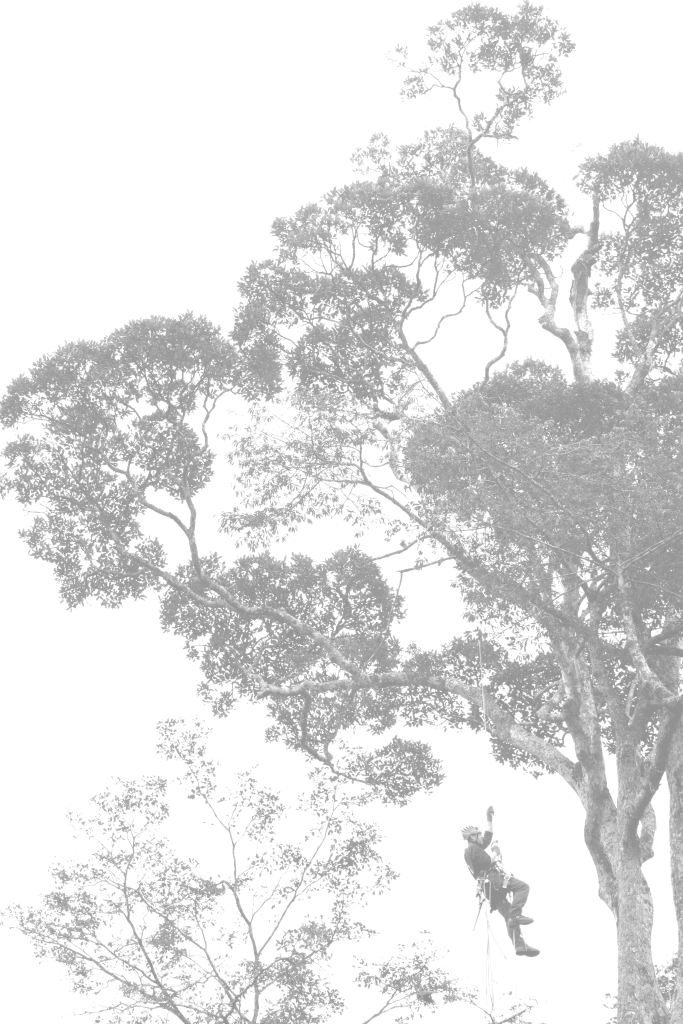
\includegraphics[width=\paperwidth/2]{filigrane}
  \end{textblock*}
  \begin{textblock*}{\paperwidth*2/3}(\spinemargin, \paperheight/2)
    {\fontfamily{qtm}\huge\theauthor}
  \end{textblock*}
    \begin{textblock*}{\paperwidth*2/3}[0, 1](\spinemargin, \uppermargin+\textheight)
    \normalfont\thedate
  \end{textblock*}
  ~\\ % Print a character or the page will not exist
  \newpage
  \textblockorigin{\trimedge}{\trimtop} % verso
  \begin{textblock*}{\textwidth}(\paperwidth-\spinemargin-\textwidth, \uppermargin)
    #1
  \end{textblock*}
  \begin{textblock*}{\textwidth}[0,1](\paperwidth-\spinemargin-\textwidth, \uppermargin+\textheight+\footskip)
    \centering
    
\includegraphics[width=\paperwidth/4]{logo}\\ \bigskip
    #2
  \end{textblock*}
  ~\\ % Print a character or the page will not exist
  \newpage
}

% Clear page and open an even one (\clearpage opens an odd one)
\newcommand{\evenpage}{
  \clearpage
  \strictpagecheck % slower but efficient detection of odd/even pages
  \checkoddpage
  \ifoddpage
    \thispagestyle{empty}
    ~\\ % Print a character or the page will not exist
    \newpage
  \else
    % do nothing
  \fi
}


%% PDF title page to insert
%%%%%%%%%%%%%%%%%%%%%%%%%%%%%%%%%%%%%%%%%%%%%%%%%%%%%%%%%%



%% Bibliography
%%%%%%%%%%%%%%%%%%%%%%%%%%%%%%%%%%%%%%%%%%%%%%%%%%%%%%%%%%

% Repeated citation as author-year-title instead of author-title (modification of footcite:note in verbose-inote.cbx)

%% Table of Contents
%%%%%%%%%%%%%%%%%%%%%%%%%%%%%%%%%%%%%%%%%%%%%%%%%%%%%%%%%%

% fix the typesetting of the part number
\renewcommand\partnumberlinebox[2]{#2\ ---\ }


% Fonts
%%%%%%%%%%%%%%%%%%%%%%%%%%%%%%%%%%%%%%%%%%%%%%%%%%%%%%%%%%


% Hyperref comes last
%%%%%%%%%%%%%%%%%%%%%%%%%%%%%%%%%%%%%%%%%%%%%%%%%%%%%%%%%%

\usepackage{hyperref}
\hypersetup{
  pdftitle={Travailler avec R},
  pdfauthor={Eric Marcon},
  colorlinks=true,
  linkcolor=Maroon,
  citecolor=Blue,
  urlcolor=Blue,
  breaklinks=true}

% Don't use monospace font for urls
\urlstyle{same}


% Title, author, date from YAML to LaTeX
%%%%%%%%%%%%%%%%%%%%%%%%%%%%%%%%%%%%%%%%%%%%%%%%%%%%%%%%%%

\title{Travailler avec R}

\author{Eric Marcon}

\date{01/02/2025}


% Include headers (preamble.tex) here
%%%%%%%%%%%%%%%%%%%%%%%%%%%%%%%%%%%%%%%%%%%%%%%%%%%%%%%%%%

\usepackage{booktabs}
\usepackage{longtable}
\usepackage{array}
\usepackage{multirow}
\usepackage{wrapfig}
\usepackage{float}
\usepackage{colortbl}
\usepackage{pdflscape}
\usepackage{tabu}
\usepackage{threeparttable}
\usepackage{threeparttablex}
\usepackage[normalem]{ulem}
\usepackage{makecell}
\usepackage{xcolor}
\usepackage{fontspec}
\usepackage{multicol}
\usepackage{hhline}
\newlength\Oldarrayrulewidth
\newlength\Oldtabcolsep
\usepackage{hyperref}


% End of preamble
%%%%%%%%%%%%%%%%%%%%%%%%%%%%%%%%%%%%%%%%%%%%%%%%%%%%%%%%%%


\begin{document}
\frontmatter

% Title page
%%%%%%%%%%%%%%%%%%%%%%%%%%%%%%%%%%%%%%%%%%%%%%%%%%%%%%%%%%


\MainTitlePage{Ce document est réalisé de façon dynamique et reproductible grâce à:

\begin{itemize}
  \item \LaTeX, dans sa distribution Miktex (\url{http://miktex.org/}) et la classe memoir (\url{http://www.ctan.org/pkg/memoir}).
  \item R (\url{http://www.r-project.org/}) et RStudio (\url{http://www.rstudio.com/})
  \item bookdown (\url{http://bookdown.org/}) et memoiR (\url{https://ericmarcon.github.io/memoiR/})
\end{itemize}

Son code source est sur GitHub: \url{https://github.com/EricMarcon/travailleR/}.

Le texte mis à jour en continu peut être lu sur \url{https://ericmarcon.github.io/travailleR/}.

Les versions d'étape sont déposées sur HAL: \url{https://hal.archives-ouvertes.fr/hal-03022820}.}{Photographie en couverture: Hadrien Lalagüe}


% Before Body
%%%%%%%%%%%%%%%%%%%%%%%%%%%%%%%%%%%%%%%%%%%%%%%%%%%%%%%%%%





% Contents
%%%%%%%%%%%%%%%%%%%%%%%%%%%%%%%%%%%%%%%%%%%%%%%%%%%%%%%%%%

\LargeMargins
{
\hypersetup{linkcolor=}
\setcounter{tocdepth}{2}
\tableofcontents
}


% Body
%%%%%%%%%%%%%%%%%%%%%%%%%%%%%%%%%%%%%%%%%%%%%%%%%%%%%%%%%%

\LargeMargins
\chapter*{Présentation}\label{pruxe9sentation}
\addcontentsline{toc}{chapter}{Présentation}

\section*{Objectifs}\label{objectifs}
\addcontentsline{toc}{section}{Objectifs}

Ce document est le support du cours \emph{Travailler avec R}.

Il propose une organisation du travail autour de R et RStudio pour, au-delà des statistiques, rédiger des documents efficacement avec R Markdown, aux formats variés (mémos, articles scientifiques, mémoires d'étudiants, livres, diaporamas), créer son site web et des applications R en ligne (Shiny), produire des packages et utiliser R pour l'enseignement.
Il complète \emph{Reproducible Research with R and R Studio} \autocite{Gandrud2013} par une approche plus concrète, avec des solutions prêtes à l'emploi.

L'optimisation de l'utilisation des nombreux outils disponibles est traitée en détail: \textbf{rmarkdown}, \textbf{bookdown} et \textbf{blogdown} pour la rédaction, \textbf{roxygen2}, \textbf{testthat} et \textbf{pkgdown} pour les packages, le contrôle de source avec git et GitHub, l'intégration continue avec les Actions GitHub et Codecov.
Des exemples sont présentés à chaque étape, et le code nécessaire est fourni.

Le chapitre \ref{chap-logiciels} est consacré à l'installation des outils nécessaires: R, git et LaTeX.
Le chapitre \ref{chap-utiliseR} détaille quelques aspects avancés de l'utilisation de R: les différents langages, les environnements, la performance du code.
L'utilisation de base de R n'est pas reprise ici: de bons cours sont suggérés.
Le chapitre \ref{chap-git} présente le contrôle de source avec git et GitHub.

Le chapitre \ref{chap-rediger} montre comment rédiger des documents simples (articles) ou complexes (ouvrages) avec R Markdown, intégrant les données, le code pour les traiter et le texte pour les présenter.
Le chapitre \ref{chap-package} présente une méthode pas à pas pour créer efficacement un package.
Le chapitre \ref{chap-ci} introduit l'utilisation de l'intégration continue pour produire automatiquement des documents, vérifier le code des packages et produire leurs vignettes.
Le chapitre \ref{chap-shiny} présente Shiny, l'outil de mise en ligne d'applications R.
Enfin, le chapitre \ref{chap-enseigner} introduit les outils destinés à l'enseignement avec R.

\section*{Conventions}\label{conventions}
\addcontentsline{toc}{section}{Conventions}

Les noms des packages sont en gras dans le texte, par exemple: \textbf{ggplot2}.

L'identifiant utilisé sur GitHub est noté \emph{GitHubID}.
Le nom des projets, identique à celui de leur dépôt sur GitHub est noté \emph{RepoID}.

Le signe \texttt{\textbar{}\textgreater{}} dans le code des exemples indique que la suite du code devrait se trouver sur la même ligne, mais est coupée pour le formatage de ce document.
Son usage est limité aux fichiers de configuration YAML, surtout utilisés dans le chapitre \ref{chap-ci}.
Dans tous les autres cas, le code peut être utilisé directement.

\mainmatter

\chapter{Logiciels}\label{chap-logiciels}

\toc{1}

L'outil central est évidemment R, mais son fonctionnement est aujourd'hui difficilement envisageable sans son environnement de développement RStudio.
Pour le contrôle de source, git et GitHub sont de fait les standards.
L'ensemble doit être complété par une distribution LaTeX pour la production de documents au format PDF.
Un outil de gestion bibliographique est indispensable: Zotero et son extension Better BibTeX sont parfaitement adaptés au cadre de travail présenté ici.
Enfin, d'autres logiciels d'usage plus ponctuel peuvent être nécessaires, comme Go.

Leur installation et leur organisation cohérente sont présentées dans ce chapitre.

\section{R}\label{r}

\subsection{Installation}\label{installation}

R est inclus dans les distributions de Linux: le paquet est nommé \texttt{r-base}.
Il ne contient pas des outils de développement souvent nécessaires, donc il est préférable d'installer aussi le paquet \texttt{r-base-dev}.
La version de R est souvent un peu ancienne.
Pour disposer de la dernière version, il faut utiliser un miroir de CRAN comme source des paquets: voir la documentation complète pour Ubuntu\footnote{\url{https://doc.ubuntu-fr.org/r}}.

Sous Windows ou Mac, installer R après l'avoir téléchargé depuis CRAN\footnote{\url{https://cran.r-project.org/}}.

\subsection{Rtools}\label{rtools}

Sur Mac, l'installation de R est suffisante à partir de la version 4.0.0.

Sous Windows, l'installation doit être complétée par les \enquote{Rtools}, qui contiennent les outils de développement dont ceux nécessaires à la compilation des packages contenant du code C++.

Le chemin des Rtools (avant la version 4.2) doit être déclaré à R, en exécutant dans la console de RStudio la commande suivante (adaptée à la version 4.0 des Rtools):

\scriptsize

\begin{Shaded}
\begin{Highlighting}[]
\CommentTok{\# Rtools : déclaration du chemin, }
\CommentTok{\# nécessite de redémarrer RStudio}
\FunctionTok{writeLines}\NormalTok{(}
  \StringTok{\textquotesingle{}PATH="$\{RTOOLS40\_HOME\}}\SpecialCharTok{\textbackslash{}\textbackslash{}}\StringTok{usr}\SpecialCharTok{\textbackslash{}\textbackslash{}}\StringTok{bin;$\{PATH\}"\textquotesingle{}}\NormalTok{,}
  \AttributeTok{con =} \StringTok{"\textasciitilde{}/.Renviron"}
\NormalTok{)}
\end{Highlighting}
\end{Shaded}

\normalsize

Depuis la version 4.2, cette action est inutile.

Les Rtools doivent être complétés par quelques utilitaires manquants, à installer quand le besoin apparaît (en général, un avertissement de R indiquant que le logiciel n'est pas installé).

La vérification des packages renvoie un avertissement si \emph{qpdf}\footnote{\url{https://sourceforge.net/projects/qpdf/}} n'est pas installé.
Télécharger le fichier zip et coller tout le contenu du dossier \texttt{bin} dans le dossier \texttt{usr/bin} de \texttt{Rtools} (\texttt{C:\textbackslash{}Rtools42\textbackslash{}usr\textbackslash{}bin} pour la version 4.2).

Un autre avertissement est renvoyé en absence de \emph{Ghostscript}\footnote{\url{https://www.ghostscript.com/}} à télécharger et installer.
Copier ensuite le contenu du dossier \texttt{bin} dans le dossier \texttt{usr/bin} de \texttt{Rtools}.

\subsection{Mise à jour}\label{mise-uxe0-jour}

Il est conseillé d'utiliser la dernière version mineure de R: par exemple, 4.0.x jusqu'à la sortie de la version 4.1.
Il est obligatoire d'utiliser la toute dernière version pour préparer un package soumis à CRAN.

Des changements importants ont lieu entre les versions majeures (la version 4 ne permet pas d'utiliser un package compilé pour la version 3) mais aussi parfois entre versions mineures (un fichier de données binaires \texttt{.rda} enregistré sous la version 3.3 ne peut pas être lu par la version 3.6).
Il est donc utile de mettre R à jour régulièrement.

L'installation d'une nouvelle version ne désinstalle par automatiquement les versions anciennes, ce qui permet d'en utiliser plusieurs en cas de besoin (par exemple, si un package ancien et indispensable n'est plus disponible).
En usage courant, il est préférable de désinstaller manuellement les anciennes versions après l'installation d'une nouvelle.

\subsection{Librairies}\label{sec:librairies}

Les packages de R se trouvent dans deux dossiers:

\begin{itemize}
\tightlist
\item
  la bibliothèque système (\emph{System Library}) contient les packages fournis avec R: \textbf{base}, \textbf{utils}, \textbf{graphics} par exemple.
  Elle se trouve dans un sous-répertoire du programme d'installation (\texttt{C:\textbackslash{}Program\ Files\textbackslash{}R\textbackslash{}R-4.1.0\textbackslash{}library} pour R version 4.1.0 sous Windows 10).
\item
  La bibliothèque utilisateur (\emph{User Library}) contient ceux installés par l'utilisateur.
  Jusqu'à la version 4.1, elle se trouve dans le dossier personnel de l'utilisateur, dans un sous-dossier \texttt{R\textbackslash{}win-library\textbackslash{}4.1\textbackslash{}}).
  Depuis la version 4.2, ce dossier se trouve dans les paramètres locaux de l'utilisateur dont l'emplacement du dossier se trouve dans la variable d'environnement \texttt{\%LOCALAPPDATA\%}.
\end{itemize}

Jusqu'à la version 4.1, si le dossier personnel de l'utilisateur est sauvegardé (par exemple, s'il est répliqué dans le cloud par OneDrive sous Windows), il n'est pas optimal d'y placer les packages: le trafic généré par leur sauvegarde serait lourd et inutile.
Pour que les packages soient installés automatiquement dans la bibliothèque système, il suffit que l'utilisateur y ait le droit d'écrire.
Sous Windows, donner le droit \enquote{Modifier} au groupe des utilisateurs de l'ordinateur sur le dossier de la bibliothèque, en plus du droit de lecture par défaut.
A partir de la version 4.2, il n'y a plus de raison de modifier le fonctionnement par défaut: les paramètres locaux ne sont pas sauvegardés.

Si la bibliothèque utilisateur est retenue, il faut penser à vider le dossier correspondant à l'ancienne version de R en cas changement de version mineure.

L'emplacement des librairies est donné par la fonction \texttt{.libPaths()}:

\scriptsize

\begin{Shaded}
\begin{Highlighting}[]
\FunctionTok{.libPaths}\NormalTok{()}
\end{Highlighting}
\end{Shaded}

\begin{verbatim}
## [1] "/Users/runner/work/_temp/Library"                                    
## [2] "/Library/Frameworks/R.framework/Versions/4.4-arm64/Resources/library"
\end{verbatim}

\normalsize

\section{RStudio}\label{rstudio}

RStudio est une interface graphique pour R et bien plus: il est conçu pour simplifier la gestion des projets, faciliter la rédaction et la production de documents et intégrer le contrôle de source par exemple.

\subsection{Installation}\label{installation-1}

Installer la dernière version de \emph{RStudio Desktop} à partir du site de RStudio\footnote{\url{https://rstudio.com/products/rstudio/download/}}.

Une commande est disponible dans le menu \enquote{Help} de RStudio pour vérifier l'existence d'une version plus récente, à installer.

\subsection{Encodage des fichiers}\label{encodage-des-fichiers}

Les fichiers manipulés dans R sont très majoritairement des fichiers texte.
Les caractères spéciaux, notamment les accents, peuvent être codés de diverses façons mais la déclaration du codage n'est pas intégrée aux fichiers.
Le codage par défaut dépend du système d'exploitation, ce qui pose régulièrement des problèmes de lisibilité des fichiers partagés.
Le codage UTF8 est devenu le standard parce qu'il est universellement reconnu et supporte tous les alphabets sans ambiguïtés.

Dès la première utilisation de RStudio, créer un nouveau fichier R (menu \enquote{File \textgreater{} New File \textgreater{} R Script}), l'enregistrer au format UTF8 (\enquote{File \textgreater{} Save with Encoding\ldots{}}), choisir UTF8 dans la liste des formats et cocher la case \enquote{Set as default encoding for source files}.
Supprimer le fichier après l'avoir enregistré.

Les nouveaux fichiers seront codés au format UTF8.
Les fichiers codés sous un autre format ne s'afficheront pas correctement: ils pourront être réouverts avec leur codage d'origine (\enquote{File \textgreater{} Reopen with Encoding\ldots{}}), en essayant éventuellement plusieurs codages jusqu'à obtenir un affichage correct, et sauvegardés au format UTF8 ensuite.

\subsection{Dossier de travail}\label{dossier-de-travail}

Le dossier de travail par défaut est le dossier personnel de l'utilisateur, appelé \texttt{\textasciitilde{}} par RStudio:

\scriptsize

\begin{Shaded}
\begin{Highlighting}[]
\FunctionTok{Sys.getenv}\NormalTok{(}\StringTok{"R\_USER"}\NormalTok{)}
\end{Highlighting}
\end{Shaded}

\begin{verbatim}
## [1] ""
\end{verbatim}

\normalsize

\begin{itemize}
\tightlist
\item
  \texttt{Mes\ Documents} sous Windows;
\item
  \texttt{Home} sous Mac ou Linux.
\end{itemize}

Il faut systématiquement travailler dans des sous-dossiers de \texttt{\textasciitilde{}}, par exemple: \texttt{\textasciitilde{}/Formation}.

Pour le bon fonctionnement des \emph{RTools}, le nom complet du répertoire de travail ne doit pas contenir d'espace (utiliser les tirets bas \texttt{\_}) ni de caractère spécial.
Le dossier de travail en cours est obtenu par la commande \texttt{getwd()}.

\scriptsize

\begin{Shaded}
\begin{Highlighting}[]
\FunctionTok{getwd}\NormalTok{()}
\end{Highlighting}
\end{Shaded}

\normalsize

L'utilisation du contrôle de source (voir chapitre \ref{chap-git}) crée de nombreux fichiers de travail.
Les projets sous contrôle de source ne devraient pas se trouver dans un dossier déjà sauvegardé par un autre moyen, comme un lecteur OneDrive sous Windows, sous peine d'une utilisation excessive des ressources: chaque validation de modifications engendre la sauvegarde des fichiers modifiés, mais aussi des fichiers de contrôle qui peuvent être de grande taille.

\subsection{Solution retenue}\label{sec:solution-dossiers}

L'organisation de l'environnement travail est une affaire personnelle, qui dépend des préférences de chacun.
L'organisation proposée ici n'est qu'une possibilité, à adapter à ses propres choix, mais en respectant les contraintes mentionnées.

Sous Windows, une organisation optimale est la suivante:

\begin{itemize}
\tightlist
\item
  Dans son dossier personnel (\texttt{Mes\ Documents}, \texttt{\textasciitilde{}} pour R), un dossier \texttt{R} est utilisé pour les projets simples, sans contrôle de source.
  La sauvegarde de ce dossier est gérée par ailleurs.
\item
  Un dossier hors du dossier personnel est utilisé pour les projets sous contrôle de source.
  L'utilisateur doit y avoir le droit d'écrire.
  Dans l'organisation de Windows, le dossier correspondant à ces critères est \texttt{\%LOCALAPPDATA\%}, typiquement \texttt{C:\textbackslash{}Users\textbackslash{}NomUtilisateur\textbackslash{}AppData}\break\texttt{\textbackslash{}Local}.
  Le dossier sera donc \texttt{\%LOCALAPPDATA\%\textbackslash{}ProjetsR} à créer: exécuter \texttt{md\ \%LOCALAPPDATA\%\textbackslash{}ProjetsR} dans une invite de commande.
  Epingler ce dossier à l'accès rapide de l'explorateur de fichiers (figure \ref{fig:R-ProjetsR}): coller \texttt{\%LOCALAPPDATA\%\textbackslash{}ProjetsR} dans la barre d'adresse de l'explorateur de fichiers, valider, puis faire un clic droit sur \enquote{Accès Rapide} et épingler le dossier.
\end{itemize}



\scriptsize

\begin{figure}

{\centering 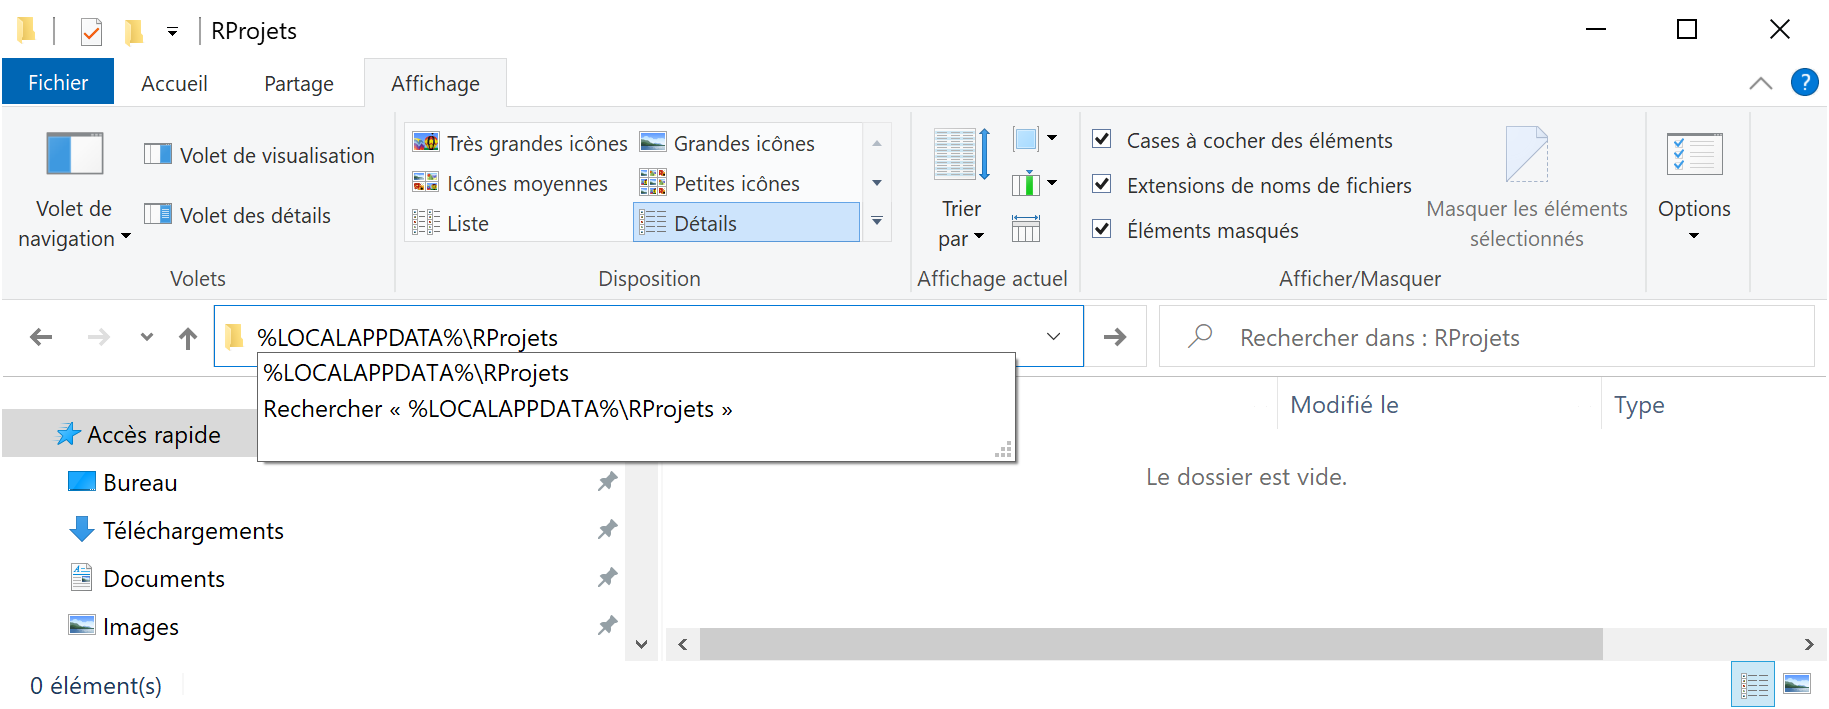
\includegraphics[width=1\linewidth]{images/R-ProjetsR} 

}

\caption{Dossier pour les projets sous contrôle de source, sous Windows.}\label{fig:R-ProjetsR}
\end{figure}

\normalsize

\subsection{Police de caractères}\label{police-de-caractuxe8res}

La police Fira Code\footnote{\url{https://github.com/tonsky/FiraCode}} fournit des ligatures: les caractères \enquote{\textless-} utilisés pour l'assignation dans R sont par exemple affichés comme une flèche.
Pour l'utiliser dans l'éditeur de RStudio, il suffit de l'installer en suivant les instructions appropriées à son système d'exploitation et de la déclarer dans les options globales (menu \enquote{Tools \textgreater{} Global Options\ldots{}}): sélectionner \emph{Appearance} et l'option \emph{Editor Font}: Fira Code.

\section{Packages}\label{packages}

\subsection{Installation depuis CRAN}\label{installation-depuis-cran}

L'installation classique des packages fait appel à CRAN.
Un bouton \enquote{Install} se trouve dans la fenêtre \emph{Packages} de RStudio.

Les packages sont déposés sur CRAN par leurs auteur sous forme de code source, compressé dans une fichier \texttt{.tar.gz}.
Ils sont disponibles pour le téléchargement dès leur validation.
Ils doivent ensuite être mis au format binaire pour Windows (dans un fichier \texttt{.zip}), ce qui prend un peu de temps.

A la demande de l'installation d'un package sous Windows, CRAN propose la version source plutôt que la version binaire si elle est plus récente \ref{fig:R-BinaryPkg}).



\scriptsize

\begin{figure}

{\centering 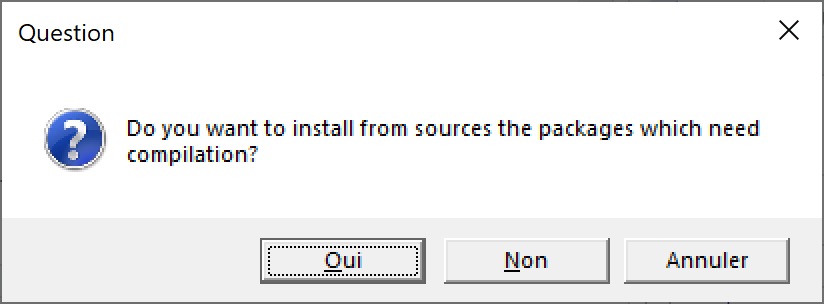
\includegraphics[width=0.8\linewidth]{images/R-BinaryPkg} 

}

\caption{Choix de la version des packages à installer.}\label{fig:R-BinaryPkg}
\end{figure}

\normalsize

La liste des packages concernés est affichée dans la console, par exemple:

\begin{verbatim}
  There are binary versions available but the source 
  versions are later:
              binary   source needs_compilation
boot          1.3-24   1.3-25             FALSE
class         7.3-16   7.3-17              TRUE
\end{verbatim}

Certains packages nécessitent une compilation (colonne \texttt{needs\_compilation}), en général parce qu'ils contiennent du code C++.
Ils ne pourront être installés que par les \emph{Rtools}.

L'installation des packages en version source est beaucoup plus longue qu'en version binaire.
Sauf si une version précise d'un package est nécessaire, il est donc préférable de refuser l'installation des versions source.

Les packages peuvent être mis à jour un peu plus tard, après leur compilation par CRAN.

Le bouton \enquote{Update} dans la fenêtre \emph{Packages} de RStudio permet de mettre à jour tous les packages installés.

\subsection{Installation depuis GitHub}\label{installation-depuis-github}

Certains packages ne sont pas disponibles sur CRAN mais seulement sur GitHub parce qu'ils sont encore en développement ou parce qu'ils ne sont pas destinés à un large usage par la communauté des utilisateurs de R.
Il peut aussi être utile d'installer une version de développement d'un package publié sur CRAN pour un usage ponctuel comme le test de nouvelles fonctionnalités.

L'installation est gérée par le package \textbf{remotes}.
L'argument \texttt{build\_vignettes} est nécessaire pour créer les vignettes du package.

\scriptsize

\begin{Shaded}
\begin{Highlighting}[]
\NormalTok{remotes}\SpecialCharTok{::}\FunctionTok{install\_github}\NormalTok{(}\StringTok{"EricMarcon/memoiR"}\NormalTok{, }\AttributeTok{build\_vignettes =} \ConstantTok{TRUE}\NormalTok{)}
\end{Highlighting}
\end{Shaded}

\normalsize

Le nom du package est entré sous la forme \enquote{GitHubID/NomduPackage}.
L'installation est faite à partir du code source et nécessite donc les \emph{Rtools} si une compilation est nécessaire.
\texttt{install\_github()} vérifie que la version sur GitHub est plus récente que l'éventuelle version installée sur le poste de travail et ne fait rien si elles sont identiques.

\subsection{Installation depuis Bioconductor}\label{installation-depuis-bioconductor}

Bioconductor est une plateforme complémentaire de CRAN qui héberge des packages spécialisés dans la génomique.
L'installation des packages de Bioconductor nécessite le package \textbf{BiocManager} pour sa fonction \texttt{install()}.
Le premier argument de la fonction est un vecteur de caractères contenant les noms des packages à installer, par exemple:

\scriptsize

\begin{Shaded}
\begin{Highlighting}[]
\NormalTok{BiocManager}\SpecialCharTok{::}\FunctionTok{install}\NormalTok{(}\FunctionTok{c}\NormalTok{(}\StringTok{"GenomicFeatures"}\NormalTok{, }\StringTok{"AnnotationDbi"}\NormalTok{))}
\end{Highlighting}
\end{Shaded}

\normalsize

La fonction \texttt{install()} appelée sans arguments met à jour les packages.

\subsection{Solution retenue}\label{solution-retenue}

A chaque mise à jour mineure de R, tous les packages doivent être réinstallés.
La façon la plus efficace de le faire est de créer un script \texttt{Packages.R} à placer dans \texttt{\textasciitilde{}\textbackslash{}R}.
Il contient une fonction qui vérifie si chaque package est déjà installé pour ne pas le refaire inutilement.

\scriptsize

\begin{Shaded}
\begin{Highlighting}[]
\CommentTok{\# Installation des packages de R \#\#\#\#}

\CommentTok{\# Installer les packages si nécessaire \#\#\#\#}
\NormalTok{install\_packages }\OtherTok{\textless{}{-}} \ControlFlowTok{function}\NormalTok{(packages) \{}
\NormalTok{  install\_package }\OtherTok{\textless{}{-}} \ControlFlowTok{function}\NormalTok{(package) \{}
    \ControlFlowTok{if}\NormalTok{ (}\SpecialCharTok{!}\NormalTok{package }\SpecialCharTok{\%in\%} \FunctionTok{installed.packages}\NormalTok{()[, }\DecValTok{1}\NormalTok{]) \{}
      \FunctionTok{install.packages}\NormalTok{(package, }\AttributeTok{repos =} \StringTok{"https://cran.rstudio.com/"}\NormalTok{)}
\NormalTok{    \}}
\NormalTok{  \}}
  \FunctionTok{invisible}\NormalTok{(}\FunctionTok{sapply}\NormalTok{(packages, install\_package))}
\NormalTok{\}}

\CommentTok{\# Outils de développement \#\#\#\#}
\FunctionTok{install\_packages}\NormalTok{(}
  \FunctionTok{c}\NormalTok{(}
    \CommentTok{\# Development tools. Import remotes, etc.}
    \StringTok{"devtools"}\NormalTok{,}
    \CommentTok{\# Run Check by RStudio}
    \StringTok{"rcmdcheck"}\NormalTok{,}
    \CommentTok{\# Formatting R code (used by knitr)}
    \StringTok{"formatR"}\NormalTok{,}
    \CommentTok{\# Documentation of packages in /docs on GitHub}
    \StringTok{"pkgdown"}\NormalTok{,}
    \CommentTok{\# Bibliography with roxygen}
    \StringTok{"Rdpack"}\NormalTok{,}
    \CommentTok{\# Performance measurement}
    \StringTok{"rbenchmark"}\NormalTok{,}
    \CommentTok{\# Automatic package documentation}
    \StringTok{"roxygen2"}\NormalTok{,}
    \CommentTok{\# Package testing}
    \StringTok{"testthat"}
\NormalTok{  )}
\NormalTok{)}

\CommentTok{\# Markdown \#\#\#\#}
\FunctionTok{install\_packages}\NormalTok{(}
  \FunctionTok{c}\NormalTok{(}
    \CommentTok{\# Knit}
    \StringTok{"knitr"}\NormalTok{,}
    \CommentTok{\# Complex markdown documents}
    \StringTok{"bookdown"}\NormalTok{,}
    \CommentTok{\# Websites}
    \StringTok{"blogdown"}\NormalTok{,}
    \CommentTok{\# Document templates}
    \StringTok{"memoiR"}
\NormalTok{  )}
\NormalTok{)}

\CommentTok{\# Tidyverse \#\#\#\#}
\FunctionTok{install\_packages}\NormalTok{(}\StringTok{"tidyverse"}\NormalTok{)}
\end{Highlighting}
\end{Shaded}

\normalsize

La dernière partie du script est à compléter avec les packages utilisés régulièrement.

Ce script est à exécuter à chaque mise à jour de R, après avoir éventuellement activé le droit d'écriture dans la librairie système (voir section \ref{sec:librairies}).

\section{git et GitHub}\label{git-et-github}

\subsection{git}\label{git}

git est le logiciel de contrôle de source utilisé ici.
Son utilisation est détaillée dans le chapitre \ref{chap-git}.

Pour Windows et Mac, l'installation a lieu à partir du site web de git\footnote{\url{https://git-scm.com/}}.

git est intégré dans les distributions Linux.
Pour Ubuntu, le package apt est \texttt{git-all}.

git est installé sans interface graphique, fournie par RStudio.

Dans RStudio, modifier les options globales (menu \enquote{Tools \textgreater{} Global Options\ldots{}}).
Sélectionner \emph{Terminal} et l'option \emph{New Terminals open with}: GitBash.

Vérifier la bonne installation de git en tapant la commande \texttt{git\ -h} dans le terminal de RStudio: l'aide doit s'afficher.

Après l'installation de git, il est possible que le terminal de RStudio ne fonctionne plus correctement et renvoie un message d'erreur contenant les éléments suivants:

\begin{verbatim}
*** fatal error - cygheap base mismatch detected
This problem is probably due to using incompatible 
versions of the cygwin DLL.
\end{verbatim}

Le message d'erreur est imprécis: la librairie qui ne doit exister qu'en un seul exemplaire n'est pas \texttt{cygwin1.dll} mais \texttt{msys-2.0.dll}.
Rechercher ce fichier dans les dossier d'installation de git et de Rtools.
Ils se trouvent normalement dans \texttt{usr/bin}.
Remplacer celui de git par celui de Rtools: la version des deux fichiers doit être identique.

Entrer ses informations d'identification en exécutant les commandes suivantes dans le terminal:

\begin{verbatim}
git config user.name
git config user.email
\end{verbatim}

Le nom d'utilisateur est libre, de préférence \enquote{Prénom Nom}.

\subsection{GitHub}\label{github}

\emph{GitHub} est la plateforme accessible par un \href{https://github.com/}{site web} qui permet de partager le contenu des dépôts \emph{git}.
Pour l'utiliser, il suffit d'ouvrir un compte avec la même adresse de messagerie que celle enregistrée dans git.

Le nom du compte GitHub est noté ici \emph{GitHubID}.
Chaque compte GitHub permet d'héberger des dépôts (un dépôt contient les fichiers d'un projet) à l'adresse \url{https://github.com/GitHubID/NomDuDepot}\footnote{Exemple: \url{https://github.com/EricMarcon/travailleR}}.
Chaque dépôt peut disposer d'un site web à l'adresse \url{https://GitHubID.github.io/NomDuDepot/}\footnote{Exemple: \url{https://EricMarcon.github.io/travailleR/}}.
Enfin, un site web global est prévu pour chaque utilisateur à l'adresse \url{https://GitHubID.github.io/}\footnote{Exemple: \url{https://EricMarcon.github.io/}}.

\subsection{Authentification SSH}\label{sec:SSH}

La communication entre git (installé sur l'ordinateur local) et GitHub (plateforme en ligne) nécessite de s'authentifier.

Deux méthodes sont disponibles: HTTPS (aussi appelée SSL) et SSH.
SSH est la plus robuste mais nécessite la création d'une clé privée.

Dans le terminal de RStudio, exécuter:

\begin{verbatim}
ssh-keygen -t ed25519 -C "user.email"
\end{verbatim}

L'adresse de messagerie (qui remplace \enquote{user.email}) doit être celle enregistrée dans la configuration de git et le compte GitHub.
La clé est enregistrée dans le dossier \texttt{.ssh} du répertoire personnel de l'utilisateur.
Il est possible d'ajouter un mot de passe (\emph{passphrase}) à la clé, qui devra être tapé à la première utilisation de chaque session de travail.
Si l'ordinateur est correctement sécurisé (pas d'accès physique par des tiers), la laisser vide permet de gagner en fluidité.

Attention: la clé privée est strictement confidentielle et ne doit être copiée nulle part où elle pourrait être lue par un tiers (attention aux sauvegardes automatiques notamment).
Elle n'a pas besoin d'être bien sauvegardée: en cas de perte, elle sera remplacée facilement.

Les clés sont normalement stockées dans le dossier \texttt{\textasciitilde{}/.ssh}, quel que soit le système d'exploitation, mais l'emplacement du dossier personnel \texttt{\textasciitilde{}} est ambiguë sous Windows: pour R, c'est le dossier \texttt{Documents}, mais pour d'autres logiciels, c'est le dossier racine de l'utilisateur, parent de \texttt{Documents}.

Dans le terminal de RStudio, vérifier le bon fonctionnement de la clé:

\begin{verbatim}
ssh -T git@github.com
\end{verbatim}

Si un message d'erreur indique qu'aucune clé n'est trouvée, deux solutions sont possibles:

\begin{itemize}
\tightlist
\item
  Dupliquer le dossier \texttt{.ssh} (avec l'explorateur de fichiers) dans \texttt{Documents};
\item
  Dupliquer le dossier \texttt{.ssh} dans le dossier du programme RStudio (généralement \texttt{C:\textbackslash{}Program\ Files\textbackslash{}RStudio\textbackslash{}}), dans \texttt{resources\textbackslash{}terminal\textbackslash{}bash\textbackslash{}}.
\end{itemize}

En cas de succès, un message indique que l'authenticité du serveur GitHub ne peut pas être vérifiée: un contrôle manuel est nécessaire pour la première connexion.
Vérifier auprès de GitHub que l'empreinte du serveur est correcte\footnote{\url{https://docs.github.com/en/github/authenticating-to-github/githubs-ssh-key-fingerprints}} et taper \texttt{yes}.
Le serveur est ajouté automatiquement à la liste des serveurs connus, dans le fichier \texttt{known\_hosts}.

Dans le dossier \texttt{.ssh}, deux fichiers sont créés: l'un contient la clé privée, l'autre, avec l'extension \texttt{.pub}, la clé publique correspondante.
Ouvrir le second avec un éditeur de texte et copier la clé publique dans le presse-papier.
Sur GitHub, afficher les réglages de son compte (menu \enquote{Settings}), sélectionner \enquote{SSH and GPG Keys}, cliquer sur \enquote{New SSH Key} et coller la clé dans le champ \enquote{Key}.
Donner un nom à la clé dans le champ \enquote{Title}.
Le nom peut être celui de l'ordinateur sur lequel la clé a été créée.
La clé ne doit pas être copiée sur plusieurs ordinateurs: en cas de besoin, créer une nouvelle clé sur chaque poste de travail utilisé.

Si la clé est compromise (perte ou prêt de l'ordinateur qui la contient), la supprimer sur GitHub et en créer une nouvelle.

\subsection{Obtention d'un jeton d'accès personnel}\label{sec:pat}

L'authentification HTTPS est l'alternative à l'authentification SSL: il faut choisir une méthode et s'y tenir par la suite.
Pour utiliser l'authentification HTTPS, la création d'un jeton d'accès personnel est nécessaire.

Les jetons sont créés sur GitHub, dans les paramètres de son compte d'utilisateur, dans \enquote{Developer Settings \textgreater{} Personal Access Tokens}\footnote{\url{https://help.github.com/en/github/authenticating-to-github/creating-a-personal-access-token-for-the-command-line}}.

Générer un nouveau jeton, le décrire en tant que \enquote{git-RStudio} et lui donner l'autorisation \enquote{repo}, c'est-à-dire modifier \emph{tous} les dépôts (il n'est pas possible de limiter l'accès à un dépôt particulier).
Le jeton est une chaîne de caractère qui ne pourra pas être relue plus tard: elle doit être sauvegardée comme un mot de passe.

\section{Compilateur LaTeX}\label{compilateur-latex}

Pour produire des documents au format PDF, une distribution LaTeX est nécessaire.
La solution légère consiste à installer le package \textbf{tinytex} qui installe à son tour une distribution LaTeX optimisée pour R Markdown.

Une distribution complète permet l'utilisation de LateX au-delà de RStudio mais est inutile si l'usage de LaTeX se limite au tricot de documents R Markdown.
MiKTeX est une très bonne solution pour Windows et Mac.

\subsection{tinytex}\label{tinytex}

Installer le package puis exécuter:

\scriptsize

\begin{Shaded}
\begin{Highlighting}[]
\NormalTok{tinytex}\SpecialCharTok{::}\FunctionTok{install\_tinytex}\NormalTok{()}
\end{Highlighting}
\end{Shaded}

\normalsize

L'ajout de packages LaTeX non inclus dans la distribution minimale de départ est automatique mais peut être lente.

La distribution peut être mise à jour par la commande:

\scriptsize

\begin{Shaded}
\begin{Highlighting}[]
\NormalTok{tinytex}\SpecialCharTok{::}\FunctionTok{tlmgr\_update}\NormalTok{()}
\end{Highlighting}
\end{Shaded}

\normalsize

\subsection{MiKTeX}\label{miktex}

\subsubsection{Installation}\label{installation-2}

Télécharger le fichier d'installation\footnote{\url{https://miktex.org/download}} et l'exécuter.
Plusieurs choix sont à faire pendant l'installation:

\begin{itemize}
\tightlist
\item
  Installer le programme pour tous les utilisateurs (avec des droits d'administrateur);
\item
  Le format par défaut du papier: choisir A4;
\item
  Le mode d'installation des packages manquants: choisir \enquote{Always Install} pour qu'ils soient téléchargés automatiquement en cas de besoin.
\end{itemize}

Pour Linux, suivre les instructions sur le site de MiKTeX.

\subsubsection{Mises à jour}\label{mises-uxe0-jour}

MiKTeX est installé avec les packages LaTeX les plus utilisés.
Si un document nécessite un package manquant, il est chargé automatiquement.
Les mises à jour de packages doivent être faites périodiquement avec la console MiKTeX, accessible dans le menu Démarrer.

Quand elle est lancée sans élévation des privilèges, la console propose de passer en mode administrateur.
Cliquer sur \enquote{Switch to Administrator mode}.

Dans les paramètres (\emph{Settings}), vérifier que les packages s'installent toujours automatiquement et que le format du papier est bien A4.

Dans le menu des mises à jour (\emph{Updates}), cliquer sur \enquote{Check for updates} puis \enquote{Update now}.

Si l'installation automatique est défaillante, il est possible d'installer manuellement un package dans le menu \enquote{Packages}.

\section{Zotero}\label{sec:Zotero}

Zotero\footnote{\url{https://www.zotero.org/}} est le logiciel de gestion bibliographique le plus utilisé.
Ses extensions permettent de compléter ses fonctionnalités selon les besoins de chacun.
Better BibTeX permet d'exporter et de maintenir à jour une sélection des références bibliographiques (une collection de Zotero) sous la forme d'un fichier BibTeX dans un projet R, où il pourra être utilisé dans la rédaction de documents ou la documentation de packages.

Télécharger le fichier d'installation et l'exécuter.
Créer un compte utilisateur sur le site web de Zotero.
Lier l'installation locale au compte: dans le menu \enquote{Edition \textgreater{} Paramètres}, sélectionner \enquote{Synchronisation} et s'authentifier dans la zone \enquote{Synchronisation des données}.
Cocher ensuite la case \enquote{Synchroniser automatiquement} mais pas \enquote{Synchroniser le texte intégral des pièces jointes indexées} parce que la taille totale des textes intégraux synchronisés de cette manière entre le compte Zotero en ligne et le poste de travail est limitée à 300 Mo.
Désactiver ensuite les deux options dans Synchronisation des fichiers.

Télécharger l'extension Better BibTeX\footnote{\url{https://retorque.re/zotero-better-bibtex/installation/}} et l'installer avec le menu \enquote{Outils \textgreater{} Extensions}: cliquer sur le bouton des paramètres en haut à droite de la fenêtre, puis \enquote{Install Add-on From File\ldots{}} et sélectionner le fichier qui vient d'être téléchargé.

Paramétrer Better BibTeX à partir du menu \enquote{Edition \textgreater{} Paramètres}, \enquote{Better BibTeX}.
Les options à modifier sont les suivantes:

\begin{itemize}
\tightlist
\item
  \enquote{Clés de citation \textgreater{} Format de clé}: \texttt{{[}auth:capitalize{]}{[}year{]}} pour que les citations disposent d'un identifiant unique de la forme \enquote{Nom2021};
\item
  \enquote{Clés de citation \textgreater{} Conserver les clés de citation uniques dans}: \enquote{Toutes les collections} pour que les identifiants des citations ne soient pas ambigus;
\item
  \enquote{Exportation \textgreater{} Gestion des Champs \textgreater{} Champs à exclure de l'exportation}: \enquote{abstract, file} pour ne pas générer des fichiers bibliographiques surchargés d'informations inutiles dans les projets R.
\end{itemize}

Il est conseillé d'utiliser l'extension ZotMoov\footnote{\url{http://https://github.com/wileyyugioh/zotmoov/}} pour mieux contrôler l'emplacement du texte intégral (les fichiers PDF liés au références bibliographiques).
L'installer puis la paramétrer dans \enquote{Edition \textgreater{} Paramètres}, \enquote{ZotMoov}.
Choisir le dossier de stockage des textes intégraux dans \enquote{Directory to Move Files To}.
Si le dossier personnel de l'utilisateur est sauvegardé (par exemple, s'il est répliqué dans le cloud par OneDrive sous Windows), y placer ce dossier de stockage permet à la fois de sauvegarder les textes intégraux mais aussi d'y accéder à partir de plusieurs postes de travail ou directement en ligne.
Cette solution est bien plus efficace que la synchronisation par défaut de Zotero, limitée en volume.

Sélectionner ensuite le dossier de téléchargement dans \enquote{Source Folder for Attaching New Files}.
Le menu contextuel \enquote{ZotMoov: Attach New File} permettra alors de lier automatiquement le dernier fichier téléchargé à la référence choisie.

Enfin, dans les options avancées de Zotero (\enquote{Edition \textgreater{} Paramètres}, \enquote{Avancé}), choisir le répertoire de base pour les pièces jointes liées: ce doit être le même que celui choisi pour le stockage des textes intégraux.

\section{Go}\label{go}

Go\footnote{\url{https://golang.org/}} n'est utilisé que par le générateur de sites web Hugo (voir section \ref{sec:blogdown}).

Télécharger le fichier d'installation et l'exécuter.
A la fin de l'installation, exécuter la commande \texttt{go\ version} dans un terminal pour vérifier son bon fonctionnement.

Les mises à jour se font en installant la nouvelle version par dessus la précédente.

\chapter{Utiliser R}\label{chap-utiliseR}

\toc{1}

La documentation consacrée à l'apprentissage de R est florissante.
Les ouvrages suivants sont une sélection arbitraire mais utile pour progresser:

\begin{itemize}
\tightlist
\item
  L'\href{https://juba.github.io/tidyverse/}{Introduction à R et au tidyverse} \autocite{Barnier2020} est un excellent cours de prise en main.
\item
  \href{http://adv-r.had.co.nz/}{Advanced R} \autocite{Wickham2014} est la référence pour maîtriser les subtilités du langage et bien comprendre le fonctionnement de R.
\item
  \href{https://r4ds.had.co.nz/}{R for Data Science} \autocite{Wickham2016} présente une méthode de travail complète, cohérente avec le tidyverse.
\item
  Enfin, \href{https://csgillespie.github.io/efficientR/}{Efficient R programming} \autocite{Gillespie2016} traite de l'optimisation du code.
\end{itemize}

Quelques aspects avancés du codage sont vus ici.
Des précisions sur les différents langages de R sont utiles pour la création de packages.
Les environnements sont présentés ensuite, pour la bonne compréhension de la recherche des objets appelés par le code.
Enfin, l'optimisation des performances du code est traitée en détail (boucles, code C++ et parallélisation) et illustrée par une étude de cas.

\section{Les langages de R}\label{les-langages-de-r}

R comprend plusieurs langages de programmation.
Le plus courant est S3, mais ce n'est pas le seul\footnote{\url{https://adv-r.had.co.nz/OO-essentials.html}}.

\subsection{Base}\label{base}

Le cœur de R est constitué des fonctions primitives et structures de données de base comme la fonction \texttt{sum} et les données de type \texttt{matrix}:

\scriptsize

\begin{Shaded}
\begin{Highlighting}[]
\NormalTok{pryr}\SpecialCharTok{::}\FunctionTok{otype}\NormalTok{(sum)}
\end{Highlighting}
\end{Shaded}

\begin{verbatim}
## [1] "base"
\end{verbatim}

\begin{Shaded}
\begin{Highlighting}[]
\FunctionTok{typeof}\NormalTok{(sum)}
\end{Highlighting}
\end{Shaded}

\begin{verbatim}
## [1] "builtin"
\end{verbatim}

\begin{Shaded}
\begin{Highlighting}[]
\NormalTok{pryr}\SpecialCharTok{::}\FunctionTok{otype}\NormalTok{(}\FunctionTok{matrix}\NormalTok{(}\DecValTok{1}\NormalTok{))}
\end{Highlighting}
\end{Shaded}

\begin{verbatim}
## [1] "base"
\end{verbatim}

\begin{Shaded}
\begin{Highlighting}[]
\FunctionTok{typeof}\NormalTok{(}\FunctionTok{matrix}\NormalTok{(}\DecValTok{1}\NormalTok{))}
\end{Highlighting}
\end{Shaded}

\begin{verbatim}
## [1] "double"
\end{verbatim}

\normalsize

Le package \textbf{pryr} permet d'afficher le langage dans lequel des objets sont définis.
La fonction \texttt{typeof()} affiche le type de stockage interne des objets:

\begin{itemize}
\tightlist
\item
  la fonction \texttt{sum()} appartient au langage de base de R et est une fonction primitive (\emph{builtin});
\item
  les éléments de la matrice numérique contenant un seul 1 sont des réels à double précision, et la matrice elle-même est définie dans le langage de base.
\end{itemize}

Les fonctions primitives sont codées en C et sont très rapides.
Elles sont toujours disponibles, quels que soient les packages chargés.
Leur usage est donc à privilégier.

\subsection{S3}\label{sec:S3}

S3 est le langage le plus utilisé, souvent le seul connu par les utilisateurs de R.

C'est un langage orienté objet dans lequel les classes, c'est-à-dire le type des objets, sont déclaratives.

\scriptsize

\begin{Shaded}
\begin{Highlighting}[]
\NormalTok{MonPrenom }\OtherTok{\textless{}{-}} \StringTok{"Eric"}
\FunctionTok{class}\NormalTok{(MonPrenom) }\OtherTok{\textless{}{-}} \StringTok{"Prenom"}
\end{Highlighting}
\end{Shaded}

\normalsize

La variable \texttt{MonPrenom} est ici de classe \enquote{Prenom} par une simple déclaration.

Contrairement au fonctionnement d'un langage orienté objet classique\footnote{\url{https://www.troispointzero.fr/le-blog/introduction-a-la-programmation-orientee-objet-poo/}}, les méthodes S3 sont liées aux fonctions, pas aux objets.

\scriptsize

\begin{Shaded}
\begin{Highlighting}[]
\CommentTok{\# Affichage par défaut}
\NormalTok{MonPrenom}
\end{Highlighting}
\end{Shaded}

\begin{verbatim}
## [1] "Eric"
## attr(,"class")
## [1] "Prenom"
\end{verbatim}

\begin{Shaded}
\begin{Highlighting}[]
\NormalTok{print.Prenom }\OtherTok{\textless{}{-}} \ControlFlowTok{function}\NormalTok{(x) }\FunctionTok{cat}\NormalTok{(}\StringTok{"Le prénom est"}\NormalTok{, x) }
\CommentTok{\# Affichage modifié}
\NormalTok{MonPrenom}
\end{Highlighting}
\end{Shaded}

\begin{verbatim}
## Le prénom est Eric
\end{verbatim}

\normalsize

Dans cet exemple, la méthode \texttt{print()} appliquée à la classe \enquote{Prenom} est modifiée.
Dans un langage orienté objet classique, la méthode serait définie dans la classe \texttt{Prenom}.
Dans R, les méthodes sont définies à partir de méthodes génériques.

\texttt{print} est une méthode générique (\enquote{un générique}) déclaré dans \textbf{base}.

\scriptsize

\begin{Shaded}
\begin{Highlighting}[]
\NormalTok{pryr}\SpecialCharTok{::}\FunctionTok{otype}\NormalTok{(print)}
\end{Highlighting}
\end{Shaded}

\begin{verbatim}
## [1] "base"
\end{verbatim}

\normalsize

Son code se résume à une déclaration \texttt{UseMethod("print")}:

\scriptsize

\begin{Shaded}
\begin{Highlighting}[]
\NormalTok{print}
\end{Highlighting}
\end{Shaded}

\begin{verbatim}
## function (x, ...) 
## UseMethod("print")
## <bytecode: 0x142288a38>
## <environment: namespace:base>
\end{verbatim}

\normalsize

Il existe beaucoup de méthodes S3 pour \texttt{print}:

\scriptsize

\begin{Shaded}
\begin{Highlighting}[]
\FunctionTok{head}\NormalTok{(}\FunctionTok{methods}\NormalTok{(}\StringTok{"print"}\NormalTok{))}
\end{Highlighting}
\end{Shaded}

\begin{verbatim}
## [1] "print.acf"               "print.activeConcordance"
## [3] "print.AES"               "print.all_vars"         
## [5] "print.anova"             "print.any_vars"
\end{verbatim}

\normalsize

Chacune s'applique à une classe. \texttt{print.default} est utilisée en dernier ressort et s'appuie sur le type de l'objet, pas sur sa classe S3.

\scriptsize

\begin{Shaded}
\begin{Highlighting}[]
\FunctionTok{typeof}\NormalTok{(MonPrenom)}
\end{Highlighting}
\end{Shaded}

\begin{verbatim}
## [1] "character"
\end{verbatim}

\begin{Shaded}
\begin{Highlighting}[]
\NormalTok{pryr}\SpecialCharTok{::}\FunctionTok{otype}\NormalTok{(MonPrenom)}
\end{Highlighting}
\end{Shaded}

\begin{verbatim}
## [1] "S3"
\end{verbatim}

\normalsize

Un objet peut appartenir à plusieurs classes, ce qui permet une forme d'héritage des méthodes.
Dans un langage orienté objet classique, l'héritage permet de définir des classes plus précises (\enquote{PrenomFrancais}) qui héritent de classes plus générales (\enquote{Prenom}) et bénéficient de cette façon de leurs méthodes sans avoir à les redéfinir.
Dans R, l'héritage consiste simplement à déclarer un vecteur de classes de plus en plus larges pour un objet:

\scriptsize

\begin{Shaded}
\begin{Highlighting}[]
\CommentTok{\# Définition des classes par un vecteur}
\FunctionTok{class}\NormalTok{(MonPrenom) }\OtherTok{\textless{}{-}} \FunctionTok{c}\NormalTok{(}\StringTok{"PrenomFrancais"}\NormalTok{, }\StringTok{"Prenom"}\NormalTok{)}
\CommentTok{\# Ecriture alternative, avec inherits()}
\FunctionTok{inherits}\NormalTok{(MonPrenom, }\AttributeTok{what =} \StringTok{"PrenomFrancais"}\NormalTok{)}
\end{Highlighting}
\end{Shaded}

\begin{verbatim}
## [1] TRUE
\end{verbatim}

\begin{Shaded}
\begin{Highlighting}[]
\FunctionTok{inherits}\NormalTok{(MonPrenom, }\AttributeTok{what =} \StringTok{"Prenom"}\NormalTok{)}
\end{Highlighting}
\end{Shaded}

\begin{verbatim}
## [1] TRUE
\end{verbatim}

\normalsize

Le générique cherche une méthode pour chaque classe, dans l'ordre de leur déclaration.

\scriptsize

\begin{Shaded}
\begin{Highlighting}[]
\NormalTok{print.PrenomFrancais }\OtherTok{\textless{}{-}} \ControlFlowTok{function}\NormalTok{(x) }\FunctionTok{cat}\NormalTok{(}\StringTok{"Prénom français:"}\NormalTok{, x) }
\NormalTok{MonPrenom}
\end{Highlighting}
\end{Shaded}

\begin{verbatim}
## Prénom français: Eric
\end{verbatim}

\normalsize

En résumé, S3 est le langage courant de R.
Presque tous les packages sont écrits en S3.
Les génériques sont partout mais passent inaperçus, par exemple dans des packages:

\scriptsize

\begin{Shaded}
\begin{Highlighting}[]
\FunctionTok{library}\NormalTok{(}\StringTok{"entropart"}\NormalTok{)}
\FunctionTok{.S3methods}\NormalTok{(}\AttributeTok{class=}\StringTok{"SpeciesDistribution"}\NormalTok{)}
\end{Highlighting}
\end{Shaded}

\begin{verbatim}
## [1] autoplot plot    
## see '?methods' for accessing help and source code
\end{verbatim}

\normalsize

La fonction \texttt{.S3methods()} permet d'afficher toutes les méthodes disponibles pour une classe, par opposition à \texttt{methods()} qui affiche toutes les classes pour lesquelles la méthode passée en argument est définie.

De nombreuses fonctions primitives de R sont des méthodes génériques.
Utiliser l'aide \texttt{help(InternalMethods)} pour les découvrir.

\subsection{S4}\label{s4}

S4 est une évolution de S3 qui structure les classes pour se rapprocher d'un langage orienté objet classique:

\begin{itemize}
\tightlist
\item
  les classes doivent être définies explicitement, pas simplement déclarées;
\item
  les attributs (c'est-à-dire les variables décrivant les objets), appelés \emph{slots}, sont déclarés explicitement;
\item
  le constructeur, c'est-à-dire la méthode qui crée un nouvelle instance d'une classe (c'est-à-dire une variable contenant un objet de la classe), est explicite.
\end{itemize}

En reprenant l'exemple précédent, la syntaxe S4 est la suivante:

\scriptsize

\begin{Shaded}
\begin{Highlighting}[]
\CommentTok{\# Définition de la classe Personne, avec ses slots}
\FunctionTok{setClass}\NormalTok{(}
  \StringTok{"Personne"}\NormalTok{,  }
  \AttributeTok{slots =} \FunctionTok{list}\NormalTok{(}\AttributeTok{Nom =} \StringTok{"character"}\NormalTok{, }\AttributeTok{Prenom =} \StringTok{"character"}\NormalTok{)}
\NormalTok{)}
\CommentTok{\# Construction d\textquotesingle{}une instance}
\NormalTok{Moi }\OtherTok{\textless{}{-}} \FunctionTok{new}\NormalTok{(}\StringTok{"Personne"}\NormalTok{, }\AttributeTok{Nom =} \StringTok{"Marcon"}\NormalTok{, }\AttributeTok{Prenom =} \StringTok{"Eric"}\NormalTok{)}
\CommentTok{\# Langage}
\NormalTok{pryr}\SpecialCharTok{::}\FunctionTok{otype}\NormalTok{(Moi)}
\end{Highlighting}
\end{Shaded}

\begin{verbatim}
## [1] "S4"
\end{verbatim}

\normalsize

Les méthodes appartiennent toujours aux fonctions.
Elles sont déclarées par la fonction \texttt{setMethod()}:

\scriptsize

\begin{Shaded}
\begin{Highlighting}[]
\FunctionTok{setMethod}\NormalTok{(}\StringTok{"print"}\NormalTok{,}
  \AttributeTok{signature=}\StringTok{"Personne"}\NormalTok{,}
  \ControlFlowTok{function}\NormalTok{(x, ...) \{}
    \FunctionTok{cat}\NormalTok{(}\StringTok{"La personne est:"}\NormalTok{, x}\SpecialCharTok{@}\NormalTok{Prenom, x}\SpecialCharTok{@}\NormalTok{Nom) }
\NormalTok{  \}}
\NormalTok{)}
\FunctionTok{print}\NormalTok{(Moi)}
\end{Highlighting}
\end{Shaded}

\begin{verbatim}
## La personne est: Eric Marcon
\end{verbatim}

\normalsize

Les attributs sont appelés par la syntaxe \texttt{variable@slot}.

En résumé, S4 est plus rigoureux que S3.
Quelques packages sur CRAN: \textbf{Matrix}, \textbf{sp}, \textbf{odbc}\ldots{} et beaucoup sur Bioconductor sont écrits en S4 mais le langage est maintenant clairement délaissé au profit de S3, notamment à cause du succès du \textbf{tidyverse}.

\subsection{RC}\label{rc}

RC a été introduit dans R 2.12 (2010) avec le package \textbf{methods}.

Les méthodes appartiennent aux classes, comme en C++: elles sont déclarées dans la classe et appelées à partir des objets.

\scriptsize

\begin{Shaded}
\begin{Highlighting}[]
\FunctionTok{library}\NormalTok{(}\StringTok{"methods"}\NormalTok{)}
\CommentTok{\# Déclaration de la classe}
\NormalTok{PersonneRC }\OtherTok{\textless{}{-}} \FunctionTok{setRefClass}\NormalTok{(}\StringTok{"PersonneRC"}\NormalTok{, }
    \AttributeTok{fields =} \FunctionTok{list}\NormalTok{(}\AttributeTok{Nom =} \StringTok{"character"}\NormalTok{, }\AttributeTok{Prenom =} \StringTok{"character"}\NormalTok{),}
    \AttributeTok{methods =} \FunctionTok{list}\NormalTok{(}\AttributeTok{print =} \ControlFlowTok{function}\NormalTok{() }\FunctionTok{cat}\NormalTok{(Prenom, Nom)))}
\CommentTok{\# Constructeur}
\NormalTok{MoiRC }\OtherTok{\textless{}{-}} \FunctionTok{new}\NormalTok{(}\StringTok{"PersonneRC"}\NormalTok{, }\AttributeTok{Nom =} \StringTok{"Marcon"}\NormalTok{, }\AttributeTok{Prenom =} \StringTok{"Eric"}\NormalTok{)}
\CommentTok{\# Langage}
\NormalTok{pryr}\SpecialCharTok{::}\FunctionTok{otype}\NormalTok{(MoiRC)}
\end{Highlighting}
\end{Shaded}

\begin{verbatim}
## [1] "RC"
\end{verbatim}

\begin{Shaded}
\begin{Highlighting}[]
\CommentTok{\# Appel de la méthode print}
\NormalTok{MoiRC}\SpecialCharTok{$}\FunctionTok{print}\NormalTok{()}
\end{Highlighting}
\end{Shaded}

\begin{verbatim}
## Eric Marcon
\end{verbatim}

\normalsize

RC est un langage confidentiel, bien que ce soit le premier \enquote{vrai} langage orienté objet de R.

\subsection{S6}\label{s6}

S6\footnote{\url{https://r6.r-lib.org/}} perfectionne RC mais n'est pas inclus dans R: il nécessite d'installer son package.

Les attributs et les méthodes peuvent être publics ou privés.
Une méthode \texttt{initialize()} est utilisée comme constructeur.

\scriptsize

\begin{Shaded}
\begin{Highlighting}[]
\FunctionTok{library}\NormalTok{(}\StringTok{"R6"}\NormalTok{)}
\NormalTok{PersonneR6 }\OtherTok{\textless{}{-}} \FunctionTok{R6Class}\NormalTok{(}
  \StringTok{"PersonneR6"}\NormalTok{, }
  \AttributeTok{public =} \FunctionTok{list}\NormalTok{(}
    \AttributeTok{Nom =} \StringTok{"character"}\NormalTok{, }
    \AttributeTok{Prenom =} \StringTok{"character"}\NormalTok{,}
    \AttributeTok{initialize =} \ControlFlowTok{function}\NormalTok{(}\AttributeTok{Nom =} \ConstantTok{NA}\NormalTok{, }\AttributeTok{Prenom =} \ConstantTok{NA}\NormalTok{) \{}
\NormalTok{      self}\SpecialCharTok{$}\NormalTok{Nom }\OtherTok{\textless{}{-}}\NormalTok{ Nom}
\NormalTok{      self}\SpecialCharTok{$}\NormalTok{Prenom }\OtherTok{\textless{}{-}}\NormalTok{ Prenom}
\NormalTok{    \},}
    \AttributeTok{print =} \ControlFlowTok{function}\NormalTok{() }\FunctionTok{cat}\NormalTok{(self}\SpecialCharTok{$}\NormalTok{Prenom, self}\SpecialCharTok{$}\NormalTok{Nom)}
\NormalTok{  )}
\NormalTok{)}
\NormalTok{MoiR6 }\OtherTok{\textless{}{-}}\NormalTok{ PersonneR6}\SpecialCharTok{$}\FunctionTok{new}\NormalTok{(}\AttributeTok{Nom =} \StringTok{"Marcon"}\NormalTok{, }\AttributeTok{Prenom =} \StringTok{"Eric"}\NormalTok{)}
\NormalTok{MoiR6}\SpecialCharTok{$}\FunctionTok{print}\NormalTok{()}
\end{Highlighting}
\end{Shaded}

\begin{verbatim}
## Eric Marcon
\end{verbatim}

\normalsize

S6 permet de programmer rigoureusement en objet mais est très peu utilisé.
Les performances de S6 sont bien supérieures à celles de RC mais sont inférieures à celles de S3\footnote{\url{https://r6.r-lib.org/articles/Performance.html}}.

La non-inclusion de R6 à R est montrée par \textbf{pryr}:

\scriptsize

\begin{Shaded}
\begin{Highlighting}[]
\NormalTok{pryr}\SpecialCharTok{::}\FunctionTok{otype}\NormalTok{(MoiR6)}
\end{Highlighting}
\end{Shaded}

\begin{verbatim}
## [1] "S3"
\end{verbatim}

\normalsize

\subsection{Tidyverse}\label{tidyverse}

Le tidyverse est un ensemble de packages cohérents qui ont fait évoluer la façon de programmer R.
L'ensemble des packages indispensables peut être chargé par le package \textbf{tidyverse} qui n'a pas d'autre utilité:

\scriptsize

\begin{Shaded}
\begin{Highlighting}[]
\FunctionTok{library}\NormalTok{(}\StringTok{"tidyverse"}\NormalTok{)}
\end{Highlighting}
\end{Shaded}

\normalsize

Il ne s'agit pas d'un nouveau langage à proprement parler mais plutôt d'une extension de S3, avec de profondes modifications techniques, notamment l'évaluation non conventionnelle des expressions\footnote{\url{https://dplyr.tidyverse.org/articles/programming.html}}, qu'il n'est pas essentiel de maîtriser en détail.

Ses principes sont inscrits dans un manifeste\footnote{\url{https://cran.r-project.org/web/packages/tidyverse/vignettes/manifesto.html}}.
Son apport le plus visible pour l'utilisateur sont l'enchaînement des commandes dans un flux (pipeline de code).

En programmation standard, l'enchaînement des fonctions s'écrit par emboîtements successifs, ce qui en rend la lecture difficile, surtout quand des arguments sont nécessaires:

\scriptsize

\begin{Shaded}
\begin{Highlighting}[]
\CommentTok{\# Logarithme de base 2 de la moyenne de 100 tirages aléatoires }
\CommentTok{\# dans une loi uniforme}
\FunctionTok{log}\NormalTok{(}\FunctionTok{mean}\NormalTok{(}\FunctionTok{runif}\NormalTok{(}\DecValTok{100}\NormalTok{)), }\AttributeTok{base =} \DecValTok{2}\NormalTok{)}
\end{Highlighting}
\end{Shaded}

\begin{verbatim}
## [1] -1.127903
\end{verbatim}

\normalsize

Dans le tidyverse, les fonctions s'enchaînent, ce qui correspond souvent mieux à la réflexion du programmeur sur le traitement des données:

\scriptsize

\begin{Shaded}
\begin{Highlighting}[]
\CommentTok{\# 100 tirages aléatoires dans une loi uniforme}
\FunctionTok{runif}\NormalTok{(}\DecValTok{100}\NormalTok{) }\SpecialCharTok{\%\textgreater{}\%} 
  \CommentTok{\# Moyenne}
\NormalTok{  mean }\SpecialCharTok{\%\textgreater{}\%} 
  \CommentTok{\# Logarithme}
  \FunctionTok{log}\NormalTok{(}\AttributeTok{base =} \DecValTok{2}\NormalTok{)}
\end{Highlighting}
\end{Shaded}

\begin{verbatim}
## [1] -0.9772102
\end{verbatim}

\normalsize

Le tuyau \texttt{\%\textgreater{}\%} est un opérateur qui appelle la fonction suivante en lui passant comme premier argument le résultat de la fonction précédente.
Les arguments supplémentaires sont passés normalement: pour la lisibilité du code, il est indispensable de les nommer.
La plupart des fonctions de R sont utilisables sans difficultés dans le tidyverse bien qu'elles n'aient pas été prévues pour cela: il suffit que leur premier argument soit les données à traiter.

Le pipeline ne permet de passer qu'une seule valeur à la fonction suivante, ce qui interdit les fonctions multidimensionnelles, de type \texttt{f(x,y)}.
La structure de données préférée est le \emph{tibble}, qui est un dataframe amélioré: sa méthode \texttt{print()} est plus lisible, et il corrige quelques comportements non-intuitifs des dataframes, comme la conversion automatique en vecteurs des dataframes à une seule colonne.
Les colonnes du dataframe ou du tibble permettent de passer autant de données que nécessaire.

Enfin, la visualisation des données est prise en charge par \textbf{ggplot2} qui s'appuie sur une grammaire des graphiques \autocite{Wickham2010} solide sur le plan théorique.
Schématiquement, un graphique est construit selon le modèle suivant:

\begin{verbatim}
ggplot(data = <DATA>) + 
  <GEOM_FUNCTION>(
     mapping = aes(<MAPPINGS>),
     stat = <STAT>, 
     position = <POSITION>
  ) +
  <COORDINATE_FUNCTION> +
  <FACET_FUNCTION>
\end{verbatim}

\begin{itemize}
\tightlist
\item
  les données sont obligatoirement un dataframe;
\item
  la géométrie est le type de graphique choisi (points, lignes, histogrammes ou autre);
\item
  l'esthétique (fonction \texttt{aes()}) désigne ce qui est représenté: c'est la correspondance entre les colonnes du dataframe et les éléments nécessaires à la géométrie;
\item
  la statistique est le traitement appliqué aux données avant de les transmettre à la géométrie (souvent \enquote{identity}, c'est-à-dire aucune transformation mais \enquote{boxplot} pour une boîte à moustache).
  Les données peuvent être transformées par une fonction d'échelle, comme \texttt{scale\_y\_log10()};
\item
  la position est l'emplacement des objets sur le graphique (souvent \enquote{identity}; \enquote{stack} pour un histogramme empilé, \enquote{jitter} pour déplacer légèrement les points superposés dans un \texttt{geom\_point});
\item
  les coordonnées définissent l'affichage du graphique (\texttt{coord\_fixed()} pour ne pas déformer une carte par exemple) ;
\item
  enfin, les facettes offrent la possibilité d'afficher plusieurs aspects des mêmes données en produisant un graphique par modalité d'une variable.
\end{itemize}

L'ensemble formé par le pipeline et \textbf{ggplot2} permet des traitements complexes dans un code lisible.
La figure \ref{fig:diamonds} montre le résultat du code suivant:



\scriptsize

\begin{Shaded}
\begin{Highlighting}[]
\CommentTok{\# Données sur les diamants fournies par ggplot2}
\NormalTok{diamonds }\SpecialCharTok{\%\textgreater{}\%} 
  \CommentTok{\# Ne conserver que les diamants de plus d\textquotesingle{}un demi{-}carat}
  \FunctionTok{filter}\NormalTok{(carat }\SpecialCharTok{\textgreater{}} \FloatTok{0.5}\NormalTok{) }\SpecialCharTok{\%\textgreater{}\%} 
  \CommentTok{\# Graphique : prix en fonction du poids}
  \FunctionTok{ggplot}\NormalTok{(}\FunctionTok{aes}\NormalTok{(}\AttributeTok{x =}\NormalTok{ carat, }\AttributeTok{y =}\NormalTok{ price)) }\SpecialCharTok{+}
    \CommentTok{\# Nuage de points}
    \FunctionTok{geom\_point}\NormalTok{() }\SpecialCharTok{+} 
    \CommentTok{\# Echelle logarithmique}
    \FunctionTok{scale\_x\_log10}\NormalTok{() }\SpecialCharTok{+} 
    \FunctionTok{scale\_y\_log10}\NormalTok{() }\SpecialCharTok{+} 
    \CommentTok{\# Régression linéaire}
    \FunctionTok{geom\_smooth}\NormalTok{(}\AttributeTok{method =} \StringTok{"lm"}\NormalTok{)}
\end{Highlighting}
\end{Shaded}

\begin{figure}

{\centering 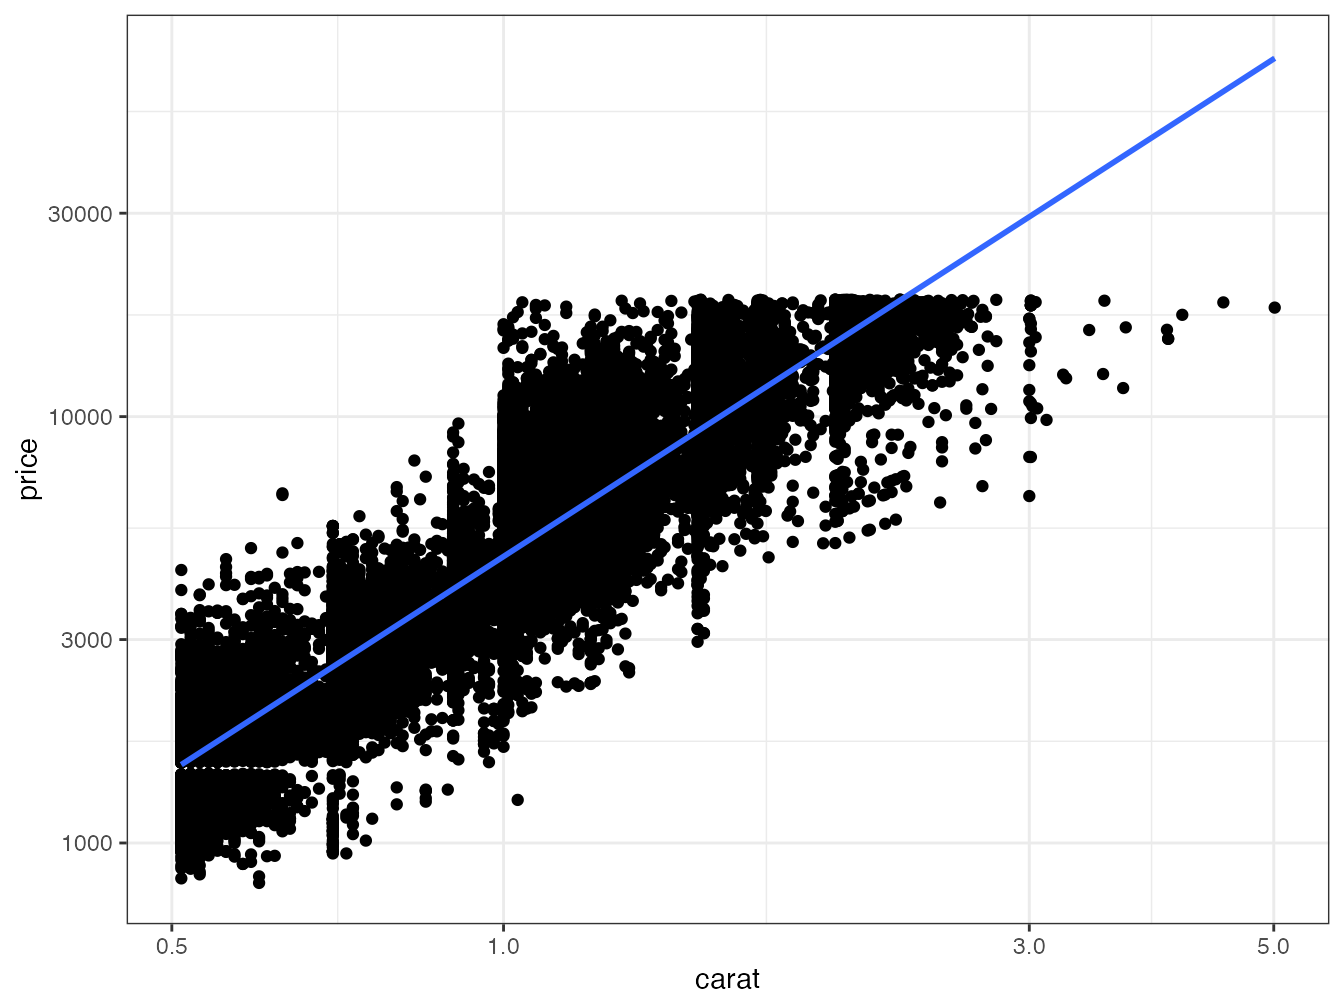
\includegraphics[width=0.8\linewidth]{travailleR_files/figure-latex/diamonds-1} 

}

\caption{Prix des diamants en fonction de leur poids. Démonstration du code de \textbf{ggplot2} combiné au traitement de données du tidyverse.}\label{fig:diamonds}
\end{figure}

\normalsize

Dans cette figure, deux géométries (nuage de points et régression linéaire) partagent la même esthétique (prix en fonction du poids en carats) qui est donc déclarée en amont, dans la fonction \texttt{ggplot()}.

Le tidyverse est documenté en détail dans \textcite{Wickham2016} et \textbf{ggplot2} dans \textcite{Wickham2017}.

\section{Environnements}\label{sec:environnements}

Les objets de R, données et fonctions, sont nommés.
Comme R est modulaire, avec la possibilité de lui ajouter un nombre indéterminé de packages, il est très probable que des conflits de nom apparaissent.
Pour les régler, R dispose d'un système rigoureux de précédence des noms: le code s'exécute dans un environnement défini, héritant d'environnements parents.

\subsection{Organisation}\label{organisation}

R démarre dans un environnement vide.
Chaque package chargé crée un environnement fils pour former une pile des environnements, dont chaque nouvel élément est appelé \enquote{fils} du précédent, qui est son \enquote{parent}.

La console se trouve dans l'environnement global, fils du dernier package chargé.

\scriptsize

\begin{Shaded}
\begin{Highlighting}[]
\FunctionTok{search}\NormalTok{()}
\end{Highlighting}
\end{Shaded}

\begin{verbatim}
##  [1] ".GlobalEnv"        "package:R6"       
##  [3] "package:entropart" "package:lubridate"
##  [5] "package:forcats"   "package:stringr"  
##  [7] "package:dplyr"     "package:purrr"    
##  [9] "package:readr"     "package:tidyr"    
## [11] "package:tibble"    "package:ggplot2"  
## [13] "package:tidyverse" "package:stats"    
## [15] "package:graphics"  "package:grDevices"
## [17] "package:utils"     "package:datasets" 
## [19] "package:methods"   "Autoloads"        
## [21] "package:base"
\end{verbatim}

\normalsize

Le code d'une fonction appelée de la console s'exécute dans un environnement fils de l'environnement global:

\scriptsize

\begin{Shaded}
\begin{Highlighting}[]
\CommentTok{\# Environnement actuel}
\FunctionTok{environment}\NormalTok{()}
\end{Highlighting}
\end{Shaded}

\begin{verbatim}
## <environment: R_GlobalEnv>
\end{verbatim}

\begin{Shaded}
\begin{Highlighting}[]
\CommentTok{\# La fonction f affiche son environnement}
\NormalTok{f }\OtherTok{\textless{}{-}} \ControlFlowTok{function}\NormalTok{() }\FunctionTok{environment}\NormalTok{()}
\CommentTok{\# Affichage de l\textquotesingle{}environnement de la fonction}
\FunctionTok{f}\NormalTok{()}
\end{Highlighting}
\end{Shaded}

\begin{verbatim}
## <environment: 0x137bca550>
\end{verbatim}

\begin{Shaded}
\begin{Highlighting}[]
\CommentTok{\# Environnement parent de celui de la fonction}
\FunctionTok{parent.env}\NormalTok{(}\FunctionTok{f}\NormalTok{())}
\end{Highlighting}
\end{Shaded}

\begin{verbatim}
## <environment: R_GlobalEnv>
\end{verbatim}

\normalsize

\subsection{Recherche}\label{recherche}

La recherche des objets commence dans l'environnement local.
S'il n'est pas trouvé, il est cherché dans l'environnement parent, puis dans le parent du parent, jusqu'à l'épuisement des environnements qui génère une erreur indiquant que l'objet n'a pas été trouvé.

Exemple:

\scriptsize

\begin{Shaded}
\begin{Highlighting}[]
\CommentTok{\# Variable q définie dans l\textquotesingle{}environnement global}
\NormalTok{q }\OtherTok{\textless{}{-}} \StringTok{"GlobalEnv"}
\CommentTok{\# Fonction définissant q dans son environnement}
\NormalTok{qLocalFonction }\OtherTok{\textless{}{-}} \ControlFlowTok{function}\NormalTok{() \{}
\NormalTok{  q }\OtherTok{\textless{}{-}} \StringTok{"Fonction"}
  \FunctionTok{return}\NormalTok{(q)}
\NormalTok{\}}
\CommentTok{\# La variable locale est retournée}
\FunctionTok{qLocalFonction}\NormalTok{()}
\end{Highlighting}
\end{Shaded}

\begin{verbatim}
## [1] "Fonction"
\end{verbatim}

\begin{Shaded}
\begin{Highlighting}[]
\CommentTok{\# Fonction (mal écrite) utilisant une variable qu\textquotesingle{}elle ne définit pas}
\NormalTok{qGlobalEnv }\OtherTok{\textless{}{-}} \ControlFlowTok{function}\NormalTok{() \{}
   \FunctionTok{return}\NormalTok{(q)}
\NormalTok{\}}
\CommentTok{\# La variable de l\textquotesingle{}environnement global est retournée}
\FunctionTok{qGlobalEnv}\NormalTok{()}
\end{Highlighting}
\end{Shaded}

\begin{verbatim}
## [1] "GlobalEnv"
\end{verbatim}

\begin{Shaded}
\begin{Highlighting}[]
\CommentTok{\# Suppression de cette variable}
\FunctionTok{rm}\NormalTok{(q)}
\CommentTok{\# La fonction base::q est retournée}
\FunctionTok{qGlobalEnv}\NormalTok{()}
\end{Highlighting}
\end{Shaded}

\begin{verbatim}
## function (save = "default", status = 0, runLast = TRUE) 
## .Internal(quit(save, status, runLast))
## <bytecode: 0x135be0998>
## <environment: namespace:base>
\end{verbatim}

\normalsize

La variable \texttt{q} est définie dans l'environnement global.
La fonction \texttt{qLocalFonction} définit sa propre variable \texttt{q}.
L'appel de la fonction retourne la valeur locale de la fonction parce qu'elle se trouve dans l'environnement de la fonction.

La fonction \texttt{qGlobalEnv} retourne la variable \texttt{q} qu'elle ne définit pas localement.
Elle la recherche donc dans son environnement parent et trouve la variable définie dans l'environnement global.
En supprimant la variable de l'environnement global par \texttt{rm(q)}, la fonction \texttt{qGlobalEnv()} parcourt la pile des environnements jusqu'à trouver un objet nommé \texttt{q} dans le package \textbf{base}, qui est la fonction permettant de quitter R.
Elle aurait pu trouver un autre objet si un package contenant un objet \texttt{q} avait été chargé.

Pour éviter ce comportement erratique, une fonction ne doit \emph{jamais} appeler un objet non défini dans son propre environnement.

\subsection{Espaces de nom des packages}\label{espaces-de-nom-des-packages}

Il est temps de définir précisément ce que les packages rendent visible.
Les packages contiennent des objets (fonctions et données) qu'ils \emph{exportent} ou non.
Ils sont habituellement appelés par la fonction \texttt{library()} qui effectue deux opérations:

\begin{itemize}
\tightlist
\item
  elle \emph{charge} le package en mémoire, ce qui permet d'accéder à tous ses objets avec la syntaxe \texttt{package::objet} pour les objets exportés et \texttt{package:::objet} pour ceux qui ne le sont pas;
\item
  elle \emph{attache} ensuite le package, ce qui place son environnement en haut de la pile.
\end{itemize}

Il est possible de détacher un package avec la fonction \texttt{unloadNamespace()} pour le retirer de la pile des environnements.
Exemple:

\scriptsize

\begin{Shaded}
\begin{Highlighting}[]
\CommentTok{\# entropart chargé et attaché}
\FunctionTok{library}\NormalTok{(}\StringTok{"entropart"}\NormalTok{)}
\CommentTok{\# Est{-}il attaché ?}
\FunctionTok{isNamespaceLoaded}\NormalTok{(}\StringTok{"entropart"}\NormalTok{)}
\end{Highlighting}
\end{Shaded}

\begin{verbatim}
## [1] TRUE
\end{verbatim}

\begin{Shaded}
\begin{Highlighting}[]
\CommentTok{\# Pile des environnements}
\FunctionTok{search}\NormalTok{()}
\end{Highlighting}
\end{Shaded}

\begin{verbatim}
##  [1] ".GlobalEnv"        "package:R6"       
##  [3] "package:entropart" "package:lubridate"
##  [5] "package:forcats"   "package:stringr"  
##  [7] "package:dplyr"     "package:purrr"    
##  [9] "package:readr"     "package:tidyr"    
## [11] "package:tibble"    "package:ggplot2"  
## [13] "package:tidyverse" "package:stats"    
## [15] "package:graphics"  "package:grDevices"
## [17] "package:utils"     "package:datasets" 
## [19] "package:methods"   "Autoloads"        
## [21] "package:base"
\end{verbatim}

\begin{Shaded}
\begin{Highlighting}[]
\CommentTok{\# Diversity(), une fonction exportée par entropart est trouvée}
\FunctionTok{Diversity}\NormalTok{(}\DecValTok{1}\NormalTok{, }\AttributeTok{CheckArguments =} \ConstantTok{FALSE}\NormalTok{)}
\end{Highlighting}
\end{Shaded}

\begin{verbatim}
## None 
##    1
\end{verbatim}

\begin{Shaded}
\begin{Highlighting}[]
\CommentTok{\# Détacher et décharger entropart}
\FunctionTok{unloadNamespace}\NormalTok{(}\StringTok{"entropart"}\NormalTok{)}
\CommentTok{\# Est{-}il attaché ?}
\FunctionTok{isNamespaceLoaded}\NormalTok{(}\StringTok{"entropart"}\NormalTok{)}
\end{Highlighting}
\end{Shaded}

\begin{verbatim}
## [1] FALSE
\end{verbatim}

\begin{Shaded}
\begin{Highlighting}[]
\CommentTok{\# Pile des environnements, sans entropart}
\FunctionTok{search}\NormalTok{()}
\end{Highlighting}
\end{Shaded}

\begin{verbatim}
##  [1] ".GlobalEnv"        "package:R6"       
##  [3] "package:lubridate" "package:forcats"  
##  [5] "package:stringr"   "package:dplyr"    
##  [7] "package:purrr"     "package:readr"    
##  [9] "package:tidyr"     "package:tibble"   
## [11] "package:ggplot2"   "package:tidyverse"
## [13] "package:stats"     "package:graphics" 
## [15] "package:grDevices" "package:utils"    
## [17] "package:datasets"  "package:methods"  
## [19] "Autoloads"         "package:base"
\end{verbatim}

\begin{Shaded}
\begin{Highlighting}[]
\CommentTok{\# Diversity() est introuvable}
\FunctionTok{tryCatch}\NormalTok{(}\FunctionTok{Diversity}\NormalTok{(}\DecValTok{1}\NormalTok{), }\AttributeTok{error =} \ControlFlowTok{function}\NormalTok{(e) }\FunctionTok{print}\NormalTok{(e))}
\end{Highlighting}
\end{Shaded}

\begin{verbatim}
## <simpleError in Diversity(1): could not find function "Diversity">
\end{verbatim}

\begin{Shaded}
\begin{Highlighting}[]
\CommentTok{\# mais peut être appelée avec son nom complet}
\NormalTok{entropart}\SpecialCharTok{::}\FunctionTok{Diversity}\NormalTok{(}\DecValTok{1}\NormalTok{, }\AttributeTok{CheckArguments =} \ConstantTok{FALSE}\NormalTok{)}
\end{Highlighting}
\end{Shaded}

\begin{verbatim}
## None 
##    1
\end{verbatim}

\normalsize

L'appel de \texttt{entropart::Diversity()} charge le package (c'est-à-dire, exécute implicitement \texttt{loadNamespace("entropart")}) mais ne l'attache pas.

En pratique, il faut limiter le nombre de package attachés pour limiter le risque d'appeler une fonction non désirée, homonyme de la fonction recherchée.
Dans les cas critiques, il faut utiliser le nom complet de la fonction: \texttt{package::fonction()}.

Un problème fréquent concerne la fonction \texttt{filter()} de \textbf{dplyr} homonyme de celle de \textbf{stats}.
Le package \textbf{stats} est habituellement chargé avant \textbf{dplyr}, un package du tidyverse.
\texttt{stats::filter()} doit donc être appelée explicitement.

Cependant, le package \textbf{dplyr} ou \textbf{tidyverse} (qui attache tous les packages du tidyverse) peut être chargé systématiquement en créant un fichier \texttt{.RProfile} à la racine du projet contenant la commande:

\scriptsize

\begin{Shaded}
\begin{Highlighting}[]
\FunctionTok{library}\NormalTok{(}\StringTok{"tidyverse"}\NormalTok{)}
\end{Highlighting}
\end{Shaded}

\normalsize

Dans ce cas, \textbf{dplyr} est chargé \emph{avant} \textbf{stats} et c'est sa fonction qui est inaccessible.

\section{Mesure du temps d'exécution}\label{mesure-du-temps-dexuxe9cution}

Le temps d'exécution d'un code long peut être mesuré très simplement par la commande \texttt{system.time}.
Pour des temps d'exécution très courts, il est nécessaire de répéter la mesure: c'est l'objet du package \textbf{microbenchmark}.

\subsection{system.time}\label{system.time}

La fonction retourne le temps d'exécution du code.

\scriptsize

\begin{Shaded}
\begin{Highlighting}[]
\CommentTok{\# Ecart absolu moyen de 1000 valeurs dans une loi uniforme, répété 100 fois}
\FunctionTok{system.time}\NormalTok{(}\ControlFlowTok{for}\NormalTok{ (i }\ControlFlowTok{in} \DecValTok{1}\SpecialCharTok{:}\DecValTok{100}\NormalTok{) }\FunctionTok{mad}\NormalTok{(}\FunctionTok{runif}\NormalTok{(}\DecValTok{1000}\NormalTok{)))}
\end{Highlighting}
\end{Shaded}

\begin{verbatim}
##    user  system elapsed 
##   0.007   0.000   0.007
\end{verbatim}

\normalsize

\subsection{microbenchmark}\label{microbenchmark}

Le package \textbf{microbenchmark} est le plus avancé.

L'objectif est de comparer la vitesse du calcul du carré d'un vecteur (ou d'un nombre) en le multipliant par lui-même (\(x \times x\)) ou en l'élevant à la puissance 2 (\(x^2\)).

\scriptsize

\begin{Shaded}
\begin{Highlighting}[]
\NormalTok{f1 }\OtherTok{\textless{}{-}} \ControlFlowTok{function}\NormalTok{(x) x}\SpecialCharTok{*}\NormalTok{x}
\NormalTok{f2 }\OtherTok{\textless{}{-}} \ControlFlowTok{function}\NormalTok{(x) x}\SpecialCharTok{\^{}}\DecValTok{2}
\NormalTok{f3 }\OtherTok{\textless{}{-}} \ControlFlowTok{function}\NormalTok{(x) x}\SpecialCharTok{\^{}}\FloatTok{2.1}
\NormalTok{f4 }\OtherTok{\textless{}{-}} \ControlFlowTok{function}\NormalTok{(x) x}\SpecialCharTok{\^{}}\DecValTok{3}
\CommentTok{\# Initialisation}
\NormalTok{X }\OtherTok{\textless{}{-}} \FunctionTok{rnorm}\NormalTok{(}\DecValTok{10000}\NormalTok{)}
\CommentTok{\# Test}
\FunctionTok{library}\NormalTok{(}\StringTok{"microbenchmark"}\NormalTok{)}
\NormalTok{(mb }\OtherTok{\textless{}{-}} \FunctionTok{microbenchmark}\NormalTok{(}\FunctionTok{f1}\NormalTok{(X), }\FunctionTok{f2}\NormalTok{(X), }\FunctionTok{f3}\NormalTok{(X), }\FunctionTok{f4}\NormalTok{(X)))}
\end{Highlighting}
\end{Shaded}

\begin{verbatim}
## Unit: microseconds
##   expr     min       lq      mean  median       uq     max
##  f1(X)   1.640   2.0090   8.18852   2.911   6.9495 342.309
##  f2(X)   3.895   4.1205  10.51363   5.781   9.1635 341.817
##  f3(X)  93.480  98.6255 108.44418 105.370 109.5930 453.665
##  f4(X) 123.533 126.8745 140.03427 135.669 141.5525 592.901
##  neval
##    100
##    100
##    100
##    100
\end{verbatim}

\normalsize

Le tableau retourné contient les temps minimum, médian, moyen, max et les premiers et troisièmes quartiles, ainsi que le nombre de répétitions.
La valeur médiane est à comparer.
Le nombre de répétition est par défaut de 100, à moduler (argument \texttt{times}) en fonction de la complexité du calcul.

Le résultat du test, un objet de type \texttt{microbenchmark}, est un tableau brut des temps d'exécution.
L'analyse statistique est faite par les méthodes \texttt{print} et \texttt{summary}.
Pour choisir les colonnes à afficher, utiliser la syntaxe suivante:

\scriptsize

\begin{Shaded}
\begin{Highlighting}[]
\FunctionTok{summary}\NormalTok{(mb)[, }\FunctionTok{c}\NormalTok{(}\StringTok{"expr"}\NormalTok{, }\StringTok{"median"}\NormalTok{)]}
\end{Highlighting}
\end{Shaded}

\begin{verbatim}
##    expr  median
## 1 f1(X)   2.911
## 2 f2(X)   5.781
## 3 f3(X) 105.370
## 4 f4(X) 135.669
\end{verbatim}

\normalsize

Pour faire des calculs sur ces résultats, il faut les stocker dans une variable.
Pour empêcher l'affichage dans la console, la solution la plus simple est d'utiliser la fonction \texttt{capture.output} en affectant son résultat à une variable.

\scriptsize

\begin{Shaded}
\begin{Highlighting}[]
\NormalTok{dummy }\OtherTok{\textless{}{-}} \FunctionTok{capture.output}\NormalTok{(mbs }\OtherTok{\textless{}{-}} \FunctionTok{summary}\NormalTok{(mb))}
\end{Highlighting}
\end{Shaded}

\normalsize

Le test précédent est affiché à nouveau.

\scriptsize

\begin{Shaded}
\begin{Highlighting}[]
\FunctionTok{summary}\NormalTok{(mb)[, }\FunctionTok{c}\NormalTok{(}\StringTok{"expr"}\NormalTok{, }\StringTok{"median"}\NormalTok{)]}
\end{Highlighting}
\end{Shaded}

\begin{verbatim}
##    expr  median
## 1 f1(X)   2.911
## 2 f2(X)   5.781
## 3 f3(X) 105.370
## 4 f4(X) 135.669
\end{verbatim}

\normalsize

Le temps de calcul est à peu près identique entre \(x \times x\) et \(x^2\).
Le calcul de puissance est nettement plus long, surtout si la puissance n'est pas entière, parce qu'il nécessite un calcul de logarithme.
Le calcul de la puissance 2 est donc optimisé par R pour éviter l'usage du log.

Deux représentations graphiques sont disponibles: les violons représentent la densité de probabilité du temps d'exécution; les boîtes à moustache sont classiques.

\scriptsize

\begin{Shaded}
\begin{Highlighting}[]
\FunctionTok{library}\NormalTok{(}\StringTok{"ggplot2"}\NormalTok{)}
\FunctionTok{autoplot}\NormalTok{(mb)}
\end{Highlighting}
\end{Shaded}

\begin{center}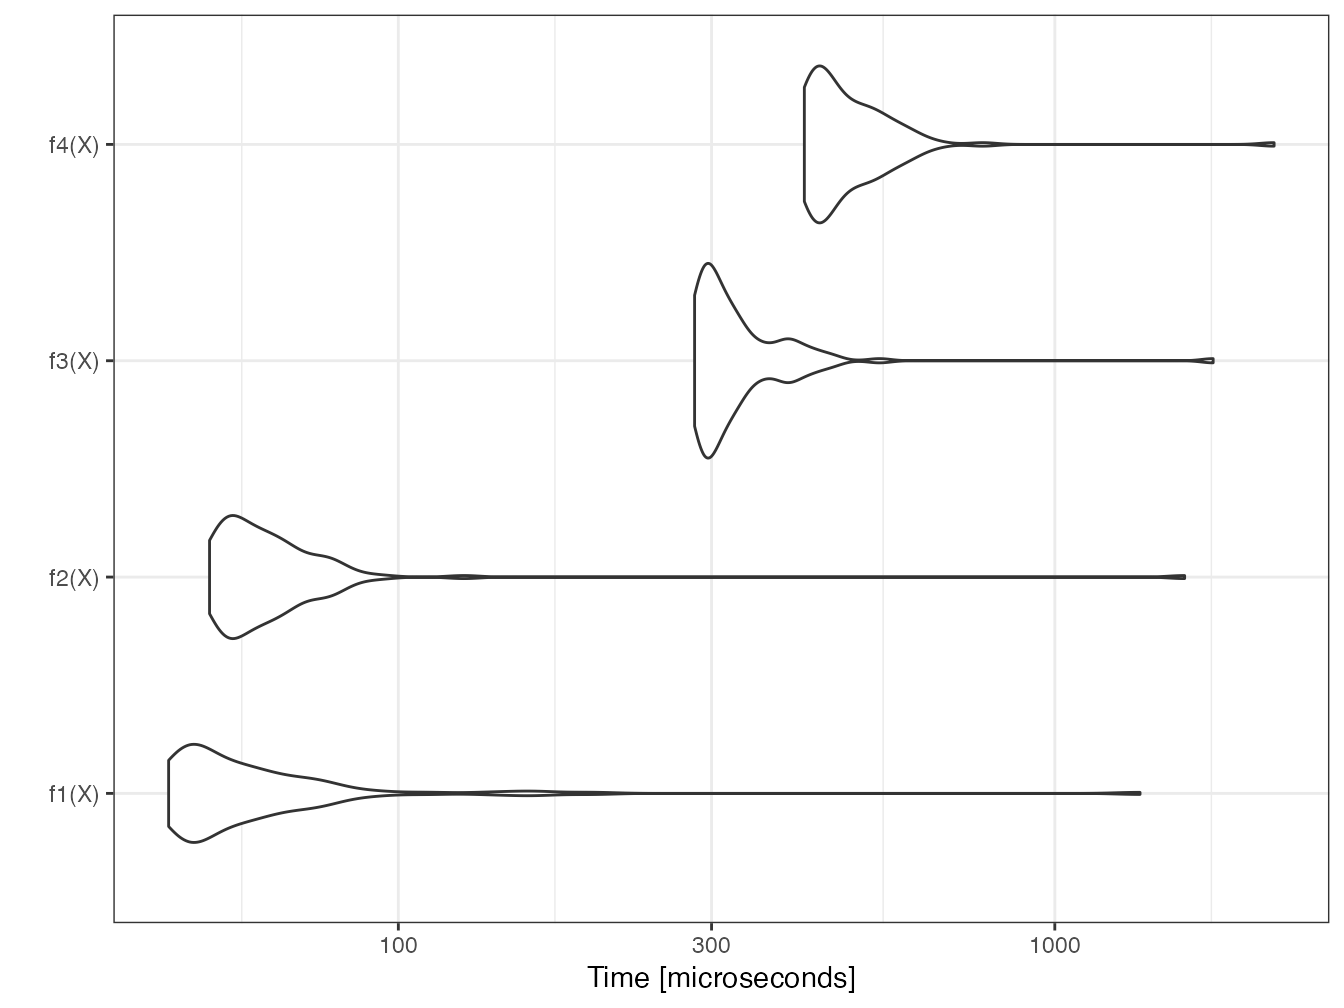
\includegraphics[width=0.8\linewidth]{travailleR_files/figure-latex/boxplot-1} \end{center}

\begin{Shaded}
\begin{Highlighting}[]
\FunctionTok{boxplot}\NormalTok{(mb)}
\end{Highlighting}
\end{Shaded}

\begin{center}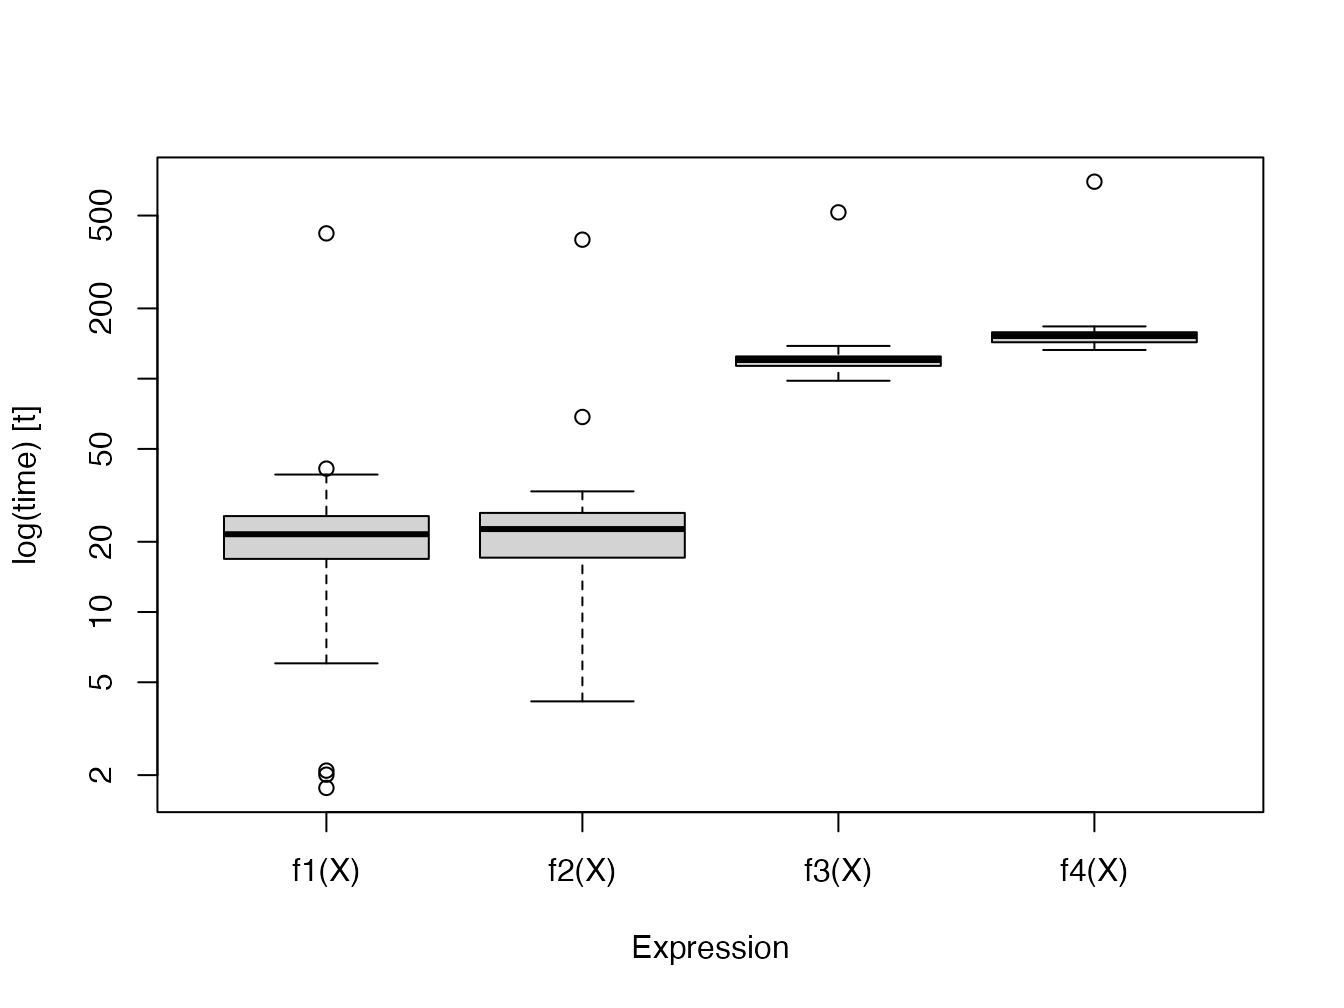
\includegraphics[width=0.8\linewidth]{travailleR_files/figure-latex/boxplot-2} \end{center}

\normalsize

\subsection{Profilage}\label{profilage}

\textbf{profvis} est l'outil de profilage de RStudio.

Il permet de suivre le temps d'exécution de chaque ligne de code et la mémoire utilisée.
L'objectif est de détecter les portions de code lentes, à améliorer.

\scriptsize

\begin{Shaded}
\begin{Highlighting}[]
\FunctionTok{library}\NormalTok{(profvis)}
\NormalTok{p }\OtherTok{\textless{}{-}} \FunctionTok{profvis}\NormalTok{(\{}
  \CommentTok{\# Calculs de cosinus }
  \FunctionTok{cos}\NormalTok{(}\FunctionTok{runif}\NormalTok{(}\DecValTok{10}\SpecialCharTok{\^{}}\DecValTok{7}\NormalTok{))}
  \CommentTok{\# 1/2 seconde de pause}
  \FunctionTok{pause}\NormalTok{(}\DecValTok{1} \SpecialCharTok{/} \DecValTok{2}\NormalTok{)}
\NormalTok{  \})}
\NormalTok{htmlwidgets}\SpecialCharTok{::}\FunctionTok{saveWidget}\NormalTok{(p, }\StringTok{"docs/profile.html"}\NormalTok{)}
\end{Highlighting}
\end{Shaded}

\normalsize

Le résultat est un fichier HTML contenant le rapport de profilage\footnote{\url{https://EricMarcon.github.io/travailleR/profile.html}}.
On peut observer que le temps de tirage des nombres aléatoires est similaire à celui du calcul des cosinus.

Lire la documentation complète\footnote{\url{https://rstudio.github.io/profvis/}} sur le site de RStudio.

\section{Boucles}\label{boucles}

Le cas le plus fréquent de code long à exécuter est celui des boucles: le même code est répété un grand nombre de fois.

\subsection{Fonctions vectorielles}\label{fonctions-vectorielles}

La plupart des fonctions de R sont vectorielles: les boucles sont traitées de façon interne, extrêmement rapide.
Il faut donc raisonner en termes de vecteurs plutôt que de scalaires.

\scriptsize

\begin{Shaded}
\begin{Highlighting}[]
\CommentTok{\# Tirage de deux vecteurs de trois nombres aléatoires entre 0 et 1}
\NormalTok{x1 }\OtherTok{\textless{}{-}} \FunctionTok{runif}\NormalTok{(}\DecValTok{3}\NormalTok{)}
\NormalTok{x2 }\OtherTok{\textless{}{-}} \FunctionTok{runif}\NormalTok{(}\DecValTok{3}\NormalTok{)}
\CommentTok{\# Racine carrée des trois nombres de x1}
\FunctionTok{sqrt}\NormalTok{(x1)}
\end{Highlighting}
\end{Shaded}

\begin{verbatim}
## [1] 0.9427738 0.8665204 0.4586981
\end{verbatim}

\begin{Shaded}
\begin{Highlighting}[]
\CommentTok{\# Sommes respective des trois nombres de x1 et x2}
\NormalTok{x1 }\SpecialCharTok{+}\NormalTok{ x2}
\end{Highlighting}
\end{Shaded}

\begin{verbatim}
## [1] 1.6262539 1.6881583 0.9063973
\end{verbatim}

\normalsize

Il faut aussi écrire des fonctions vectorielles sur leur premier argument.
La fonction \texttt{lnq} du package \textbf{entropart} retourne le logarithme déformé d'ordre \(q\) d'un nombre \(x\).

\scriptsize

\begin{Shaded}
\begin{Highlighting}[]
\CommentTok{\# Code de la fonction}
\NormalTok{entropart}\SpecialCharTok{::}\NormalTok{lnq}
\end{Highlighting}
\end{Shaded}

\begin{verbatim}
## function (x, q) 
## {
##     if (q == 1) {
##         return(log(x))
##     }
##     else {
##         Log <- (x^(1 - q) - 1)/(1 - q)
##         Log[x < 0] <- NA
##         return(Log)
##     }
## }
## <bytecode: 0x14453a008>
## <environment: namespace:entropart>
\end{verbatim}

\normalsize

Pour qu'une fonction soit vectorielle, chaque ligne de son code doit permettre que le premier argument soit traité comme un vecteur.
Ici: \texttt{log(x)} et \texttt{x\^{}} sont une fonction et un opérateur vectoriels et la condition \texttt{{[}x\ \textless{}\ 0{]}} retourne aussi un vecteur.

\subsection{lapply}\label{lapply}

Les codes qui ne peuvent pas être écrits comme une fonction vectorielle nécessitent des boucles.

\texttt{lapply()} applique une fonction à chaque élément d'une liste.
Elle est déclinée sous plusieurs versions:

\begin{itemize}
\tightlist
\item
  \texttt{lapply()} renvoie une liste (économise le temps de leur réorganisation dans un tableau);
\item
  \texttt{sapply()} renvoie un dataframe en rassemblant les listes par \texttt{simplify2array()};
\item
  \texttt{vapply()} est presque identique mais demande que le type de données du résultat soit fourni.
\end{itemize}

\scriptsize

\begin{Shaded}
\begin{Highlighting}[]
\CommentTok{\# Tirage de 1000 valeurs dans une loi uniforme}
\NormalTok{x1 }\OtherTok{\textless{}{-}} \FunctionTok{runif}\NormalTok{(}\DecValTok{1000}\NormalTok{)}
\CommentTok{\# La racine carrée peut être calculée pour le vecteur ou chaque valeur }
\FunctionTok{identical}\NormalTok{(}\FunctionTok{sqrt}\NormalTok{(x1), }\FunctionTok{sapply}\NormalTok{(x1, }\AttributeTok{FUN =}\NormalTok{ sqrt))}
\end{Highlighting}
\end{Shaded}

\begin{verbatim}
## [1] TRUE
\end{verbatim}

\begin{Shaded}
\begin{Highlighting}[]
\NormalTok{mb }\OtherTok{\textless{}{-}} \FunctionTok{microbenchmark}\NormalTok{(}
  \FunctionTok{sqrt}\NormalTok{(x1), }
  \FunctionTok{lapply}\NormalTok{(x1, }\AttributeTok{FUN =}\NormalTok{ sqrt), }
  \FunctionTok{sapply}\NormalTok{(x1, }\AttributeTok{FUN =}\NormalTok{ sqrt), }
  \FunctionTok{vapply}\NormalTok{(x1, }\AttributeTok{FUN =}\NormalTok{ sqrt, }\AttributeTok{FUN.VALUE =} \DecValTok{0}\NormalTok{)}
\NormalTok{)}
\FunctionTok{summary}\NormalTok{(mb)[, }\FunctionTok{c}\NormalTok{(}\StringTok{"expr"}\NormalTok{, }\StringTok{"median"}\NormalTok{)]}
\end{Highlighting}
\end{Shaded}

\begin{verbatim}
##                                    expr   median
## 1                              sqrt(x1)   1.5170
## 2                lapply(x1, FUN = sqrt) 135.8535
## 3                sapply(x1, FUN = sqrt) 165.4555
## 4 vapply(x1, FUN = sqrt, FUN.VALUE = 0) 133.2910
\end{verbatim}

\normalsize

\texttt{lapply()} est beaucoup plus lent qu'une fonction vectorielle.
\texttt{sapply()} nécessite plus de temps pour \texttt{simplify2array()}, qui doit détecter comment rassembler les résultats.
Enfin, \texttt{vapply()} économise le temps de détermination du type de données du résultat et permet d'accélérer le calcul avec peu d'efforts.

\subsection{Boucles for}\label{boucles-for}

Les boucles sont gérées par la fonction \texttt{for}.
Elles ont la réputation d'être lentes dans R parce que le code à l'intérieur de la boucle doit être interprété à chaque exécution.
Ce n'est plus le cas depuis la version 3.5 de R: les boucles sont compilées systématiquement avant leur exécution.
Le comportement du compilateur \enquote{juste à temps} est défini par la fonction \texttt{enableJIT}.
Le niveau par défaut est 3: les fonctions sont toutes compilées, et les boucles dans le code aussi.

Pour évaluer le gain de performance, le code suivant supprime toute compilation automatique, et compare la même boucle compilée ou non.

\scriptsize

\begin{Shaded}
\begin{Highlighting}[]
\FunctionTok{library}\NormalTok{(}\StringTok{"compiler"}\NormalTok{)}
\CommentTok{\# Pas de compilation automatique}
\FunctionTok{enableJIT}\NormalTok{(}\AttributeTok{level =} \DecValTok{0}\NormalTok{)}
\end{Highlighting}
\end{Shaded}

\begin{verbatim}
## [1] 3
\end{verbatim}

\begin{Shaded}
\begin{Highlighting}[]
\CommentTok{\# Boucle pour calculer la racine carrée d\textquotesingle{}un vecteur}
\NormalTok{Boucle }\OtherTok{\textless{}{-}} \ControlFlowTok{function}\NormalTok{(x) \{}
  \CommentTok{\# Initialisation du vecteur de résultat, indispensable}
\NormalTok{  Racine }\OtherTok{\textless{}{-}} \FunctionTok{vector}\NormalTok{(}\StringTok{"numeric"}\NormalTok{, }\AttributeTok{length =} \FunctionTok{length}\NormalTok{(x))}
  \CommentTok{\# Boucle}
  \ControlFlowTok{for}\NormalTok{ (i }\ControlFlowTok{in} \DecValTok{1}\SpecialCharTok{:}\FunctionTok{length}\NormalTok{(x)) Racine[i] }\OtherTok{\textless{}{-}} \FunctionTok{sqrt}\NormalTok{(x[i])}
  \FunctionTok{return}\NormalTok{(Racine)}
\NormalTok{\}}
\CommentTok{\# Version compilée}
\NormalTok{Boucle2 }\OtherTok{\textless{}{-}} \FunctionTok{cmpfun}\NormalTok{(Boucle)}
\CommentTok{\# Comparaison}
\NormalTok{mb }\OtherTok{\textless{}{-}} \FunctionTok{microbenchmark}\NormalTok{(}\FunctionTok{Boucle}\NormalTok{(x1), }\FunctionTok{Boucle2}\NormalTok{(x1))}
\NormalTok{(mbs }\OtherTok{\textless{}{-}} \FunctionTok{summary}\NormalTok{(mb)[, }\FunctionTok{c}\NormalTok{(}\StringTok{"expr"}\NormalTok{, }\StringTok{"median"}\NormalTok{)])}
\end{Highlighting}
\end{Shaded}

\begin{verbatim}
##          expr   median
## 1  Boucle(x1) 369.9225
## 2 Boucle2(x1)  42.9270
\end{verbatim}

\begin{Shaded}
\begin{Highlighting}[]
\CommentTok{\# Compilation automatique par défaut depuis la version 3.5}
\FunctionTok{enableJIT}\NormalTok{(}\AttributeTok{level =} \DecValTok{3}\NormalTok{)}
\end{Highlighting}
\end{Shaded}

\begin{verbatim}
## [1] 0
\end{verbatim}

\normalsize

Le gain est considérable: de 1 à \texttt{9}.

Les boucles for sont maintenant nettement plus rapides que \texttt{vapply}.

\scriptsize

\begin{Shaded}
\begin{Highlighting}[]
\CommentTok{\# Test}
\NormalTok{mb }\OtherTok{\textless{}{-}} \FunctionTok{microbenchmark}\NormalTok{(}\FunctionTok{vapply}\NormalTok{(x1, }\AttributeTok{FUN =}\NormalTok{ sqrt, }\DecValTok{0}\NormalTok{), }\FunctionTok{Boucle}\NormalTok{(x1))}
\FunctionTok{summary}\NormalTok{(mb)[, }\FunctionTok{c}\NormalTok{(}\StringTok{"expr"}\NormalTok{, }\StringTok{"median"}\NormalTok{)]}
\end{Highlighting}
\end{Shaded}

\begin{verbatim}
##                        expr   median
## 1 vapply(x1, FUN = sqrt, 0) 133.6805
## 2                Boucle(x1)  41.8815
\end{verbatim}

\normalsize

Attention, le test de performance peut être trompeur:

\scriptsize

\begin{Shaded}
\begin{Highlighting}[]
\CommentTok{\# Préparation du vecteur de résultat}
\NormalTok{Racine }\OtherTok{\textless{}{-}} \FunctionTok{vector}\NormalTok{(}\StringTok{"numeric"}\NormalTok{, }\AttributeTok{length =} \FunctionTok{length}\NormalTok{(x1))}
\CommentTok{\# Test}
\NormalTok{mb }\OtherTok{\textless{}{-}} \FunctionTok{microbenchmark}\NormalTok{(}
  \FunctionTok{vapply}\NormalTok{(x1, }\AttributeTok{FUN =}\NormalTok{ sqrt, }\DecValTok{0}\NormalTok{), }
  \ControlFlowTok{for}\NormalTok{ (i }\ControlFlowTok{in} \DecValTok{1}\SpecialCharTok{:}\FunctionTok{length}\NormalTok{(x1)) Racine[i] }\OtherTok{\textless{}{-}} \FunctionTok{sqrt}\NormalTok{(x1[i])}
\NormalTok{)}
\FunctionTok{summary}\NormalTok{(mb)[, }\FunctionTok{c}\NormalTok{(}\StringTok{"expr"}\NormalTok{, }\StringTok{"median"}\NormalTok{)]}
\end{Highlighting}
\end{Shaded}

\begin{verbatim}
##                                               expr
## 1                        vapply(x1, FUN = sqrt, 0)
## 2 for (i in 1:length(x1)) Racine[i] <- sqrt(x1[i])
##      median
## 1  138.7645
## 2 1140.5175
\end{verbatim}

\normalsize

Dans ce code, la boucle for n'est pas compilée donc elle est beaucoup plus lente que dans le cadre normal de son utilisation (dans une fonction ou au niveau supérieur du code).

Les boucles longues permettent un suivi de leur progression par une barre de texte, ce qui est un autre avantage.
La fonction suivante exécute des pauses d'un dixième de seconde pendant le temps passé en paramètre (en secondes).

\scriptsize

\begin{Shaded}
\begin{Highlighting}[]
\NormalTok{BoucleSuivie }\OtherTok{\textless{}{-}} \ControlFlowTok{function}\NormalTok{(}\AttributeTok{duree =} \DecValTok{1}\NormalTok{) \{}
  \CommentTok{\# Barre de progression}
\NormalTok{  pgb }\OtherTok{\textless{}{-}} \FunctionTok{txtProgressBar}\NormalTok{(}\AttributeTok{min =} \DecValTok{0}\NormalTok{, }\AttributeTok{max =}\NormalTok{ duree }\SpecialCharTok{*} \DecValTok{10}\NormalTok{)}
  \CommentTok{\# Boucle}
  \ControlFlowTok{for}\NormalTok{ (i }\ControlFlowTok{in} \DecValTok{1}\SpecialCharTok{:}\NormalTok{(duree }\SpecialCharTok{*} \DecValTok{10}\NormalTok{)) \{}
    \CommentTok{\# Pause d\textquotesingle{}un dixième de seconde}
    \FunctionTok{Sys.sleep}\NormalTok{(}\DecValTok{1} \SpecialCharTok{/} \DecValTok{10}\NormalTok{)}
    \CommentTok{\# Suivi de la progression}
    \FunctionTok{setTxtProgressBar}\NormalTok{(pgb, i)}
\NormalTok{  \}}
\NormalTok{\}}
\FunctionTok{BoucleSuivie}\NormalTok{()}
\end{Highlighting}
\end{Shaded}

\begin{verbatim}
## ============================================================
\end{verbatim}

\normalsize

\subsection{replicate}\label{replicate}

\texttt{replicate()} répète une instruction.

\scriptsize

\begin{Shaded}
\begin{Highlighting}[]
\FunctionTok{replicate}\NormalTok{(}\DecValTok{3}\NormalTok{, }\FunctionTok{runif}\NormalTok{(}\DecValTok{1}\NormalTok{))}
\end{Highlighting}
\end{Shaded}

\begin{verbatim}
## [1] 0.9453453 0.5262818 0.7233425
\end{verbatim}

\normalsize

Ce code est équivalent à \texttt{runif(3)}, avec des performances similaires à celles de \texttt{vapply}: de 50 à 100 fois plus lent qu'une fonction vectorielle.

\scriptsize

\begin{Shaded}
\begin{Highlighting}[]
\NormalTok{mb }\OtherTok{\textless{}{-}} \FunctionTok{microbenchmark}\NormalTok{(}\FunctionTok{replicate}\NormalTok{(}\FloatTok{1E3}\NormalTok{, }\FunctionTok{runif}\NormalTok{(}\DecValTok{1}\NormalTok{)), }\FunctionTok{runif}\NormalTok{(}\FloatTok{1E3}\NormalTok{))}
\FunctionTok{summary}\NormalTok{(mb)[, }\FunctionTok{c}\NormalTok{(}\StringTok{"expr"}\NormalTok{, }\StringTok{"median"}\NormalTok{)]}
\end{Highlighting}
\end{Shaded}

\begin{verbatim}
##                        expr  median
## 1 replicate(1000, runif(1)) 721.805
## 2               runif(1000)   6.273
\end{verbatim}

\normalsize

\subsection{Vectorize}\label{vectorize}

\texttt{Vectorize()} rend vectorielle une fonction qui ne l'est pas, par des boucles.
Ecrire plutôt les boucles.

\subsection{Statistiques marginales}\label{statistiques-marginales}

\texttt{apply} applique une fonction aux lignes ou colonnes d'un objet en deux dimensions.

\texttt{colSums} et ses semblables (\texttt{rowSums}, \texttt{colMeans}, \texttt{rowMeans}) sont optimisées.

\scriptsize

\begin{Shaded}
\begin{Highlighting}[]
\CommentTok{\# Somme des colonnes numériques du jeu de données diamonds de ggplot2}
\CommentTok{\# Boucle identique à l\textquotesingle{}action de apply(, 2, )}
\NormalTok{BoucleSomme }\OtherTok{\textless{}{-}} \ControlFlowTok{function}\NormalTok{(Table) \{}
\NormalTok{  Somme }\OtherTok{\textless{}{-}} \FunctionTok{vector}\NormalTok{(}\StringTok{"numeric"}\NormalTok{, }\AttributeTok{length =} \FunctionTok{ncol}\NormalTok{(Table))}
  \ControlFlowTok{for}\NormalTok{ (i }\ControlFlowTok{in} \DecValTok{1}\SpecialCharTok{:}\FunctionTok{ncol}\NormalTok{(Table)) Somme[i] }\OtherTok{\textless{}{-}} \FunctionTok{sum}\NormalTok{(Table[, i])}
  \FunctionTok{return}\NormalTok{(Somme)}
\NormalTok{\}}
\NormalTok{mb }\OtherTok{\textless{}{-}} \FunctionTok{microbenchmark}\NormalTok{(}
  \FunctionTok{BoucleSomme}\NormalTok{(diamonds[}\SpecialCharTok{{-}}\NormalTok{(}\DecValTok{2}\SpecialCharTok{:}\DecValTok{4}\NormalTok{)]), }
  \FunctionTok{apply}\NormalTok{(diamonds[}\SpecialCharTok{{-}}\NormalTok{(}\DecValTok{2}\SpecialCharTok{:}\DecValTok{4}\NormalTok{)], }\DecValTok{2}\NormalTok{, sum), }
  \FunctionTok{colSums}\NormalTok{(diamonds[}\SpecialCharTok{{-}}\NormalTok{(}\DecValTok{2}\SpecialCharTok{:}\DecValTok{4}\NormalTok{)])}
\NormalTok{)}
\FunctionTok{summary}\NormalTok{(mb)[, }\FunctionTok{c}\NormalTok{(}\StringTok{"expr"}\NormalTok{, }\StringTok{"median"}\NormalTok{)]}
\end{Highlighting}
\end{Shaded}

\begin{verbatim}
##                              expr   median
## 1   BoucleSomme(diamonds[-(2:4)]) 1543.342
## 2 apply(diamonds[-(2:4)], 2, sum) 3432.541
## 3       colSums(diamonds[-(2:4)]) 1172.477
\end{verbatim}

\normalsize

\texttt{apply} clarifie le code mais est plus lent que la boucle, qui est à peine plus lente que \texttt{colSums}.

\section{Code C++}\label{sec:cpp}

L'intégration de code C++ dans R est largement simplifiée par le package \textbf{Rcpp} mais reste difficile à déboguer et donc à réserver à du code très simple (pour éviter toute erreur) et répété un grand nombre de fois (pour mériter l'effort).
La préparation des données et leur vérification doivent être exécutées sous R, de même que le traitement et la présentation des résultats.

L'utilisation habituelle est l'inclusion de code C++ dans un package, mais l'utilisation hors package est possible:

\begin{itemize}
\tightlist
\item
  Le code C++ peut être inclus dans un document C++ (fichier avec l'extension \texttt{.cpp}): il est compilé par la commande \texttt{sourceCpp()} qui crée les fonctions R permettant d'appeler le code C++.
\item
  Dans un document RMarkdown, des bouts de code Rcpp peuvent être créés pour y insérer le code C++: ils sont compilés et interfacés pour R au moment du tricotage.
\end{itemize}

L'exemple suivant montre comment créer une fonction C++ pour calculer le double d'un vecteur numérique.

\scriptsize

\begin{Shaded}
\begin{Highlighting}[]
\PreprocessorTok{\#include }\ImportTok{\textless{}Rcpp.h\textgreater{}}
\KeywordTok{using} \KeywordTok{namespace}\NormalTok{ Rcpp}\OperatorTok{;}

\CommentTok{// [[Rcpp::export]]}
\NormalTok{NumericVector timesTwo}\OperatorTok{(}\NormalTok{NumericVector x}\OperatorTok{)} \OperatorTok{\{}
  \ControlFlowTok{return}\NormalTok{ x }\OperatorTok{*} \DecValTok{2}\OperatorTok{;}
\OperatorTok{\}}
\end{Highlighting}
\end{Shaded}

\normalsize

Une fonction R du même nom que la fonction C++ est maintenant disponible.

\scriptsize

\begin{Shaded}
\begin{Highlighting}[]
\FunctionTok{timesTwo}\NormalTok{(}\DecValTok{1}\SpecialCharTok{:}\DecValTok{5}\NormalTok{)}
\end{Highlighting}
\end{Shaded}

\begin{verbatim}
## [1]  2  4  6  8 10
\end{verbatim}

\normalsize

Les performances sont deux ordres de grandeur plus rapides que le code R (voir l'étude de cas, section \ref{sec:cas}).

\section{Paralléliser R}\label{sec:parallel}

Lorsque des calculs longs peuvent être découpés en tâches indépendantes, l'exécution simultanée (\emph{parallèle}) de ces tâches permet de réduire le temps de calcul total à celui de la tâche la plus longue, auquel s'ajoute le coût de la mise en place de la parallélisation (création des tâches, récupération des résultats\ldots).

Lire l'excellente introduction de Josh Errickson\footnote{\url{http://dept.stat.lsa.umich.edu/~jerrick/courses/stat701/notes/parallel.html}} qui détaille les enjeux et les contraintes de la parallélisation.

Deux mécanismes sont disponibles pour l'exécution de code en parallèle:

\begin{itemize}
\tightlist
\item
  \emph{fork}: le processus en cours d'exécution est dupliqué sur plusieurs cœurs du processeur de l'ordinateur de calcul.
  C'est la méthode la plus simple mais elle ne fonctionne pas sous Windows (limite du système d'exploitation).
\item
  \emph{socket}: un cluster est constitué, soit physiquement (un ensemble d'ordinateurs exécutant R est nécessaire) soit logiquement (une instance de R sur chaque cœur de l'ordinateur utilisé).
  Les membres du cluster communiquent par le réseau (le réseau interne de l'ordinateur utilisé pour un cluster logique).
\end{itemize}

Différents packages de R permettent de mettre en œuvre ces mécanismes.

\subsection{mclapply (fork)}\label{mclapply-fork}

La fonction \texttt{mclapply} du package \textbf{parallel} a la même syntaxe que \texttt{lapply} mais parallélise l'exécution des boucles.
Sous Windows, elle n'a aucun effet puisque le système ne permet pas les \emph{fork}: elle appelle simplement \texttt{lapply}.
Cependant, un contournement existe pour émuler \texttt{mclapply} sous Windows en appelant \texttt{parLapply}, qui utilise un cluster.

\scriptsize

\begin{Shaded}
\begin{Highlighting}[]
\DocumentationTok{\#\# mclapply.hack.R}
\DocumentationTok{\#\#}
\DocumentationTok{\#\# Nathan VanHoudnos}
\DocumentationTok{\#\# nathanvan AT northwestern FULL STOP edu}
\DocumentationTok{\#\# July 14, 2014}
\DocumentationTok{\#\#}
\DocumentationTok{\#\# A script to implement a hackish version of }
\DocumentationTok{\#\# parallel:mclapply() on Windows machines.}
\DocumentationTok{\#\# On Linux or Mac, the script has no effect}
\DocumentationTok{\#\# beyond loading the parallel library. }

\FunctionTok{require}\NormalTok{(parallel)    }

\DocumentationTok{\#\# Define the hack}
\CommentTok{\# mc.cores argument added: Eric Marcon}
\NormalTok{mclapply.hack }\OtherTok{\textless{}{-}} \ControlFlowTok{function}\NormalTok{(..., }\AttributeTok{mc.cores =} \FunctionTok{detectCores}\NormalTok{()) \{}
  \DocumentationTok{\#\# Create a cluster}
\NormalTok{  size.of.list }\OtherTok{\textless{}{-}} \FunctionTok{length}\NormalTok{(}\FunctionTok{list}\NormalTok{(...)[[}\DecValTok{1}\NormalTok{]])}
\NormalTok{  cl }\OtherTok{\textless{}{-}} \FunctionTok{makeCluster}\NormalTok{(}\FunctionTok{min}\NormalTok{(size.of.list, mc.cores))}
  
  \DocumentationTok{\#\# Find out the names of the loaded packages }
\NormalTok{  loaded.package.names }\OtherTok{\textless{}{-}} \FunctionTok{c}\NormalTok{(}
    \DocumentationTok{\#\# Base packages}
    \FunctionTok{sessionInfo}\NormalTok{()}\SpecialCharTok{$}\NormalTok{basePkgs,}
    \DocumentationTok{\#\# Additional packages}
    \FunctionTok{names}\NormalTok{(}\FunctionTok{sessionInfo}\NormalTok{()}\SpecialCharTok{$}\NormalTok{otherPkgs)}
\NormalTok{  )}
  
  \FunctionTok{tryCatch}\NormalTok{(}
\NormalTok{    \{}
      \DocumentationTok{\#\# Copy over all of the objects within scope to}
      \DocumentationTok{\#\# all clusters. }
\NormalTok{      this.env }\OtherTok{\textless{}{-}} \FunctionTok{environment}\NormalTok{()}
      \ControlFlowTok{while}\NormalTok{ (}\FunctionTok{identical}\NormalTok{(this.env, }\FunctionTok{globalenv}\NormalTok{()) }\SpecialCharTok{==} \ConstantTok{FALSE}\NormalTok{) \{}
        \FunctionTok{clusterExport}\NormalTok{(}
\NormalTok{          cl,}
          \FunctionTok{ls}\NormalTok{(}\AttributeTok{all.names =} \ConstantTok{TRUE}\NormalTok{, }\AttributeTok{env =}\NormalTok{ this.env),}
          \AttributeTok{envir =}\NormalTok{ this.env}
\NormalTok{        )}
\NormalTok{        this.env }\OtherTok{\textless{}{-}} \FunctionTok{parent.env}\NormalTok{(}\FunctionTok{environment}\NormalTok{())}
\NormalTok{      \}}
      \FunctionTok{clusterExport}\NormalTok{(}
\NormalTok{        cl,}
        \FunctionTok{ls}\NormalTok{(}\AttributeTok{all.names =} \ConstantTok{TRUE}\NormalTok{, }\AttributeTok{env =} \FunctionTok{globalenv}\NormalTok{()),}
        \AttributeTok{envir =} \FunctionTok{globalenv}\NormalTok{()}
\NormalTok{      )}
      
      \DocumentationTok{\#\# Load the libraries on all the clusters}
      \DocumentationTok{\#\# N.B. length(cl) returns the number of clusters}
      \FunctionTok{parLapply}\NormalTok{(}
        \AttributeTok{cl =}\NormalTok{ cl, }
        \AttributeTok{X =} \DecValTok{1}\SpecialCharTok{:}\FunctionTok{length}\NormalTok{(cl), }
        \AttributeTok{fun =} \ControlFlowTok{function}\NormalTok{(xx)\{}
          \FunctionTok{lapply}\NormalTok{(}
\NormalTok{            loaded.package.names, }
            \AttributeTok{FUN =} \ControlFlowTok{function}\NormalTok{(yy) \{}
              \FunctionTok{require}\NormalTok{(yy, }\AttributeTok{character.only =} \ConstantTok{TRUE}\NormalTok{)}
\NormalTok{            \}}
\NormalTok{          )}
\NormalTok{        \}}
\NormalTok{      )}
      
      \DocumentationTok{\#\# Run the lapply in parallel }
      \FunctionTok{return}\NormalTok{(}\FunctionTok{parLapply}\NormalTok{(cl, ...))}
\NormalTok{    \}, }
    \AttributeTok{finally =}\NormalTok{ \{        }
      \DocumentationTok{\#\# Stop the cluster}
      \FunctionTok{stopCluster}\NormalTok{(cl)}
\NormalTok{    \}}
\NormalTok{  )}
\NormalTok{\}}

\DocumentationTok{\#\# Warn the user if they are using Windows}
\ControlFlowTok{if}\NormalTok{ (}\FunctionTok{Sys.info}\NormalTok{()[[}\StringTok{\textquotesingle{}sysname\textquotesingle{}}\NormalTok{]] }\SpecialCharTok{==} \StringTok{\textquotesingle{}Windows\textquotesingle{}}\NormalTok{) \{}
  \FunctionTok{message}\NormalTok{(}\FunctionTok{paste}\NormalTok{(}
    \StringTok{"}\SpecialCharTok{\textbackslash{}n}\StringTok{"}\NormalTok{, }
    \StringTok{"   *** Microsoft Windows detected ***}\SpecialCharTok{\textbackslash{}n}\StringTok{"}\NormalTok{,}
    \StringTok{"   }\SpecialCharTok{\textbackslash{}n}\StringTok{"}\NormalTok{,}
    \StringTok{"   For technical reasons, the MS Windows version of mclapply()}\SpecialCharTok{\textbackslash{}n}\StringTok{"}\NormalTok{,}
    \StringTok{"   is implemented as a serial function instead of a parallel}\SpecialCharTok{\textbackslash{}n}\StringTok{"}\NormalTok{,}
    \StringTok{"   function."}\NormalTok{,}
    \StringTok{"   }\SpecialCharTok{\textbackslash{}n\textbackslash{}n}\StringTok{"}\NormalTok{,}
    \StringTok{"   As a quick hack, we replace this serial version of mclapply()}\SpecialCharTok{\textbackslash{}n}\StringTok{"}\NormalTok{,}
    \StringTok{"   with a wrapper to parLapply() for this R session. Please see}\SpecialCharTok{\textbackslash{}n\textbackslash{}n}\StringTok{"}\NormalTok{,}
    \StringTok{"     http://www.stat.cmu.edu/\textasciitilde{}nmv/2014/07/14/}
\StringTok{    implementing{-}mclapply{-}on{-}windows }\SpecialCharTok{\textbackslash{}n\textbackslash{}n}\StringTok{"}\NormalTok{,}
    \StringTok{"   for details.}\SpecialCharTok{\textbackslash{}n\textbackslash{}n}\StringTok{"}\NormalTok{)}
\NormalTok{  )}
\NormalTok{\}}

\DocumentationTok{\#\# If the OS is Windows, set mclapply to the}
\DocumentationTok{\#\# the hackish version. Otherwise, leave the}
\DocumentationTok{\#\# definition alone. }
\NormalTok{mclapply }\OtherTok{\textless{}{-}} \ControlFlowTok{switch}\NormalTok{(}
  \FunctionTok{Sys.info}\NormalTok{()[[}\StringTok{\textquotesingle{}sysname\textquotesingle{}}\NormalTok{]],}
  \AttributeTok{Windows =}\NormalTok{ \{mclapply.hack\}, }
  \AttributeTok{Linux   =}\NormalTok{ \{mclapply\},}
  \AttributeTok{Darwin  =}\NormalTok{ \{mclapply\}}
\NormalTok{)}
\end{Highlighting}
\end{Shaded}

\normalsize

Le code suivant teste la parallélisation d'une fonction qui renvoie son argument inchangé après une pause d'un quart de seconde.
Ce document est tricoté avec \texttt{3} cœurs, qui sont tous utilisés sauf un pour ne pas saturer le système.

\scriptsize

\begin{Shaded}
\begin{Highlighting}[]
\NormalTok{f }\OtherTok{\textless{}{-}} \ControlFlowTok{function}\NormalTok{(x, }\AttributeTok{time =}\NormalTok{ .}\DecValTok{25}\NormalTok{) \{}
  \FunctionTok{Sys.sleep}\NormalTok{(time)}
  \FunctionTok{return}\NormalTok{(x)}
\NormalTok{\}}

\CommentTok{\# Laisser un coeur libre pour le système}
\NormalTok{nbCoeurs }\OtherTok{\textless{}{-}} \FunctionTok{detectCores}\NormalTok{() }\SpecialCharTok{{-}} \DecValTok{1}

\CommentTok{\# Série : temps théorique = nbCoeurs/4 secondes}
\NormalTok{(tserie }\OtherTok{\textless{}{-}} \FunctionTok{system.time}\NormalTok{(}\FunctionTok{lapply}\NormalTok{(}\DecValTok{1}\SpecialCharTok{:}\NormalTok{nbCoeurs, f)))}
\end{Highlighting}
\end{Shaded}

\begin{verbatim}
##    user  system elapsed 
##   0.002   0.000   0.741
\end{verbatim}

\begin{Shaded}
\begin{Highlighting}[]
\CommentTok{\# Parallèle : temps théorique = 1/4 seconde}
\NormalTok{(tparallele }\OtherTok{\textless{}{-}} \FunctionTok{system.time}\NormalTok{(}\FunctionTok{mclapply}\NormalTok{(}\DecValTok{1}\SpecialCharTok{:}\NormalTok{nbCoeurs, f, }\AttributeTok{mc.cores =}\NormalTok{ nbCoeurs)))}
\end{Highlighting}
\end{Shaded}

\begin{verbatim}
##    user  system elapsed 
##   0.001   0.015   0.379
\end{verbatim}

\normalsize

La mise en place de la parallélisation a un coût d'environ \texttt{0.13} secondes ici.
Le temps d'exécution est bien plus long en parallèle sous Windows parce que la mise en place du cluster prend bien plus de temps que la parallélisation n'en fait gagner.
La parallélisation est intéressante pour des tâches plus longues, comme une pause d'un seconde.

\scriptsize

\begin{Shaded}
\begin{Highlighting}[]
\CommentTok{\# Série}
\FunctionTok{system.time}\NormalTok{(}\FunctionTok{lapply}\NormalTok{(}\DecValTok{1}\SpecialCharTok{:}\NormalTok{nbCoeurs, f, }\AttributeTok{time =} \DecValTok{1}\NormalTok{))}
\end{Highlighting}
\end{Shaded}

\begin{verbatim}
##    user  system elapsed 
##    0.00    0.00    2.18
\end{verbatim}

\begin{Shaded}
\begin{Highlighting}[]
\CommentTok{\# Parallèle}
\FunctionTok{system.time}\NormalTok{(}\FunctionTok{mclapply}\NormalTok{(}\DecValTok{1}\SpecialCharTok{:}\NormalTok{nbCoeurs, f, }\AttributeTok{time =} \DecValTok{1}\NormalTok{, }\AttributeTok{mc.cores =}\NormalTok{ nbCoeurs))}
\end{Highlighting}
\end{Shaded}

\begin{verbatim}
##    user  system elapsed 
##   0.002   0.012   1.160
\end{verbatim}

\normalsize

Le temps additionnel nécessaire pour l'exécution parallèle du nouveau code est relativement plus faible: les coûts deviennent inférieurs à l'économie quand le temps de chaque tâche s'allonge.

Si le nombre de tâches parallèles dépasse le nombre de cœurs utilisés, les performances s'effondrent parce que la tâche supplémentaire doit être exécutée après les premières.

\scriptsize

\begin{Shaded}
\begin{Highlighting}[]
\FunctionTok{system.time}\NormalTok{(}\FunctionTok{mclapply}\NormalTok{(}\DecValTok{1}\SpecialCharTok{:}\NormalTok{nbCoeurs, f, }\AttributeTok{time =} \DecValTok{1}\NormalTok{, }\AttributeTok{mc.cores =}\NormalTok{ nbCoeurs))}
\end{Highlighting}
\end{Shaded}

\begin{verbatim}
##    user  system elapsed 
##   0.002   0.016   1.141
\end{verbatim}

\begin{Shaded}
\begin{Highlighting}[]
\FunctionTok{system.time}\NormalTok{(}\FunctionTok{mclapply}\NormalTok{(}\DecValTok{1}\SpecialCharTok{:}\NormalTok{(nbCoeurs }\SpecialCharTok{+} \DecValTok{1}\NormalTok{), f, }\AttributeTok{time =} \DecValTok{1}\NormalTok{, }\AttributeTok{mc.cores =}\NormalTok{ nbCoeurs))}
\end{Highlighting}
\end{Shaded}

\begin{verbatim}
##    user  system elapsed 
##   0.002   0.014   2.320
\end{verbatim}

\normalsize

Le temps reste ensuite stable jusqu'au double du nombre de cœurs.
La figure \ref{fig:r-parallele} montre l'évolution du temps de calcul en fonction du nombre de tâches.



\scriptsize

\begin{Shaded}
\begin{Highlighting}[]
\NormalTok{Taches }\OtherTok{\textless{}{-}} \DecValTok{1}\SpecialCharTok{:}\NormalTok{(}\DecValTok{2} \SpecialCharTok{*}\NormalTok{ nbCoeurs }\SpecialCharTok{+} \DecValTok{1}\NormalTok{)}
\NormalTok{Temps }\OtherTok{\textless{}{-}} \FunctionTok{sapply}\NormalTok{(}
\NormalTok{  Taches, }
  \AttributeTok{FUN =} \ControlFlowTok{function}\NormalTok{(nbTaches) \{}
    \FunctionTok{system.time}\NormalTok{(}\FunctionTok{mclapply}\NormalTok{(}\DecValTok{1}\SpecialCharTok{:}\NormalTok{nbTaches, f, }\AttributeTok{time =} \DecValTok{1}\NormalTok{, }\AttributeTok{mc.cores =}\NormalTok{ nbCoeurs))}
\NormalTok{  \}}
\NormalTok{)}
\FunctionTok{library}\NormalTok{(}\StringTok{"tidyverse"}\NormalTok{)}
\FunctionTok{tibble}\NormalTok{(Taches, }\AttributeTok{Temps =}\NormalTok{ Temps[}\StringTok{"elapsed"}\NormalTok{, ]) }\SpecialCharTok{\%\textgreater{}\%} 
\NormalTok{  ggplot }\SpecialCharTok{+}
  \FunctionTok{geom\_line}\NormalTok{(}\FunctionTok{aes}\NormalTok{(}\AttributeTok{x =}\NormalTok{ Taches, }\AttributeTok{y =}\NormalTok{ Temps)) }\SpecialCharTok{+}
  \FunctionTok{geom\_vline}\NormalTok{(}\AttributeTok{xintercept =}\NormalTok{ (}\DecValTok{1}\SpecialCharTok{:}\DecValTok{2}\NormalTok{) }\SpecialCharTok{*}\NormalTok{ nbCoeurs, }\AttributeTok{col =} \StringTok{"red"}\NormalTok{, }\AttributeTok{lty =} \DecValTok{2}\NormalTok{)}
\end{Highlighting}
\end{Shaded}

\begin{figure}

{\centering 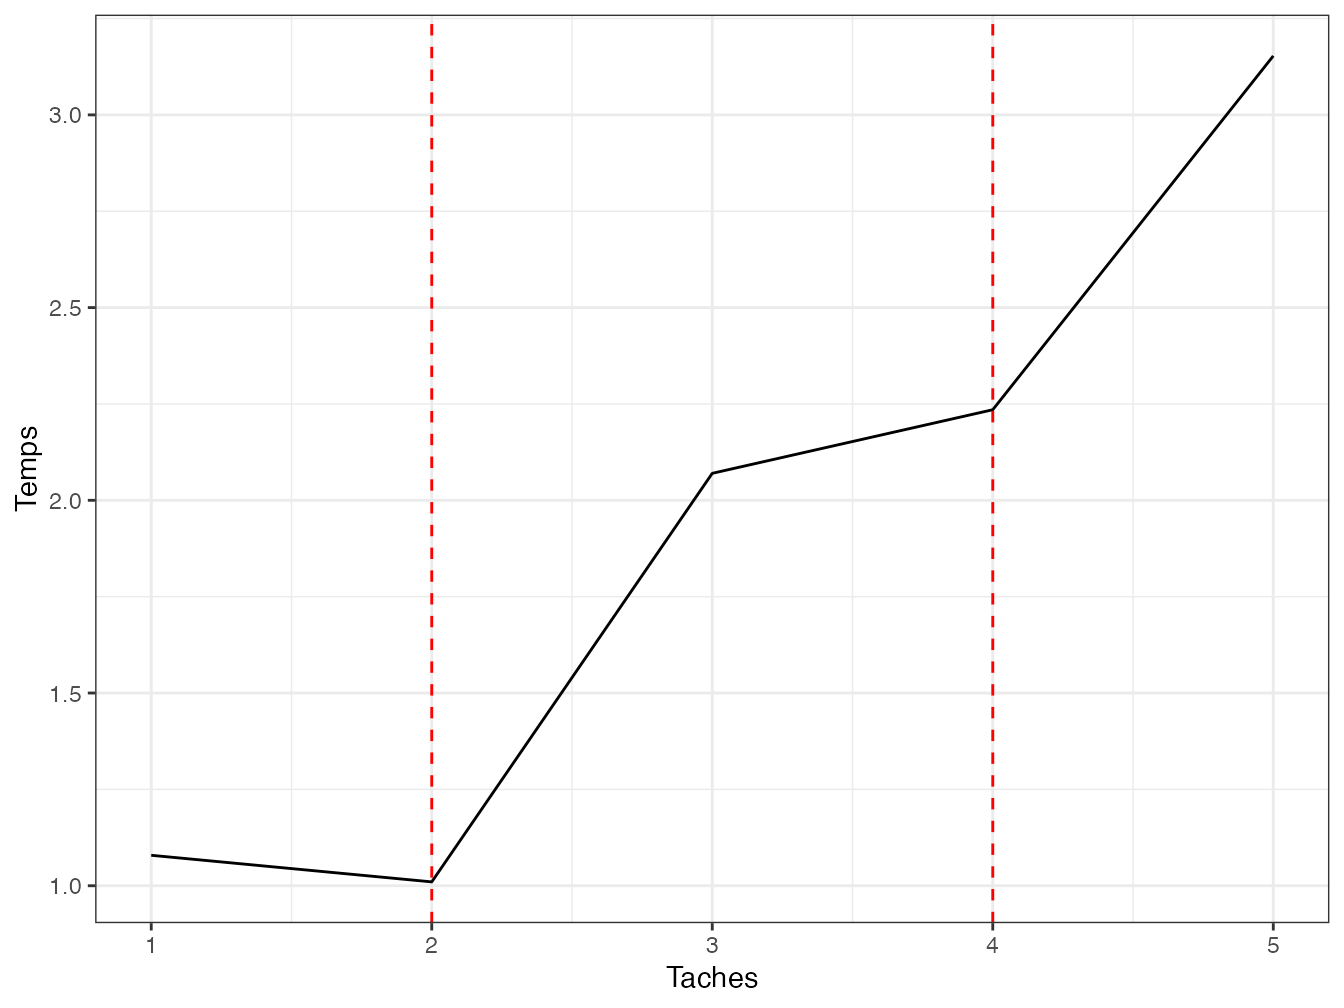
\includegraphics[width=0.8\linewidth]{travailleR_files/figure-latex/r-parallele-1} 

}

\caption[Temps d'exécution en parallèle]{Temps d'exécution en parallèle de tâches nécessitant une seconde (chaque tâche est une pause d'une seconde). Le nombre de tâches varie de 1 à deux fois le nombre de cœurs utilisés (égal à \texttt{2}) plus une.}\label{fig:r-parallele}
\end{figure}

\normalsize

La forme théorique de cette courbe est la suivante:

\begin{itemize}
\tightlist
\item
  pour une tâche, le temps est égal à une seconde plus le temps de mise en place de la parallélisation;
\item
  le temps devrait rester stable jusqu'au nombre de cœurs utilisés;
\item
  quand les cœurs sont tous utilisés (pointillés rouges), le temps devrait augmenter d'une seconde puis rester stable jusqu'à la limite suivante.
\end{itemize}

En pratique, le temps de calcul est déterminé par d'autres facteurs difficilement prévisibles.
La bonne pratique est d'adapter le nombre de tâches au nombre de cœurs sous peine de perte de performance.

\subsection{parLapply (socket)}\label{parlapply-socket}

\texttt{parLapply} nécessite de créer un cluster, exporter les variables utiles sur chaque noeud, charger les packages nécessaires sur chaque noeud, exécuter le code et enfin arrêter le cluster.
Le code de chaque étape se trouve dans la fonction \texttt{mclapply.hack} ci-dessus.

Pour un usage courant, \texttt{mclapply} est plus rapide, sauf sous Windows, et plus simple (y compris sous Windows grâce au contournement ci-dessus.)

\subsection{foreach}\label{foreach}

\subsubsection{Fonctionnement}\label{fonctionnement}

Le package \textbf{foreach} permet un usage avancé de la parallélisation.
Lire ses vignettes.

\scriptsize

\begin{Shaded}
\begin{Highlighting}[]
\CommentTok{\# Manuel}
\FunctionTok{vignette}\NormalTok{(}\StringTok{"foreach"}\NormalTok{, }\StringTok{"foreach"}\NormalTok{)}
\CommentTok{\# Boucles imbriquées}
\FunctionTok{vignette}\NormalTok{(}\StringTok{"nested"}\NormalTok{, }\StringTok{"foreach"}\NormalTok{)}
\end{Highlighting}
\end{Shaded}

\normalsize

Indépendamment de la parallélisation, \textbf{foreach} redéfinit les boucles \emph{for}.

\scriptsize

\begin{Shaded}
\begin{Highlighting}[]
\ControlFlowTok{for}\NormalTok{ (i }\ControlFlowTok{in} \DecValTok{1}\SpecialCharTok{:}\DecValTok{3}\NormalTok{) \{}
  \FunctionTok{f}\NormalTok{(i)}
\NormalTok{\}}
\CommentTok{\# devient}
\FunctionTok{library}\NormalTok{(}\StringTok{"foreach"}\NormalTok{)}
\FunctionTok{foreach}\NormalTok{(}\AttributeTok{i =} \DecValTok{1}\SpecialCharTok{:}\DecValTok{3}\NormalTok{) }\SpecialCharTok{\%do\%}\NormalTok{ \{}
  \FunctionTok{f}\NormalTok{(i)}
\NormalTok{\}}
\end{Highlighting}
\end{Shaded}

\begin{verbatim}
## [[1]]
## [1] 1
## 
## [[2]]
## [1] 2
## 
## [[3]]
## [1] 3
\end{verbatim}

\normalsize

La fonction \texttt{foreach} retourne une liste contenant les résultats de chaque boucle.
Les éléments de la liste peuvent être combinés par une fonction quelconque, comme \texttt{c}.

\scriptsize

\begin{Shaded}
\begin{Highlighting}[]
\FunctionTok{foreach}\NormalTok{(}\AttributeTok{i =} \DecValTok{1}\SpecialCharTok{:}\DecValTok{3}\NormalTok{, }\AttributeTok{.combine =} \StringTok{"c"}\NormalTok{) }\SpecialCharTok{\%do\%}\NormalTok{ \{}
  \FunctionTok{f}\NormalTok{(i)}
\NormalTok{\}}
\end{Highlighting}
\end{Shaded}

\begin{verbatim}
## [1] 1 2 3
\end{verbatim}

\normalsize

La fonction \texttt{foreach} est capable d'utiliser des itérateurs, c'est-à-dire des fonctions qui ne passent à la boucle que les données dont elle a besoin sans charger les autres en mémoire.
Ici, l'itérateur \texttt{icount} passe les valeurs 1, 2 et 3 individuellement, sans charger le vecteur 1:3 en mémoire.

\scriptsize

\begin{Shaded}
\begin{Highlighting}[]
\FunctionTok{library}\NormalTok{(}\StringTok{"iterators"}\NormalTok{)}
\FunctionTok{foreach}\NormalTok{(}\AttributeTok{i =} \FunctionTok{icount}\NormalTok{(}\DecValTok{3}\NormalTok{), }\AttributeTok{.combine =} \StringTok{"c"}\NormalTok{) }\SpecialCharTok{\%do\%}\NormalTok{ \{}
  \FunctionTok{f}\NormalTok{(i)}
\NormalTok{\}}
\end{Highlighting}
\end{Shaded}

\begin{verbatim}
## [1] 1 2 3
\end{verbatim}

\normalsize

Elle est donc très utile quand chaque objet de la boucle utilise une grande quantité de mémoire.

\subsubsection{Parallélisation}\label{paralluxe9lisation}

Remplacer l'opérateur \texttt{\%do\%} par \texttt{\%dopar\%} parallélise les boucles, à condition qu'un adaptateur, c'est-à-dire un package intermédiaire entre \texttt{foreach} et un package chargé de l'implémentation de la parallélisation, soit chargé.
\textbf{doParallel} est un adaptateur pour utiliser le package \textbf{parallel} livré avec R.

\scriptsize

\begin{Shaded}
\begin{Highlighting}[]
\FunctionTok{library}\NormalTok{(doParallel)}
\FunctionTok{registerDoParallel}\NormalTok{(}\AttributeTok{cores =}\NormalTok{ nbCoeurs)}
\CommentTok{\# Série}
\FunctionTok{system.time}\NormalTok{(}
  \FunctionTok{foreach}\NormalTok{(}\AttributeTok{i =} \FunctionTok{icount}\NormalTok{(nbCoeurs), }\AttributeTok{.combine =} \StringTok{"c"}\NormalTok{) }\SpecialCharTok{\%do\%}\NormalTok{ \{}\FunctionTok{f}\NormalTok{(i)\}}
\NormalTok{)}
\end{Highlighting}
\end{Shaded}

\begin{verbatim}
##    user  system elapsed 
##   0.002   0.000   0.736
\end{verbatim}

\begin{Shaded}
\begin{Highlighting}[]
\CommentTok{\# Parallèle}
\FunctionTok{system.time}\NormalTok{(}
  \FunctionTok{foreach}\NormalTok{(}\AttributeTok{i =} \FunctionTok{icount}\NormalTok{(nbCoeurs), }\AttributeTok{.combine =} \StringTok{"c"}\NormalTok{) }\SpecialCharTok{\%dopar\%}\NormalTok{ \{}\FunctionTok{f}\NormalTok{(i)\}}
\NormalTok{)}
\end{Highlighting}
\end{Shaded}

\begin{verbatim}
##    user  system elapsed 
##   0.004   0.014   0.319
\end{verbatim}

\normalsize

Le coût fixe de la parallélisation est faible.

\subsection{future}\label{future}

Le package \textbf{future} permet d'abstraire le code de l'implémentation de la parallélisation.
Il est au centre d'un écosystème de packages facilitent son utilisation\footnote{\url{https://www.futureverse.org/}}.

La stratégie de parallélisation utilisée est déclarée par la fonction \texttt{plan()}.
Le stratégie par défaut est \texttt{sequential}, monotâche.
Les stratégies \texttt{multicore} et \texttt{multisession} reposent respectivement sur les techniques \emph{fork} et \emph{socket} vues plus haut.
D'autres stratégies sont disponibles pour utiliser des clusters physiques (plusieurs ordinateurs préparés pour exécuter R ensemble): la documentation de \textbf{future} détaille comment le faire.

Nous utiliserons ici la stratégie \texttt{multisession} qui fonctionne sur l'ordinateur local, quel que soit sont système d'exploitation.

\scriptsize

\begin{Shaded}
\begin{Highlighting}[]
\FunctionTok{library}\NormalTok{(}\StringTok{"future"}\NormalTok{)}
\CommentTok{\# Stratégie socket sur tous les coeurs disponibles sauf 1}
\NormalTok{usedCores }\OtherTok{\textless{}{-}} \FunctionTok{availableCores}\NormalTok{(}\AttributeTok{omit =} \DecValTok{1}\NormalTok{)}
\FunctionTok{plan}\NormalTok{(multisession, }\AttributeTok{workers =}\NormalTok{ usedCores)}
\end{Highlighting}
\end{Shaded}

\normalsize

Le package \textbf{future.apply} permet de paralléliser sans effort toutes les boucles \texttt{*apply()} et \texttt{replicate()} en préfixant leur nom par \texttt{future\_}.

\scriptsize

\begin{Shaded}
\begin{Highlighting}[]
\FunctionTok{library}\NormalTok{(}\StringTok{"future.apply"}\NormalTok{)}
\FunctionTok{system.time}\NormalTok{(}\FunctionTok{future\_replicate}\NormalTok{(usedCores }\SpecialCharTok{{-}} \DecValTok{1}\NormalTok{, }\FunctionTok{f}\NormalTok{(usedCores)))}
\end{Highlighting}
\end{Shaded}

\begin{verbatim}
##    user  system elapsed 
##   0.023   0.000   0.454
\end{verbatim}

\normalsize

Les boucles foreach peuvent être parallélisées avec le package \textbf{doFuture} en remplaçant simplement \texttt{\%dopar\%} par \texttt{\%dofuture\%}.

\scriptsize

\begin{Shaded}
\begin{Highlighting}[]
\FunctionTok{library}\NormalTok{(}\StringTok{"doFuture"}\NormalTok{)}
\FunctionTok{system.time}\NormalTok{(}
  \FunctionTok{foreach}\NormalTok{(}\AttributeTok{i =} \FunctionTok{icount}\NormalTok{(nbCoeurs), }\AttributeTok{.combine =} \StringTok{"c"}\NormalTok{) }\SpecialCharTok{\%dofuture\%}\NormalTok{ \{}\FunctionTok{f}\NormalTok{(i)\}}
\NormalTok{)}
\end{Highlighting}
\end{Shaded}

\begin{verbatim}
##    user  system elapsed 
##   0.038   0.001   0.492
\end{verbatim}

\normalsize

La stratégie est rétablie à \texttt{sequential} à la fin.

\scriptsize

\begin{Shaded}
\begin{Highlighting}[]
\FunctionTok{plan}\NormalTok{(sequential)}
\end{Highlighting}
\end{Shaded}

\normalsize

\section{Etude de cas}\label{sec:cas}

Cette étude de cas permet de tester les différentes techniques vues plus haut pour résoudre un problème concret.
L'objectif est de calculer la distance moyenne entre deux points d'un semis aléatoire de 1000 points dans une fenêtre carrée de côté 1.

Son espérance est calculable\footnote{\url{https://mindyourdecisions.com/blog/2016/07/03/distance-between-two-random-points-in-a-square-sunday-puzzle/}}.
Elle est égale à \(\frac{2+\sqrt{2}+5\ln{(1+\sqrt{2})}}{15} \approx 0,5214\).

\subsection{Création des données}\label{cruxe9ation-des-donnuxe9es}

Le semis de points est créé avec le package \textbf{spatstat}.

\scriptsize

\begin{Shaded}
\begin{Highlighting}[]
\NormalTok{NbPoints }\OtherTok{\textless{}{-}} \DecValTok{1000}
\FunctionTok{library}\NormalTok{(}\StringTok{"spatstat"}\NormalTok{)}
\NormalTok{X }\OtherTok{\textless{}{-}} \FunctionTok{runifpoint}\NormalTok{(NbPoints)}
\end{Highlighting}
\end{Shaded}

\normalsize

\subsection{Spatstat}\label{spatstat}

La fonction \texttt{pairdist()} de \textbf{spatstat} retourne la matrice des distances entre les points.
La distance moyenne est calculée en divisant la somme par le nombre de paires de points distincts.

\scriptsize

\begin{Shaded}
\begin{Highlighting}[]
\NormalTok{mb }\OtherTok{\textless{}{-}} \FunctionTok{microbenchmark}\NormalTok{(d }\OtherTok{\textless{}{-}} \FunctionTok{sum}\NormalTok{(}\FunctionTok{pairdist}\NormalTok{(X)) }\SpecialCharTok{/}\NormalTok{ NbPoints }\SpecialCharTok{/}\NormalTok{ (NbPoints }\SpecialCharTok{{-}} \DecValTok{1}\NormalTok{))}
\FunctionTok{autoplot}\NormalTok{(mb)}
\end{Highlighting}
\end{Shaded}

\begin{center}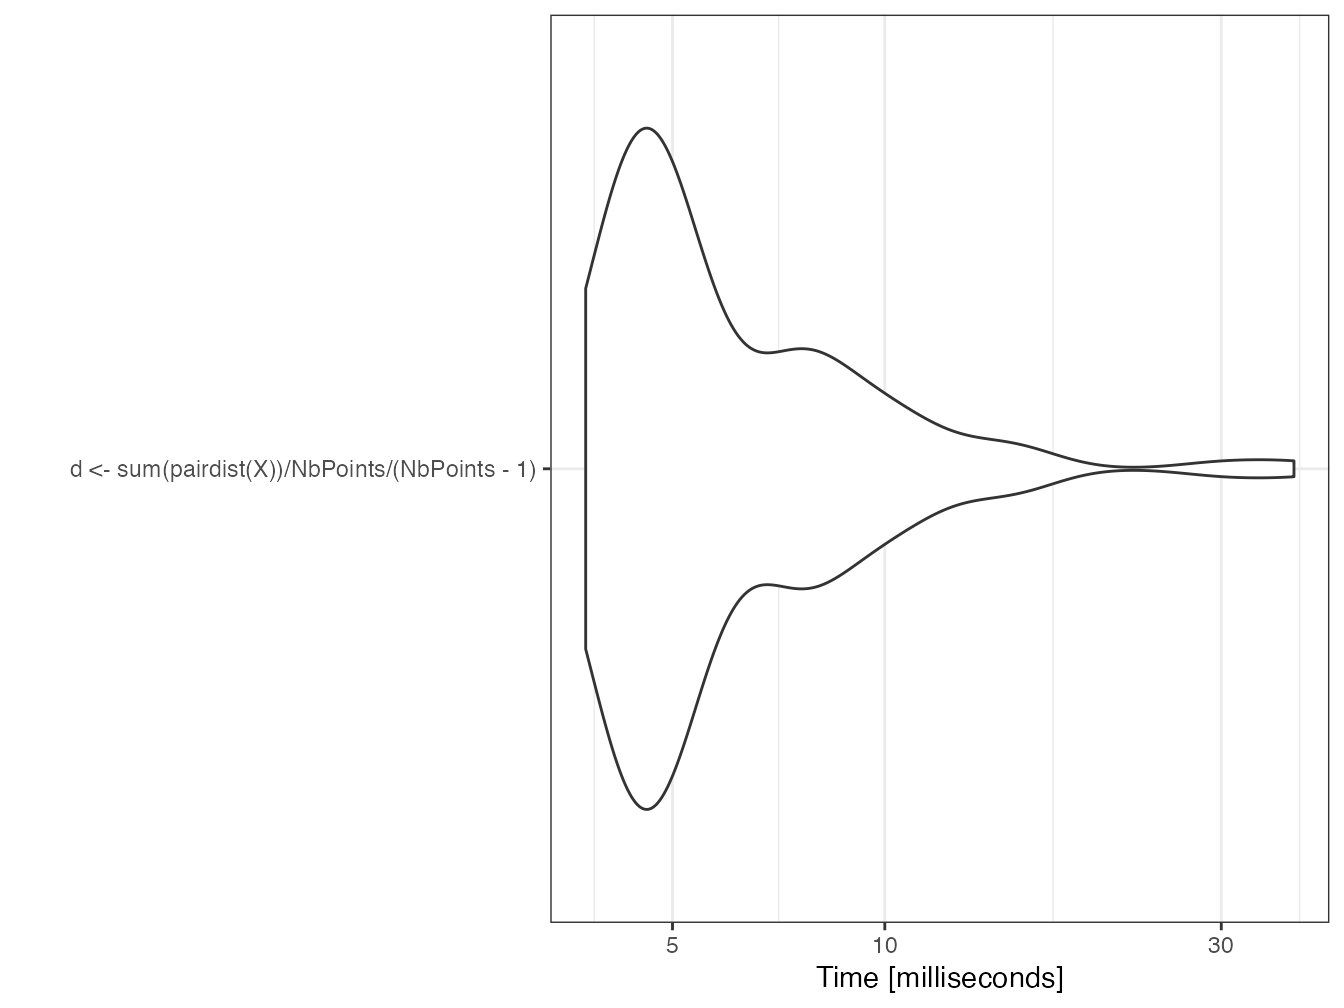
\includegraphics[width=0.8\linewidth]{travailleR_files/figure-latex/pairdist-1} \end{center}

\begin{Shaded}
\begin{Highlighting}[]
\NormalTok{d}
\end{Highlighting}
\end{Shaded}

\begin{verbatim}
## [1] 0.5154879
\end{verbatim}

\normalsize

La fonction est rapide parce qu'elle est codée en langage C dans le package \textbf{spatstat} pour le cœur de ses calculs.

\subsection{apply}\label{apply}

La distance peut être calculée par deux \texttt{sapply()} imbriqués.

\scriptsize

\begin{Shaded}
\begin{Highlighting}[]
\NormalTok{fsapply1 }\OtherTok{\textless{}{-}} \ControlFlowTok{function}\NormalTok{() \{}
\NormalTok{  distances }\OtherTok{\textless{}{-}} \FunctionTok{sapply}\NormalTok{(}
    \DecValTok{1}\SpecialCharTok{:}\NormalTok{NbPoints, }
    \AttributeTok{FUN =} \ControlFlowTok{function}\NormalTok{(i) \{}
      \FunctionTok{sapply}\NormalTok{(}
        \DecValTok{1}\SpecialCharTok{:}\NormalTok{NbPoints, }
        \AttributeTok{FUN =} \ControlFlowTok{function}\NormalTok{(j) \{}
          \FunctionTok{sqrt}\NormalTok{((X}\SpecialCharTok{$}\NormalTok{x[i] }\SpecialCharTok{{-}}\NormalTok{ X}\SpecialCharTok{$}\NormalTok{x[j])}\SpecialCharTok{\^{}}\DecValTok{2} \SpecialCharTok{+}\NormalTok{ (X}\SpecialCharTok{$}\NormalTok{y[i] }\SpecialCharTok{{-}}\NormalTok{ X}\SpecialCharTok{$}\NormalTok{y[j])}\SpecialCharTok{\^{}}\DecValTok{2}\NormalTok{)}
\NormalTok{        \}}
\NormalTok{      )}
\NormalTok{    \}}
\NormalTok{  )}
  \FunctionTok{return}\NormalTok{(}\FunctionTok{sum}\NormalTok{(distances) }\SpecialCharTok{/}\NormalTok{ NbPoints }\SpecialCharTok{/}\NormalTok{ (NbPoints }\SpecialCharTok{{-}} \DecValTok{1}\NormalTok{))}
\NormalTok{\}}
\FunctionTok{system.time}\NormalTok{(d }\OtherTok{\textless{}{-}} \FunctionTok{fsapply1}\NormalTok{())}
\end{Highlighting}
\end{Shaded}

\begin{verbatim}
##    user  system elapsed 
##   2.215   0.007   2.222
\end{verbatim}

\begin{Shaded}
\begin{Highlighting}[]
\NormalTok{d}
\end{Highlighting}
\end{Shaded}

\begin{verbatim}
## [1] 0.5154879
\end{verbatim}

\normalsize

Un peu de temps peut être gagnée en remplaçant \texttt{sapply} par \texttt{vapply}: le format des résultats n'a pas à être déterminé par la fonction.
Le gain est négligeable sur un long calcul comme celui-ci mais important pour des calculs courts.

\scriptsize

\begin{Shaded}
\begin{Highlighting}[]
\NormalTok{fsapply2 }\OtherTok{\textless{}{-}} \ControlFlowTok{function}\NormalTok{() \{}
\NormalTok{  distances }\OtherTok{\textless{}{-}} \FunctionTok{vapply}\NormalTok{(}
    \DecValTok{1}\SpecialCharTok{:}\NormalTok{NbPoints, }
    \AttributeTok{FUN =} \ControlFlowTok{function}\NormalTok{(i) \{}
      \FunctionTok{vapply}\NormalTok{(}
        \DecValTok{1}\SpecialCharTok{:}\NormalTok{NbPoints, }
        \AttributeTok{FUN =} \ControlFlowTok{function}\NormalTok{(j) \{}
          \FunctionTok{sqrt}\NormalTok{((X}\SpecialCharTok{$}\NormalTok{x[i] }\SpecialCharTok{{-}}\NormalTok{ X}\SpecialCharTok{$}\NormalTok{x[j])}\SpecialCharTok{\^{}}\DecValTok{2} \SpecialCharTok{+}\NormalTok{ (X}\SpecialCharTok{$}\NormalTok{y[i] }\SpecialCharTok{{-}}\NormalTok{ X}\SpecialCharTok{$}\NormalTok{y[j])}\SpecialCharTok{\^{}}\DecValTok{2}\NormalTok{)}
\NormalTok{        \}, }
        \AttributeTok{FUN.VALUE =} \DecValTok{0}
\NormalTok{      )}
\NormalTok{    \}, }
    \AttributeTok{FUN.VALUE =} \DecValTok{1}\SpecialCharTok{:}\DecValTok{1000} \SpecialCharTok{+} \DecValTok{0}
\NormalTok{  )}
  \FunctionTok{return}\NormalTok{(}\FunctionTok{sum}\NormalTok{(distances) }\SpecialCharTok{/}\NormalTok{ NbPoints }\SpecialCharTok{/}\NormalTok{ (NbPoints }\SpecialCharTok{{-}} \DecValTok{1}\NormalTok{))}
\NormalTok{\}}
\FunctionTok{system.time}\NormalTok{(d }\OtherTok{\textless{}{-}} \FunctionTok{fsapply2}\NormalTok{())}
\end{Highlighting}
\end{Shaded}

\begin{verbatim}
##    user  system elapsed 
##   2.258   0.006   2.263
\end{verbatim}

\begin{Shaded}
\begin{Highlighting}[]
\NormalTok{d}
\end{Highlighting}
\end{Shaded}

\begin{verbatim}
## [1] 0.5154879
\end{verbatim}

\normalsize
Le format de sortie n'est pas toujours évident à écrire:

\begin{itemize}
\tightlist
\item
  il doit respecter la taille des données: un vecteur de taille 1000 pour la boucle externe, un scalaire pour la boucle interne.
\item
  il doit respecter leur type: \texttt{0} pour un entier, \texttt{0.0} pour un réel. Dans la boucle externe, l'ajout de \texttt{0.0} au vecteur d'entiers le transforme en vecteur de réels.
\end{itemize}

Une amélioration plus significative consiste à ne calculer les racines carrées qu'à la fin de la boucle, pour profiter de la vectorisation de la fonction.

\scriptsize

\begin{Shaded}
\begin{Highlighting}[]
\NormalTok{fsapply3 }\OtherTok{\textless{}{-}} \ControlFlowTok{function}\NormalTok{() \{}
\NormalTok{  distances }\OtherTok{\textless{}{-}} \FunctionTok{vapply}\NormalTok{(}
    \DecValTok{1}\SpecialCharTok{:}\NormalTok{NbPoints, }
    \AttributeTok{FUN =} \ControlFlowTok{function}\NormalTok{(i) \{}
      \FunctionTok{vapply}\NormalTok{(}
        \DecValTok{1}\SpecialCharTok{:}\NormalTok{NbPoints, }
        \AttributeTok{FUN =} \ControlFlowTok{function}\NormalTok{(j) \{}
\NormalTok{          (X}\SpecialCharTok{$}\NormalTok{x[i] }\SpecialCharTok{{-}}\NormalTok{ X}\SpecialCharTok{$}\NormalTok{x[j])}\SpecialCharTok{\^{}}\DecValTok{2} \SpecialCharTok{+}\NormalTok{ (X}\SpecialCharTok{$}\NormalTok{y[i] }\SpecialCharTok{{-}}\NormalTok{ X}\SpecialCharTok{$}\NormalTok{y[j])}\SpecialCharTok{\^{}}\DecValTok{2}
\NormalTok{        \}, }
        \AttributeTok{FUN.VALUE =} \DecValTok{0}
\NormalTok{      )}
\NormalTok{    \}, }
    \AttributeTok{FUN.VALUE =} \DecValTok{1}\SpecialCharTok{:}\DecValTok{1000} \SpecialCharTok{+} \DecValTok{0}
\NormalTok{  )}
  \FunctionTok{return}\NormalTok{(}\FunctionTok{sum}\NormalTok{(}\FunctionTok{sqrt}\NormalTok{(distances)) }\SpecialCharTok{/}\NormalTok{ NbPoints }\SpecialCharTok{/}\NormalTok{ (NbPoints }\SpecialCharTok{{-}} \DecValTok{1}\NormalTok{))}
\NormalTok{\}}
\FunctionTok{system.time}\NormalTok{(d }\OtherTok{\textless{}{-}} \FunctionTok{fsapply3}\NormalTok{())}
\end{Highlighting}
\end{Shaded}

\begin{verbatim}
##    user  system elapsed 
##   2.155   0.004   2.160
\end{verbatim}

\begin{Shaded}
\begin{Highlighting}[]
\NormalTok{d}
\end{Highlighting}
\end{Shaded}

\begin{verbatim}
## [1] 0.5154879
\end{verbatim}

\normalsize

Les calculs sont effectués deux fois (distance entre les points \(i\) et \(j\), mais aussi entre les points \(j\) et \(i\)): un test sur les indices permet de diviser presque le temps par 2 (pas tout à fait parce que les boucles sans calcul, qui retournent \(0\), prennent du temps).

\scriptsize

\begin{Shaded}
\begin{Highlighting}[]
\NormalTok{fsapply4 }\OtherTok{\textless{}{-}} \ControlFlowTok{function}\NormalTok{() \{}
\NormalTok{  distances }\OtherTok{\textless{}{-}} \FunctionTok{vapply}\NormalTok{(}
    \DecValTok{1}\SpecialCharTok{:}\NormalTok{NbPoints, }
    \AttributeTok{FUN =} \ControlFlowTok{function}\NormalTok{(i) \{}
      \FunctionTok{vapply}\NormalTok{(}
        \DecValTok{1}\SpecialCharTok{:}\NormalTok{NbPoints, }
        \AttributeTok{FUN =} \ControlFlowTok{function}\NormalTok{(j) \{}
          \ControlFlowTok{if}\NormalTok{ (j }\SpecialCharTok{\textgreater{}}\NormalTok{ i) \{}
\NormalTok{            (X}\SpecialCharTok{$}\NormalTok{x[i] }\SpecialCharTok{{-}}\NormalTok{ X}\SpecialCharTok{$}\NormalTok{x[j])}\SpecialCharTok{\^{}}\DecValTok{2} \SpecialCharTok{+}\NormalTok{ (X}\SpecialCharTok{$}\NormalTok{y[i] }\SpecialCharTok{{-}}\NormalTok{ X}\SpecialCharTok{$}\NormalTok{y[j])}\SpecialCharTok{\^{}}\DecValTok{2}
\NormalTok{          \} }\ControlFlowTok{else}\NormalTok{ \{}
            \DecValTok{0}
\NormalTok{          \}}
\NormalTok{        \}, }
        \AttributeTok{FUN.VALUE =} \FloatTok{0.0}
\NormalTok{      )}
\NormalTok{    \}, }
    \AttributeTok{FUN.VALUE =} \DecValTok{1}\SpecialCharTok{:}\DecValTok{1000} \SpecialCharTok{+} \DecValTok{0}
\NormalTok{  )}
  \FunctionTok{return}\NormalTok{(}\FunctionTok{sum}\NormalTok{(}\FunctionTok{sqrt}\NormalTok{(distances)) }\SpecialCharTok{/}\NormalTok{ NbPoints }\SpecialCharTok{/}\NormalTok{ (NbPoints }\SpecialCharTok{{-}} \DecValTok{1}\NormalTok{) }\SpecialCharTok{*} \DecValTok{2}\NormalTok{)}
\NormalTok{\}}
\FunctionTok{system.time}\NormalTok{(d }\OtherTok{\textless{}{-}} \FunctionTok{fsapply4}\NormalTok{())}
\end{Highlighting}
\end{Shaded}

\begin{verbatim}
##    user  system elapsed 
##   1.256   0.002   1.258
\end{verbatim}

\begin{Shaded}
\begin{Highlighting}[]
\NormalTok{d}
\end{Highlighting}
\end{Shaded}

\begin{verbatim}
## [1] 0.5154879
\end{verbatim}

\normalsize

En parallèle, le temps de calcul n'est pas amélioré sous Windows parce que les tâches individuelles sont trop courtes.
Sous MacOS ou Linux, le calcul est accéléré.

\scriptsize

\begin{Shaded}
\begin{Highlighting}[]
\NormalTok{fsapply5 }\OtherTok{\textless{}{-}} \ControlFlowTok{function}\NormalTok{() \{}
\NormalTok{  distances }\OtherTok{\textless{}{-}} \FunctionTok{mclapply}\NormalTok{(}
    \DecValTok{1}\SpecialCharTok{:}\NormalTok{NbPoints, }
    \CommentTok{\# Avoid naming the argument because it is named FUN in mclapply()}
    \CommentTok{\# but fun in parLapply() used by  mclapply.hack()}
    \ControlFlowTok{function}\NormalTok{(i) \{}
      \FunctionTok{vapply}\NormalTok{(}
        \DecValTok{1}\SpecialCharTok{:}\NormalTok{NbPoints, }
        \AttributeTok{FUN =} \ControlFlowTok{function}\NormalTok{(j) \{}
          \ControlFlowTok{if}\NormalTok{ (j }\SpecialCharTok{\textgreater{}}\NormalTok{ i) \{}
\NormalTok{            (X}\SpecialCharTok{$}\NormalTok{x[i] }\SpecialCharTok{{-}}\NormalTok{ X}\SpecialCharTok{$}\NormalTok{x[j])}\SpecialCharTok{\^{}}\DecValTok{2} \SpecialCharTok{+}\NormalTok{ (X}\SpecialCharTok{$}\NormalTok{y[i] }\SpecialCharTok{{-}}\NormalTok{ X}\SpecialCharTok{$}\NormalTok{y[j])}\SpecialCharTok{\^{}}\DecValTok{2}
\NormalTok{          \} }\ControlFlowTok{else}\NormalTok{ \{}
            \DecValTok{0}
\NormalTok{          \}}
\NormalTok{        \}, }
        \DecValTok{0}
\NormalTok{      )}
\NormalTok{    \}}
\NormalTok{  )}
  \FunctionTok{return}\NormalTok{(}
    \FunctionTok{sum}\NormalTok{(}\FunctionTok{sqrt}\NormalTok{(}\FunctionTok{simplify2array}\NormalTok{(distances))) }\SpecialCharTok{/}\NormalTok{ NbPoints }\SpecialCharTok{/}\NormalTok{ (NbPoints }\SpecialCharTok{{-}} \DecValTok{1}\NormalTok{) }\SpecialCharTok{*} \DecValTok{2}
\NormalTok{  )}
\NormalTok{\}}
\FunctionTok{system.time}\NormalTok{(d }\OtherTok{\textless{}{-}} \FunctionTok{fsapply5}\NormalTok{())}
\end{Highlighting}
\end{Shaded}

\begin{verbatim}
##    user  system elapsed 
##   1.371   0.208   1.021
\end{verbatim}

\begin{Shaded}
\begin{Highlighting}[]
\NormalTok{d}
\end{Highlighting}
\end{Shaded}

\begin{verbatim}
## [1] 0.5154879
\end{verbatim}

\normalsize

\subsection{future.apply}\label{future.apply}

La fonction \texttt{fsapply4()} optimisée plus haut peut être parallélisée directement en préfixant la fonction \texttt{vapply} par \texttt{future\_}.
Seule la boucle principale est parallélisée: l'imbrication de \texttt{future\_vapply()} ferait s'écrouler la performance.

\scriptsize

\begin{Shaded}
\begin{Highlighting}[]
\FunctionTok{library}\NormalTok{(}\StringTok{"future.apply"}\NormalTok{)}
\CommentTok{\# Stratégie socket sur tous les coeurs disponibles sauf 1}
\FunctionTok{plan}\NormalTok{(multisession, }\AttributeTok{workers =} \FunctionTok{availableCores}\NormalTok{(}\AttributeTok{omit =} \DecValTok{1}\NormalTok{))}
\NormalTok{future\_fsapply4\_ }\OtherTok{\textless{}{-}} \ControlFlowTok{function}\NormalTok{() \{}
\NormalTok{  distances }\OtherTok{\textless{}{-}} \FunctionTok{future\_vapply}\NormalTok{(}\DecValTok{1}\SpecialCharTok{:}\NormalTok{NbPoints, }\ControlFlowTok{function}\NormalTok{(i) \{}
    \FunctionTok{vapply}\NormalTok{(}\DecValTok{1}\SpecialCharTok{:}\NormalTok{NbPoints, }\ControlFlowTok{function}\NormalTok{(j) \{}
      \ControlFlowTok{if}\NormalTok{ (j }\SpecialCharTok{\textgreater{}}\NormalTok{ i) \{}
\NormalTok{        (X}\SpecialCharTok{$}\NormalTok{x[i] }\SpecialCharTok{{-}}\NormalTok{ X}\SpecialCharTok{$}\NormalTok{x[j])}\SpecialCharTok{\^{}}\DecValTok{2} \SpecialCharTok{+}\NormalTok{ (X}\SpecialCharTok{$}\NormalTok{y[i] }\SpecialCharTok{{-}}\NormalTok{ X}\SpecialCharTok{$}\NormalTok{y[j])}\SpecialCharTok{\^{}}\DecValTok{2}
\NormalTok{      \} }\ControlFlowTok{else}\NormalTok{ \{}
        \DecValTok{0}
\NormalTok{      \}}
\NormalTok{    \}, }\DecValTok{0}\NormalTok{)}
\NormalTok{  \}, }\DecValTok{1}\SpecialCharTok{:}\DecValTok{1000} \SpecialCharTok{+} \DecValTok{0}\NormalTok{)}
  \FunctionTok{return}\NormalTok{(}\FunctionTok{sum}\NormalTok{(}\FunctionTok{sqrt}\NormalTok{(distances)) }\SpecialCharTok{/}\NormalTok{ NbPoints }\SpecialCharTok{/}\NormalTok{ (NbPoints }\SpecialCharTok{{-}} \DecValTok{1}\NormalTok{) }\SpecialCharTok{*} \DecValTok{2}\NormalTok{)}
\NormalTok{\}}
\FunctionTok{system.time}\NormalTok{(d }\OtherTok{\textless{}{-}} \FunctionTok{future\_fsapply4\_}\NormalTok{())}
\end{Highlighting}
\end{Shaded}

\begin{verbatim}
##    user  system elapsed 
##   0.048   0.007   1.025
\end{verbatim}

\begin{Shaded}
\begin{Highlighting}[]
\NormalTok{d}
\end{Highlighting}
\end{Shaded}

\begin{verbatim}
## [1] 0.5154879
\end{verbatim}

\begin{Shaded}
\begin{Highlighting}[]
\FunctionTok{plan}\NormalTok{(sequential)}
\end{Highlighting}
\end{Shaded}

\normalsize

\subsection{boucle for}\label{boucle-for}

Une boucle for est plus rapide et consomme moins de mémoire parce qu'elle ne stocke pas la matrice de distances.

\scriptsize

\begin{Shaded}
\begin{Highlighting}[]
\NormalTok{distance }\OtherTok{\textless{}{-}} \DecValTok{0}
\NormalTok{ffor }\OtherTok{\textless{}{-}} \ControlFlowTok{function}\NormalTok{() \{}
  \ControlFlowTok{for}\NormalTok{ (i }\ControlFlowTok{in} \DecValTok{1}\SpecialCharTok{:}\NormalTok{(NbPoints }\SpecialCharTok{{-}} \DecValTok{1}\NormalTok{)) \{}
    \ControlFlowTok{for}\NormalTok{ (j }\ControlFlowTok{in}\NormalTok{ (i }\SpecialCharTok{+} \DecValTok{1}\NormalTok{)}\SpecialCharTok{:}\NormalTok{NbPoints) \{}
\NormalTok{        distance }\OtherTok{\textless{}{-}}\NormalTok{ distance }\SpecialCharTok{+} \FunctionTok{sqrt}\NormalTok{((X}\SpecialCharTok{$}\NormalTok{x[i] }\SpecialCharTok{{-}}\NormalTok{ X}\SpecialCharTok{$}\NormalTok{x[j])}\SpecialCharTok{\^{}}\DecValTok{2} \SpecialCharTok{+}\NormalTok{ (X}\SpecialCharTok{$}\NormalTok{y[i] }\SpecialCharTok{{-}}\NormalTok{ X}\SpecialCharTok{$}\NormalTok{y[j])}\SpecialCharTok{\^{}}\DecValTok{2}\NormalTok{)}
\NormalTok{    \}}
\NormalTok{  \}}
  \FunctionTok{return}\NormalTok{(distance }\SpecialCharTok{/}\NormalTok{ NbPoints }\SpecialCharTok{/}\NormalTok{ (NbPoints }\SpecialCharTok{{-}} \DecValTok{1}\NormalTok{) }\SpecialCharTok{*} \DecValTok{2}\NormalTok{)}
\NormalTok{\}}
\CommentTok{\# Temps de calcul, mémorisé}
\NormalTok{(for\_time }\OtherTok{\textless{}{-}} \FunctionTok{system.time}\NormalTok{(d }\OtherTok{\textless{}{-}} \FunctionTok{ffor}\NormalTok{()))}
\end{Highlighting}
\end{Shaded}

\begin{verbatim}
##    user  system elapsed 
##   0.811   0.002   0.813
\end{verbatim}

\begin{Shaded}
\begin{Highlighting}[]
\NormalTok{d}
\end{Highlighting}
\end{Shaded}

\begin{verbatim}
## [1] 0.5154879
\end{verbatim}

\normalsize

C'est la façon la plus simple et efficace d'écrire ce code sans parallélisation et en se limitant au langage de R.

\subsection{boucle foreach}\label{boucle-foreach}

La parallélisation exécute des boucles \texttt{for} à l'intérieur d'une boucle foreach, ce qui est assez efficace.
En revanche, les distances sont calculées deux fois.

\scriptsize

\begin{Shaded}
\begin{Highlighting}[]
\FunctionTok{registerDoParallel}\NormalTok{(}\AttributeTok{cores =} \FunctionTok{detectCores}\NormalTok{())}
\NormalTok{fforeach3 }\OtherTok{\textless{}{-}} \ControlFlowTok{function}\NormalTok{(Y) \{}
\NormalTok{  distances }\OtherTok{\textless{}{-}} \FunctionTok{foreach}\NormalTok{(}\AttributeTok{i =} \FunctionTok{icount}\NormalTok{(Y}\SpecialCharTok{$}\NormalTok{n), }\AttributeTok{.combine =} \StringTok{\textquotesingle{}+\textquotesingle{}}\NormalTok{) }\SpecialCharTok{\%dopar\%}\NormalTok{ \{}
\NormalTok{    distance }\OtherTok{\textless{}{-}} \DecValTok{0}
    \ControlFlowTok{for}\NormalTok{ (j }\ControlFlowTok{in} \DecValTok{1}\SpecialCharTok{:}\NormalTok{Y}\SpecialCharTok{$}\NormalTok{n) \{}
\NormalTok{      distance }\OtherTok{\textless{}{-}}\NormalTok{ distance }\SpecialCharTok{+} 
        \FunctionTok{sqrt}\NormalTok{((Y}\SpecialCharTok{$}\NormalTok{x[i] }\SpecialCharTok{{-}}\NormalTok{ Y}\SpecialCharTok{$}\NormalTok{x[j])}\SpecialCharTok{\^{}}\DecValTok{2} \SpecialCharTok{+}\NormalTok{ (Y}\SpecialCharTok{$}\NormalTok{y[i] }\SpecialCharTok{{-}}\NormalTok{ Y}\SpecialCharTok{$}\NormalTok{y[j])}\SpecialCharTok{\^{}}\DecValTok{2}\NormalTok{)}
\NormalTok{    \}}
\NormalTok{    distance}
\NormalTok{  \}}
  \FunctionTok{return}\NormalTok{(distances }\SpecialCharTok{/}\NormalTok{ Y}\SpecialCharTok{$}\NormalTok{n }\SpecialCharTok{/}\NormalTok{ (Y}\SpecialCharTok{$}\NormalTok{n }\SpecialCharTok{{-}} \DecValTok{1}\NormalTok{))}
\NormalTok{\}}
\FunctionTok{system.time}\NormalTok{(d }\OtherTok{\textless{}{-}} \FunctionTok{fforeach3}\NormalTok{(X))}
\end{Highlighting}
\end{Shaded}

\begin{verbatim}
##    user  system elapsed 
##   1.903   0.153   0.811
\end{verbatim}

\begin{Shaded}
\begin{Highlighting}[]
\NormalTok{d}
\end{Highlighting}
\end{Shaded}

\begin{verbatim}
## [1] 0.5154879
\end{verbatim}

\normalsize

Il est possible d'imbriquer deux boucles foreach mais elles sont extrêmement lentes en comparaison d'une boucle simple.
Le test est lancé ici avec 10 fois moins de points, donc 100 fois moins de distances à calculer.

\scriptsize

\begin{Shaded}
\begin{Highlighting}[]
\NormalTok{NbPointsReduit }\OtherTok{\textless{}{-}} \DecValTok{100}
\NormalTok{Y }\OtherTok{\textless{}{-}} \FunctionTok{runifpoint}\NormalTok{(NbPointsReduit)}
\NormalTok{fforeach1 }\OtherTok{\textless{}{-}} \ControlFlowTok{function}\NormalTok{(Y) \{}
\NormalTok{  distances }\OtherTok{\textless{}{-}} \FunctionTok{foreach}\NormalTok{(}\AttributeTok{i =} \DecValTok{1}\SpecialCharTok{:}\NormalTok{Y}\SpecialCharTok{$}\NormalTok{n, }\AttributeTok{.combine =} \StringTok{"cbind"}\NormalTok{) }\SpecialCharTok{\%:\%}
    \FunctionTok{foreach}\NormalTok{(}\AttributeTok{j =} \DecValTok{1}\SpecialCharTok{:}\NormalTok{Y}\SpecialCharTok{$}\NormalTok{n, }\AttributeTok{.combine =} \StringTok{"c"}\NormalTok{) }\SpecialCharTok{\%do\%}\NormalTok{ \{}
    \ControlFlowTok{if}\NormalTok{ (j }\SpecialCharTok{\textgreater{}}\NormalTok{ i) \{}
\NormalTok{      (Y}\SpecialCharTok{$}\NormalTok{x[i] }\SpecialCharTok{{-}}\NormalTok{ Y}\SpecialCharTok{$}\NormalTok{x[j])}\SpecialCharTok{\^{}}\DecValTok{2} \SpecialCharTok{+}\NormalTok{ (Y}\SpecialCharTok{$}\NormalTok{y[i] }\SpecialCharTok{{-}}\NormalTok{ Y}\SpecialCharTok{$}\NormalTok{y[j])}\SpecialCharTok{\^{}}\DecValTok{2}
\NormalTok{    \} }\ControlFlowTok{else}\NormalTok{ \{}
      \DecValTok{0}
\NormalTok{    \}}
\NormalTok{  \}}
  \FunctionTok{return}\NormalTok{(}\FunctionTok{sum}\NormalTok{(}\FunctionTok{sqrt}\NormalTok{(distances)) }\SpecialCharTok{/}\NormalTok{ Y}\SpecialCharTok{$}\NormalTok{n }\SpecialCharTok{/}\NormalTok{ (Y}\SpecialCharTok{$}\NormalTok{n }\SpecialCharTok{{-}} \DecValTok{1}\NormalTok{) }\SpecialCharTok{*} \DecValTok{2}\NormalTok{)}
\NormalTok{\}}
\FunctionTok{system.time}\NormalTok{(d }\OtherTok{\textless{}{-}} \FunctionTok{fforeach1}\NormalTok{(Y))}
\end{Highlighting}
\end{Shaded}

\begin{verbatim}
##    user  system elapsed 
##   0.758   0.005   0.763
\end{verbatim}

\normalsize

Les boucles foreach imbriquées sont à réserver à des tâches très longues (plusieurs secondes au moins) pour amortir les coûts fixes de leur mise en place.

\subsection{RCpp}\label{rcpp}

La fonction C++ permettant de calculer les distances est la suivante.

\scriptsize

\begin{Shaded}
\begin{Highlighting}[]
\PreprocessorTok{\#include }\ImportTok{\textless{}Rcpp.h\textgreater{}}
\KeywordTok{using} \KeywordTok{namespace}\NormalTok{ Rcpp}\OperatorTok{;}

\CommentTok{// [[Rcpp::export]]}
\DataTypeTok{double}\NormalTok{ MeanDistance}\OperatorTok{(}\NormalTok{NumericVector x}\OperatorTok{,}\NormalTok{ NumericVector y}\OperatorTok{)} \OperatorTok{\{}
  \DataTypeTok{double}\NormalTok{ distance }\OperatorTok{=} \DecValTok{0}\OperatorTok{;}
  \DataTypeTok{double}\NormalTok{ dx}\OperatorTok{,}\NormalTok{ dy}\OperatorTok{;}
  \ControlFlowTok{for} \OperatorTok{(}\DataTypeTok{int}\NormalTok{ i }\OperatorTok{=} \DecValTok{0}\OperatorTok{;}\NormalTok{ i }\OperatorTok{\textless{}} \OperatorTok{(}\NormalTok{x}\OperatorTok{.}\NormalTok{length}\OperatorTok{()} \OperatorTok{{-}} \DecValTok{1}\OperatorTok{);}\NormalTok{ i}\OperatorTok{++)} \OperatorTok{\{}
    \ControlFlowTok{for} \OperatorTok{(}\DataTypeTok{int}\NormalTok{ j }\OperatorTok{=}\NormalTok{ i }\OperatorTok{+} \DecValTok{1}\OperatorTok{;}\NormalTok{ j }\OperatorTok{\textless{}}\NormalTok{ x}\OperatorTok{.}\NormalTok{length}\OperatorTok{();}\NormalTok{ j}\OperatorTok{++)} \OperatorTok{\{}
    \CommentTok{// Calculate distance}
\NormalTok{        dx }\OperatorTok{=}\NormalTok{ x}\OperatorTok{[}\NormalTok{i}\OperatorTok{]} \OperatorTok{{-}}\NormalTok{ x}\OperatorTok{[}\NormalTok{j}\OperatorTok{];}
\NormalTok{        dy }\OperatorTok{=}\NormalTok{ y}\OperatorTok{[}\NormalTok{i}\OperatorTok{]} \OperatorTok{{-}}\NormalTok{ y}\OperatorTok{[}\NormalTok{j}\OperatorTok{];}
\NormalTok{        distance }\OperatorTok{+=}\NormalTok{ sqrt}\OperatorTok{(}\NormalTok{dx }\OperatorTok{*}\NormalTok{ dx }\OperatorTok{+}\NormalTok{ dy }\OperatorTok{*}\NormalTok{ dy}\OperatorTok{);}
    \OperatorTok{\}}
  \OperatorTok{\}}
  \ControlFlowTok{return}\NormalTok{ distance }\OperatorTok{/} \OperatorTok{(}\DataTypeTok{double}\OperatorTok{)(}\NormalTok{x}\OperatorTok{.}\NormalTok{length}\OperatorTok{()} \OperatorTok{/} \DecValTok{2} \OperatorTok{*} \OperatorTok{(}\NormalTok{x}\OperatorTok{.}\NormalTok{length}\OperatorTok{()} \OperatorTok{{-}} \DecValTok{1}\OperatorTok{));}
\OperatorTok{\}}
\end{Highlighting}
\end{Shaded}

\normalsize

Elle est appelée dans R très simplement.
Le temps d'exécution est très court.

\scriptsize

\begin{Shaded}
\begin{Highlighting}[]
\NormalTok{mb }\OtherTok{\textless{}{-}} \FunctionTok{microbenchmark}\NormalTok{(d }\OtherTok{\textless{}{-}} \FunctionTok{MeanDistance}\NormalTok{(X}\SpecialCharTok{$}\NormalTok{x, X}\SpecialCharTok{$}\NormalTok{y))}
\FunctionTok{autoplot}\NormalTok{(mb)}
\end{Highlighting}
\end{Shaded}

\begin{center}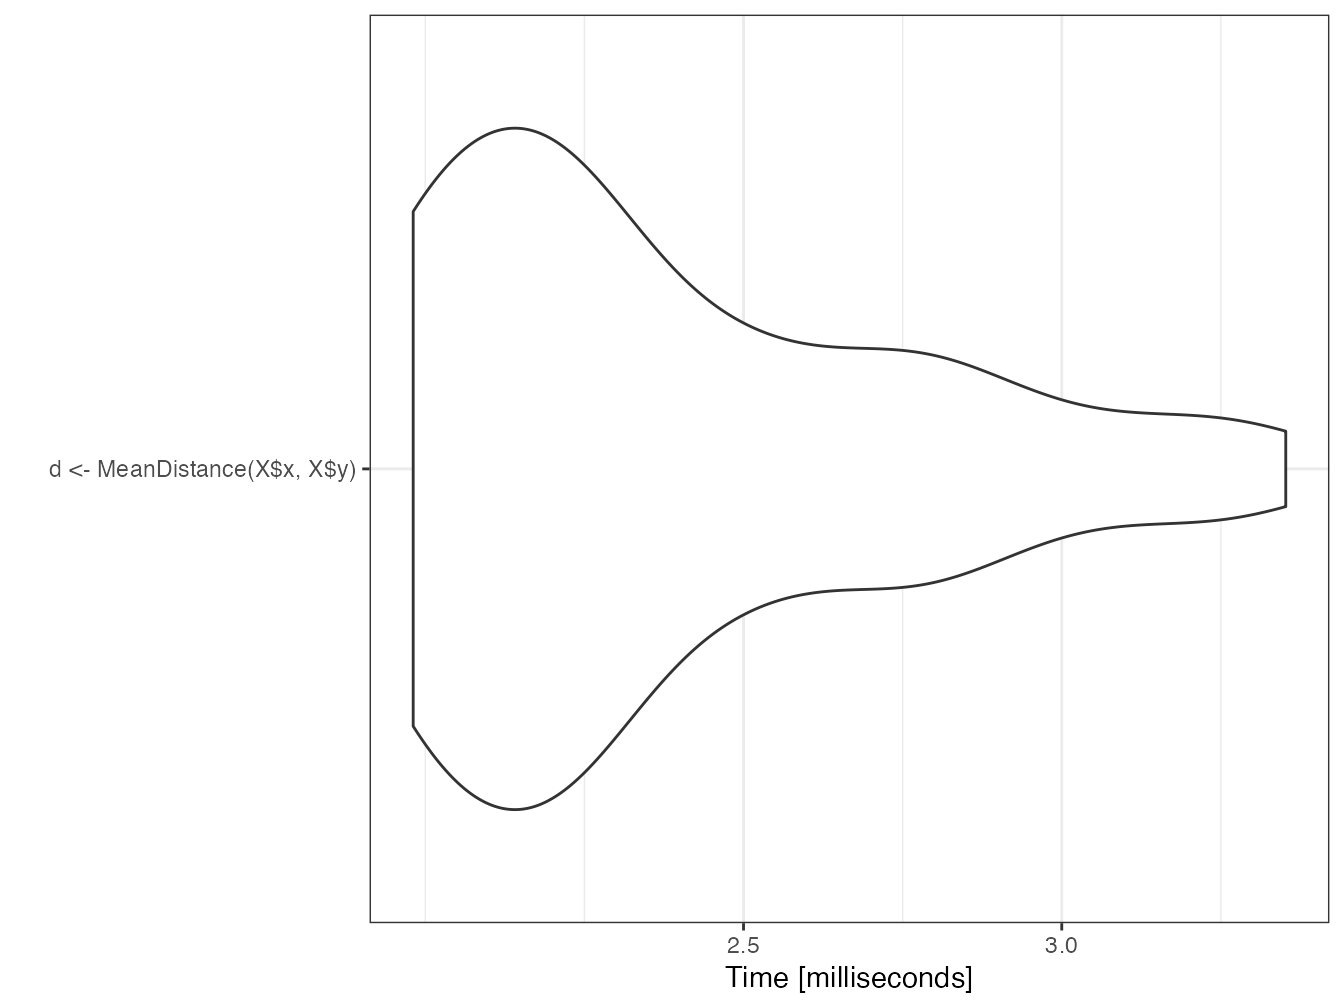
\includegraphics[width=0.8\linewidth]{travailleR_files/figure-latex/RCpp-1} \end{center}

\begin{Shaded}
\begin{Highlighting}[]
\NormalTok{d}
\end{Highlighting}
\end{Shaded}

\begin{verbatim}
## [1] 0.5154879
\end{verbatim}

\normalsize

\subsection{RcppParallel}\label{rcppparallel}

\textbf{RcppParallel} permet d'interfacer du code C++ parallélisé, au prix d'une syntaxe plus complexe qu'avec \textbf{RCpp}.
Une documentation est disponible\footnote{\url{http://rcppcore.github.io/RcppParallel/}}.

La fonction C++ exportée dans R ne réalise pas les calculs mais organise seulement l'exécution en parallèle d'une autre fonction, non exportée, de type \texttt{Worker}.

Deux fonctions (C++) de parallélisation sont disponibles pour deux types de tâches:

\begin{itemize}
\tightlist
\item
  \texttt{parallelReduce} pour l'accumulation d'une valeur, utilisée ici pour additionner les distances.
\item
  \texttt{parallelFor} pour remplir une matrice de résultats.
\end{itemize}

La syntaxe du \texttt{Worker} est un peu laborieuse mais assez simple à adapter: les constructeurs initialisent les variables C à partir des valeurs transmises par R et déclarent la parallélisation.

\scriptsize

\begin{Shaded}
\begin{Highlighting}[]
\CommentTok{// [[Rcpp::depends(RcppParallel)]]}
\PreprocessorTok{\#include }\ImportTok{\textless{}Rcpp.h\textgreater{}}
\PreprocessorTok{\#include }\ImportTok{\textless{}RcppParallel.h\textgreater{}}
\KeywordTok{using} \KeywordTok{namespace}\NormalTok{ Rcpp}\OperatorTok{;}
\KeywordTok{using} \KeywordTok{namespace}\NormalTok{ RcppParallel}\OperatorTok{;}

\CommentTok{// Working function, not exported}
\KeywordTok{struct}\NormalTok{ TotalDistanceWrkr }\OperatorTok{:} \KeywordTok{public}\NormalTok{ Worker}
\OperatorTok{\{}
  \CommentTok{// source vectors}
  \AttributeTok{const}\NormalTok{ RVector}\OperatorTok{\textless{}}\DataTypeTok{double}\OperatorTok{\textgreater{}}\NormalTok{ Rx}\OperatorTok{;}
  \AttributeTok{const}\NormalTok{ RVector}\OperatorTok{\textless{}}\DataTypeTok{double}\OperatorTok{\textgreater{}}\NormalTok{ Ry}\OperatorTok{;}
  
  \CommentTok{// accumulated value}
  \DataTypeTok{double}\NormalTok{ distance}\OperatorTok{;}
   
  \CommentTok{// constructors}
\NormalTok{  TotalDistanceWrkr}\OperatorTok{(}\AttributeTok{const}\NormalTok{ NumericVector x}\OperatorTok{,} \AttributeTok{const}\NormalTok{ NumericVector y}\OperatorTok{)} \OperatorTok{:}
\NormalTok{    Rx}\OperatorTok{(}\NormalTok{x}\OperatorTok{),}\NormalTok{ Ry}\OperatorTok{(}\NormalTok{y}\OperatorTok{),}\NormalTok{ distance}\OperatorTok{(}\DecValTok{0}\OperatorTok{)} \OperatorTok{\{\}}
\NormalTok{  TotalDistanceWrkr}\OperatorTok{(}\AttributeTok{const}\NormalTok{ TotalDistanceWrkr}\OperatorTok{\&}\NormalTok{ totalDistanceWrkr}\OperatorTok{,}\NormalTok{ Split}\OperatorTok{)} \OperatorTok{:}
\NormalTok{    Rx}\OperatorTok{(}\NormalTok{totalDistanceWrkr}\OperatorTok{.}\NormalTok{Rx}\OperatorTok{),}\NormalTok{ Ry}\OperatorTok{(}\NormalTok{totalDistanceWrkr}\OperatorTok{.}\NormalTok{Ry}\OperatorTok{),}\NormalTok{  distance}\OperatorTok{(}\DecValTok{0}\OperatorTok{)} \OperatorTok{\{\}}
  
  \CommentTok{// count neighbors}
  \DataTypeTok{void} \KeywordTok{operator}\OperatorTok{()(}\BuiltInTok{std::}\NormalTok{size\_t begin}\OperatorTok{,} \BuiltInTok{std::}\NormalTok{size\_t end}\OperatorTok{)} \OperatorTok{\{}
    \DataTypeTok{double}\NormalTok{ dx}\OperatorTok{,}\NormalTok{ dy}\OperatorTok{;}
    \DataTypeTok{unsigned} \DataTypeTok{int}\NormalTok{ Npoints }\OperatorTok{=}\NormalTok{ Rx}\OperatorTok{.}\NormalTok{length}\OperatorTok{();}

    \ControlFlowTok{for} \OperatorTok{(}\DataTypeTok{unsigned} \DataTypeTok{int}\NormalTok{ i }\OperatorTok{=}\NormalTok{ begin}\OperatorTok{;}\NormalTok{ i }\OperatorTok{\textless{}}\NormalTok{ end}\OperatorTok{;}\NormalTok{ i}\OperatorTok{++)} \OperatorTok{\{}
      \ControlFlowTok{for} \OperatorTok{(}\DataTypeTok{unsigned} \DataTypeTok{int}\NormalTok{ j }\OperatorTok{=}\NormalTok{ i }\OperatorTok{+} \DecValTok{1}\OperatorTok{;}\NormalTok{ j }\OperatorTok{\textless{}}\NormalTok{ Npoints}\OperatorTok{;}\NormalTok{ j}\OperatorTok{++)} \OperatorTok{\{}
          \CommentTok{// Calculate squared distance}
\NormalTok{          dx }\OperatorTok{=}\NormalTok{ Rx}\OperatorTok{[}\NormalTok{i}\OperatorTok{]} \OperatorTok{{-}}\NormalTok{ Rx}\OperatorTok{[}\NormalTok{j}\OperatorTok{];}
\NormalTok{          dy }\OperatorTok{=}\NormalTok{ Ry}\OperatorTok{[}\NormalTok{i}\OperatorTok{]} \OperatorTok{{-}}\NormalTok{ Ry}\OperatorTok{[}\NormalTok{j}\OperatorTok{];}
\NormalTok{          distance }\OperatorTok{+=}\NormalTok{ sqrt}\OperatorTok{(}\NormalTok{dx }\OperatorTok{*}\NormalTok{ dx }\OperatorTok{+}\NormalTok{ dy }\OperatorTok{*}\NormalTok{ dy}\OperatorTok{);}
      \OperatorTok{\}}
    \OperatorTok{\}}
  \OperatorTok{\}}

  \CommentTok{// join my value with that of another Sum}
  \DataTypeTok{void}\NormalTok{ join}\OperatorTok{(}\AttributeTok{const}\NormalTok{ TotalDistanceWrkr}\OperatorTok{\&}\NormalTok{ rhs}\OperatorTok{)} \OperatorTok{\{} 
\NormalTok{    distance }\OperatorTok{+=}\NormalTok{ rhs}\OperatorTok{.}\NormalTok{distance}\OperatorTok{;} 
  \OperatorTok{\}}
\OperatorTok{\};}


\CommentTok{// Exported function}
\CommentTok{// [[Rcpp::export]]}
\DataTypeTok{double}\NormalTok{ TotalDistance}\OperatorTok{(}\NormalTok{NumericVector x}\OperatorTok{,}\NormalTok{ NumericVector y}\OperatorTok{)} \OperatorTok{\{}
  
  \CommentTok{// Declare TotalDistanceWrkr instance}
\NormalTok{  TotalDistanceWrkr totalDistanceWrkr}\OperatorTok{(}\NormalTok{x}\OperatorTok{,}\NormalTok{ y}\OperatorTok{);}
  
  \CommentTok{// call parallel\_reduce to start the work}
\NormalTok{  parallelReduce}\OperatorTok{(}\DecValTok{0}\OperatorTok{,}\NormalTok{ x}\OperatorTok{.}\NormalTok{length}\OperatorTok{(),}\NormalTok{ totalDistanceWrkr}\OperatorTok{);}
  
  \CommentTok{// return the result}
  \ControlFlowTok{return}\NormalTok{ totalDistanceWrkr}\OperatorTok{.}\NormalTok{distance}\OperatorTok{;}
\OperatorTok{\}}
\end{Highlighting}
\end{Shaded}

\normalsize

L'usage dans R est identique à celui des fonctions C++ interfacées par \textbf{RCpp}.

\scriptsize

\begin{Shaded}
\begin{Highlighting}[]
\NormalTok{(mb }\OtherTok{\textless{}{-}} \FunctionTok{microbenchmark}\NormalTok{(}
\NormalTok{  d }\OtherTok{\textless{}{-}} \FunctionTok{TotalDistance}\NormalTok{(X}\SpecialCharTok{$}\NormalTok{x, X}\SpecialCharTok{$}\NormalTok{y) }\SpecialCharTok{/}\NormalTok{ NbPoints }\SpecialCharTok{/}\NormalTok{ (NbPoints }\SpecialCharTok{{-}} \DecValTok{1}\NormalTok{) }\SpecialCharTok{*} \DecValTok{2}\NormalTok{)}
\NormalTok{)}
\end{Highlighting}
\end{Shaded}

\begin{verbatim}
## Unit: microseconds
##                                                      expr
##  d <- TotalDistance(X$x, X$y)/NbPoints/(NbPoints - 1) * 2
##      min       lq     mean  median       uq      max neval
##  219.145 221.4205 269.7898 232.347 239.9525 3258.598   100
\end{verbatim}

\begin{Shaded}
\begin{Highlighting}[]
\FunctionTok{autoplot}\NormalTok{(mb)}
\end{Highlighting}
\end{Shaded}

\begin{center}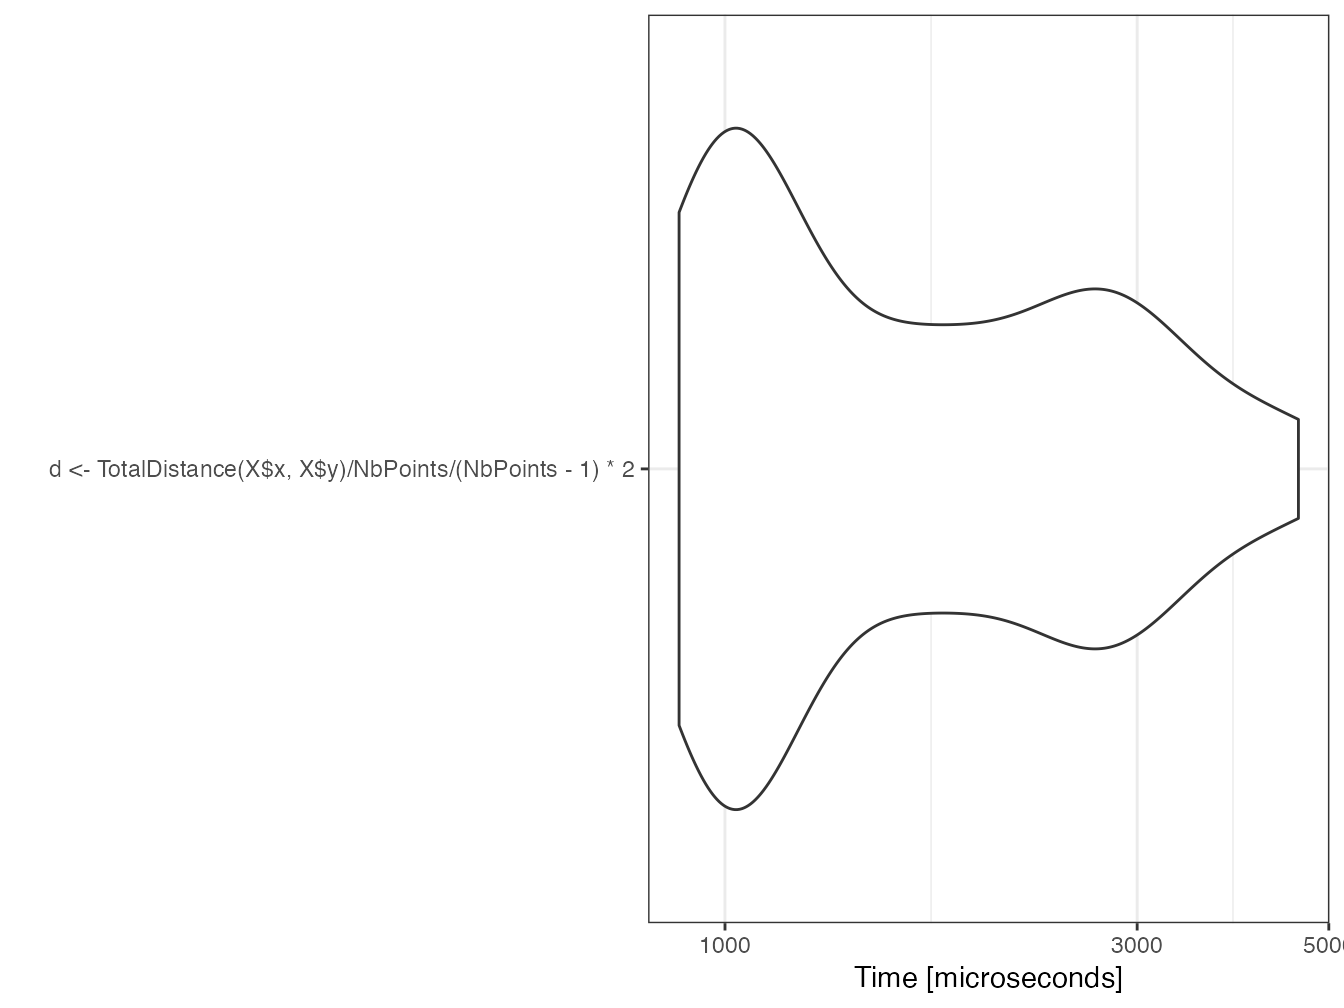
\includegraphics[width=0.8\linewidth]{travailleR_files/figure-latex/RcppParallel-1} \end{center}

\begin{Shaded}
\begin{Highlighting}[]
\NormalTok{d}
\end{Highlighting}
\end{Shaded}

\begin{verbatim}
## [1] 0.5154879
\end{verbatim}

\normalsize

Le temps de mise en place des tâches parallèles est bien plus long que le temps de calcul en série.

En multipliant le nombre de points par 50, le temps de calcul en série doit être multiplié par 2500 environ.

\scriptsize

\begin{Shaded}
\begin{Highlighting}[]
\NormalTok{NbPoints }\OtherTok{\textless{}{-}} \DecValTok{50000}
\NormalTok{X }\OtherTok{\textless{}{-}} \FunctionTok{runifpoint}\NormalTok{(NbPoints)}
\FunctionTok{system.time}\NormalTok{(d }\OtherTok{\textless{}{-}} \FunctionTok{MeanDistance}\NormalTok{(X}\SpecialCharTok{$}\NormalTok{x, X}\SpecialCharTok{$}\NormalTok{y))}
\end{Highlighting}
\end{Shaded}

\begin{verbatim}
##    user  system elapsed 
##   4.319   0.005   4.326
\end{verbatim}

\normalsize

En parallèle, le temps augmente peu: la parallélisation devient réellement efficace.
Ce temps est à comparer à celui de la boucle for de référence, multiplié par 2500, soit \texttt{2032} secondes.

\scriptsize

\begin{Shaded}
\begin{Highlighting}[]
\FunctionTok{system.time}\NormalTok{(}
\NormalTok{  d }\OtherTok{\textless{}{-}} \FunctionTok{TotalDistance}\NormalTok{(X}\SpecialCharTok{$}\NormalTok{x, X}\SpecialCharTok{$}\NormalTok{y) }\SpecialCharTok{/}\NormalTok{ NbPoints }\SpecialCharTok{/}\NormalTok{ (NbPoints }\SpecialCharTok{{-}} \DecValTok{1}\NormalTok{) }\SpecialCharTok{*} \DecValTok{2}
\NormalTok{)}
\end{Highlighting}
\end{Shaded}

\begin{verbatim}
##    user  system elapsed 
##   1.269   0.004   0.442
\end{verbatim}

\normalsize

\subsection{Conclusions sur l'optimisation de la vitesse du code}\label{conclusions-sur-loptimisation-de-la-vitesse-du-code}

De cette étude de cas, plusieurs enseignements peuvent être retirés:

\begin{itemize}
\tightlist
\item
  une boucle for est une bonne base pour des calculs répétitifs, plus rapide que \texttt{vapply()}, simple à lire et à écrire;
\item
  les boucles \textbf{foreach} sont extrêmement efficaces pour paralléliser des boucles for;
\item
  des fonctions optimisées peuvent exister dans les packages de R pour des tâches courantes (ici, la fonction \texttt{pairdist()} de \textbf{spatstat} est deux ordres de grandeur plus rapide que la boucle for);
\item
  le package \textbf{future.apply} permet de paralléliser très simplement du code déjà écrit avec des fonctions \texttt{*apply()}, indépendamment du matériel utilisé;
\item
  le recours au code C++ permet d'accélérer significativement les calculs, de trois ordres de grandeur ici;
\item
  la parallélisation du code C++ divise encore le temps de calcul par environ la moitié du nombre de cœurs pour de longs calculs.
\end{itemize}

Au-delà de cet exemple, l'optimisation du temps de calcul sous R peut être compliquée si elle passe par la parallélisation et l'écriture de code C++.
L'effort doit donc être concentré sur les calculs réellement long alors que la lisibilité du code doit rester la priorité pour le code courant.
Le code C est assez facile à intégrer grâce à \textbf{RCpp} et sa parallélisation n'est pas très coûteuse avec \textbf{RCppParallel}.

L'utilisation de boucles for n'est plus pénalisante depuis la version 3.5 de R.
L'écriture de code vectoriel, utilisant \texttt{sapply()} se justifie toujours pour sa lisibilité.

Le choix de paralléliser le code doit être évalué selon le temps d'exécution de chaque tâche parallélisable.
S'il dépasse quelques secondes, la parallélisation se justifie.

\section{Flux de travail}\label{sec:targets}

Le package \textbf{targets} permet de gérer un flux de travail (\emph{workflow}), c'est-à dire de décomposer le code en tâches élémentaires appelées \emph{cibles} qui s'enchaînent, dont le résultat est stocké dans une variable, elle-même enregistrée sur le disque.
En cas de changement dans le code ou les données utilisées, seules les cibles concernées sont réévaluées.

Le fonctionnement du flux est proche de celui d'un cache, mais ne dépend pas de l'ordinateur sur lequel il s'exécute.
\textbf{targets} permet de visualiser les tâches obsolètes, d'intégrer le flux à un projet de document (voir section \ref{sec:targetsmd}), et même de faire appel à un cluster de calcul pour traiter les tâches en parallèle.

\subsection{Principe de fonctionnement}\label{principe-de-fonctionnement}

La documentation\footnote{\url{https://books.ropensci.org/targets/}} de \textbf{targets} est détaillée et fournit un exemple travaillé pour apprendre à utiliser le package\footnote{\url{https://books.ropensci.org/targets/walkthrough.html}}.
Elle n'est pas reprise ici, mais les principes du fonctionnement du flux sont expliqués.

Le flux de travail est unique pour un projet donné.
Il est codé dans le fichier \texttt{\_targets.R} à la racine du projet.
Il contient:

\begin{itemize}
\tightlist
\item
  des commandes globales, comme le chargement des packages;
\item
  une liste de cibles, qui décrivent le code à exécuter et la variable qui stocke leur résultat.
\end{itemize}

Le flux est exécuté par la fonction \texttt{tar\_make()} qui met à jour les cibles qui le nécessitent.
Son contenu est placé dans le dossier \texttt{\_targets}.
Les variables stockées sont lues par \texttt{tar\_read()}.

Si le projet nécessite de longs calculs, \textbf{targets} permet de n'exécuter que ceux qui sont nécessaires.
Si le projet est partagé ou placé sous contrôle de source (chapitre \ref{chap-git}), le résultat des calcul est intégré l'est aussi.
Enfin, si le projet est un document (chapitre \ref{chap-rediger}), son formatage est complètement indépendant du calcul de son contenu, pour un gain de temps qui peut être considérable.

\subsection{Exemple minimal}\label{exemple-minimal}

L'exemple suivant est encore plus simple que celui du manuel de \textbf{targets}, qui permettra d'aller plus loin.
Il reprend l'étude de cas précédente: un jeu de points est généré puis la distance moyenne entre les points obtenus est calculée.
Une carte des points est tracée en plus.
Chacune de ces trois opérations est une cible dans le vocabulaire de \textbf{targets}.

Le fichier du flux de travail est donc le suivant:

\scriptsize

\begin{Shaded}
\begin{Highlighting}[]
\CommentTok{\# Fichier \_targets.R }
\FunctionTok{library}\NormalTok{(}\StringTok{"targets"}\NormalTok{)}
\FunctionTok{tar\_option\_set}\NormalTok{(}\AttributeTok{packages =} \FunctionTok{c}\NormalTok{(}\StringTok{"spatstat"}\NormalTok{, }\StringTok{"dbmss"}\NormalTok{))}
\FunctionTok{list}\NormalTok{(}
  \CommentTok{\# Tirage des points}
  \FunctionTok{tar\_target}\NormalTok{(X,}
    \FunctionTok{runifpoint}\NormalTok{(NbPoints)}
\NormalTok{  ),}
  \CommentTok{\# Paramétrage}
  \FunctionTok{tar\_target}\NormalTok{(NbPoints,}
    \DecValTok{1000}
\NormalTok{  ),}
  \CommentTok{\# Distance moyenne}
  \FunctionTok{tar\_target}\NormalTok{(d,}
    \FunctionTok{sum}\NormalTok{(}\FunctionTok{pairdist}\NormalTok{(X)) }\SpecialCharTok{/}\NormalTok{ NbPoints }\SpecialCharTok{/}\NormalTok{ (NbPoints }\SpecialCharTok{{-}} \DecValTok{1}\NormalTok{)}
\NormalTok{  ),}
  \CommentTok{\# Carte}
  \FunctionTok{tar\_target}\NormalTok{(map, }
    \FunctionTok{autoplot}\NormalTok{(}\FunctionTok{as.wmppp}\NormalTok{(X))}
\NormalTok{  )}
\NormalTok{)}
\end{Highlighting}
\end{Shaded}

\normalsize

Les commandes globales consistent à charger le package \textbf{targets} lui-même puis lister les packages nécessaires au code.
L'exécution du flux a lieu dans une nouvelle instance de R.

Les cibles sont ensuite listées.
Chacune est déclarée par la fonction \texttt{tar\_target()} dont le premier argument est le nom de la cible, qui sera celui de la variable qui recevra le résultat.
Le deuxième argument est le code qui produit le résultat.
Les cibles sont très simples ici et peuvent être écrites en une seule commande.
Quand ce n'est pas le cas, chaque cible peut être écrite sous la forme d'une fonction, stockée dans un fichier de code séparé chargé par la fonction \texttt{source()} au début du fichier de flux.

La commande \texttt{tar\_visnetwork} permet d'afficher l'enchaînement des cibles et leur état éventuellement obsolète.

\scriptsize

\begin{Shaded}
\begin{Highlighting}[]
\FunctionTok{library}\NormalTok{(}\StringTok{"targets"}\NormalTok{)}
\FunctionTok{tar\_visnetwork}\NormalTok{()}
\end{Highlighting}
\end{Shaded}

\normalsize

L'ordre de déclaration des cibles dans la liste sans importance: elles sont ordonnées automatiquement.

Le flux est exécuté par \texttt{tar\_make()}.

\scriptsize

\begin{Shaded}
\begin{Highlighting}[]
\FunctionTok{tar\_make}\NormalTok{()}
\end{Highlighting}
\end{Shaded}

\begin{verbatim}
## ▶ dispatched target NbPoints
## ● completed target NbPoints [0.644 seconds, 53 bytes]
## ▶ dispatched target X
## ● completed target X [0.002 seconds, 11.058 kilobytes]
## ▶ dispatched target d
## ● completed target d [0.007 seconds, 55 bytes]
## ▶ dispatched target map
## ● completed target map [0.015 seconds, 187.39 kilobytes]
## ▶ ended pipeline [0.768 seconds]
\end{verbatim}

\normalsize

Le flux est maintenant à jour et \texttt{tar\_make()} ne refait aucun calcul.

\scriptsize

\begin{Shaded}
\begin{Highlighting}[]
\FunctionTok{tar\_visnetwork}\NormalTok{()}
\end{Highlighting}
\end{Shaded}

\begin{Shaded}
\begin{Highlighting}[]
\FunctionTok{tar\_make}\NormalTok{()}
\end{Highlighting}
\end{Shaded}

\begin{verbatim}
## ✔ skipping targets (1 so far)...
## ✔ skipped pipeline [0.035 seconds]
\end{verbatim}

\normalsize

Les résultats sont lus par \texttt{tar\_read()}.

\scriptsize

\begin{Shaded}
\begin{Highlighting}[]
\FunctionTok{tar\_read}\NormalTok{(d)}
\end{Highlighting}
\end{Shaded}

\begin{verbatim}
## [1] 0.5165293
\end{verbatim}

\begin{Shaded}
\begin{Highlighting}[]
\FunctionTok{tar\_read}\NormalTok{(map)}
\end{Highlighting}
\end{Shaded}

\begin{center}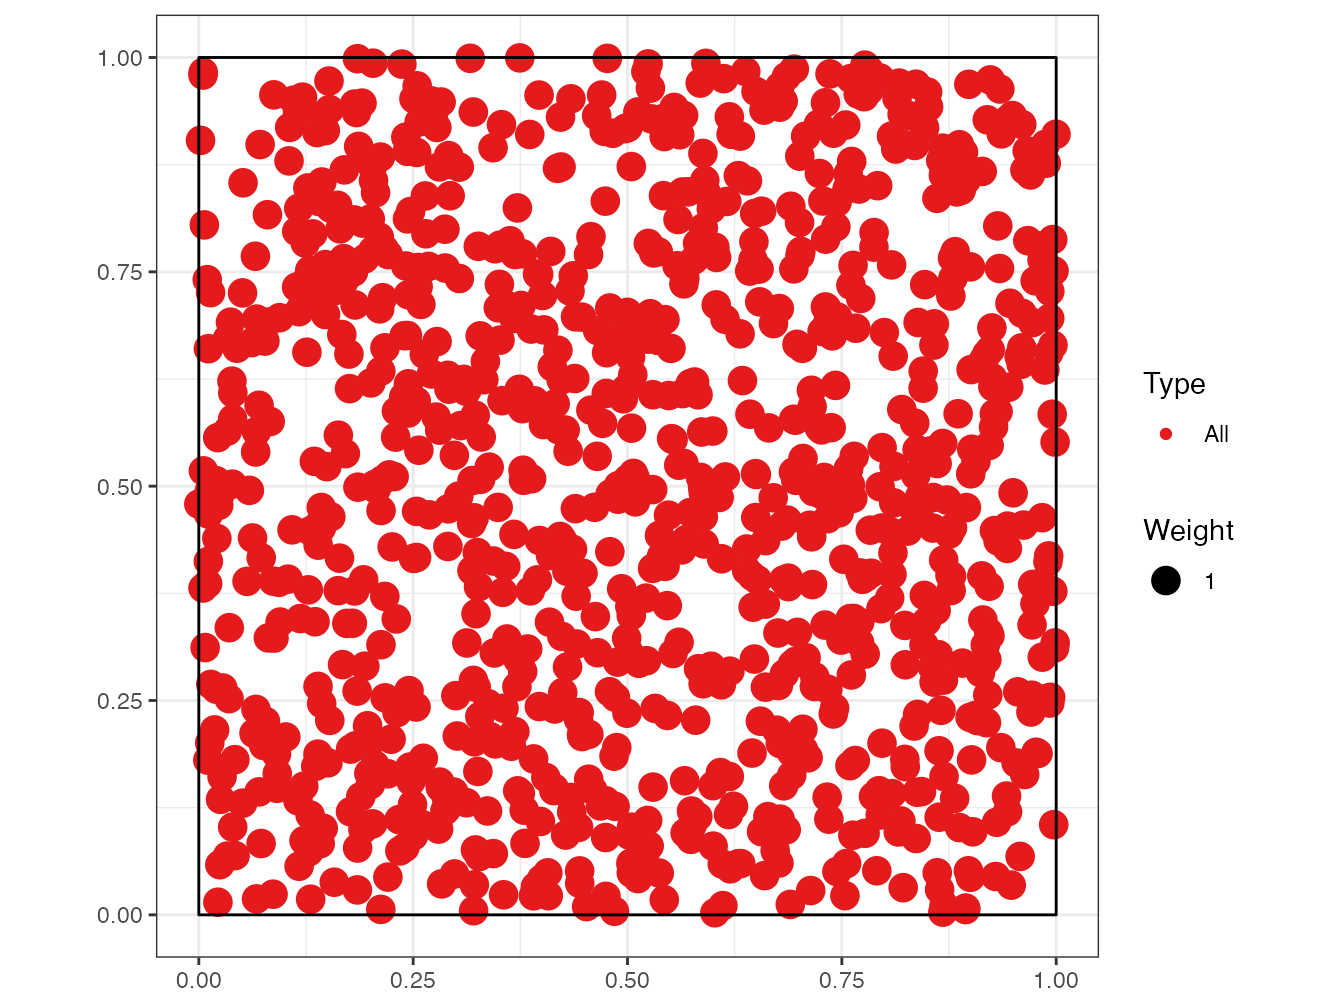
\includegraphics[width=0.8\linewidth]{travailleR_files/figure-latex/tar_read-1} \end{center}

\normalsize

\subsection{Intérêt pratique}\label{intuxe9ruxeat-pratique}

Dans cet exemple, \textbf{targets} complique l'écriture du code et \texttt{tar\_make()} est beaucoup plus lent que la simple exécution du code qu'il traite parce qu'il doit vérifier si les cibles sont à jour.
Dans un projet réel qui nécessite de longs calculs, le traitement du statut des cibles est négligeable et le gain de temps apporté par la seule évaluation des cibles nécessaires est considérable.
La définition des cibles reste une contrainte, mais force à bien structurer son projet.

\chapter{Git et GitHub}\label{chap-git}

\toc{1}

Le contrôle de source consiste à enregistrer l'ensemble des modifications apportées sur les fichiers suivis.
Les avantages sont nombreux: traçabilité et sécurité du projet, possibilité de collaborer efficacement, de revenir en arrière, de tenter de nouveaux développements sans mettre en péril la version stable\ldots{}

\section{Principes}\label{sec:principes-git}

\subsection{Contrôle de source}\label{sec:git-cds}

L'outil standard est aujourd'hui \emph{git}.

Les commandes de git peuvent être exécutées dans le terminal de RStudio.



\scriptsize

\begin{figure}

{\centering 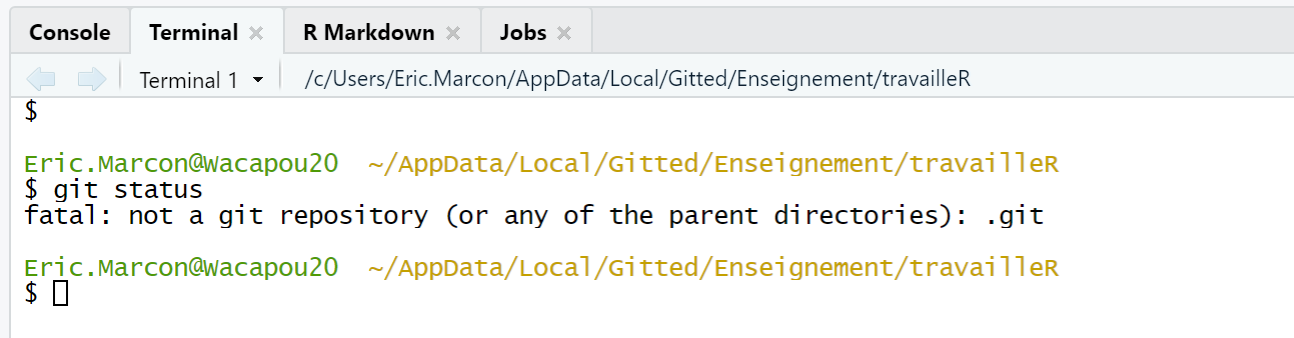
\includegraphics[width=0.8\linewidth]{images/git-Status} 

}

\caption{Capture d'écran du terminal de RStudio. La commande \texttt{git\ status} supposée décrire l'état du dépôt renvoie une erreur si le projet R n'est pas sous contrôle de source.}\label{fig:git-Status}
\end{figure}

\normalsize

La commande \texttt{git\ status} (figure \ref{fig:git-Status}) retourne l'état du dépôt (\emph{repository}), c'est-à-dire l'ensemble des données gérées par git pour suivre le projet en cours.

RStudio intègre une interface graphique pour git suffisante pour se passer de la ligne de commande dans le cadre d'une utilisation standard, présentée ici.

\subsection{git et GitHub}\label{git-et-github-1}

\emph{git} est le logiciel installé sur le poste de travail.

\emph{GitHub} est une plateforme, accessible par le web\footnote{\url{https://github.com/}}, qui permet de partager le contenu des dépôts git (pour travailler à plusieurs) et de partager de la documentation sous la forme d'un site web (\emph{GitHub Pages}).

Comme GitHub permet au minimum la sauvegarde des dépôts git, les deux sont toujours utilisés ensemble.
GitHub n'est pas la seule plateforme utilisable mais la principale.
Les alternatives sont Bitbucket\footnote{\url{https://bitbucket.org/}} et GitLab\footnote{\url{https://about.gitlab.com/}} par exemple.

\section{Créer un nouveau dépôt}\label{sec:creerdepot}

\subsection{A partir d'un projet existant}\label{a-partir-dun-projet-existant}

Dans un projet R existant, activer le contrôle de source dans les options du projet (figure \ref{fig:git-Project}).
La commande exécutée est \texttt{git\ init}.
Redémarrer RStudio à la demande.



\scriptsize

\begin{figure}

{\centering 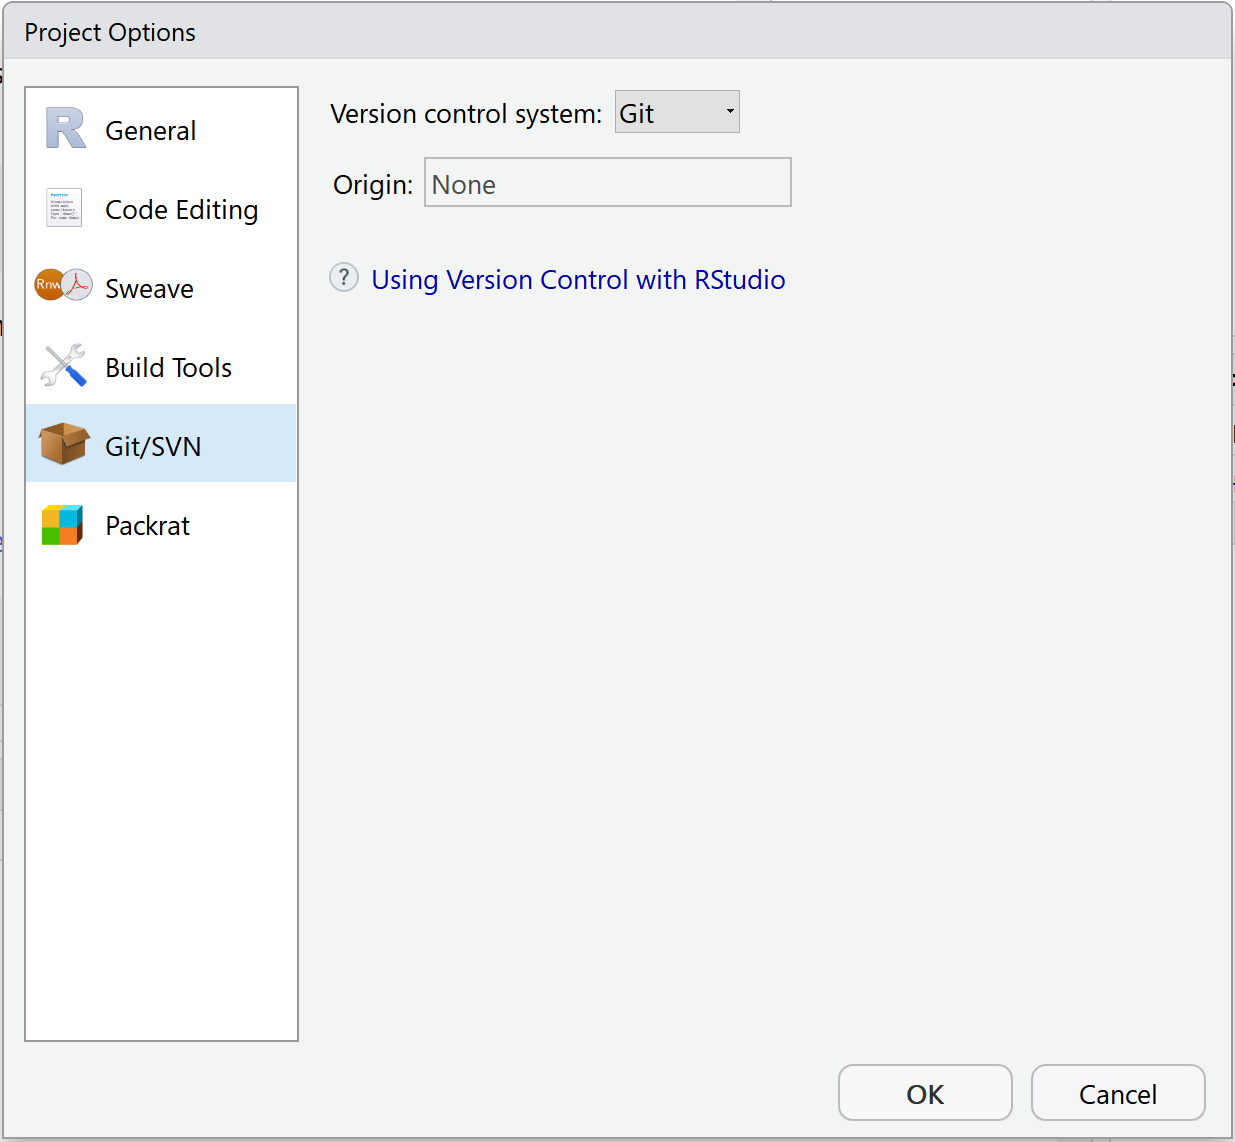
\includegraphics[width=0.8\linewidth]{images/git-Project} 

}

\caption{Activation du contrôle de source dans le menu \enquote{Tools \textgreater{} Project Options\ldots{}}.}\label{fig:git-Project}
\end{figure}

\normalsize

Une nouvelle fenêtre \emph{Git} apparaît dans le panneau supérieur droit.
Elle contient la liste des fichiers du projet (figure \ref{fig:git-Fichiers}).



\scriptsize

\begin{figure}

{\centering 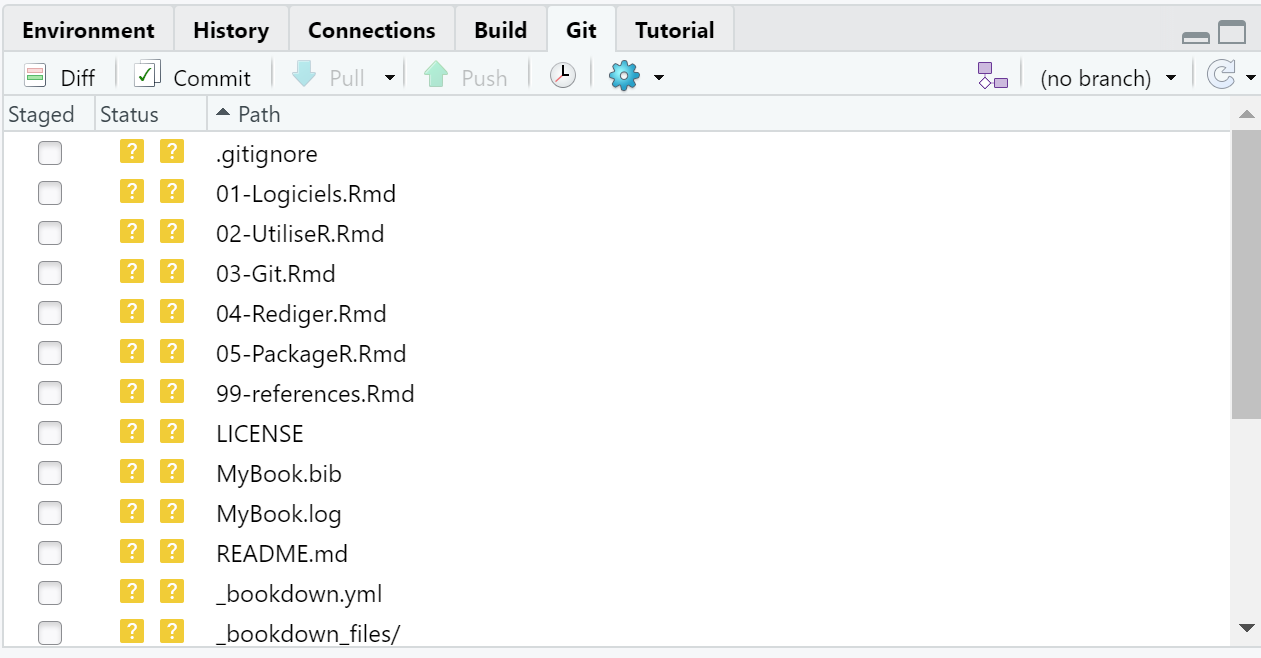
\includegraphics[width=0.8\linewidth]{images/git-Fichiers} 

}

\caption{Fichiers du projet, pas encore pris en compte par git.}\label{fig:git-Fichiers}
\end{figure}

\normalsize

A ce stade, les fichiers ne sont pas pris en compte par git: leur statut est un double point d'interrogation jaune.
Pour git, le répertoire de travail local est un \emph{bac à sable} où toutes les modifications sont possibles sans conséquences.

Le fichier \texttt{.gitignore} contient la liste des fichiers qui n'ont jamais vocation à être pris en compte, qu'il est donc inutile d'afficher dans la liste: les fichiers intermédiaires produits automatiquement par exemple.
La syntaxe des fichiers \texttt{.gitignore} est détaillée dans la documentation de git\footnote{\url{https://git-scm.com/docs/gitignore}}.
En règle générale, utiliser un fichier existant: les modèles de documents notamment incluent leur fichier \texttt{.gitignore}.

\subsection{Prendre en compte des fichiers}\label{prendre-en-compte-des-fichiers}

Dans la fenêtre git, cocher la case \emph{Staged} permet de prendre en compte (\emph{Stage}) chaque fichier.
La commande exécutée est \texttt{git\ add\ \textless{}NomDeFichier\textgreater{}}.
Les fichiers pris en compte une première fois ont le statut \enquote{A} pour \enquote{Added}.

Les fichiers pris en compte font partie de l'\emph{index} de git.

\subsection{Valider des modifications}\label{valider-des-modifications}



\scriptsize

\begin{figure}

{\centering 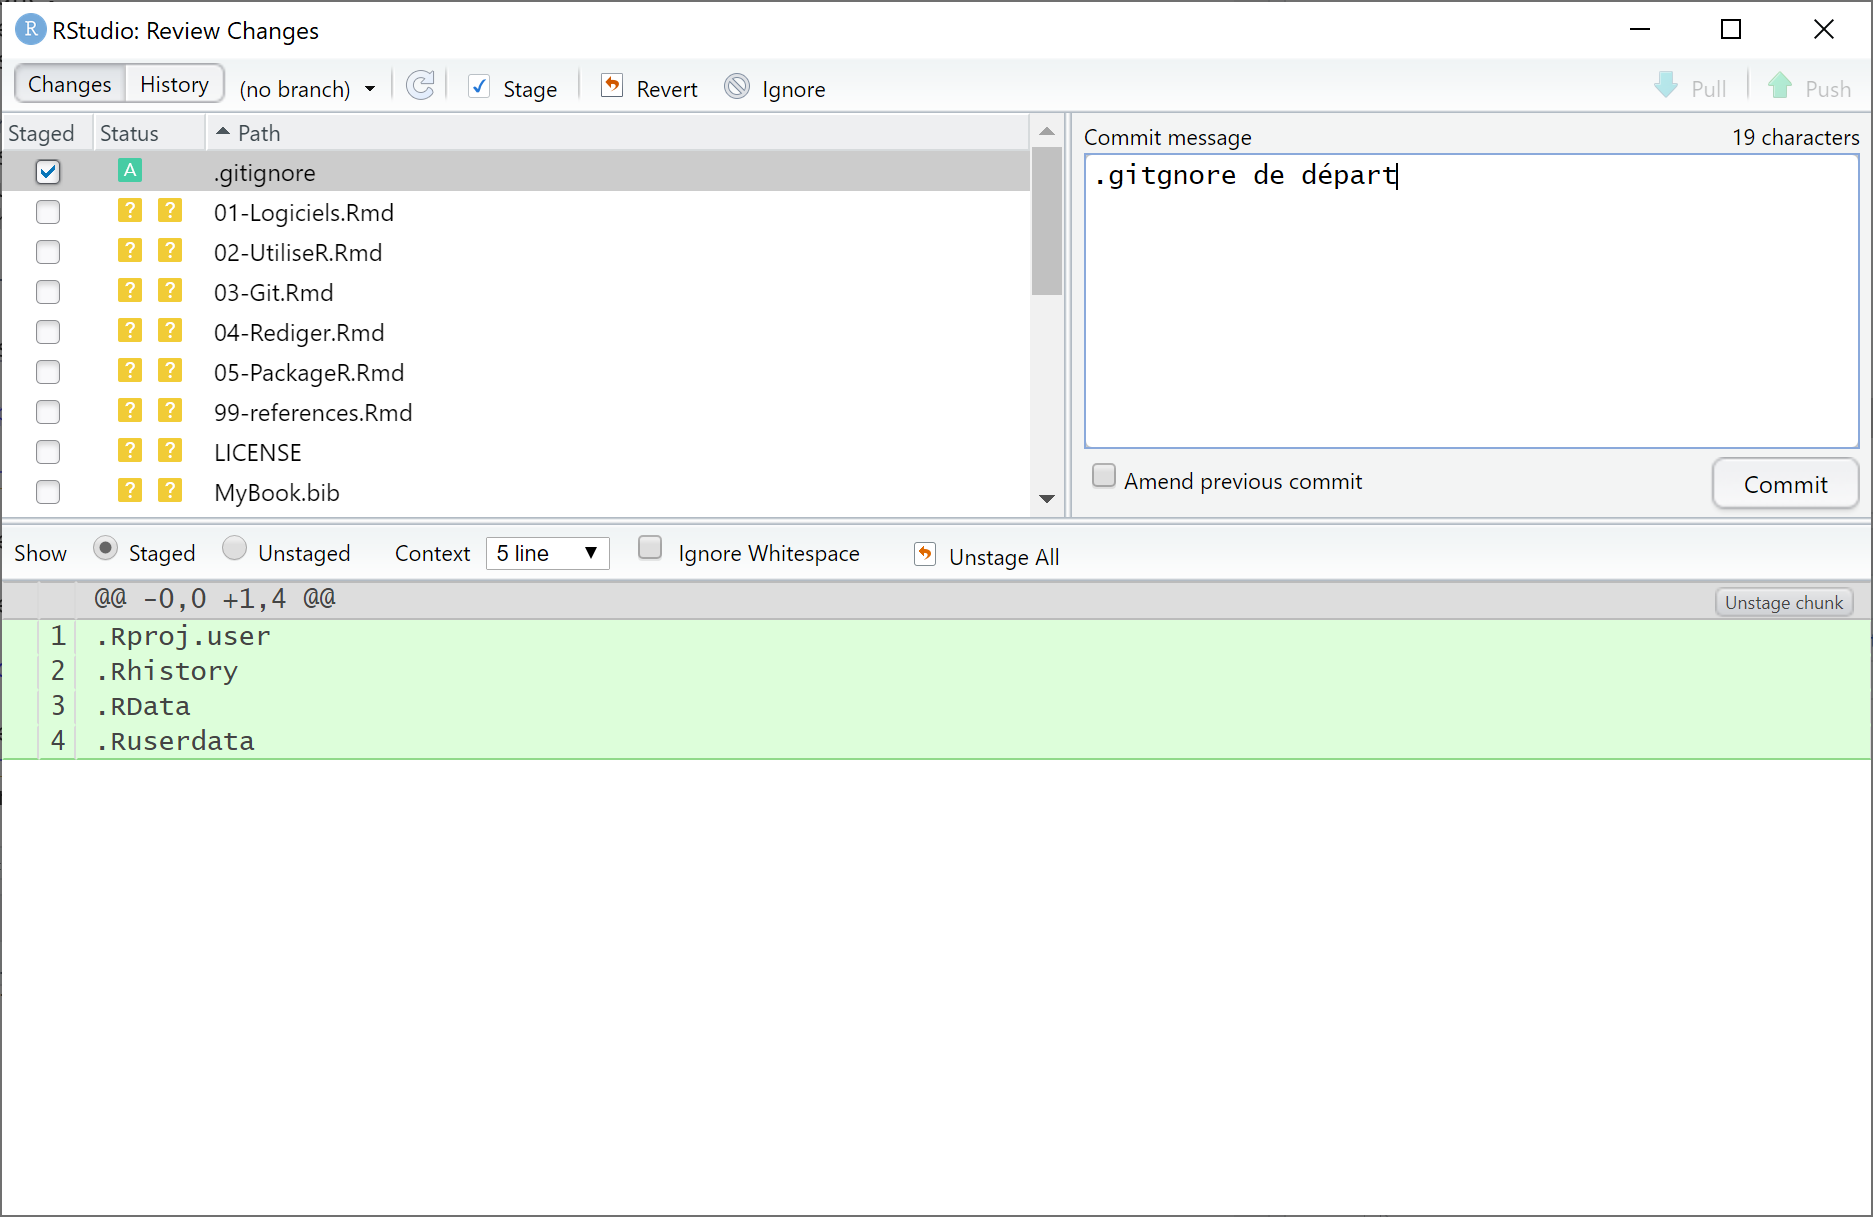
\includegraphics[width=0.8\linewidth]{images/git-Commit} 

}

\caption{Fenêtre de validation des modifications prises en compte.}\label{fig:git-Commit}
\end{figure}

\normalsize

Les fichiers pris en compte peuvent être validés (\emph{Commit}) en cliquant sur le bouton \enquote{Commit} dans la fenêtre \emph{Git}.
Une nouvelle fenêtre s'ouvre (figure \ref{fig:git-Commit}), qui permet de visualiser toutes les modifications par fichier (ajouts en verts, suppressions en rouge).
Le grain de modification traité par git est la ligne de texte, terminée par un retour à la ligne.
Les fichiers binaires comme les images sont traités en bloc.

Chaque validation (\emph{Commit}) est accompagnée d'un texte de description.
La première ligne est la description courte.
Une description détaillée peut être ajoutée après un saut de ligne.
Pour la lisibilité de l'historique du projet, chaque \emph{commit} correspond donc à une action, correspondant à la description courte: tous les fichiers modifiés ne sont pas forcément pris en compte et validés en une fois.
La commande exécutée est \texttt{git\ commit\ -m\ "Message\ de\ validation"}.



\scriptsize

\begin{figure}

{\centering 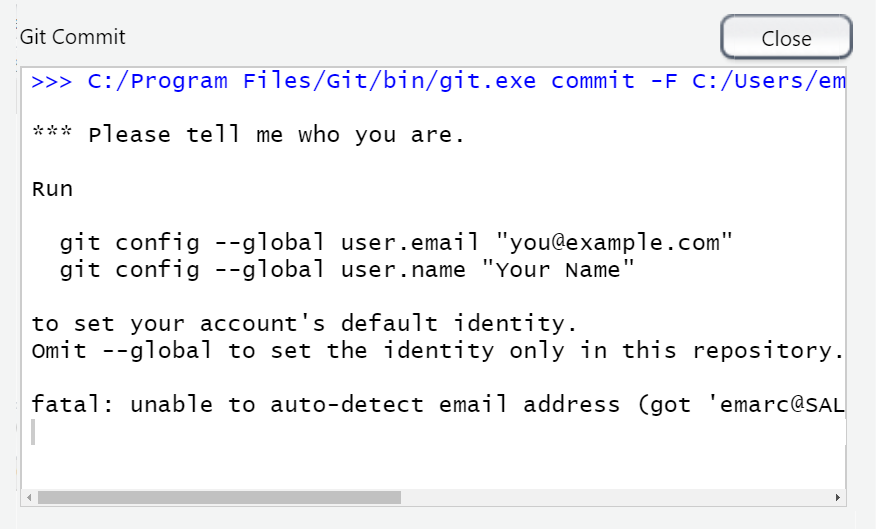
\includegraphics[width=0.8\linewidth]{images/git-id} 

}

\caption{Fenêtre de demande d'identification.}\label{fig:git-id}
\end{figure}

\normalsize

Les validations sont liées à leur auteur, qui doit être identifié par git.
En règle générale, git utilise les informations du système.
S'il n'y parvient pas, une fenêtre demande à l'utilisateur de s'identifier avant d'effectuer son premier \emph{commit} (figure \ref{fig:git-id}).
Les commandes indiquées sont à exécuter dans le terminal de RStudio.
Elles peuvent aussi être utilisées pour vérifier les valeurs connues par git:

\begin{verbatim}
git config user.name
git config user.email
\end{verbatim}

Dès la première validation, la branche principale du dépôt, appelée \enquote{master}, est créée.
Une branche est une version du dépôt, avec son propre historique et donc ses propres fichiers.
Les branches permettent:

\begin{itemize}
\tightlist
\item
  de développer de nouvelles fonctionnalités dans un projet, sans perturber la branche principale qui peut contenir une version stable.
  Si le développement est retenu, sa branche pourra être fusionnée avec la branche \emph{master} pour constituer une nouvelle version stable.
\item
  de contenir des fichiers totalement différents de ceux de la branche principale, pour d'autres objectifs.
  Sur GitHub, les pages web de présentation du projet peuvent être placés dans une branche appelée \enquote{gh-pages} qui ne sera jamais fusionnée.
\end{itemize}

Le dépôt git est complètement constitué.
Dans le vocabulaire de git, il comprend trois \emph{arbres} (figure \ref{fig:git-Trees}):

\begin{itemize}
\tightlist
\item
  le répertoire de travail, ou bac à sable, qui contient les fichiers non pris en compte: inconnus, modifiés, supprimés ou renommés (case \emph{Staged} décochée);
\item
  l'index, qui contient les fichiers pris en compte (case \emph{Staged} cochée);
\item
  la tête, qui contient les fichiers validés.
\end{itemize}



\scriptsize

\begin{figure}

{\centering 
\includegraphics[width=0.8\linewidth]{images/git-Trees} 

}

\caption{Les trois arbres de git. Source: \url{https://rogerdudler.github.io/git-guide/index.fr.html}}\label{fig:git-Trees}
\end{figure}

\normalsize

Le statut des fichiers est représenté par deux icônes dans la fenêtre \emph{Git} de RStudio: deux points d'interrogation quand ils n'ont pas été pris en compte par git.
Ensuite, l'icône de droite décrit la différence entre le le répertoire de travail et l'index.
Celle de gauche décrit la différence entre l'index et la tête.
Un fichier modifié aura donc l'icône \texttt{M} affichée à droite avant d'être pris en compte, puis à gauche après prise en compte.
Il est possible, même s'il vaut mieux l'éviter, de modifier à nouveau un fichier pris en compte avant qu'il soit validé: alors, les deux icônes seront affichées.

\subsection{Créer un dépôt vide sur GitHub}\label{cruxe9er-un-duxe9puxf4t-vide-sur-github}



\scriptsize

\begin{figure}

{\centering 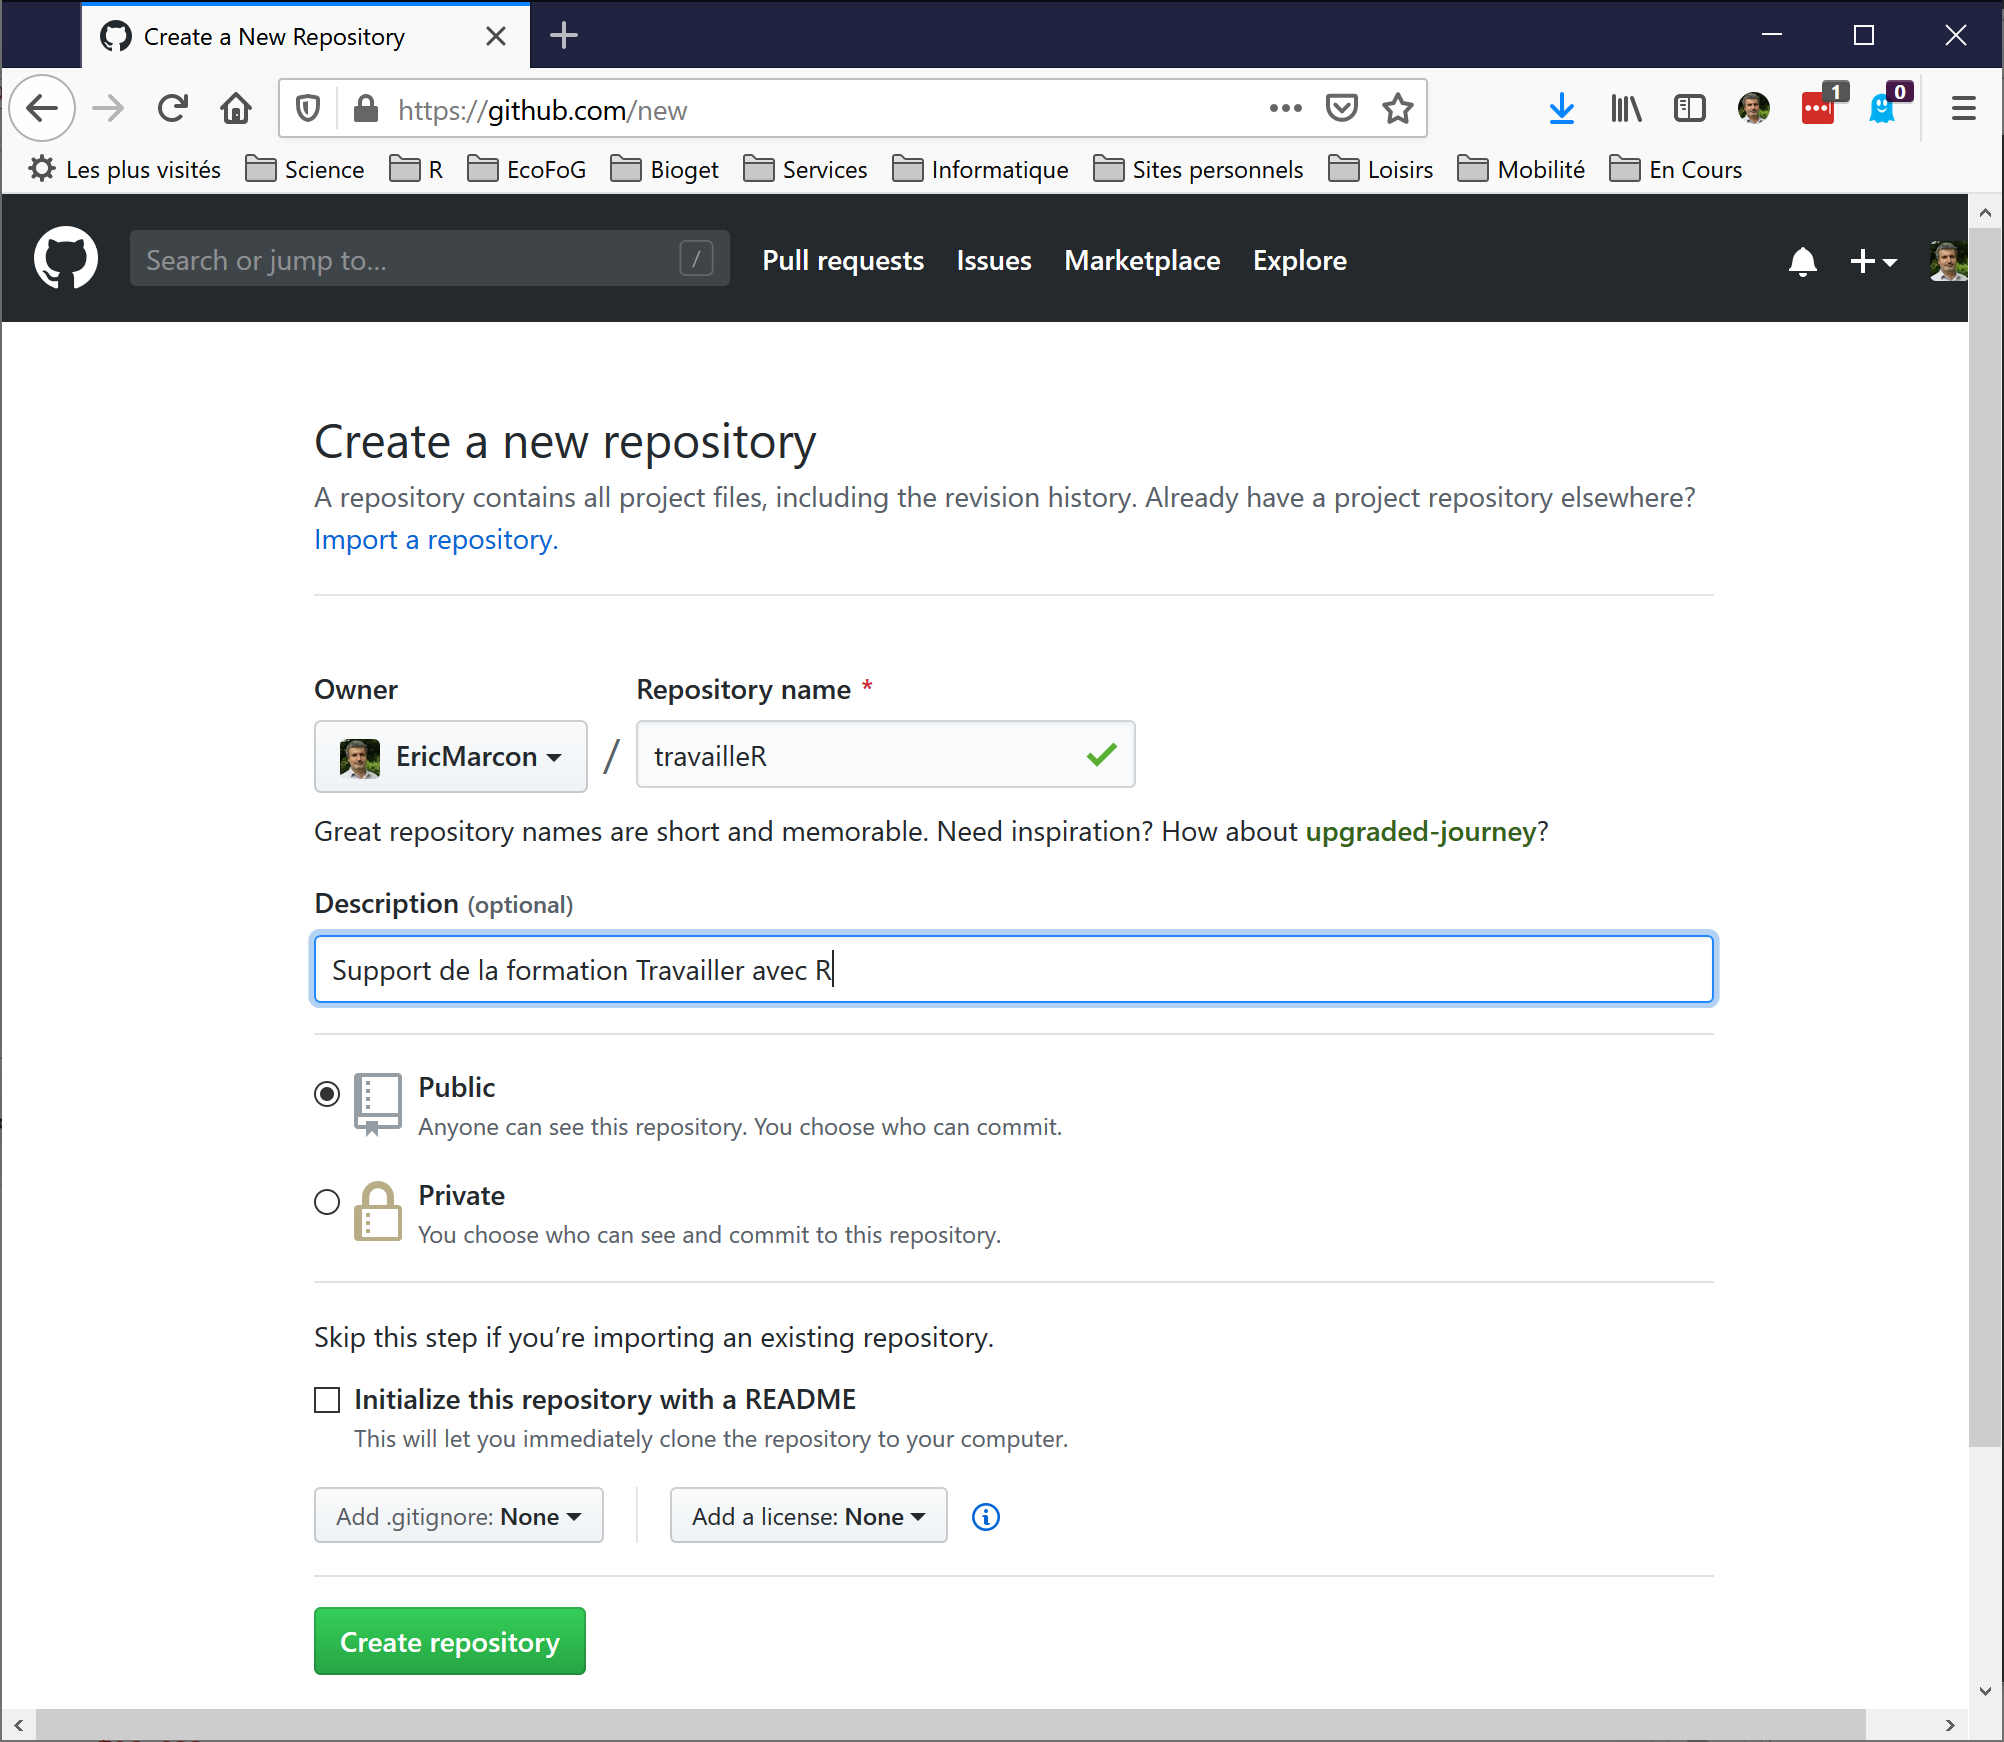
\includegraphics[width=0.8\linewidth]{images/CreateRepo} 

}

\caption{Création d'un dépôt sur GitHub.}\label{fig:CreateRepo}
\end{figure}

\normalsize

Un dépôt vide sur GitHub doit être créé (figure \ref{fig:CreateRepo}):

\begin{itemize}
\tightlist
\item
  sur GitHub, cliquer sur le bouton vert \enquote{New repository};
\item
  saisir le nom du dépôt, identique à celui du projet R local;
\item
  ajouter une description, qui apparaîtra uniquement sur la page GitHub du dépôt;
\item
  choisir le statut du dépôt:

  \begin{itemize}
  \tightlist
  \item
    public: visible par tout le monde;
  \item
    privé: visible seulement par les collaborateurs du projet, ce qui exclut de compléter par des pages web de présentation.
  \end{itemize}
\item
  ne pas ajouter de \texttt{README}, \texttt{.gitignore} ou licence: le projet doit être vide;
\item
  cliquer sur \enquote{create Repository};
\item
  copier l'adresse du dépôt (\url{https://github.com/}\ldots{} ou \href{mailto:git@github.com}{\nolinkurl{git@github.com}}:\ldots).
\end{itemize}

Le choix de l'adresse est lié à la méthode d'authentification.
L'authentification SSH (voir section \ref{sec:SSH}) est à privilégier.

\subsection{Lier git et GitHub}\label{lier-git-et-github}

Dans RStudio, un premier \emph{commit} doit au moins avoir eu lieu pour que la branche principale du projet, nommée \enquote{master}, existe.
En haut à droite de la fenêtre \emph{Git} (figure \ref{fig:git-Fichiers}), il est affiché \enquote{(no branch)} avant cela.
Ensuite, il est affiché \enquote{master}, le nom par défaut de la branche principale du projet.
Le projet peut alors être lié au dépôt GitHub.

\subsubsection{Méthode graphique}\label{muxe9thode-graphique}

Cliquer sur le bouton violet à côté de \enquote{master}: une fenêtre apparaît (habituellement utilisée pour la création d'une nouvelle branche, voir section \ref{sec:branches}).
Saisir le nom de la branche \enquote{master}, cliquer sur \enquote{Add Remotes} et compléter:

\begin{itemize}
\tightlist
\item
  Remote Name: \texttt{origin};
\item
  Remote URL: coller l'adresse du dépôt GitHub;
\item
  Cliquer sur \enquote{Add}.
\end{itemize}

Cocher la case \enquote{Sync with Remote}.

Au message indiquant qu'une branche \emph{master} existe déjà, cliquer sur \enquote{Overwrite}.

\subsubsection{En ligne de commande}\label{en-ligne-de-commande}

Plutôt que la manipulation précédente, le lien entre Git et GitHub peut être mis en place par quelques commandes de git exécutées dans le terminal de RStudio.
Elles sont affichées sur la page d'accueil de tout dépôt vide nouvellement créé sur GitHub et peuvent donc être copiées et collées directement vers le terminal.

\begin{verbatim}
git remote add origin git@github.com:GitHubID/NomDuDepot.git
git branch -M master
git push -u origin master
\end{verbatim}

La première commande déclare le dépôt GitHub comme dépôt distant.
Le nom \emph{origin} est une convention de git.
Il peut être modifié mais l'organisation du projet sera plus lisible en respectant la convention.
L'adresse du dépôt est \texttt{https://github.com/GitHubID/NomDuDepot.git} si l'authentification HTTPS est choisie.

Les commandes suivantes activent la branche principale du projet et poussent son contenu vers GitHub.

Attention au nom de la branche principale (voir section \ref{sec:branches}): par défaut, elle s'appelle \enquote{master} dans un projet créé dans RStudio mais \enquote{main} sur GitHub.
Les lignes de commande ci-dessus fournies par GitHub remplacent donc \texttt{master} par \texttt{main} et doivent être corrigées pour correspondre au nom de la branche créée par RStudio.

\subsubsection{Authentification}\label{authentification}

Si l'authentification HTTPS est choisie, à la première connexion de RStudio à GitHub, une fenêtre permet de saisir ses identifiants GitHub (figure \ref{fig:git-PAT}).



\scriptsize

\begin{figure}

{\centering 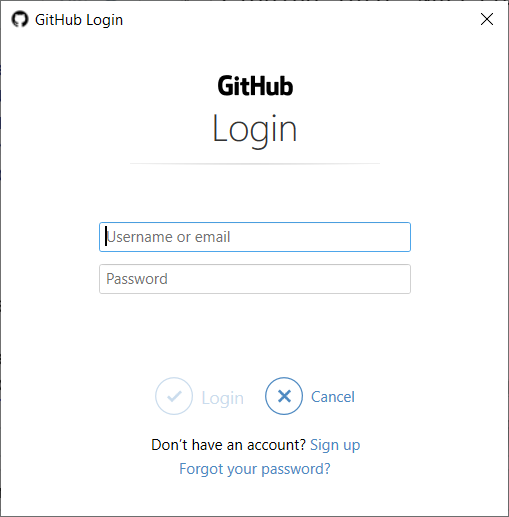
\includegraphics[width=0.8\linewidth]{images/git-PAT} 

}

\caption{Identification HTTPS sur GitHub.}\label{fig:git-PAT}
\end{figure}

\normalsize

Depuis août 2021, GitHub n'accepte plus le mot de passe du compte de l'utilisateur pour cette authentification: le jeton personnel (PAT) créé en section \ref{sec:pat} doit être saisi à sa place.

Si l'authentification SSH est choisie et a été configurée à l'installation de git (section \ref{sec:SSH}), aucune action n'est nécessaire.

\subsection{Pousser les premières modifications}\label{pousser-les-premiuxe8res-modifications}

La manipulation précédente a automatiquement poussé (\emph{Push}) les modifications validées sur GitHub.
Par la suite, il faudra cliquer sur le bouton \enquote{Push} de la fenêtre \emph{Git} pour le faire.

Sur GitHub, les fichiers résultant des modifications enregistrées par git sont maintenant visibles.

Chaque \emph{commit} réalisé localement est compté par git et un message \enquote{Your branch is ahead of \enquote*{origin/master} by \emph{n} commits} affiché dans en haut de la fenêtre \emph{Git} indique qu'il est temps de mettre à jour GitHub en poussant l'ensemble de ces \emph{commits}.
Cliquer sur le bouton \enquote{Push} pour le faire.

A ce stade, le projet doit disposer d'un fichier \texttt{README.md} qui présente son contenu sur GitHub.
Son contenu minimal est un titre et quelques lignes de description:

\begin{verbatim}
# Nom du Projet

Description en quelques lignes.
\end{verbatim}

Il est conseillé d'utiliser des badges\footnote{\url{https://github.com/orangemug/stability-badges}}, à placer juste après le titre, pour déclarer l'état de maturité du projet, par exemple:

\begin{verbatim}
![stability-wip](https://img.shields.io/badge/|>
stability-work_in_progress-lightgrey.svg)
\end{verbatim}

\subsection{Cloner un dépôt de GitHub}\label{cloner-un-duxe9puxf4t-de-github}



\scriptsize

\begin{figure}

{\centering 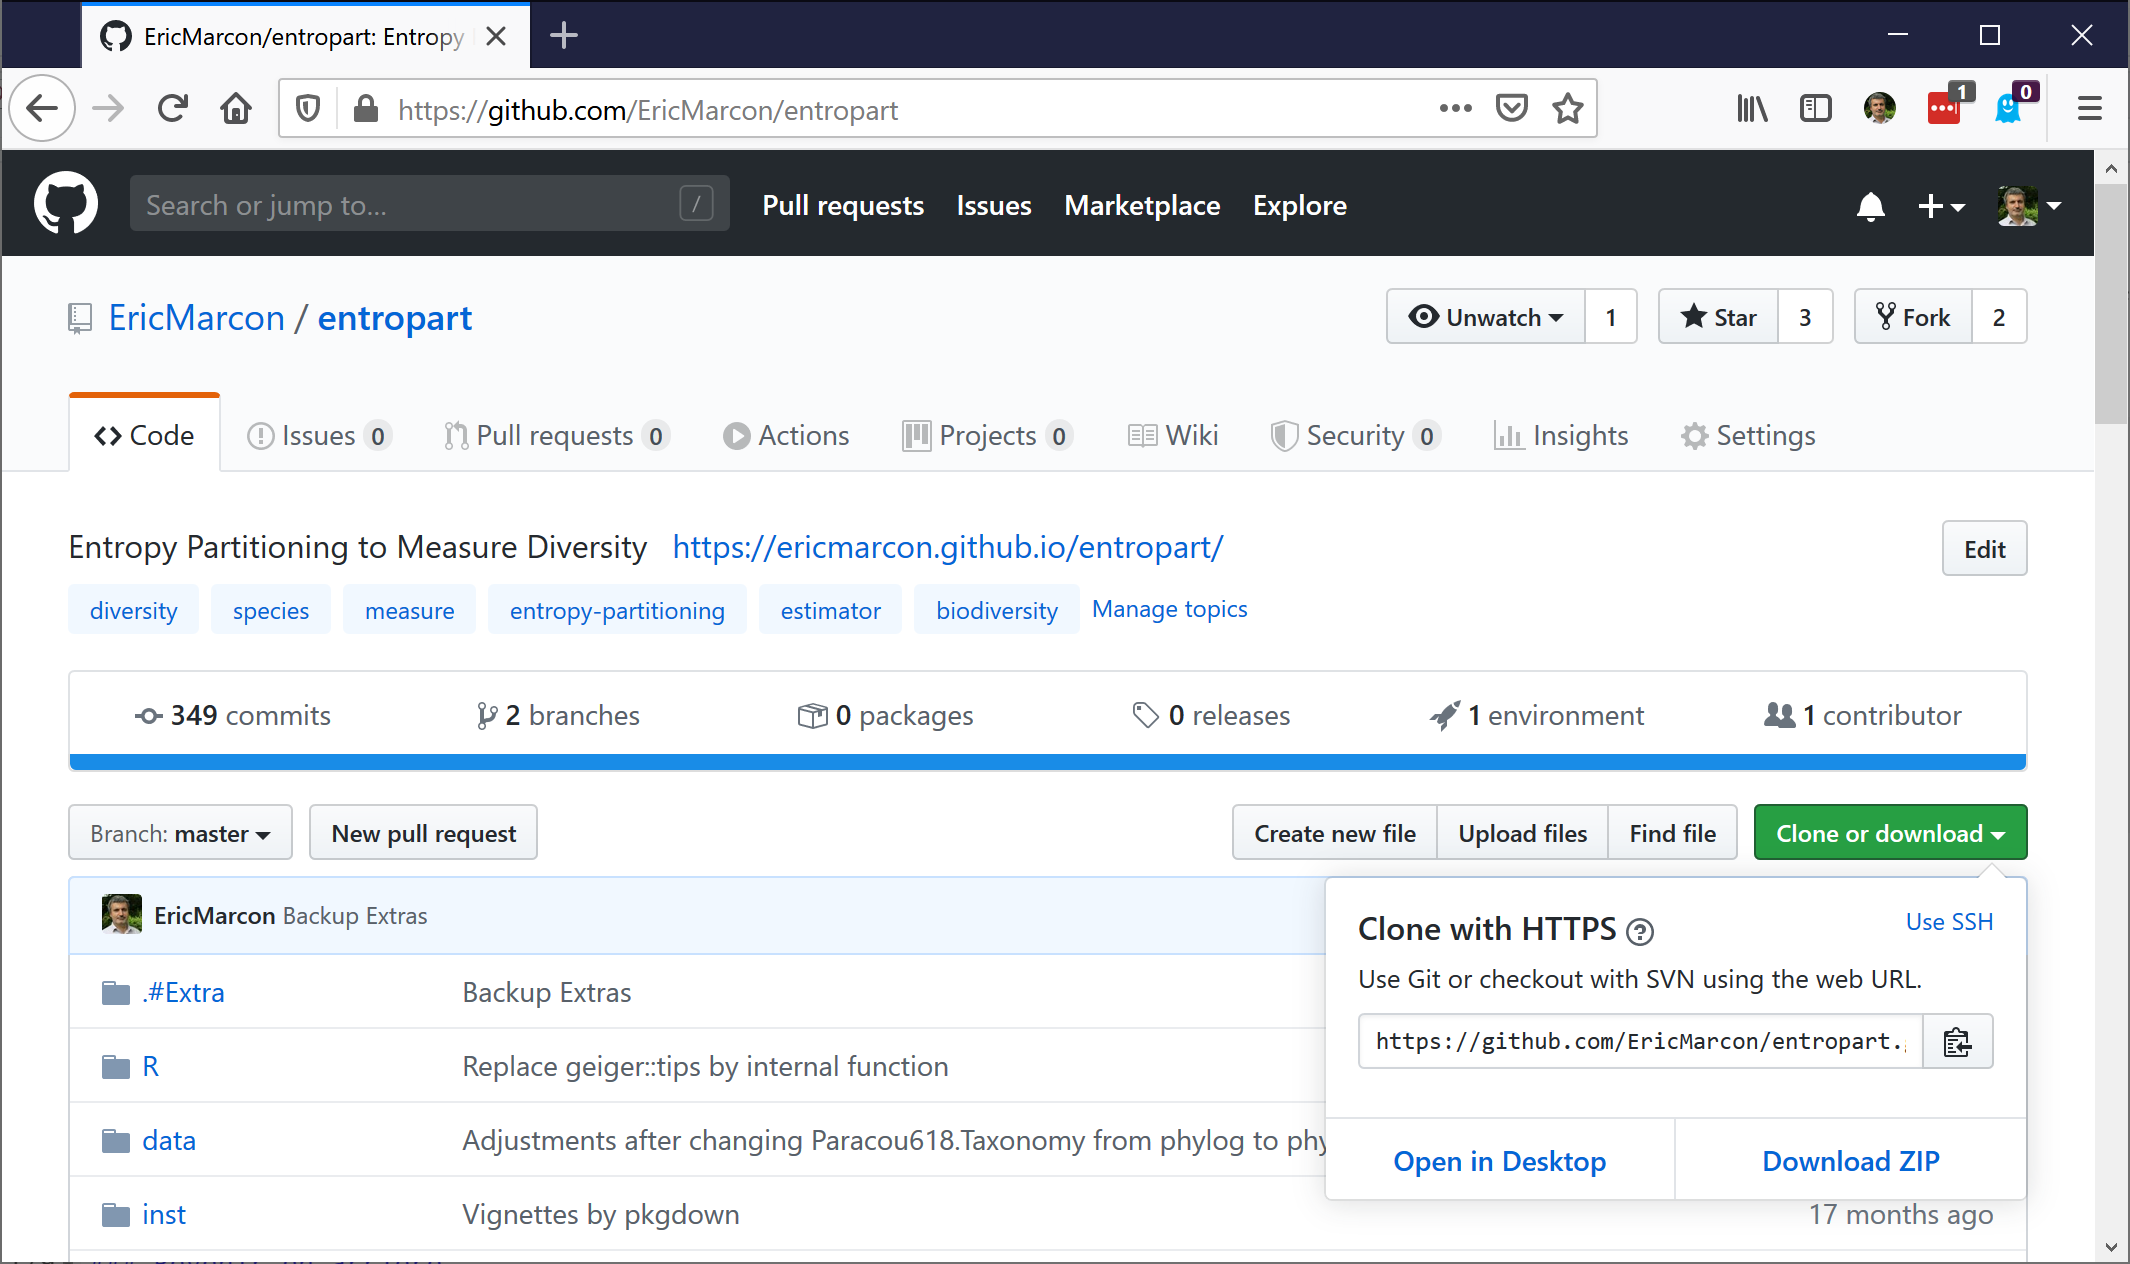
\includegraphics[width=0.8\linewidth]{images/git-Clone} 

}

\caption{Clonage d'un dépôt à partir de \emph{GitHub.}}\label{fig:git-Clone}
\end{figure}

\normalsize

Tout dépôt sur GitHub peut être installé (on dit \emph{cloné}) sur le poste de travail en copiant son adresse qui apparaît en cliquant sur le bouton vert (figure \ref{fig:git-Clone}).

Dans RStudio, créer un nouveau projet et, dans l'assistant, choisir \enquote{Version Control}, \enquote{Git} et coller l'adresse dans le champ \enquote{Repository URL}.
Le nom répertoire à créer pour le projet est déduit automatiquement de l'adresse.
Choisir le répertoire dans lequel celui du projet va être créé et cliquer sur \enquote{Create Project}.
Le projet créé est lié au dépôt distant sur GitHub.

Pour travailler à plusieurs sur le même projet, le propriétaire du projet doit donner l'accès au projet à des collaborateurs (figure \ref{fig:git-Access}), c'est-à-dire d'autres utilisateurs GitHub dans les réglages du dépôt (\emph{Settings}).



\scriptsize

\begin{figure}

{\centering 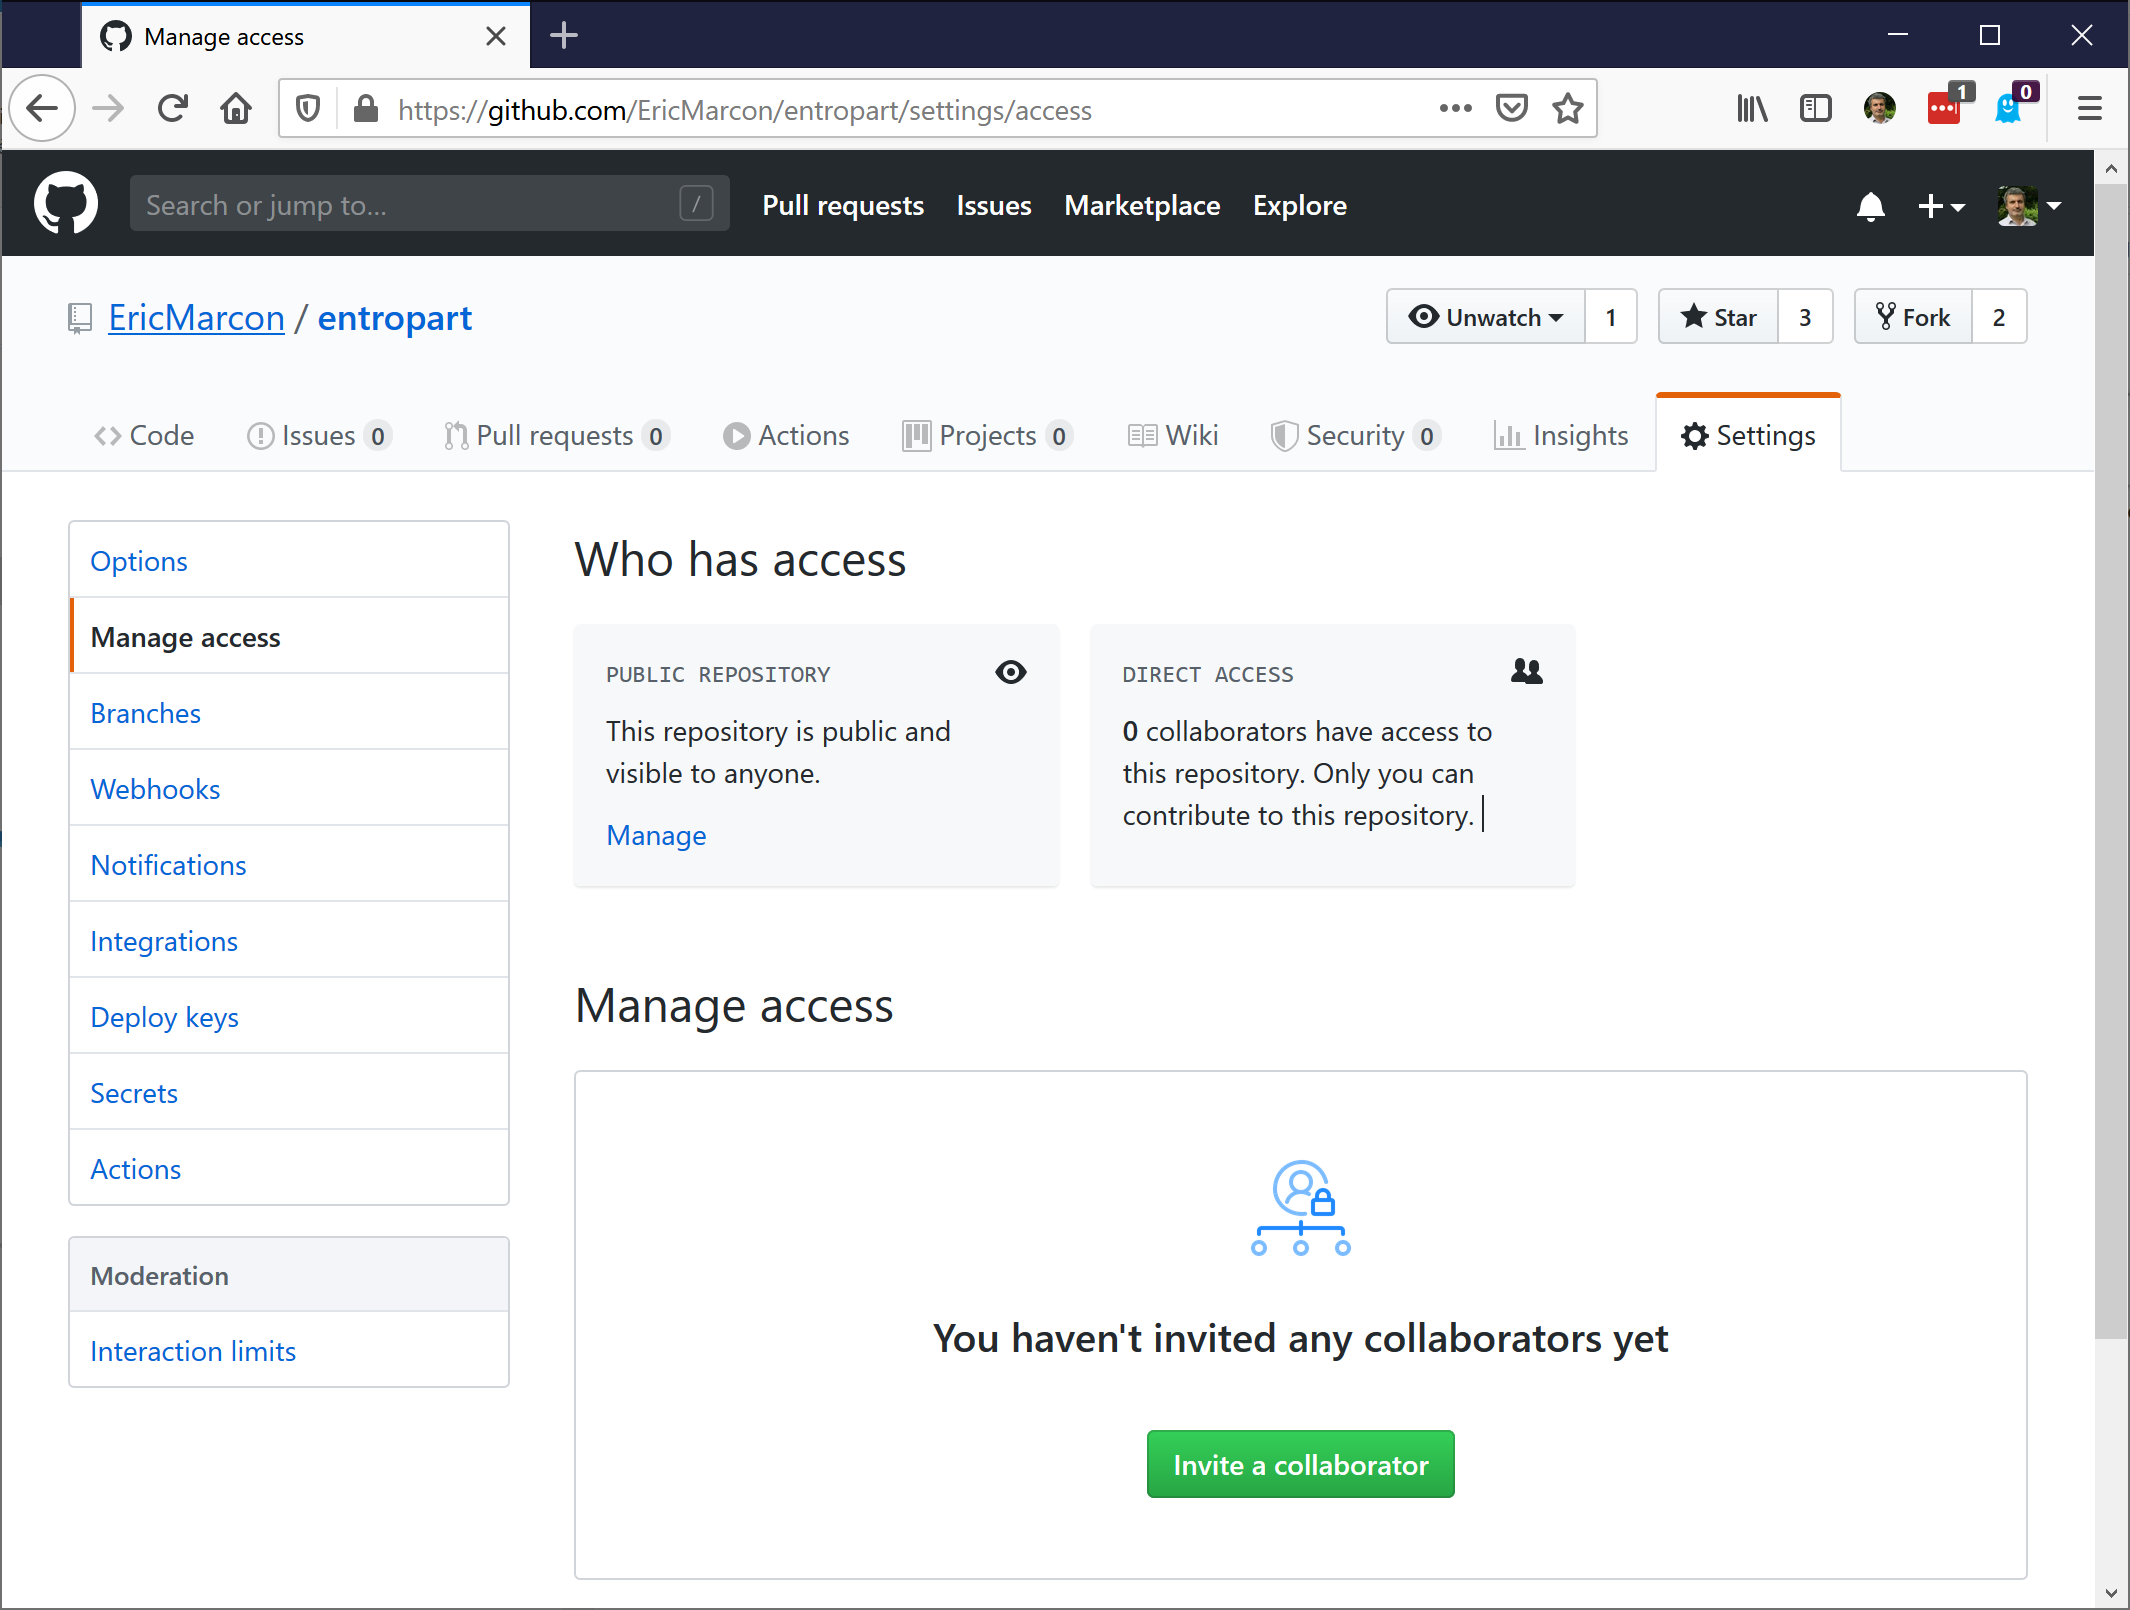
\includegraphics[width=0.8\linewidth]{images/git-Access} 

}

\caption{Attribution des droits d'accès sur GitHub.}\label{fig:git-Access}
\end{figure}

\normalsize

Les collaborateurs sont invités par un message envoyé par \emph{GitHub}.

\section{Usage courant}\label{usage-courant}

\subsection{Tirer, modifier, valider, pousser}\label{tirer-modifier-valider-pousser}

Toute séance de travail sur un projet commence en tirant (Bouton \enquote{Pull}) de la fenêtre \emph{Git} pour intégrer au dépôt local les mises à jour effectuées sur GitHub par d'autres collaborateurs.

Les modifications apportées aux fichiers du projet sont ensuite prises en compte (cocher les cases \emph{Staged}) et validées (\emph{Commit}) avec un message explicatif.
Une bonne pratique consiste à valider les modifications à chaque fois qu'une tâche élémentaire, qui peut être décrite dans le message explicatif, est terminée plutôt que d'effectuer des \emph{commits} regroupant de nombreux changements avec une description vague.

Dès que possible, pousser (\emph{Push}) les mises à jour pour qu'elles soient visibles par les collaborateurs.

\subsection{Régler les conflits}\label{ruxe9gler-les-conflits}

Il n'est pas possible de pousser les modifications validées si un collaborateur a modifié le dépôt distant sur GitHub.
Il faut alors les tirer pour les intégrer au dépôt local avant de pousser les modifications fusionnées.

Un conflit a lieu si un \emph{Pull} importe dans le fichier local une modification qui ne peut pas être fusionnée automatiquement parce qu'une modification contradictoire a eu lieu localement.
Git considère chaque ligne comme un élément indivisible: la modification de la même ligne sur le dépôt distant et le dépôt local génère donc un conflit.

Git insère dans le fichier contenant un conflit les deux versions avec une présentation particulière:

\begin{verbatim}
<<<<<<<<< HEAD # Version importée du conflit
Lignes en conflit, version importée
========= # limite entre les deux versions
Lignes en conflit, version locale
>>>>>>>>> # Fin du conflit
\end{verbatim}

Les lignes de formatage contenant les \texttt{\textless{}\textless{}\textless{}\textless{}}, les \texttt{====} et les \texttt{\textgreater{}\textgreater{}\textgreater{}\textgreater{}} doivent être supprimés et une seule version des lignes problématiques conservée, qui peut être différente des deux versions originales.
La résolution du conflit doit être prise en compte et validée.

Pour limiter les conflits dans un document contenant du texte (typiquement, un document R Markdown), une bonne pratique consiste à traiter chaque phrase comme une ligne, terminée par un retour à la ligne qui ne sera pas visible dans le document mis en forme: un saut de ligne est nécessaire pour séparer les paragraphes.

\subsection{Voir les différences}\label{voir-les-diffuxe9rences}

Dans la fenêtre \emph{Git} de RStudio, le menu contextuel (affiché par un clic droit) \enquote{Diff} peut être utilisé pour afficher les modifications apportées à chaque fichier (figure \ref{fig:git-diff}).



\scriptsize

\begin{figure}

{\centering 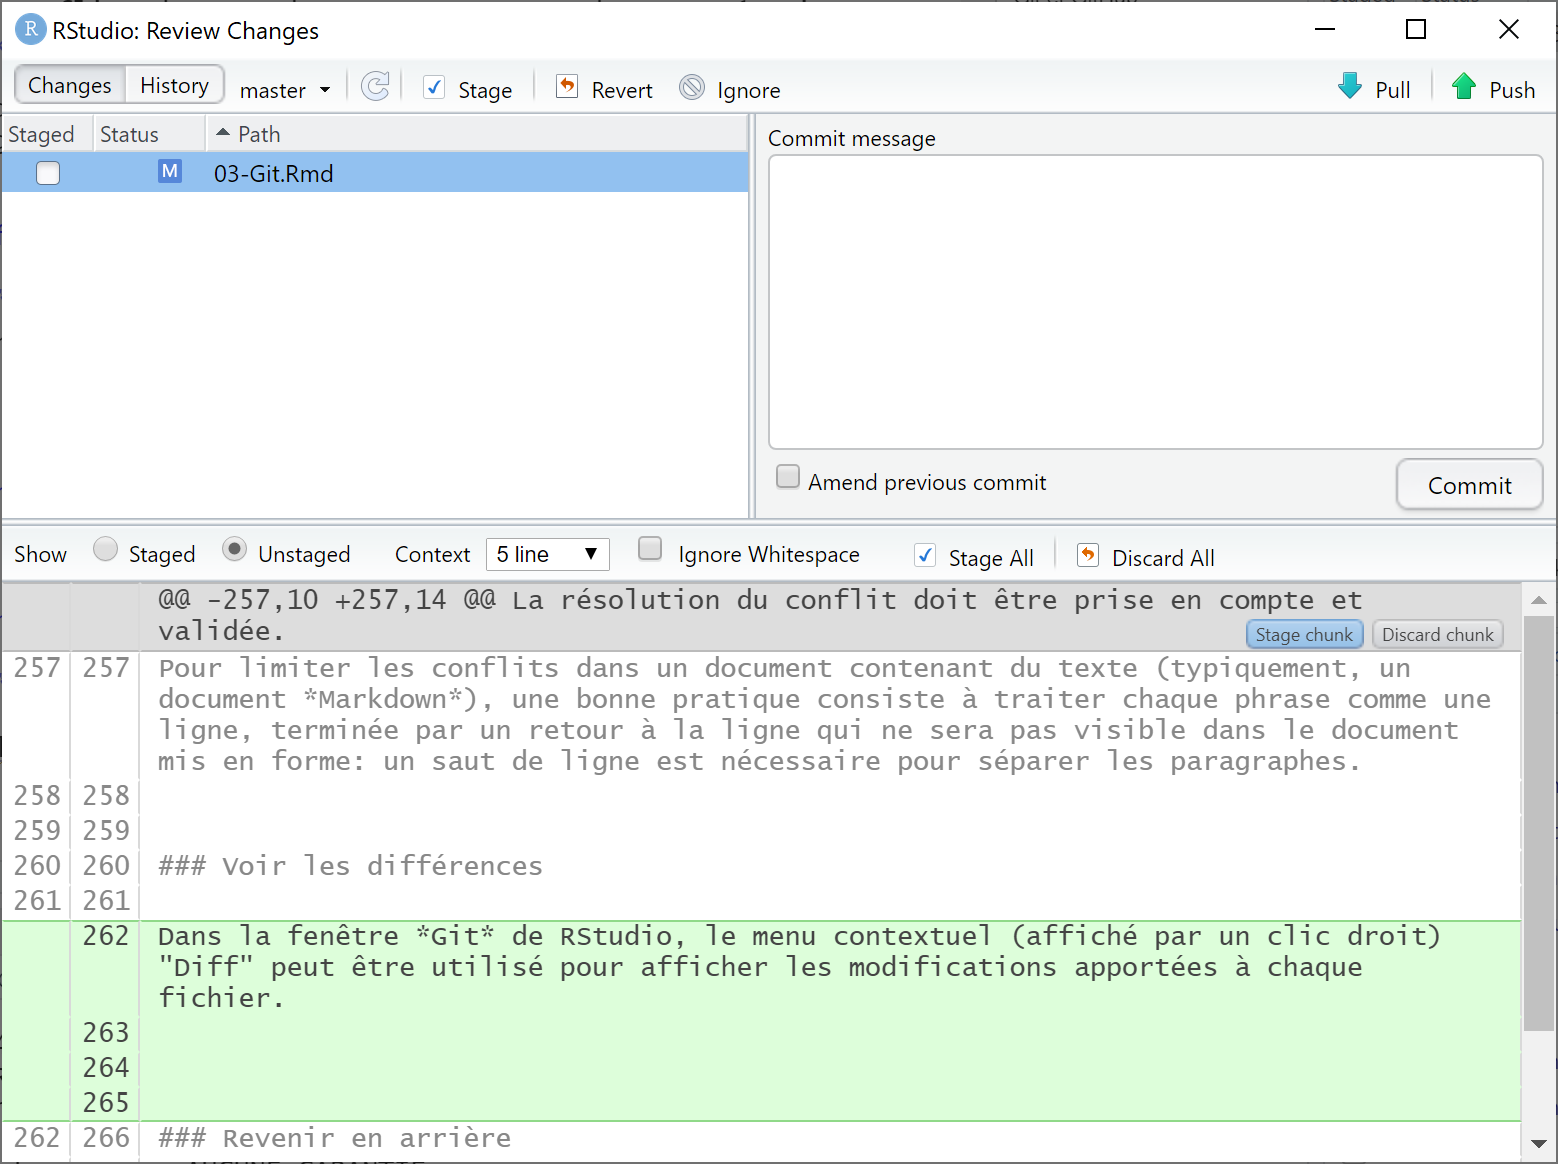
\includegraphics[width=0.8\linewidth]{images/git-diff} 

}

\caption{Différences entre le répertoire de travail et la tête.}\label{fig:git-diff}
\end{figure}

\normalsize

\subsection{Revenir en arrière}\label{revenir-en-arriuxe8re}

Le menu contextuel \enquote{Revert} permet d'annuler toutes les modifications apportées à un fichier (affichées par \emph{Diff}) et de rétablir son contenu validé la dernière fois (son état dans la tête).

Il n'est pas simple de revenir en arrière au-delà de la dernière validation parce que les modifications ont pu être prises en compte par des collaborateurs: leur suppression rendrait le projet incohérent.

\subsection{Voir l'historique}\label{voir-lhistorique}

Le bouton en forme d'horloge de la fenêtre \emph{Git} de RStudio affiche l'historique du projet (figure \ref{fig:git-historique}).



\scriptsize

\begin{figure}

{\centering 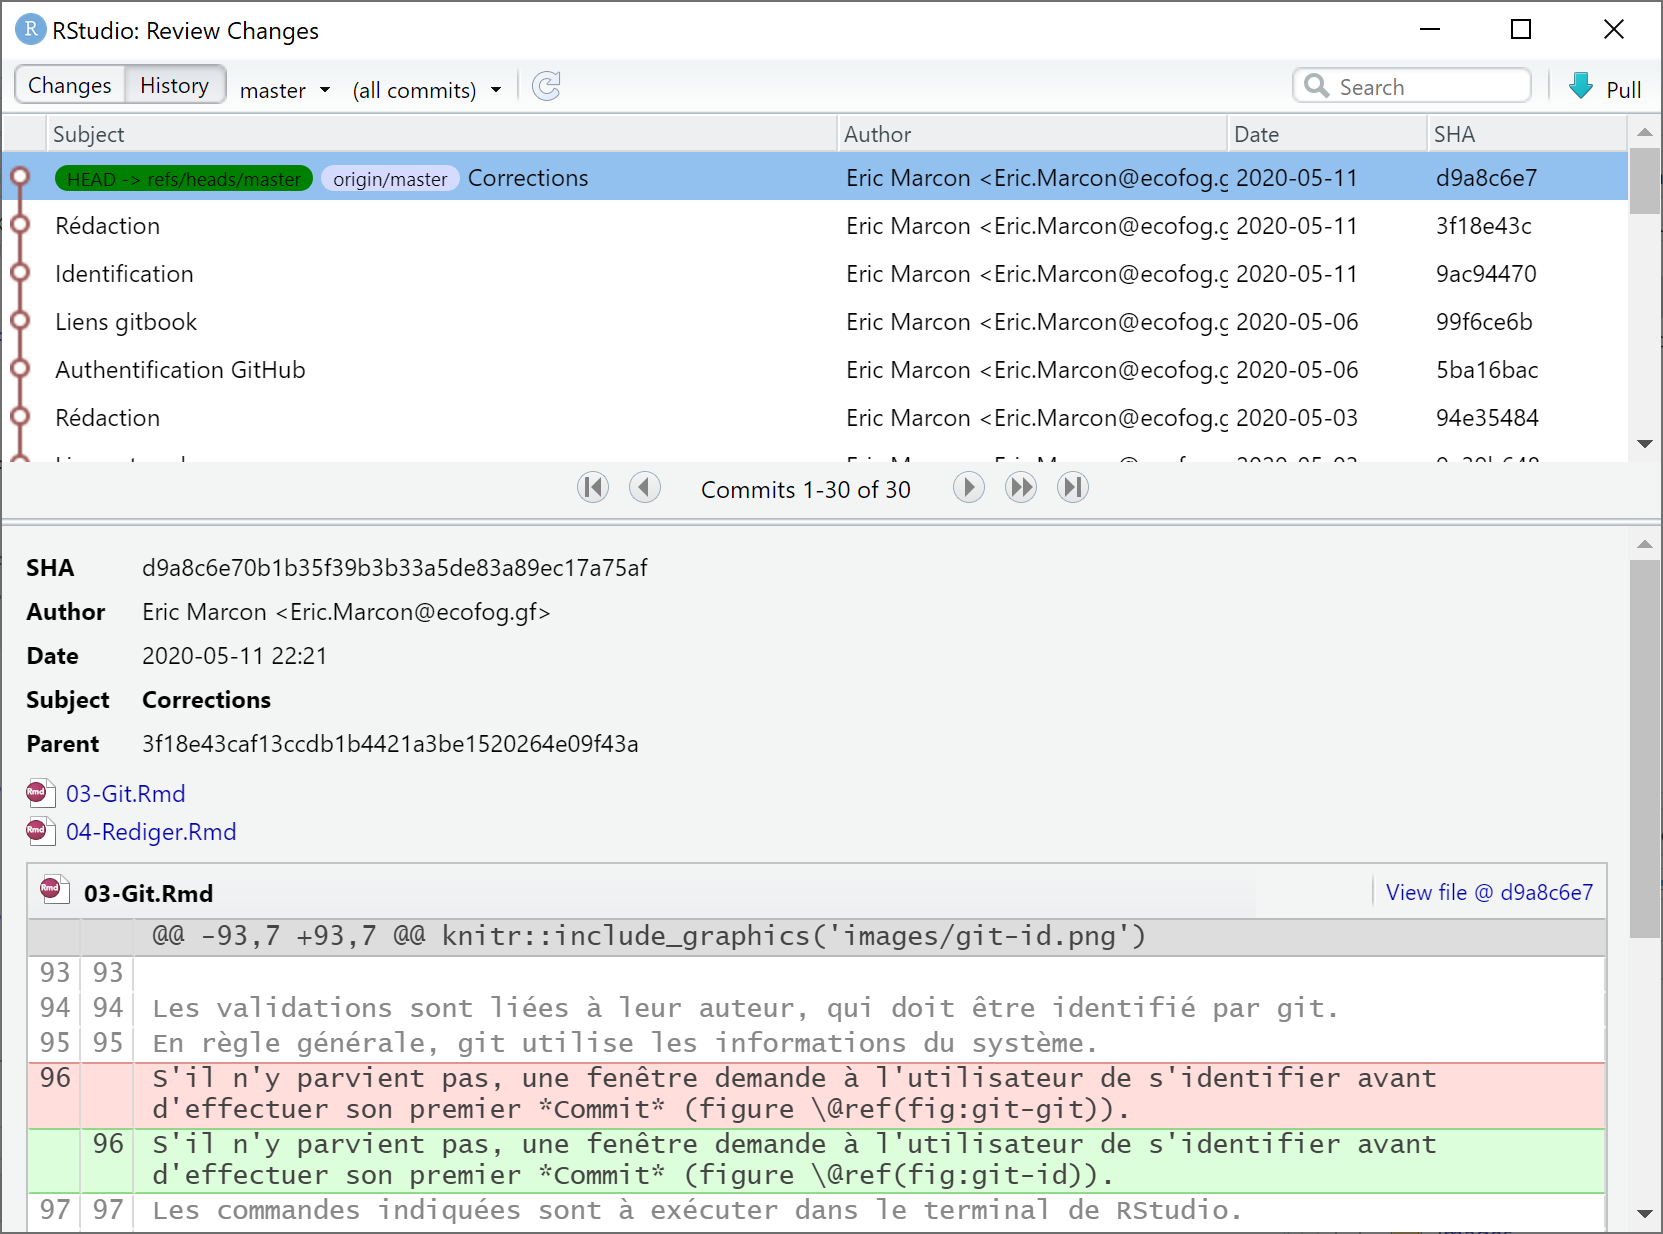
\includegraphics[width=0.8\linewidth]{images/git-historique} 

}

\caption{(ref:git-history)}\label{fig:git-history}
\end{figure}

\normalsize

En haut se trouve la tête, puis toutes les validations (\emph{commits}) qui l'ont constituée.
Pour chaque validation, les différences de chaque fichier peuvent être affichées en cliquant sur le nom du fichier dans la partie basse de la fenêtre.

\section{Branches}\label{sec:branches}

Les branches d'un projet sont des versions différentes mais simultanées.
Un usage typique est le développement d'une nouvelle fonctionnalité.
Si son écriture prend du temps, le projet est perturbé par le chantier en cours: le code peut ne plus fonctionner.
Si le développement s'avère impossible ou inutile, il faut pouvoir l'abandonner sans dommage.
Pour l'isoler pendant sa réalisation et se permettre de le valider ou de l'abandonner à la fin, il faut le placer dans une branche.

La branche principale du projet s'appelle \enquote{master} ou \enquote{main} à partir de novembre 2020\footnote{\url{https://github.com/github/renaming}}.
Elle doit toujours être dans un état stable: c'est elle qui est clonée à partir de GitHub par d'autres utilisateurs éventuels.

Le changement de convention pour le nom de la branche \enquote{master} fait qu'à partir de novembre 2020, les projets créés sur GitHub clonés dans RStudio ont pour branche principale \enquote{main} alors que les projets créés sur RStudio puis liés à GitHub conservent le nom \enquote{master}.

\subsection{Créer une nouvelle branche}\label{cruxe9er-une-nouvelle-branche}

Cliquer sur le bouton violet \enquote{New Branch} dans la fenêtre \emph{git} de RStudio.
Saisir son nom et cliquer sur \enquote{Create}.

La nouvelle branche est maintenant active.

Les commandes git peuvent aussi être exécutées dans le terminal (pour créer la branche et l'activer):

\begin{verbatim}
git branch new_branch
git checkout new_branch
\end{verbatim}

\subsection{Changer de branche}\label{changer-de-branche}

Sélectionner la branche à activer dans la liste des branches locales de la la fenêtre \emph{git}.

Les \emph{commits} s'appliquent à la branche active.
Chaque branche se comporte comme une version différente du projet.

Attention: pour éviter la confusion, sauvegarder les modifications, prendre en compte et valider les changements avant de changer de branche.

\subsection{Pousser la nouvelle branche}\label{pousser-la-nouvelle-branche}

Les premières modifications de la nouvelle branche doivent être poussées en ligne de commande parce que les boutons \enquote{Push} et \enquote{Pull} de la fenêtre \emph{Git} ne fonctionnent pas tant que la branche n'existe pas sur le dépôt distant.

Exécuter, dans le terminal:

\begin{verbatim}
git push -u origin new_branch
\end{verbatim}

\subsection{Comportement du système de fichier}\label{comportement-du-systuxe8me-de-fichier}

A chaque changement de branche, git réécrit les fichiers du projet pour qu'ils reflètent l'état de la branche.
Les changements peuvent être observés hors de RStudio, dans l'explorateur de fichier par exemple.

Les fichiers ignorés par \texttt{.gitignore} ne sont pas modifiés.
Il est donc indispensable que les fichiers \texttt{.gitignore} des différentes branches soit identiques, sinon des fichiers ignorés dans une branche apparaîtront comme ajoutés dans la branche affichée après un changement.

Les branches de développement ont un contenu proche de celui de la branche principale.
Ce n'est pas le cas de branches spécialisées vues plus loin, comme \texttt{gh-pages} (voir section \ref{sec:github-pages}) qui contient le site web de présentation du dépôt.
Il est préférable de ne pas tenter d'afficher ces branches dans RStudio: leur contenu est produit automatiquement et ne doit pas être modifié manuellement.
Si c'est indispensable, il faudra y copier le fichier \texttt{.gitignore} de la branche principale et garder à l'esprit que les fichiers ignorés appartiennent en réalité à une autre branche que celle affichée.

\subsection{\texorpdfstring{Fusionner avec \texttt{merge}}{Fusionner avec merge}}\label{fusionner-avec-merge}

La fusion d'une branche de développement avec la branche principale marque l'atteinte de son objectif: son code va être intégré au projet.
L'interface graphique de RStudio ne prévoit pas les fusions, il faut donc utiliser le terminal: tout d'abord, se placer dans la branche cible (possible avec l'interface graphique):

\begin{verbatim}
git checkout master
\end{verbatim}

Ensuite, fusionner:

\begin{verbatim}
git merge new_branch
\end{verbatim}

Dans la majorité des situations, la fusion sera automatique (\enquote{Fast Forward}).
Il est possible que des conflits apparaissent: utiliser la commande \texttt{git\ status} pour afficher la liste des fichiers concernés, les ouvrir, régler le confit et effectuer un \emph{commit}.

La branche fusionnée n'est pas supprimée: elles peut être utilisée à nouveau pour d'autres développements ou supprimée manuellement avec la commande suivante:

\begin{verbatim}
git branch -d new_branch
\end{verbatim}

\subsection{Fusionner avec une requête de tirage}\label{fusionner-avec-une-requuxeate-de-tirage}

L'autre façon de fusionner est plus formelle mais aussi plus générale: elle permet de fusionner une branche dans un dépôt d'un autre utilisateur pour y contribuer, ou de faire valider sa branche par un autre membre de l'équipe dans un projet collaboratif.

Pour contribuer au projet d'un autre utilisateur de GitHub\footnote{\url{https://git-scm.com/book/fr/v2/GitHub-Contribution-\%C3\%A0-un-projet}}, il faut commencer par en créer un \emph{fork}, c'est-à-dire une copie sous la forme d'un dépôt lié à l'original.
Il sera possible de tirer les modifications de l'original pour rester à jour\footnote{\url{https://ardalis.com/syncing-a-fork-of-a-github-repository-with-upstream/}} (par opposition à une simple copie instantanée possible en téléchargeant un Zip du projet) et, à la fin du développement, de fusionner le \emph{fork} au dépôt original (par opposition à un clone qui ne permettrait pas de contribuer par la suite).

Ensuite, il faut créer une branche de développement comme précédemment, la modifier et finalement demander au propriétaire du dépôt de la fusionner.
Ce processus est décrit en détail dans la documentation de git .

Dans le cadre plus simple d'une branche de son propre projet comme dans le cas d'un \emph{fork}, la branche de développement est prête à être fusionnée.
Elle doit avoir être poussée sur GitHub.
Sur la page GitHub du projet, un bouton \enquote{Create Pull Request} permet de demander la fusion.
Un message décrivant les modifications proposées avec leur argumentaire doit être ajouté.

Le propriétaire du projet (les membres de l'équipe dans le cadre d'un projet collaboratif, ou soi-même si l'équipe se réduit à une personne) est averti de la requête de tirage.
Sur la page du projet original, il est possible de voir le message, la liste des modifications (chronologie des \emph{commits} ou comparaison des fichiers), d'engager un discussion avec l'auteur de la requête\ldots{}
Si la requête n'est pas retenue, elle peut être fermée.
Si elle est validée, le bouton \enquote{Merge Pull Request} permet de fusionner la branche de développement avec la branche \enquote{master} (ou une autre) du projet source.

Les requêtes de tirage sont le seul moyen de contribuer à un dépôt sur lequel on ne dispose pas de droits d'écriture.
C'est aussi le moyen de fusionner une branche de développement dans sont propre projet en en gardant une trace explicite (dans la rubrique \emph{Pull requests} de la page GitHub du projet).
Dans le cadre d'un projet collaboratif, les propositions d'un membre (auteur de la requête) peuvent être validées par un autre (qui accepte la fusion).

\section{Usage avancé}\label{usage-avancuxe9}

\subsection{Commandes de git}\label{commandes-de-git}

Au-delà de l'usage courant permis par l'interface graphique de RStudio, des manipulations avancées des projets sont permises en utilisant git en ligne de commande.
Quelques exemples utiles sont présentés ici.

Un petit guide des commandes est proposé par Roger Dudler\footnote{\url{https://rogerdudler.github.io/git-guide/index.fr.html}}.
Il résume les commandes essentielles, donc intégrées à l'interface graphique de RStudio.
Des liens vers des références plus complètes sont donnés en bas de la page.

\subsection{Taille d'un dépôt}\label{taille-dun-duxe9puxf4t}

Pour connaître l'espace disque occupé par un dépôt, utiliser la commande \texttt{git\ count-objects\ -vH}\footnote{\url{https://git-scm.com/docs/git-count-objects}}.

Les données pour ce document au stade de la rédaction sont présentées à titre d'exemple.

\begin{verbatim}
$ git count-objects -v
count: 200
size: 2.66 MiB
in-pack: 0
packs: 0
size-pack: 0
prune-packable: 0
garbage: 0
size-garbage: 0
\end{verbatim}

La taille totale est sur la ligne \emph{size}.
Les packs sont une méthode utilisée par git pour réduire la taille du dépôt: des fichiers similaires sont stockés sous la forme d'une partie commune et de différences.
La ligne \emph{prune-packable} donne la taille d'objets stockés à la fois sous forme individuelle et dans des packs.
Si leur taille est importante, exécuter \texttt{git\ prune-packed} pour la ramener à zéro.

La ligne \emph{size-garbage} donne la taille des objets qui peuvent être supprimés.
\texttt{git\ gc} les supprime, mais pas seulement: il optimise le stockage.

\begin{verbatim}
$ git gc
Enumerating objects: 194, done.
Counting objects: 100% (194/194), done.
Delta compression using up to 8 threads
Compressing objects: 100% (188/188), done.
Writing objects: 100% (194/194), done.
Total 194 (delta 83), reused 0 (delta 0)

$ git count-objects -vH
count: 1
size: 5.72 KiB
in-pack: 194
packs: 1
size-pack: 4.00 MiB
prune-packable: 0
garbage: 0
size-garbage: 0 bytes
\end{verbatim}

Ici, la majorité des objets du dépôt a été placée dans un pack (mais sa taille est supérieure à celle des objets individuels).

Il est généralement inutile d'effectuer la collecte des déchets manuellement: git gère bien l'organisation de ses dépôts.

GitHub limite la taille des dépôts.
En mai 2020, la limite est de 100 Go.
La taille de tous les dépôts d'un utilisateur authentifié peut être affichée dans les réglages de son compte (\enquote{Personal Settings}, \enquote{Repositories})\footnote{\url{https://github.com/settings/repositories}}.

\subsection{Supprimer un dossier}\label{supprimer-un-dossier}

Toutes les modifications apportées à un dépôt sont stockées dans son historique.
Il peut être utile d'en supprimer dans quelques cas particuliers:

\begin{itemize}
\tightlist
\item
  si un fichier contenant des informations confidentielles a été validé par mégarde.
  La validation de sa suppression ne le retire pas de l'historique, et les informations confidentielles restent visibles en consultant l'historique.
\item
  si des fichiers volumineux ne sont plus nécessaires, par exemple des fichiers PDF produits par R Markdown (chapitre \ref{chap-rediger}), binaires (donc inadaptés à git) et reproductibles à partir du code.
\end{itemize}

Typiquement, le dossier \texttt{docs} est utilisé pour stocker les documents produits à partir de code R Markdown.
Les fichiers HTML et PDF doivent s'y trouver pour constituer les pages GitHub du projet.
Chaque modification du dépôt génère une nouvelle version de ces fichiers dont le volume de l'historique devient rapidement considérable.
Une solution efficace consiste à déléguer la création de ces fichiers à un système d'intégration continue (chapitre \ref{chap-ci}) et à retirer le dossier \texttt{docs} de la branche principale (\emph{master}) du dépôt.
Il faut alors supprimer tout son historique pour récupérer la place qu'il occupe, qui peut être l'essentiel de la taille du dépôt.

Les commandes de suppression complète d'un dossier d'un dépôt son présentées ici\footnote{\url{https://stackoverflow.com/questions/10067848/remove-folder-and-its-contents-from-git-githubs-history}}.
Le dépôt doit être propre, c'est-à-dire sans modifications non validées, et les versions distantes et locales synchronisées.

Les trois commandes suivantes suppriment complètement le dossier \texttt{docs} de l'historique du dépôt git:

\begin{verbatim}
git filter-branch --tree-filter "rm -rf docs" |>
    --prune-empty HEAD
git for-each-ref --format="%(refname)" refs/original/ |>
    | xargs -n 1 git update-ref -d
\end{verbatim}

Le dossier n'est pas supprimé du répertoire de travail.
Il doit donc être ajouté au fichier \texttt{.gitignore} pour ne plus être suivi.
La modification de \texttt{.gitignore} doit être validée.
Ces opérations peuvent être réalisées avec l'interface de RStudio ou en ligne de commande:

\begin{verbatim}
echo docs/ >> .gitignore
git add .gitignore
git commit -m 'Removing docs folder from git history'
\end{verbatim}

Le nettoyage du dépôt est nécessaire pour supprimer physiquement les données retirées:

\begin{verbatim}
git gc
\end{verbatim}

Enfin, le dépôt doit être poussé.
L'option \texttt{-\/-force} implique le remplacement du contenu du dépôt distant par celui du dépôt local: toutes les modifications faites par des collaborateurs sont effacées, c'est pourquoi cette opération de nettoyage implique l'arrêt complet du projet pendant qu'elle a lieu.

\begin{verbatim}
git push origin master --force
\end{verbatim}

Ce code peut être utilisé pour supprimer totalement n'importe quel fichier ou dossier d'un dépôt en remplaçant simplement \texttt{docs} dans la commande \texttt{git\ filter-branch} initiale.
La réduction de la taille du dépôt peut être suivie en utilisant \texttt{git\ count-objects\ -vH} avant l'opération, avant \texttt{git\ gc} (la taille du dépôt reste stable mais a été déplacée vers \emph{garbage}) et à la fin (la taille du dépôt est sensiblement réduite).

\subsection{Revenir en arrière}\label{revenir-en-arriuxe8re-1}

Il est possible de restaurer un dépôt dans un état précédent en plaçant sa tête (figure \ref{fig:git-Trees}) au niveau d'un ancien \emph{commit}.
Toutes les modifications ultérieures sont alors détruites.
Cette opération ne doit pas être réalisée sur un dépôt partagé: les autres utilisateurs ne pourraient plus pousser leurs modifications.

Afficher l'historique du dépôt et rechercher l'identifiant (SHA) du dernier \emph{commit} à conserver.
Dans le terminal de RStudio, exécuter:

\begin{verbatim}
git reset --hard <SHA>
git push -f
\end{verbatim}

Tout l'historique du dépôt après le point de restauration choisi est perdu.

Une méthode moins radicale et utilisable sur un dépôt partagé consiste à exécuter un \emph{commit} qui annule les modifications d'un autre mais ne détruit aucune donnée de l'historique.
Cette opération n'annule qu'un seul \emph{commit} à la fois et doit donc être répétée pour en annuler plusieurs, en commençant par le plus récent.
Dans le terminal de RStudio, exécuter:

\begin{verbatim}
git revert <SHA>
\end{verbatim}

Pour annuler le dernier \emph{commit}, exécuter:

\begin{verbatim}
git revert HEAD
\end{verbatim}

Utiliser \texttt{HEAD} évite simplement de rechercher l'identifiant correspondant.

\section{Données confidentielles dans un dépôt public}\label{sec:confidentiel}

Un dépôt public sur GitHub pose problème quand des données utilisées dans le projet ne le sont pas.

Une solution peu satisfaisante consiste à ne pas inclure les données au projet, ce qui le rend non reproductible.
Une meilleure solution est de les crypter, en permettant à certains utilisateurs de les décrypter.
C'est l'objet du package \textbf{secret}.

Un coffre-fort (dossier \texttt{vault}) est créé dans le projet.
Il contient une liste d'utilisateurs autorisés: chacun d'entre eux doit disposer d'une paire de clés de cryptage, une clé publique incluse dans le coffre-fort et une clé privée, gardée secrète.
Les données sont cryptées avec toutes les clés publiques disponibles (et donc dupliquées).
Les utilisateurs utilisent ensuite chacun sa clé privée pour le décryptage.

Pour ne pas multiplier les copies des données, le propriétaire du dépôt a intérêt à créer un utilisateur générique pour le projet, dont il communiquera la clé privée hors de GitHub.
Le coffre contiendra les clés du propriétaire du projet et de l'utilisateur générique seulement.
En cas de compromission de la clé privée de l'utilisateur générique, il suffira de le retirer du coffre-fort et d'en créer un nouveau.

\subsection{Génération d'une paire de clés pour le propriétaire du projet}\label{guxe9nuxe9ration-dune-paire-de-cluxe9s-pour-le-propriuxe9taire-du-projet}

Les clés sont générées par le logiciel \emph{ssh}, installé avec \emph{git} ou par défaut sous Linux.

La procédure est identique à celle de la section \ref{sec:SSH}, mais la clé utilisée doit être au format RSA (pris en charge par le package \textbf{secret}, contrairement au format ed25519, plus sûr, utilisé pour l'authenfication sur GitHub).

Exécuter la commande suivante dans le terminal de RStudio pour créer une clé RSA:

\begin{verbatim}
ssh-keygen -t rsa -b 4096 -C "user.email"
\end{verbatim}

Stocker la clé publique sur GitHub dans \enquote{Settings \textgreater{} SSH and GPG Keys}.
Repérer la position de la clé: si une clé d'authentification a déjà été enregistrée pour deux postes de travail par exemple, la clé RSA sera la troisième.

\subsection{Génération d'une paire de clés pour le projet}\label{guxe9nuxe9ration-dune-paire-de-cluxe9s-pour-le-projet}

Générer une clé au format RSA dans le terminal de RStudio:

\begin{verbatim}
ssh-keygen -t rsa -b 4096" 
\end{verbatim}

\begin{itemize}
\tightlist
\item
  Entrer le nom de la clé: \texttt{\textless{}RepoID\textgreater{}.rsa}.
\item
  Ne pas saisir de phrase de validation (mot de passe) pour permettre l'utilisation de la clé sans interaction.
\end{itemize}

La clé privée \texttt{\textless{}RepoID\textgreater{}.rsa} ne doit être diffusée qu'aux ayant-droits du projet.
Il faut donc ajouter la ligne \texttt{*.rsa} au fichier \texttt{.gitignore} du projet pour ne pas pousser la clé sur GitHub.

Pour permettre l'intégration continue du projet (chapitre \ref{chap-ci}), la clé privée doit être stockée comme un secret du dépôt GitHub contenant le projet.
Appliquer la procédure de la section \ref{sec:secrets-ci} pour créer un secret nommé \enquote{RSA} et coller le contenu du fichier \texttt{\textless{}RepoID\textgreater{}.rsa} dans le champ \enquote{Value} du formulaire.

L'utilisation du secret est décrite dans la section \ref{sec:confidentielCI}.

\subsection{Création d'un coffre-fort}\label{cruxe9ation-dun-coffre-fort}

Exécuter:

\scriptsize

\begin{Shaded}
\begin{Highlighting}[]
\FunctionTok{library}\NormalTok{(}\StringTok{"secret"}\NormalTok{)}
\NormalTok{vault }\OtherTok{\textless{}{-}} \StringTok{"vault"}
\FunctionTok{create\_vault}\NormalTok{(vault)}
\end{Highlighting}
\end{Shaded}

\normalsize

\subsection{Ajout des utilisateurs}\label{ajout-des-utilisateurs}

Le propriétaire du projet est ajouté à partir de sa clé publique stockée sur GitHub, qui est la troisième dans notre exemple.

\scriptsize

\begin{Shaded}
\begin{Highlighting}[]
\CommentTok{\# Identifiant GitHub du propriétaire du projet}
\NormalTok{github\_user }\OtherTok{\textless{}{-}} \StringTok{"EricMarcon"}
\CommentTok{\# Lecture et stockage de la clé, i est le numéro de la clé}
\FunctionTok{add\_github\_user}\NormalTok{(github\_user, }\AttributeTok{vault =}\NormalTok{ vault, }\AttributeTok{i =} \DecValTok{3}\NormalTok{)}
\end{Highlighting}
\end{Shaded}

\normalsize

La clé de l'utilisateur générique du projet est ajoutée par:

\scriptsize

\begin{Shaded}
\begin{Highlighting}[]
\FunctionTok{library}\NormalTok{(}\StringTok{"openssl"}\NormalTok{)}
\NormalTok{project\_id }\OtherTok{\textless{}{-}} \StringTok{"NomDuProjet"}
\CommentTok{\# Lecture de la clé}
\NormalTok{rsa\_project }\OtherTok{\textless{}{-}} \FunctionTok{read\_pubkey}\NormalTok{(}\FunctionTok{paste0}\NormalTok{(project\_id, }\StringTok{".rsa.pub"}\NormalTok{))}
\CommentTok{\# Ajout au coffre{-}fort}
\FunctionTok{add\_user}\NormalTok{(project\_id, }\AttributeTok{public\_key =}\NormalTok{ rsa\_project, }\AttributeTok{vault =}\NormalTok{ vault)}
\end{Highlighting}
\end{Shaded}

\normalsize

\subsection{Stockage des données}\label{stockage-des-donnuxe9es}

Les données, stockées dans des variables de R, sont stockées une à une par la fonction \texttt{add\_secret()}.
Dans l'exemple suivant, la variable s'appelle \texttt{X} et vaut 1.

\scriptsize

\begin{Shaded}
\begin{Highlighting}[]
\NormalTok{X }\OtherTok{\textless{}{-}} \DecValTok{1}
\FunctionTok{add\_secret}\NormalTok{(}
  \CommentTok{\# Nom de la donnée}
  \StringTok{"X"}\NormalTok{, }
  \CommentTok{\# Valeur}
  \AttributeTok{value =}\NormalTok{ X, }
  \CommentTok{\# Utilisateurs autorisés: propriétaire et générique}
  \AttributeTok{users =} \FunctionTok{c}\NormalTok{(}\FunctionTok{paste0}\NormalTok{(}\StringTok{"github{-}"}\NormalTok{, github\_user), project\_id), }
  \CommentTok{\# Coffre{-}fort}
  \AttributeTok{vault =}\NormalTok{ vault}
\NormalTok{)}
\end{Highlighting}
\end{Shaded}

\normalsize

Le contenu du coffre-fort peut être vérifié:

\scriptsize

\begin{Shaded}
\begin{Highlighting}[]
\CommentTok{\# Liste des données du coffre}
\FunctionTok{list\_secrets}\NormalTok{(}\AttributeTok{vault =}\NormalTok{ vault)}
\end{Highlighting}
\end{Shaded}

\begin{verbatim}
##   secret        email
## 1      X github-E....
\end{verbatim}

\begin{Shaded}
\begin{Highlighting}[]
\CommentTok{\# Liste des propriétaire de la donnée "X"}
\FunctionTok{list\_owners}\NormalTok{(}\StringTok{"X"}\NormalTok{, }\AttributeTok{vault =}\NormalTok{ vault)}
\end{Highlighting}
\end{Shaded}

\begin{verbatim}
## [1] "github-EricMarcon" "NomDuProjet"
\end{verbatim}

\normalsize

Les données seront lues dans le code du projet par la commande \texttt{get\_secret()}.
La clé privée de l'utilisateur générique du projet, communiquée par un moyen sécurisé aux ayant-droits, doit se trouver dans le dossier du projet.

\scriptsize

\begin{Shaded}
\begin{Highlighting}[]
\CommentTok{\# Sélection de la clé privée}
\FunctionTok{Sys.setenv}\NormalTok{(}\AttributeTok{USER\_KEY =}\NormalTok{ usethis}\SpecialCharTok{::}\FunctionTok{proj\_path}\NormalTok{(}\FunctionTok{paste0}\NormalTok{(project\_id, }\StringTok{".rsa"}\NormalTok{)))}
\CommentTok{\# Lecture de la donnée "X"}
\FunctionTok{get\_secret}\NormalTok{(}\StringTok{"X"}\NormalTok{, }\AttributeTok{vault =}\NormalTok{ vault)}
\end{Highlighting}
\end{Shaded}

\begin{verbatim}
## [1] 1
\end{verbatim}

\normalsize

La clé peut être vérifiée:

\scriptsize

\begin{Shaded}
\begin{Highlighting}[]
\FunctionTok{local\_key}\NormalTok{()}
\end{Highlighting}
\end{Shaded}

\begin{verbatim}
## [4096-bit rsa private key]
## md5: e81dcb0745a755286c2dc1fc4c6ad117
## sha256: cca11ef82e17c3b77b699e7f3c23e083e8f0f79cb70be8274799f076c44b0c2d
\end{verbatim}

\normalsize

\section{Pages GitHub}\label{sec:github-pages}

Tout projet sur GitHub doit avoir contenir un fichier \texttt{README.md} pour le présenter.
Ce fichier est écrit au format Markdown.

Le fichier peut être placé dans le dossier \texttt{docs} pour fournir à fois la page d'accueil du dépôt et de son site web.
Le package \textbf{memoiR} fournit des commandes permettant d'automatiser ces tâches dans les projets de documents.
Un dépôt contenant un article écrit en R Markdown (voir section \ref{sec:memo}) est utilisé comme exemple\footnote{\url{https://github.com/EricMarcon/Krigeage}}.

Son fichier \texttt{README.md} existe aux deux emplacements: il est écrit par le développeur à la racine du projet et dupliqué dans \texttt{docs}.

\subsection{Activation}\label{activation}

Pour activer les pages GitHub, il faut ouvrir les propriétés du dépôt (\emph{Settings}) et modifier la rubrique \enquote{GitHub Pages} (dans \enquote{Options}).
Sélectionner la branche du projet et le dossier contenant les pages web, ici: \texttt{master} et \texttt{/docs}.
En option, le choix d'un thème personnalise l'apparence des pages.

Le site web est accessible à une adresse\footnote{\url{https://EricMarcon.github.io/Krigeage/}} du domaine \emph{github.io}.

Le fichier \texttt{README.md} affiché en page d'accueil a un aspect très différent mais le même contenu que celui affiché avec le code sur la page du dépôt dans GitHub.

L'intérêt des pages GitHub est de permettre un accès simple aux documents formatés quand le dépôt contient une production écrite et ou à la documentation des packages R.
Ces contenus seront présentés dans le chapitre suivant.

Un site web principal est proposé avec chaque compte GitHub, à l'adresse \url{https://GitHubID.github.io}\footnote{Exemple: \url{https://EricMarcon.github.io/Krigeage/}}.
Il sera utilisé pour héberger un site web personnel produit par \textbf{blogdown}.

\subsection{Badges}\label{badges}

Les badges sont de petites images, éventuellement mises à jour dynamiquement, qui renseignent rapidement sur le statut d'un projet.
Ils doivent être placés immédiatement après le titre du fichier \texttt{README.md}.

Une bonne pratique consiste à indiquer l'avancement dans le cycle de vie du projet.
Les badges correspondants sont listés sur le site du Tidyverse\footnote{\url{https://www.tidyverse.org/lifecycle/}}.

Leur code Markdown est le suivant:

\begin{verbatim}
![stability-wip]
(https://img.shields.io/badge/lifecycle-maturing-blue.svg)
\end{verbatim}

Le package \textbf{usethis} simplifie leur création en plaçant le code nécessaire dans le presse-papier.
Il suffit ensuite de le coller dans le fichier.

\scriptsize

\begin{Shaded}
\begin{Highlighting}[]
\NormalTok{usethis}\SpecialCharTok{::}\FunctionTok{use\_lifecycle\_badge}\NormalTok{(}\StringTok{"maturing"}\NormalTok{)}
\end{Highlighting}
\end{Shaded}

\normalsize

\chapter{Rédiger}\label{chap-rediger}

\toc{1}

R et RStudio permettent de rédiger efficacement des documents de tous formats, du simple bloc-note à la thèse, en passant par des diaporamas.
Les outils pour le faire sont l'objet de ce chapitre, complété par la production de sites web (y compris un site personnel).

Deux procédés de production de documents sont disponibles:

\begin{itemize}
\tightlist
\item
  \emph{R Markdown} avec les packages \textbf{knitR} et \textbf{bookdown}.
  C'est ma méthode classique, présentée ici en détail.
\item
  \emph{Quarto}, conçu pour être utilisé avec d'autres langages que R et dans d'autres environnements de travail que RStudio.
  Quarto est en développement actif mais ne permet pas encore de produire des documents avec la même qualité que \emph{R Markdown}: par exemple, la ponctuation des documents en français n'est pas gérée correctement en PDF\footnote{\url{https://github.com/jgm/pandoc/issues/8283/}}, les tableaux ne peuvent pas inclure d'équations\footnote{\url{https://github.com/quarto-dev/quarto-cli/issues/555}} et la largeur des figures est incohérente dans les documents PDF formatés avec plusieurs colonnes\footnote{\url{https://github.com/quarto-dev/quarto-cli/issues/855}}.
  L'usage de Quarto est bien documenté sur son site\footnote{\url{https://quarto.org/}} et n'est pas présenté ici.
\end{itemize}

\section{Bloc-note Markdown (R Notebook)}\label{bloc-note-markdown-r-notebook}

Dans un fichier \texttt{.R}, le code doit toujours être commenté pour faciliter sa lecture.
Quand l'explication du code nécessite plusieurs lignes de commentaire par ligne ou bloc de code, il est temps d'inverser la logique et de placer le code dans un texte.

Le concept de programmation lettrée (\emph{literate programming}) a été développé par \textcite{Knuth1984}.
Il s'agit de décrire les objectifs et les méthodes par du texte, dans lequel le code s'intègre.

L'outil le plus simple est le bloc-note Markdown (Menu \enquote{File \textgreater{} New File \textgreater{} R Notebook}).
Le modèle de document contient son mode d'emploi.

Le langage qui permet de formater le texte est Markdown\footnote{\url{https://fr.wikipedia.org/wiki/Markdown}}, un langage de balisage simple à utiliser:

\begin{itemize}
\tightlist
\item
  Les paragraphes sont séparés par des sauts de ligne;
\item
  Le document est structuré par des titres: leur ligne commence par un nombre de \texttt{\#} correspondant à leur niveau;
\item
  Les formats de caractères sont limités à l'essentiel: italique ou gras (texte entouré par une ou deux \texttt{*});
\item
  D'autres codes simples permettent tous les formatages utiles.
\end{itemize}

Ce langage est le pivot du logiciel pandoc\footnote{\url{https://fr.wikipedia.org/wiki/Pandoc}}, dédié à la conversion de documents de formats différents.

Le package \textbf{rmarkdown} \autocite{Xie2015} fait le lien entre R et Markdown, en s'appuyant sur l'interface de RStudio qui n'est pas indispensable mais simplifie énormément son utilisation.
Le dialecte de Markdown utilisé par le package est appelé \emph{R Markdown}.
Sa syntaxe est résumée dans une antisèche\footnote{\url{https://rstudio.com/wp-content/uploads/2015/02/rmarkdown-cheatsheet.pdf}}.
Sa documentation complète est en ligne \autocite{Xie2018}.

Les équations sont écrites au format LaTeX\footnote{\url{https://fr.wikibooks.org/wiki/LaTeX/\%C3\%89crire_des_math\%C3\%A9matiques}}.

L'organisation la plus simple d'un document \emph{R Markdown} est visible dans le modèle de bloc-note.
Il commence par un en-tête au format YAML\footnote{\url{https://fr.wikipedia.org/wiki/YAML}}:

\begin{verbatim}
---
title: "R Notebook"
output: html_notebook
---
\end{verbatim}

La première entrée est le titre, la seconde le format de sortie: plus précisément le nom de la fonction chargée de traiter le document.

Le document contient du texte formaté en Markdown et des bouts de code (\emph{code chunks}) entourés par trois accents graves (la syntaxe markdown d'un bloc de code) et une description du langage, ici \texttt{r}.
Ces bouts de code sont traités par \textbf{knitr} qui transforme le résultat de l'exécution du code R en Markdown et l'intègre au texte du document.

Traiter un document R Markdown s'appelle le \emph{tricoter} (\emph{knit}).
La chaîne de production est la suivante:

\begin{itemize}
\tightlist
\item
  \textbf{knitr} traite les bouts de code: calculs, production de figures;
\item
  \textbf{rmarkdown} intègre la production des bouts de code et texte pour produire un fichier Markdown standard;
\item
  pandoc (installé avec RStudio) convertit ce fichier au format HTML, LaTeX ou Word;
\item
  LaTeX produit un fichier PDF quand ce format est demandé.
\end{itemize}

RStudio permet de lancer le tricot par des boutons plutôt que par des commandes: dans la fenêtre source (celle du haut à gauche), un bouton \enquote{Knit} accompagne les documents R Markdown.
Pour les bloc-notes R Markdown, il est remplacé par un bouton \enquote{Preview} avec les mêmes fonctions.
Il peut être déroulé pour choisir le format de sortie: HTML, Word, PDF (en passant par LaTeX) et, pour les bloc-notes, une commande \enquote{Preview} qui affiche le document en HTML sans exécuter les bouts de code pour gagner du temps.
Dès le premier tricot au format Word ou HTML, on remarquera que le bouton \enquote{Preview} disparaît.

Au final, l'utilisation de R Markdown combine plusieurs avantages:

\begin{itemize}
\tightlist
\item
  La simplicité de la rédaction: le texte brut est plus facile à lire et à formater qu'en LaTeX par exemple;
\item
  L'automatisation de la production: le formatage et la mise en page sont entièrement automatiques;
\item
  La reproductibilité: chaque document peut être autosuffisant accompagné de ses données. Relancer le tricotage régénère entièrement le document, y compris les calculs nécessaires et la production des figures.
\end{itemize}

Elle a aussi quelques inconvénients:

\begin{itemize}
\tightlist
\item
  Le formatage dépend de modèles, et developper de nouveaux modèles n'est pas simple;
\item
  Les erreurs de tricot sont parfois difficiles à corriger, notamment quand elles interviennent à l'étape de la compilation LaTeX;
\item
  La reproductibilité consomme du temps de calcul. Pour limiter ce problème, un système de cache permet de ne pas réévaluer tous les bouts de code R à chaque modification du texte. La production de gros documents peut aussi être déléguée à un système d'intégration continue (chapitre \ref{chap-ci}).
\end{itemize}

\section{Modèles R Markdown}\label{moduxe8les-r-markdown}

Des modèles de document plus élaborés que le bloc-note sont fournis par des packages, dont \textbf{rmarkdown}.
Ils sont accessibles par le menu \enquote{File \textgreater{} New File \textgreater{} R Markdown\ldots{}} (figure \ref{fig:e-rmd1})).



\scriptsize

\begin{figure}

{\centering 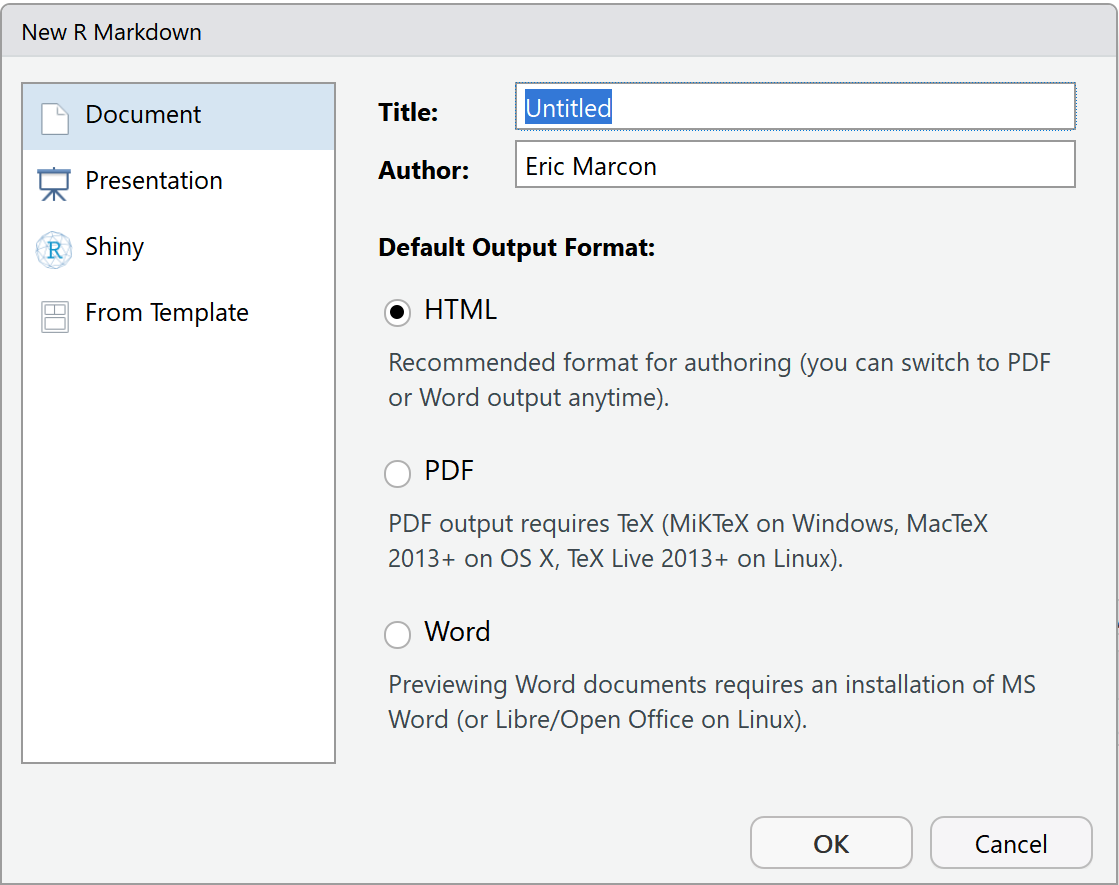
\includegraphics[width=0.8\linewidth]{images/e-rmd1} 

}

\caption{Nouveau document Markdown à partir d'un modèle.}\label{fig:e-rmd1}
\end{figure}

\normalsize

Les modèles les plus simples sont \emph{Document} et \emph{Presentation}.
Les informations à fournir sont le titre et le nom de l'auteur, et le format du document attendu (qui pourra être modifié plus tard).
Ces modèles créent un seul fichier dont l'enregistrement ne sera obligatoire qu'au moment de tricoter.

La syntaxe est la même que celle du bloc-note.
Dans l'entête, une entrée supplémentaire est utilisée pour la date, qui peut être calculée par R à chaque tricot:

\begin{verbatim}
date: "|r format(Sys.Date(), '%d/%m/%Y')|"
\end{verbatim}

Remplacer les barres verticales \texttt{\textbar{}} de l'exemple ci-dessus par des guillemets inversés: ce document étant écrit avec R Markdown, la date serait calculée et affichée à la place du code si les guillemets inversés étaient utilisés directement.

Le code R en ligne (par opposition aux bouts de code) peut être utilisé partout dans un document R Markdown, y compris dans l'entête pour l'affichage de la date.
Il commence par un guillemet inversé suivi de \texttt{r} et se termine par un autre guillemet inversé.

Les documents peuvent être tricotés au format HTML, PDF (via LaTeX) ou Word.
L'entête du fichier R Markdown est réécrit quand le tricot est lancé par le bouton de RStudio qui place en premier le format de sortie utilisé et l'ajoute si nécessaire.

Les présentations peuvent être tricotées dans deux formats HTML, ioslide\footnote{\url{https://bookdown.org/yihui/rmarkdown/ioslides-presentation.html}} ou Slidy\footnote{\url{https://bookdown.org/yihui/rmarkdown/slidy-presentation.html}}, au format Beamer (PDF)\footnote{\url{https://bookdown.org/yihui/rmarkdown/beamer-presentation.html}} ou en Powerpoint\footnote{\url{https://bookdown.org/yihui/rmarkdown/powerpoint-presentation.html}}.

Le niveau 2 de plan (\texttt{\#\#}) marque le changement de diapositive.

Du code supplémentaire, présenté dans les documentations des formats HTML, permet d'utiliser des fonctionnalités spécifiques.

Ces modèles sont simples mais assez peu utiles: le bloc-note R est plus facile à utiliser que le modèle de document pour des documents minimalistes.
Des modèles plus élaborés sont disponibles.

\section{Articles avec bookdown}\label{articles-avec-bookdown}

R Markdown ne permet pas de rédiger un article scientifique.
La bibliographie ne pose pas de problème parce qu'elle est gérée par pandoc pour les documents HTML ou Word et sous-traitée à LaTeX pour les documents PDF.
Les équations, figures et tableaux sont numérotés par LaTeX mais pas en HTML.
Les références croisées (les renvois à un numéro de figure par exemple) ne sont pas supportés.
Enfin, les légendes de figures ou tableaux ne supportent que du texte brut, sans aucun formatage.

\textbf{bookdown} comble ces manques.
Le package a été conçu pour la rédaction d'ouvrages comportant plusieurs chapitres mais peut être utilisé pour des articles.

Le package \textbf{memoiR} fournit les modèles présentés ici.
Il doit être installé.

\subsection{Ecrire}\label{ecrire}

Les principales caractéristiques de Markdown sont résumées ici.
Une formation rapide et plus complète est proposée par RStudio\footnote{\url{https://rmarkdown.rstudio.com/lesson-1.html}}.

Le texte est écrit sans aucun autre formatage que les les retours à la ligne.
Un simple retour à la ligne n'a aucun effet sur le document produit: il permet de séparer les phrases pour simplifier le suivi du code source par git.

Un saut de ligne marque un changement de paragraphe.

Les différents niveaux de plan sont désignés par le nombre de croisillons correspondant en début de ligne: \texttt{\#} pour un titre de niveau 1, \texttt{\#\#} pour un titre de niveau 2, etc.
Un espace sépare les croisillons et le texte du titre.

Les liste à puces sont marquées par un tiret (suivi d'un espace) en début de ligne.
Un saut de ligne est nécessaire avant le début de la liste mais les éléments de la liste sont séparés par un simple retour à la ligne.
Les listes indentées sont créées en insérant 4 espaces avant le tiret de début de ligne.
Enfin, les listes numérotées sont créées de la même façon en remplaçant les tirets par des nombres, dont la valeur n'a pas d'importance.

Dans le texte, les parties en italique sont entourées par une étoile ou un tiret bas (\texttt{*italique*}), alors que deux étoiles marquent le gras.

\subsubsection{Code R}\label{code-r}

Le code R est inclus dans des bouts de code (\emph{code chunks}) créés facilement en cliquant sur le bouton \enquote{Insert a new code chunk} au-dessus de la fenêtre du code source dans RStudio.
Ils commencent et se terminent par trois guillemets inversés sur une nouvelle ligne.
Ces bouts de code peuvent contenir du code R mais aussi Python par exemple: le type de code est indiqué dans l'entête sur la première ligne, avant le nom du bout de code, puis une liste d'options séparées par des virgules, par exemple:

\begin{verbatim}
```{r cars, echo=TRUE}
```
\end{verbatim}

Le nom et les options sont facultatifs: l'entête minimal est \texttt{\{r\}}.

Les options les plus utiles sont:

\begin{itemize}
\tightlist
\item
  \texttt{echo} pour afficher (\texttt{=TRUE}) ou cacher (\texttt{=FALSE}) le code;
\item
  \texttt{message=FALSE} pour cacher les messages d'ouverture de certains packages;
\item
  \texttt{warning=FALSE} pour cacher les avertissements.
\end{itemize}

Les options par défaut sont déclarées dans le bout de code nommé \enquote{Options} au début du document Markdown, dans la fonction \texttt{opts\_chunk\$set()}.

L'option \texttt{include=FALSE} supprime tout affichage lié au bout de code.
Dans un document tel qu'un article scientifique, qui n'affiche pas son code, elle doit être utilisée pour tous les bouts de code sauf ceux qui produisent les figures.

\subsubsection{Figures}\label{figures}

\scriptsize

\begin{Shaded}
\begin{Highlighting}[]
\FunctionTok{plot}\NormalTok{(pressure)}
\end{Highlighting}
\end{Shaded}

\begin{figure}

{\centering 
\includegraphics[width=0.8\linewidth]{travailleR_files/figure-latex/pressure-1} 

}

\caption{Titre de la figure}\label{fig:pressure}
\end{figure}

\normalsize

Les figures peuvent être créées par le code R (figure \ref{fig:pressure}).
Avec Bookdown, une étiquette est associée à chaque figure: son nom est \texttt{fig:xxx} où \texttt{xxx} est le nom du bout de code R.
Les renvois se font avec la commande \texttt{\textbackslash{}@ref(fig:xxx)}.

L'entête du bout de code de la figure \ref{fig:pressure} est:

\begin{verbatim}
```{r pressure, fig.cap="Titre de la figure"}
```
\end{verbatim}

Il contient au minimum le nom de la figure et sa légende.
Si la légende est longue, l'entête est peu lisible.
De plus, la légende est limitée à du texte simple.
Pour des légendes plus élaborées, il est possible de déclarer la légende dans un paragraphe séparé qui commence par le texte \texttt{(ref:NomFigure)}.
La figure \ref{fig:pressure2} bénéficie d'une légende améliorée.



\scriptsize

\begin{figure}

{\centering 
\includegraphics[width=0.8\linewidth]{travailleR_files/figure-latex/pressure2-1} 

}

\caption{Titre avec \emph{italique}, maths (\(\sqrt\pi\)) et renvoi vers la figure \ref{fig:pressure}}\label{fig:pressure2}
\end{figure}

\normalsize

Le texte de \texttt{fig.cap}, \enquote{Titre de la figure} précédemment, est remplacé par \texttt{(ref:pressure)} \emph{à l'intérieur des guillemets} qui sont conservés et la légende est saisie dans un paragraphe commençant par \texttt{(ref:pressure)} suivi d'un espace.
Les légendes sont limitées à un paragraphe unique.

Si une table des figures est utilisée (option \texttt{lof:\ true} dans l'entête), une légende courte est nécessaire en plus de la légende complète.
Elle est déclarée dans \texttt{fig.scap}.

Les figures qui ne sont pas créées par R mais proviennent de fichiers sont intégrées dans un bout de code par la fonction \texttt{include\_graphics()} dont l'argument est le fichier contenant l'image à afficher.
Placer systématiquement ces fichiers dans le dossier \texttt{images} pour une bonne organisation.

\subsubsection{Tableaux}\label{tableaux}

Les séparateurs horizontaux - et verticaux \textbar{} permettent de dessiner un tableau selon la syntaxe de Markdown, mais ce n'est pas la meilleure méthode.

Les tableaux peuvent aussi être produits par du code R.
Le contenu du tableau est dans un dataframe.
La fonction \texttt{kbl} du package \emph{kableExtra} prépare le tableau pour l'affichage et passe le résultat à la fonction \texttt{kable\_styling} pour le formatage final.

\scriptsize

\begin{Shaded}
\begin{Highlighting}[]
\FunctionTok{library}\NormalTok{(}\StringTok{"tidyverse"}\NormalTok{)}
\NormalTok{mes\_iris }\OtherTok{\textless{}{-}} \FunctionTok{head}\NormalTok{(iris)}
\FunctionTok{names}\NormalTok{(mes\_iris) }\OtherTok{\textless{}{-}} \FunctionTok{c}\NormalTok{(}
  \StringTok{"Longueur sépales ($l\_s$)"}\NormalTok{, }
  \StringTok{"Largeur"}\NormalTok{, }
  \StringTok{"Longueur pétales"}\NormalTok{, }
  \StringTok{"Largeur"}\NormalTok{, }
  \StringTok{"Espèce"}
\NormalTok{)}
\NormalTok{kableExtra}\SpecialCharTok{::}\FunctionTok{kbl}\NormalTok{(}
\NormalTok{  mes\_iris, }
  \AttributeTok{caption =} \StringTok{"Tableau créé par kable"}\NormalTok{, }
  \AttributeTok{booktabs =} \ConstantTok{TRUE}\NormalTok{, }
  \AttributeTok{escape =} \ConstantTok{FALSE}
\NormalTok{) }\SpecialCharTok{\%\textgreater{}\%}
\NormalTok{  kableExtra}\SpecialCharTok{::}\FunctionTok{kable\_styling}\NormalTok{(}
    \AttributeTok{bootstrap\_options =} \StringTok{"striped"}\NormalTok{, }
    \AttributeTok{full\_width =} \ConstantTok{FALSE}
\NormalTok{  )}
\end{Highlighting}
\end{Shaded}

\begin{table}
\centering
\caption{\label{tab:kable}Tableau créé par kable}
\centering
\begin{tabular}[t]{rrrrl}
\toprule
Longueur sépales ($l_s$) & Largeur & Longueur pétales & Largeur & Espèce\\
\midrule
5.1 & 3.5 & 1.4 & 0.2 & setosa\\
4.9 & 3.0 & 1.4 & 0.2 & setosa\\
4.7 & 3.2 & 1.3 & 0.2 & setosa\\
4.6 & 3.1 & 1.5 & 0.2 & setosa\\
5.0 & 3.6 & 1.4 & 0.2 & setosa\\
\addlinespace
5.4 & 3.9 & 1.7 & 0.4 & setosa\\
\bottomrule
\end{tabular}
\end{table}

\normalsize

La légende est précisée par l'argument \texttt{caption} et le référencement est possible parce que le tableau reçoit une étiquette dont le nom est \texttt{tab:} suivi du nom du bout de code (tableau \ref{tab:kable}).
Comme pour les figures, une légende améliorée peut être écrite dans un paragraphe séparé.
Une légende courte pour une éventuelle liste des tableaux (option \texttt{lot:\ true} dans l'entête) est déclarée dans l'argument \texttt{caption.short} de \texttt{kbl()}.

Utiliser systématiquement l'argument \texttt{booktabs\ =\ TRUE} pour que l'épaisseur des lignes de séparation soit optimale en LaTeX.
Comme le tableau contient des mathématiques (dans le nom de la première colonne), l'option \texttt{escape\ =\ FALSE} est nécessaire.

L'option de style \texttt{bootstrap\_options\ =\ "striped"} fournit des tableaux plus lisibles en HTML.
Enfin, l'option \texttt{full\_width\ =\ FALSE} permet d'ajuster la largeur du tableau à son contenu au lieu d'occuper toute la largeur disponible.

Le package \textbf{flextable} permet de réaliser des tableaux plus élaborés, comme dans l'exemple suivant qui affiche en couleur les longs sépales.

\scriptsize

\begin{Shaded}
\begin{Highlighting}[]
\FunctionTok{library}\NormalTok{(}\StringTok{"flextable"}\NormalTok{)}
\CommentTok{\# Rappel du jeu de données initial iris}
\NormalTok{iris }\SpecialCharTok{\%\textgreater{}\%}
  \CommentTok{\# Premières lignes}
  \FunctionTok{head}\NormalTok{() }\SpecialCharTok{\%\textgreater{}\%} 
  \CommentTok{\# Création d\textquotesingle{}un objet flextable}
  \FunctionTok{flextable}\NormalTok{() }\SpecialCharTok{\%\textgreater{}\%}
  \CommentTok{\# Titre des colonnes}
  \FunctionTok{set\_header\_labels}\NormalTok{(}
    \AttributeTok{Sepal.Length =} \StringTok{"Longueur sépales"}\NormalTok{,}
    \AttributeTok{Sepal.Width =} \StringTok{"Largeur"}\NormalTok{, }
    \AttributeTok{Petal.Length =} \StringTok{"Longueur pétales"}\NormalTok{,}
    \AttributeTok{Petal.Width =} \StringTok{"Largeur"}\NormalTok{,}
    \AttributeTok{Species =} \StringTok{"Espèce"}
\NormalTok{  ) }\SpecialCharTok{\%\textgreater{}\%}
  \CommentTok{\# Sélection des longs sépales (\textgreater{}5) et affichage en rouge}
  \FunctionTok{color}\NormalTok{(}\SpecialCharTok{\textasciitilde{}}\NormalTok{Sepal.Length }\SpecialCharTok{\textgreater{}} \DecValTok{5}\NormalTok{, }\SpecialCharTok{\textasciitilde{}}\NormalTok{Sepal.Length, }\AttributeTok{color =} \StringTok{"red"}\NormalTok{)}
\end{Highlighting}
\end{Shaded}

\global\setlength{\Oldarrayrulewidth}{\arrayrulewidth}

\global\setlength{\Oldtabcolsep}{\tabcolsep}

\setlength{\tabcolsep}{2pt}

\renewcommand*{\arraystretch}{1.5}



\providecommand{\ascline}[3]{\noalign{\global\arrayrulewidth #1}\arrayrulecolor[HTML]{#2}\cline{#3}}

\begin{longtable}[c]{|p{0.75in}|p{0.75in}|p{0.75in}|p{0.75in}|p{0.75in}}



\ascline{1.5pt}{666666}{1-5}

\multicolumn{1}{>{\raggedleft}m{\dimexpr 0.75in+0\tabcolsep}}{\textcolor[HTML]{000000}{\fontsize{11}{11}\selectfont{\global\setmainfont{Helvetica}{Longueur\ sépales}}}} & \multicolumn{1}{>{\raggedleft}m{\dimexpr 0.75in+0\tabcolsep}}{\textcolor[HTML]{000000}{\fontsize{11}{11}\selectfont{\global\setmainfont{Helvetica}{Largeur}}}} & \multicolumn{1}{>{\raggedleft}m{\dimexpr 0.75in+0\tabcolsep}}{\textcolor[HTML]{000000}{\fontsize{11}{11}\selectfont{\global\setmainfont{Helvetica}{Longueur\ pétales}}}} & \multicolumn{1}{>{\raggedleft}m{\dimexpr 0.75in+0\tabcolsep}}{\textcolor[HTML]{000000}{\fontsize{11}{11}\selectfont{\global\setmainfont{Helvetica}{Largeur}}}} & \multicolumn{1}{>{\raggedright}m{\dimexpr 0.75in+0\tabcolsep}}{\textcolor[HTML]{000000}{\fontsize{11}{11}\selectfont{\global\setmainfont{Helvetica}{Espèce}}}} \\

\ascline{1.5pt}{666666}{1-5}\endfirsthead 

\ascline{1.5pt}{666666}{1-5}

\multicolumn{1}{>{\raggedleft}m{\dimexpr 0.75in+0\tabcolsep}}{\textcolor[HTML]{000000}{\fontsize{11}{11}\selectfont{\global\setmainfont{Helvetica}{Longueur\ sépales}}}} & \multicolumn{1}{>{\raggedleft}m{\dimexpr 0.75in+0\tabcolsep}}{\textcolor[HTML]{000000}{\fontsize{11}{11}\selectfont{\global\setmainfont{Helvetica}{Largeur}}}} & \multicolumn{1}{>{\raggedleft}m{\dimexpr 0.75in+0\tabcolsep}}{\textcolor[HTML]{000000}{\fontsize{11}{11}\selectfont{\global\setmainfont{Helvetica}{Longueur\ pétales}}}} & \multicolumn{1}{>{\raggedleft}m{\dimexpr 0.75in+0\tabcolsep}}{\textcolor[HTML]{000000}{\fontsize{11}{11}\selectfont{\global\setmainfont{Helvetica}{Largeur}}}} & \multicolumn{1}{>{\raggedright}m{\dimexpr 0.75in+0\tabcolsep}}{\textcolor[HTML]{000000}{\fontsize{11}{11}\selectfont{\global\setmainfont{Helvetica}{Espèce}}}} \\

\ascline{1.5pt}{666666}{1-5}\endhead



\multicolumn{1}{>{\raggedleft}m{\dimexpr 0.75in+0\tabcolsep}}{\textcolor[HTML]{FF0000}{\fontsize{11}{11}\selectfont{\global\setmainfont{Helvetica}{5.1}}}} & \multicolumn{1}{>{\raggedleft}m{\dimexpr 0.75in+0\tabcolsep}}{\textcolor[HTML]{000000}{\fontsize{11}{11}\selectfont{\global\setmainfont{Helvetica}{3.5}}}} & \multicolumn{1}{>{\raggedleft}m{\dimexpr 0.75in+0\tabcolsep}}{\textcolor[HTML]{000000}{\fontsize{11}{11}\selectfont{\global\setmainfont{Helvetica}{1.4}}}} & \multicolumn{1}{>{\raggedleft}m{\dimexpr 0.75in+0\tabcolsep}}{\textcolor[HTML]{000000}{\fontsize{11}{11}\selectfont{\global\setmainfont{Helvetica}{0.2}}}} & \multicolumn{1}{>{\raggedright}m{\dimexpr 0.75in+0\tabcolsep}}{\textcolor[HTML]{000000}{\fontsize{11}{11}\selectfont{\global\setmainfont{Helvetica}{setosa}}}} \\





\multicolumn{1}{>{\raggedleft}m{\dimexpr 0.75in+0\tabcolsep}}{\textcolor[HTML]{000000}{\fontsize{11}{11}\selectfont{\global\setmainfont{Helvetica}{4.9}}}} & \multicolumn{1}{>{\raggedleft}m{\dimexpr 0.75in+0\tabcolsep}}{\textcolor[HTML]{000000}{\fontsize{11}{11}\selectfont{\global\setmainfont{Helvetica}{3.0}}}} & \multicolumn{1}{>{\raggedleft}m{\dimexpr 0.75in+0\tabcolsep}}{\textcolor[HTML]{000000}{\fontsize{11}{11}\selectfont{\global\setmainfont{Helvetica}{1.4}}}} & \multicolumn{1}{>{\raggedleft}m{\dimexpr 0.75in+0\tabcolsep}}{\textcolor[HTML]{000000}{\fontsize{11}{11}\selectfont{\global\setmainfont{Helvetica}{0.2}}}} & \multicolumn{1}{>{\raggedright}m{\dimexpr 0.75in+0\tabcolsep}}{\textcolor[HTML]{000000}{\fontsize{11}{11}\selectfont{\global\setmainfont{Helvetica}{setosa}}}} \\





\multicolumn{1}{>{\raggedleft}m{\dimexpr 0.75in+0\tabcolsep}}{\textcolor[HTML]{000000}{\fontsize{11}{11}\selectfont{\global\setmainfont{Helvetica}{4.7}}}} & \multicolumn{1}{>{\raggedleft}m{\dimexpr 0.75in+0\tabcolsep}}{\textcolor[HTML]{000000}{\fontsize{11}{11}\selectfont{\global\setmainfont{Helvetica}{3.2}}}} & \multicolumn{1}{>{\raggedleft}m{\dimexpr 0.75in+0\tabcolsep}}{\textcolor[HTML]{000000}{\fontsize{11}{11}\selectfont{\global\setmainfont{Helvetica}{1.3}}}} & \multicolumn{1}{>{\raggedleft}m{\dimexpr 0.75in+0\tabcolsep}}{\textcolor[HTML]{000000}{\fontsize{11}{11}\selectfont{\global\setmainfont{Helvetica}{0.2}}}} & \multicolumn{1}{>{\raggedright}m{\dimexpr 0.75in+0\tabcolsep}}{\textcolor[HTML]{000000}{\fontsize{11}{11}\selectfont{\global\setmainfont{Helvetica}{setosa}}}} \\





\multicolumn{1}{>{\raggedleft}m{\dimexpr 0.75in+0\tabcolsep}}{\textcolor[HTML]{000000}{\fontsize{11}{11}\selectfont{\global\setmainfont{Helvetica}{4.6}}}} & \multicolumn{1}{>{\raggedleft}m{\dimexpr 0.75in+0\tabcolsep}}{\textcolor[HTML]{000000}{\fontsize{11}{11}\selectfont{\global\setmainfont{Helvetica}{3.1}}}} & \multicolumn{1}{>{\raggedleft}m{\dimexpr 0.75in+0\tabcolsep}}{\textcolor[HTML]{000000}{\fontsize{11}{11}\selectfont{\global\setmainfont{Helvetica}{1.5}}}} & \multicolumn{1}{>{\raggedleft}m{\dimexpr 0.75in+0\tabcolsep}}{\textcolor[HTML]{000000}{\fontsize{11}{11}\selectfont{\global\setmainfont{Helvetica}{0.2}}}} & \multicolumn{1}{>{\raggedright}m{\dimexpr 0.75in+0\tabcolsep}}{\textcolor[HTML]{000000}{\fontsize{11}{11}\selectfont{\global\setmainfont{Helvetica}{setosa}}}} \\





\multicolumn{1}{>{\raggedleft}m{\dimexpr 0.75in+0\tabcolsep}}{\textcolor[HTML]{000000}{\fontsize{11}{11}\selectfont{\global\setmainfont{Helvetica}{5.0}}}} & \multicolumn{1}{>{\raggedleft}m{\dimexpr 0.75in+0\tabcolsep}}{\textcolor[HTML]{000000}{\fontsize{11}{11}\selectfont{\global\setmainfont{Helvetica}{3.6}}}} & \multicolumn{1}{>{\raggedleft}m{\dimexpr 0.75in+0\tabcolsep}}{\textcolor[HTML]{000000}{\fontsize{11}{11}\selectfont{\global\setmainfont{Helvetica}{1.4}}}} & \multicolumn{1}{>{\raggedleft}m{\dimexpr 0.75in+0\tabcolsep}}{\textcolor[HTML]{000000}{\fontsize{11}{11}\selectfont{\global\setmainfont{Helvetica}{0.2}}}} & \multicolumn{1}{>{\raggedright}m{\dimexpr 0.75in+0\tabcolsep}}{\textcolor[HTML]{000000}{\fontsize{11}{11}\selectfont{\global\setmainfont{Helvetica}{setosa}}}} \\





\multicolumn{1}{>{\raggedleft}m{\dimexpr 0.75in+0\tabcolsep}}{\textcolor[HTML]{FF0000}{\fontsize{11}{11}\selectfont{\global\setmainfont{Helvetica}{5.4}}}} & \multicolumn{1}{>{\raggedleft}m{\dimexpr 0.75in+0\tabcolsep}}{\textcolor[HTML]{000000}{\fontsize{11}{11}\selectfont{\global\setmainfont{Helvetica}{3.9}}}} & \multicolumn{1}{>{\raggedleft}m{\dimexpr 0.75in+0\tabcolsep}}{\textcolor[HTML]{000000}{\fontsize{11}{11}\selectfont{\global\setmainfont{Helvetica}{1.7}}}} & \multicolumn{1}{>{\raggedleft}m{\dimexpr 0.75in+0\tabcolsep}}{\textcolor[HTML]{000000}{\fontsize{11}{11}\selectfont{\global\setmainfont{Helvetica}{0.4}}}} & \multicolumn{1}{>{\raggedright}m{\dimexpr 0.75in+0\tabcolsep}}{\textcolor[HTML]{000000}{\fontsize{11}{11}\selectfont{\global\setmainfont{Helvetica}{setosa}}}} \\

\ascline{1.5pt}{666666}{1-5}



\end{longtable}



\arrayrulecolor[HTML]{000000}

\global\setlength{\arrayrulewidth}{\Oldarrayrulewidth}

\global\setlength{\tabcolsep}{\Oldtabcolsep}

\renewcommand*{\arraystretch}{1}

\normalsize

La documentation du package\footnote{\url{https://ardata-fr.github.io/flextable-book/}} est disponible en ligne, ainsi qu'une galerie\footnote{\url{https://ardata-fr.github.io/flextable-gallery/gallery/}}.

\textbf{flextable} ne supporte pas la numérotation des légendes hormis dans les documents Word.
Cette limite est rédhibitoire.

\subsubsection{Maths}\label{maths}

Les équations au format LaTeX peuvent être insérées en ligne, comme \(A=\pi r^2\) (code: \texttt{\$A=\textbackslash{}pi\ r\^{}2\$}) ou isolées (les \$ sont doublés) comme \[e^{i \pi} = -1.\]

Elles peuvent être numérotées: voir équation \eqref{eq:disque}, en utilisant l'environnement \texttt{\textbackslash{}equation}.

\begin{equation}
  A = \pi r^2.
  \label{eq:disque}
\end{equation}

L'équation numérotée est créée par le code suivant:

\begin{verbatim}
\begin{equation}
  A = \pi r^2.
  \label{eq:disque}
\end{equation}
\end{verbatim}

\subsubsection{Références croisées}\label{ruxe9fuxe9rences-croisuxe9es}

Les figures et tableaux ont une étiquette générée automatiquement, identique au nom du bout de code préfixé par \texttt{fig:} et \texttt{tab:}.

Pour les équations, l'étiquette est ajoutée manuellement par le code \texttt{(\textbackslash{}\#eq:xxx)} avant la fin de l'équation.

Les sections peuvent recevoir une étiquette en terminant leur titre par \texttt{\{\#yyy\}}.
Les sections reçoivent par défaut une étiquette implicite\footnote{\url{https://pandoc.org/MANUAL.html\#extension-implicit_header_references}} correspondant à leur texte, en minuscules, où les caractères spéciaux sont remplacés par des tirets.
Les étiquettes implicites sont instables (elles changent avec le titre de la section) et difficiles à prévoir: c'est pourquoi il est conseillé d'ajouter une étiquette explicite à chaque section faisant l'objet d'un renvoi.
C'est le cas des chapitres, pour lesquels le nom du fichier HMTL produit est identique à l'étiquette.
Les étiquettes de chapitres doivent respecter les règles de nomenclature des fichiers en ne contenant pas de caractères spéciaux.

Des signets peuvent aussi être placés librement dans le texte avec la commande \texttt{(ref:zzz)}.

Dans tous les cas, l'appel à la référence est fait par la commande \texttt{\textbackslash{}@ref(ref:zzz)}.

\subsubsection{Bibliographie}\label{bibliographie}

Les références bibliographiques au format BibTeX doivent être incluses dans le fichier \texttt{.bib} déclaré dans l'entête du document Markdown.

\begin{verbatim}
bibliography: references.bib
\end{verbatim}

Ce fichier peut être créé et maintenu à jour par Zotero installé avec l'extension Better BibTeX (voir section \ref{sec:Zotero}).
Il suffit pour cela de créer une collection Zotero correspondant au projet et d'y glisser les références pertinentes.
Utiliser ensuite le menu contextuel \enquote{Exporter la collection\ldots{}} et sélectionner:

\begin{itemize}
\tightlist
\item
  Format: \enquote{Better BibTeX} pour les articles et présentations ou \enquote{Better BibLaTeX} pour les mémoires, selon que la bibliographie est gérée par BibTeX et natbib ou biber et BibLaTeX pour la production de documents PDF.
\item
  Cocher la case \enquote{Garder à jour} pour que toute modification dans Zotero soit exportée automatiquement.
\item
  Cliquer sur \enquote{OK} puis choisir le nom du fichier (\texttt{references.bib}) et son emplacement (le dossier du projet R).
\end{itemize}

Les références peuvent être appelées dans le texte, entre parenthèses par le code \texttt{{[}@Reference{]}}, ou dans le texte, en supprimant les crochets.

La bibliographie est traitée par pandoc lors de la production de documents Word ou HTML.
Le style bibliographique peut être précisé, en ajoutant la ligne

\begin{verbatim}
csl:nom_du_fichier.csl
\end{verbatim}

dans l'entête du document et en copiant le fichier de style \emph{.csl} dans le dossier du projet.
Plus d'un millier de styles sont disponibles\footnote{\url{https://github.com/citation-style-language/styles}}.

Pour les documents PDF, la bibliographie est gérée par LaTeX.

Pour préparer la soumission d'un manuscrit à une revue, il faudra ouvrir le fichier \emph{.tex} intermédiaire produit par pandoc et copier le contenu de l'environnement \{document\} dans le modèle proposé par la revue, qui se chargera du formatage.

\subsubsection{Langues}\label{langues}

Les langues sont à déclarer dans l'entête des document produits par les modèles de \textbf{memoiR}.

La langue principale du document modifie le nom de certains éléments, comme la table des matières.
Les langues supplémentaires permettent la rédaction de documents multilingues.

Les champs de l'entête sont:

\begin{verbatim}
lang: fr-FR
otherlangs: [en-US, it]
\end{verbatim}

Le changement de langue dans le document est géré en LaTeX mais pas en HTML en insérant sur une nouvelle ligne la commande suivante:

\begin{verbatim}
\selectlanguage{english}
\end{verbatim}

La langue en cours n'a d'effet que dans les sorties LaTeX: un espace est ajouté devant les ponctuations doubles en Français, la taille des espaces est plus grande en début de phrase en Anglais, etc.
La commande \texttt{\textbackslash{}selectlanguage} est simplement ignorée en HTML.

Les noms de langues sont différents dans l'entête (codes IETF) et dans le texte (nom de la langue).
La correspondance et la liste complète des langues se trouve dans le tableau 3 de la documentation du package \textbf{polyglossia}\footnote{\url{http://mirrors.ctan.org/macros/unicodetex/latex/polyglossia/polyglossia.pdf}}.

Le formatage en HTML de la ponctuation des documents en français est possible par l'intermédiaire d'un filtre déclaré à pandoc \footnote{\url{https://github.com/InseeFrLab/pandoc-filter-fr-nbsp}}.
Le fichier \texttt{fr-nbsp.lua} doit être copié dans le répertoire du projet à partir de son dépôt GitHub et éclaré dans l'entête du document Markdown.

\begin{verbatim}
output:
    pandoc_args:
      - --lua-filter=fr-nbsp.lua
\end{verbatim}

Le filtre formate toute la ponctuation du document, quelle que soit sa langue: il ne doit donc être utilisé que pour les documents entièrement en français.

\subsection{Modèle Simple Article}\label{sec:memo}

Le modèle \emph{Simple Article} de \textbf{memoiR} produit un document HTML simple avec une table des matières flottante (voir l'exemple\footnote{\url{https://EricMarcon.github.io/Krigeage/Krigeage.html}}).
D'autres formats HTML sont disponibles: voir la gallerie\footnote{\url{https://ericmarcon.github.io/memoiR/}} du package.
Le format PDF est proche du modèle \emph{article} de LaTeX (exemple\footnote{\url{https://EricMarcon.github.io/Krigeage/Krigeage.pdf}}).

Le modèle contient sa propre documentation.

\subsubsection{Créer}\label{cruxe9er}

Utiliser le menu \enquote{File \textgreater{} New File \textgreater{} R Markdown\ldots{}} puis sélectionner \enquote{From template} (figure \ref{fig:e-rmd1}).
La liste des modèles disponible et le package qui les propose est alors affichée.

Sélectionner le modèle \emph{Simple Article} du package \textbf{memoiR}, choisir le nom du projet (\enquote{Name:}, qui sera le nom du dossier dans lequel il sera créé, et son dossier parent (\enquote{Location:}).
Dans l'organisation proposée en section \ref{sec:solution-dossiers}, le dossier parent est \texttt{\%LOCALAPPDATA\%\textbackslash{}ProjetsR}.
Le nom du projet ne doit contenir aucun caractère spécial (accent, espace\ldots) pour assurer sa portabilité sur tous les systèmes d'exploitation (Windows, Linux, MacOS).

Les modèles élaborés créent un dossier avec de nombreux fichiers (bibliographie, styles, modèle LaTeX\ldots), contrairement aux modèles simples qui créent seulement un fichier.

Quand un dossier est créé, par exemple par le modèle \emph{Simple Article}, il faut en faire un projet RStudio: dans le menu des projets (en haut à droite de la fenêtre de RStudio), utiliser le menu \enquote{New Project\ldots{}} puis \enquote{Existing Directory} et sélectionner le dossier qui vient d'être créé.

\subsubsection{Ecrire}\label{ecrire-1}

Les instructions pour utiliser le modèle sont contenues dans le texte fourni par défaut.

\subsubsection{Tricoter}\label{tricoter}

Le document peut être tricoté en plusieurs formats:

\begin{itemize}
\tightlist
\item
  \emph{html\_document2} est le format HTML pour lequel le modèle a été conçu: un bloc-note avec une table des matières flottante;
\item
  \emph{gitbook} est un format HTML alternatif, utilisé normalement pour les ouvrages;
\item
  \emph{downcute} est un format HTML proposé par le package \textbf{rmdformats};
\item
  \emph{pdf\_book} produit un document PDF suivant le modèle LaTeX \emph{article}, couramment utilisé directement en LaTeX;
\item
  \emph{word\_document2} crée un ficher Word.
\end{itemize}

\subsubsection{Mettre en ligne}\label{sec:article-en-ligne}

Le package \textbf{memoiR} simplifie la mise en ligne des documents produits.

La fonction \texttt{build\_gitignore()} crée un fichier \texttt{.gitignore} pour le contrôle de source qui doit être activé (voir section \ref{sec:git-cds}).

La fonction \texttt{build\_readme()} crée un fichier \texttt{README.md} nécessaire à GitHub.
Il contient le titre du projet, son résumé et des liens vers les versions HTML et PDF des documents produits.

Le projet doit être lié à un dépôt GitHub (section \ref{sec:creerdepot}).

Deux stratégies de publications sont possible.
Dans la première, les documents sont tricotés localement et placés dans le dossier \texttt{docs}, qui sera le support des pages GitHub.
Dans la seconde, les documents sont tricotés par GitHub Actions à chaque fois que des modifications sont poussées sur le dépôt: on parle d'intégration continue (section \ref{chap-ci}).

La stratégie de production locale est traitée ici; l'intégration continue le sera dans la section \ref{sec:memoiR-ci}.

La fonction \texttt{build\_githubpages()} place tous les documents tricotés (HTML et PDF) dans le dossier \texttt{docs}, avec une copie du fichier \texttt{README.md}.
De cette façon, il est possible d'activer les pages GitHub du projet (sur le dossier \texttt{docs} de la branche \texttt{master}).
Le fichier \texttt{README.md} sera la page d'accueil du site web produit.

En pratique, on tricote au format HTML pendant toute la phase de rédaction, parce que la production est très rapide.
Quand le document est stabilisé, il faut le tricoter au format HTML et au format PDF.
Enfin, l'exécution de \texttt{build\_githubpages()} place tous les fichiers produits dans \texttt{docs}.
Il reste à pousser le dépôt sur GitHub et activer les pages GitHub.

\subsection{Autres modèles}\label{autres-moduxe8les}

Le modèle \emph{Stylish Article} de \textbf{memoiR} est destiné à la production d'articles PDF pour l'autoarchivage (typiquement, le dépôt sur HAL) bien formatés, au format A4 en double colonne\footnote{Exemple: \url{https://EricMarcon.github.io/Rochebrune2018/Entropie.pdf}}.

Le format HTML est le même que celui du modèle \emph{Simple Article}.

Le package \textbf{rticles} a pour ambition de fournir des modèles pour toutes les revues scientifiques qui acceptent une soumission d'articles en LaTeX.
Il propose donc des modèles Markdown qui produisent des fichiers PDF conformes aux exigences des revues et la possibilité de récupérer le fichier \texttt{.tex} intermédiaire (pandoc produit un fichier \texttt{.tex} transmis au compilateur LaTeX).
Le package ne permet pas de tricot HTML parce qu'il utilise la syntaxe LaTeX dans le document R Markdown au lieu d'utiliser \textbf{bookdown} pour gérer les références bibliographique et les références croisées.
Il n'est pas possible d'échanger directement du contenu R Markdown standard avec des documents écrits pour \textbf{rticles}, ce qui limite beaucoup l'intérêt du package.

\section{Présentation Beamer}\label{pruxe9sentation-beamer}

Le modèle \emph{Beamer Presentation} de \textbf{memoiR} permet de créer des présentations au format HTML et PDF (beamer) simultanément, comme le montre l'exemple\footnote{\url{https://EricMarcon.github.io/Chao1/}, choisir Lecture (HTML) ou Téléchargement (PDF).}.

La démarche est identique à celle des articles du même package.
Les niveaux de titre permettent de séparer les parties de la présentation (\texttt{\#}) et les diapositives (\texttt{\#\#}).
Deux formats sont disponibles en HTML: ioslides\footnote{\url{https://bookdown.org/yihui/rmarkdown/ioslides-presentation.html}} et Slidy\footnote{\url{https://bookdown.org/yihui/rmarkdown/slidy-presentation.html}}.
Quelques spécificités dans le code permettent d'affiner la présentation des diapositives, pour un affichage sur deux colonnes par exemple: elles sont documentées dans le modèle.

\section{memoir}\label{memoir}

Le modèle \emph{Memoir} du package \textbf{memoiR} est destiné aux documents longs, qui présentent une différence importante avec les documents précédents: un document long est composé de plusieurs chapitres, chacun placé dans son fichier \texttt{.Rmd}.

Le format HTML est gitbook\footnote{\url{https://www.gitbook.com/}}, le standard de la lecture en ligne de documents de ce type.
Le format PDF est dérivé du modèle LaTeX \emph{memoir}\footnote{\url{https://www.ctan.org/pkg/memoir}}, optimisé aussi pour les documents longs.

Ce document a été écrit avec ce modèle.

\subsection{Créer}\label{cruxe9er-1}

La création d'un projet d'ouvrage est identique à celle présentée plus haut: le modèle est: \emph{Memoir}.
Le dossier créé doit être transformé en projet.

Exécuter \texttt{build\_git()} et \texttt{build\_readme()}, activer le contrôle de source et pousser le projet sur GitHub, de la même façon que pour un article (section \ref{sec:article-en-ligne}).

Chaque chapitre de l'ouvrage est un fichier Rmd, dont le nom commence normalement par son numéro (ex.: \texttt{01-intro.Rmd}).
Tous les fichiers Rmd présents dans le dossier du projet sont en réalité traités comme des chapitres, triés par ordre de nom de fichier, dont ceux fournis par le modèle (démarrage et syntaxe) qui doivent être supprimés à l'exception de \texttt{99-references.Rmd} qui contient la bibliographie, placée à la fin.
Le fichier \texttt{index.Rmd} est particulier: il contient l'entête du document et le premier chapitre.

\subsection{Ecrire}\label{ecrire-2}

Le premier chapitre est placé dans l'avant-propos de l'ouvrage imprimé: il ne doit pas être numéroté (d'où le code \texttt{\{-\}} à côté du titre) dans la version HTML.
Il se termine obligatoirement par la commande LaTeX \texttt{\textbackslash{}mainmatter} qui marque le début du corps de l'ouvrage.

Les niveaux de plan commencent par \texttt{\#} pour les chapitres (un seul par fichier), \texttt{\#\#} pour les sections, etc.

\subsection{Tricoter}\label{tricoter-1}

La compilation au format PDF est faite par XeLaTeX, qui doit être installé.

Pendant la rédaction, il est fortement conseillé de ne créer que le fichier HTML, ce qui est beaucoup plus rapide qu'une compilation LaTeX.
Chaque chapitre peut être visualisé très rapidement en cliquant sur le bouton \enquote{Knit} au-dessus de la fenêtre de source.
Le livre entier est créé en cliquant sur le bouton \enquote{Build Book} de la fenêtre \emph{Build} de RStudio.
La liste déroulante du bouton permet de créer tous les documents ou de se limiter à un format.

Les fichiers produits sont placés directement dans le dossier \texttt{docs}, qui sera utilisé par les pages GitHub pour permettre la lecture en ligne et le téléchargement du PDF.
La page d'accueil du site web est créée par bookdown à partir du fichier \texttt{index.Rmd}: le fichier \texttt{README.md} n'est pas dupliqué dans \texttt{docs}.

\subsection{Finitions}\label{finitions}

La mise en page est assurée de façon totalement automatique par pandoc (en HTML) et LaTeX (en PDF).

Il est souvent utile d'aider LaTeX à résoudre quelques dépassements de marge dus à de trop grandes contraintes de mise en page: pour la lisibilité optimale, les colonnes sont étroites, mais le code (texte formaté entre deux apostrophes inversées) n'autorise pas la césure.

Si une ligne de texte dépasse dans la marge de droite dans le document PDF, la solution consiste à ajouter manuellement le code \texttt{\textbackslash{}break} à l'emplacement désiré pour le retour à la ligne dans le document R Markdown.
La commande n'a aucun effet sur le document HTML mais force la césure en LaTeX.
Pour couper du texte formaté (entre astérisques pour l'italique ou plus fréquemment entre apostrophes inversées pour du code), il faut terminer le formatage avant \texttt{\textbackslash{}break} et le recommencer après.
Exemple, pour forcer le retour à la ligne avant \texttt{fichier.Rmd}:

\begin{verbatim}
Le fichier `/chemin/`\break`fichier.Rmd`
\end{verbatim}

En HTML, un espace sera ajouté entre les deux portions de code.

Les bouts de code R sont formatés automatiquement par \textbf{knitr} quand l'option \texttt{tidy=TRUE} leur est appliquée.
Le comportement par défaut est indiqué dans les options de \textbf{knitr}, dans un bout de code au début du fichier \texttt{index.Rmd}:

\scriptsize

\begin{Shaded}
\begin{Highlighting}[]
\CommentTok{\# knitr options}
\NormalTok{knitr}\SpecialCharTok{::}\NormalTok{opts\_chunk}\SpecialCharTok{$}\FunctionTok{set}\NormalTok{(}
  \AttributeTok{cache =} \ConstantTok{TRUE}\NormalTok{, }\AttributeTok{warning =} \ConstantTok{FALSE}\NormalTok{, }\AttributeTok{echo =} \ConstantTok{TRUE}\NormalTok{,}
  \AttributeTok{fig.env =} \StringTok{\textquotesingle{}SCfigure\textquotesingle{}}\NormalTok{, }\AttributeTok{fig.asp =}\NormalTok{ .}\DecValTok{75}\NormalTok{, }
  \AttributeTok{fig.align =} \StringTok{\textquotesingle{}center\textquotesingle{}}\NormalTok{, }\AttributeTok{out.width =} \StringTok{\textquotesingle{}80\%\textquotesingle{}}\NormalTok{, }
  \AttributeTok{tidy =} \ConstantTok{TRUE}\NormalTok{, }
  \AttributeTok{tidy.opts =} \FunctionTok{list}\NormalTok{(}\AttributeTok{blank =} \ConstantTok{FALSE}\NormalTok{, }\AttributeTok{width.cutoff =} \DecValTok{55}\NormalTok{), }
  \AttributeTok{size =} \StringTok{"scriptsize"}\NormalTok{, }
  \AttributeTok{knitr.graphics.auto\_pdf =} \ConstantTok{TRUE}
\NormalTok{)}
\end{Highlighting}
\end{Shaded}

\normalsize

La largeur maximale d'une ligne de code formaté est ici de 55 caractères, optimal pour le modèle.
Il arrive que le formatage automatique ne fonctionne pas parce que \textbf{knitr} ne parvient pas à trouver une coupure de ligne respectant toutes les contraintes, ce qui provoque un dépassement de marge dans le code.
Dans ce cas, formater manuellement le bout de code en lui ajoutant l'option \texttt{tidy=FALSE}.

Les blocs de code littéral, délimités par trois apostrophes inversées, doivent être formatés manuellement, en évitant toute ligne de plus de 55 caractères.

\subsection{Site gitbook}\label{site-gitbook}

Le site web contenant le document gitbook doit être paramétré dans \texttt{\_output.yml} pour que:

\begin{itemize}
\tightlist
\item
  le titre du document apparaisse en haut de la table des matières;
\item
  une indication de l'usage de GitHub et bookdown soit affichée en bas de la table des matières;
\item
  un bouton GitHub dans la barre de titre permette d'ouvrir le dépôt du projet;
\item
  un autre bouton permette de télécharger le document PDF.
\end{itemize}

Le fichier \texttt{\_output.yml} de ce document est le suivant:

\begin{verbatim}
bookdown::gitbook:
  css: style.css
  config:
    sharing:
      github: yes
      facebook: false
      twitter: false
    toc:
      before: |
        <li><a href="./">Travailler avec R</a></li>
      after: |
        <li>
          <a href="https://github.com/EricMarcon/travailleR" target="blank">
            Hébergé sur GitHub, publié par bookdown
          </a>
        </li>
    download: pdf
\end{verbatim}

La section \texttt{sharing:} gère les boutons de la barre de titre.
Par défaut, les liens vers Facebook et Twitter sont activés mais celui vers GitHub ne l'est pas.
Pour qu'il fonctionne, le dépôt GitHub doit être déclaré dans l'entête du fichier \texttt{index.rmd}:

\begin{verbatim}
github-repo: EricMarcon/travailleR
\end{verbatim}

La section \texttt{toc:} contient deux portions de code HTML dans lesquelles le titre du document et le lien vers son dépôt GitHub doivent être adaptés au projet.

Enfin, la section \texttt{download:} liste les formats de documents téléchargeables et permet d'afficher un bouton de téléchargement dans la barre de titre.

\subsection{Intégration continue}\label{sec:rediger-ouvrage-ci}

La construction d'un ouvrage prend du temps, surtout s'il contient des calculs.
Elle doit être lancée au format gitbook et au format PDF.
En production, elle peut être confiée à GitHub (chapitre \ref{sec:bookdown-ci}).

\subsection{Google Analytics}\label{google-analytics}

Le suivi de l'audience de l'ouvrage peut être confié à Google Analytics.
Pour cela, il faut créer un compte et ajouter une \emph{propriété} Google Analytics, c'est-à-dire un site web, puis un flux de données, ici un flux web\footnote{\url{https://support.google.com/analytics/answer/9304153?hl=fr&ref_topic=9303319}}.

Google Analytics fournit un script de configuration nommé \texttt{gtag.js} à placer à la racine du dossier du projet.
Enfin, déclarer le script dans l'entête des pages web en ajoutant une instruction dans \texttt{\_output.yml}, dans sa première section.

\begin{verbatim}
bookdown::gitbook:
  includes:
    in_header: gtag.js
\end{verbatim}

\section{Site web R Markdown}\label{site-web-r-markdown}

Un site web constitué de pages écrites avec R Markdown (sans les fonctionnalités de \textbf{bookdown}) et un menu peut être créé très simplement, avec un résultat de bonne facture\footnote{\url{https://rstudio.github.io/learnr/} par exemple.}.

\subsection{Modèle}\label{moduxe8le}

Dans RStudio, dans le menu des projets en haut à droite, cliquer sur \enquote{New Project\ldots{}} puis \enquote{New Directory} puis \enquote{Simple R Markdown website}.
Saisir le nom du projet, sélectionner le dossier dans lequel le projet sera créé en cliquant sur \enquote{Browse} et enfin cliquer sur \enquote{Create Project}.

Le site par défaut contient deux pages: \texttt{index}, la page d'accueil, et \texttt{about}, la page \enquote{A propos}.
Le fichier \texttt{\_site.yml} contient le nom du site et le contenu de sa barre de navigation: un titre et le fichier correspondant.
D'autres pages seront ajoutées en créant de nouveaux fichiers \texttt{.Rmd} et en les ajoutant au fichier \texttt{\_site.yml}.

\subsection{Améliorations}\label{amuxe9liorations}

Le modèle de site peut facilement être amélioré en complétant \texttt{\_site.yml}:

\begin{itemize}
\tightlist
\item
  en ajoutant une icône GitHub dans la barre de navigation pour renvoyer vers le code source du site;
\item
  en choisissant la méthode de tricot des pages, pour utiliser \textbf{bookdown} au lieu de \textbf{rmarkdown};
\item
  en plaçant les fichiers du site dans le dossier \texttt{docs} et ainsi séparer le code et la production.
\end{itemize}

Le fichier \texttt{\_site.yml} complété est le suivant:

\begin{verbatim}
name: "my-website"
navbar:
  title: "My Website"
  left:
    - text: "Home"
      href: index.html
    - text: "About"
      href: about.html
  right:
    - icon: fa-github
      href: https://github.com/rstudio/rmarkdown
output_dir: "docs"
output:
  bookdown::html_document2:
    theme: sandstone
    highlight: tango
    toc: true
    toc_float: yes
\end{verbatim}

L'icône de GitHub fait partie de la collection Font Awesome dont toutes les icônes gratuites\footnote{\url{https://fontawesome.com/icons?d=gallery&m=free}} sont utilisables avec la même syntaxe: \enquote{fa-nom}.

Le lien correspondant à l'icône doit être celui du dépôt GitHub du site web.

La syntaxe de la section \texttt{output} est la même que celle des documents vus plus haut.
Elle s'applique à toutes les pages (dont l'entête YAML est réduite au minimum).
Les thèmes disponibles sont ceux de rmarkdown\footnote{\url{https://bookdown.org/yihui/rmarkdown/html-document.html\#appearance-and-style}}.

L'option \texttt{highlight} indique la façon dont le code R éventuellement affiché sera formaté.
Enfin, la table des matières est flottante, ce qui signifie que sa position s'ajuste quand la fenêtre défile.

\subsection{Contôle de source}\label{contuxf4le-de-source}

Le projet doit être placé sous contrôle de source et poussé sur GitHub (chapitre \ref{chap-git}).
Le fichier \texttt{.gitignore} est le suivant:

\begin{verbatim}
# R
.Rbuildignore
.RData
.Rhistory
.Rprofile
.Rproj.user

# Web Site
/_site/
/*_cache/
/*_files/
\end{verbatim}

Activer les pages GitHub (section \ref{sec:github-pages}) sur le dossier \texttt{docs} pour héberger le site.
Ajouter un fichier vide nommé \texttt{.nojekyll} dans \texttt{docs} pour que les pages GitHub ne tentent pas de reformater le site.
On peut utiliser le terminal de RStudio pour exécuter:

\begin{verbatim}
touch docs/.nojekyll
\end{verbatim}

\section{Site web personnel : blogdown}\label{sec:blogdown}

Pour créer une page web personnelle, \emph{Hugo} est un générateur de site statique capable de produire des pages HTML à partir de code Markdown.
Les sites statiques ont l'avantage, en comparaison aux sites dynamiques gérés par un système de gestion de contenu (CMS, par exemple: Wordpress, Joomla, SPIP), d'être portables sur n'importe quel serveur web sans support de base de données ni de code à exécuter côté le serveur (tel que PHP) et d'être très rapides puisque les pages sont créées une seule fois et non à chaque consultation.
Un site Hugo peut être hébergé par exemple sur la page personnelle de tout utilisateur de GitHub dont l'adresse est de la forme \enquote{GitHubID.github.io}.

Hugo propose de nombreux thèmes, qui sont des modèles de structure de sites, donc le thème \textbf{Academic}, destiné aux chercheurs.
Dans RStudio, le package \textbf{blogdown} est prévu pour produire facilement des pages web avec Hugo.
Ces pages peuvent contenir du code R: elles sont très proches d'un article, vu plus haut, dont le contenu peut être facilement copié et collé.
Nous utiliserons donc cette solution, pour un site comme celui proposé en exemple\footnote{\url{https://EricMarcon.github.io/}}.

La structure du site web est simple:

\begin{itemize}
\tightlist
\item
  une page d'accueil, contenant divers composants paramétrables comme la biographie de l'auteur, une sélection de publications, de billets de blogs ou d'autres éléments et un formulaire de contact;
\item
  des pages détaillant les divers éléments (publications, billets, etc.) écrites en R Markdown.
\end{itemize}

\subsection{Installation des outils}\label{installation-des-outils}

La première étape consiste à installer le package \textbf{blogdown} dans R.

\scriptsize

\begin{Shaded}
\begin{Highlighting}[]
\FunctionTok{install.packages}\NormalTok{(}\StringTok{\textquotesingle{}blogdown\textquotesingle{}}\NormalTok{) }
\end{Highlighting}
\end{Shaded}

\normalsize

\textbf{blogdown} est capable d'installer Hugo sous Windows, macOS ou Linux.

\scriptsize

\begin{Shaded}
\begin{Highlighting}[]
\NormalTok{blogdown}\SpecialCharTok{::}\FunctionTok{install\_hugo}\NormalTok{()}
\end{Highlighting}
\end{Shaded}

\normalsize

La documentation complète de \textbf{blogdown} est disponible\footnote{\url{https://bookdown.org/yihui/blogdown/}}.

Les versions récentes de Hugo utilisent \emph{Go} (le langage de programmation) pour installer leurs modules à la volée: ici le thème Academic est chargé depuis GitHub au moment de la création du site.
Go doit donc être installé\footnote{\url{https://golang.org/doc/install}}.

\subsection{Créer}\label{cruxe9er-2}

La façon la plus simple consiste à créer un dépôt sur GitHub à partir du modèle.
Sur la page du dépôt \emph{starter-academic}\footnote{\url{https://github.com/wowchemy/starter-academic}}, cliquer sur le bouton \enquote{Use this template}, s'authentifier éventuellement sur GitHub, puis saisir le nom du dépôt qui contiendra le projet, par exemple \enquote{MySite}.

Le dépôt peut être celui du site principal de son compte GitHub (voir section \ref{sec:github-pages}), à l'adresse \url{https://GitHubID.github.io}\footnote{Exemple: \url{https://EricMarcon.github.io/Krigeage/}}.
Le nom à saisir est simplement \enquote{GitHubID.github.io} (\emph{GitHubID} est le nom du compte GitHub).

Créer le dépôt.
Copier l'adresse du dépôt en cliquant sur le bouton \enquote{Code} puis sur le bouton à droite de l'adresse (figure \ref{fig:rediger-GitHub-Clone}).



\scriptsize

\begin{figure}

{\centering 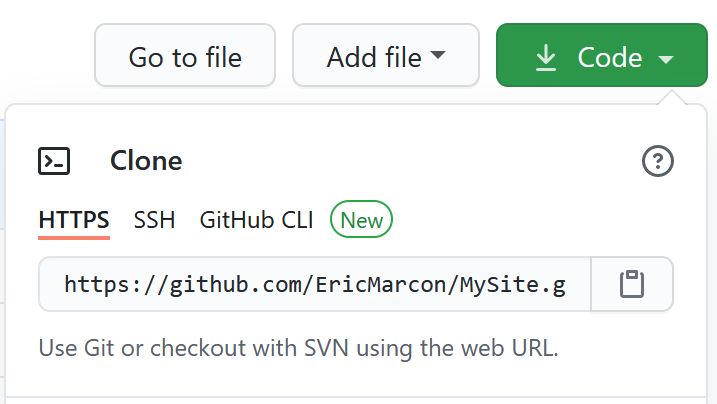
\includegraphics[width=0.8\linewidth]{images/rediger-GitHub-Clone} 

}

\caption{Copie de l'adresse d'un dépôt à cloner sur GitHub.}\label{fig:rediger-GitHub-Clone}
\end{figure}

\normalsize

Dans RStudio, créer un nouveau projet à partir de GitHub: dans le menu des projets en haut à droite, cliquer sur \enquote{New Project\ldots{}} puis \enquote{Version Control} puis \enquote{Git} puis coller l'adresse dans le champ \enquote{Repository URL} (figure \ref{fig:rediger-Projet-GitHub}).
Sélectionner le dossier dans lequel le projet sera créé en cliquant sur \enquote{Browse} et enfin cliquer sur \enquote{Create Project}.



\scriptsize

\begin{figure}

{\centering 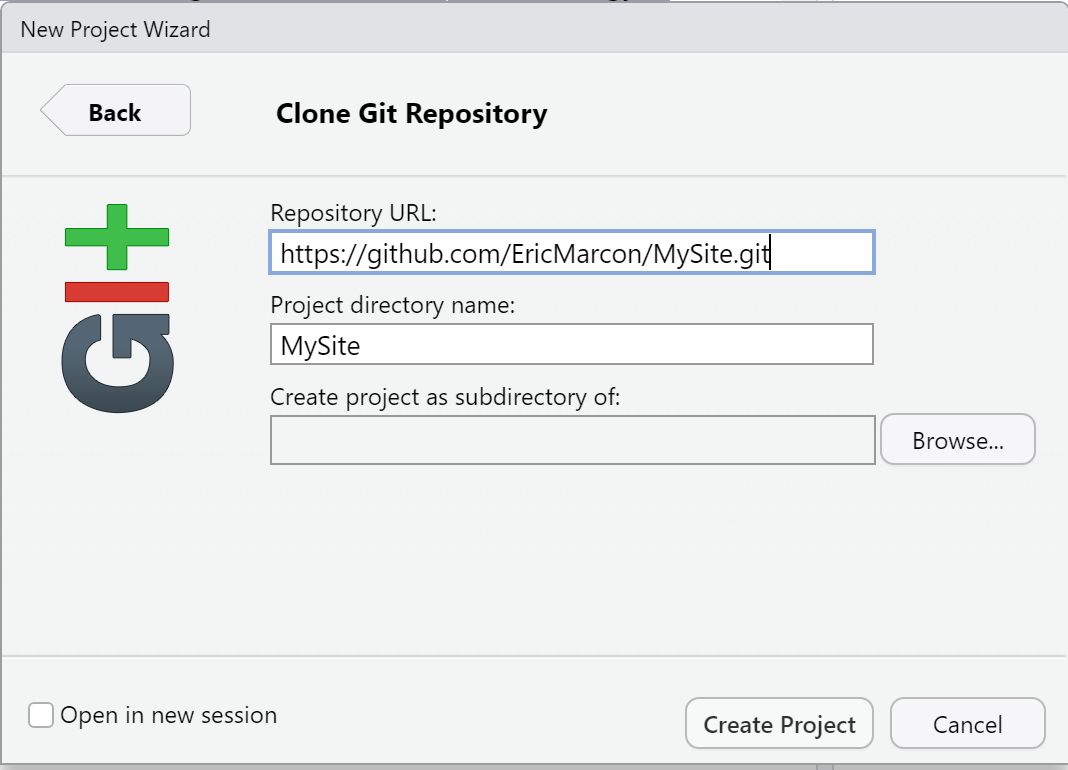
\includegraphics[width=0.8\linewidth]{images/rediger-Projet-GitHub} 

}

\caption{Collage de l'adresse du dépôt à cloner.}\label{fig:rediger-Projet-GitHub}
\end{figure}

\normalsize

Le projet créé est une copie exacte du modèle, qui doit être personnalisée.

RStudio ajoute automatiquement à la fin du fichier \texttt{.gitignore} une ligne pour ignorer ses fichiers de travail (dossier \texttt{.Rproj.user}).
Ajouter une ligne de commentaire pour le signaler.
Le contenu de \texttt{.gitignore} doit être le suivant:

\begin{verbatim}
# R
.Rbuildignore
.RData
.Rhistory
.Rprofile
.Rproj.user

# Hugo
/resources/
/public/

# blogdown
/static/en/
/static/fr/
*.rmarkdown
_index.html
index.html
**/index_files/
\end{verbatim}

Un bug de \textbf{blogdown} nécessite de déplacer le fichier \texttt{config.toml} du dossier \texttt{config/\_default/} à la racine du projet.

Prendre en compte ces modification dans git en faisant un commit.

\subsection{Construction du site}\label{construction-du-site}

Exécuter

\scriptsize

\begin{Shaded}
\begin{Highlighting}[]
\NormalTok{blogdown}\SpecialCharTok{::}\FunctionTok{build\_site}\NormalTok{(}\AttributeTok{build\_rmd =} \ConstantTok{TRUE}\NormalTok{)}
\end{Highlighting}
\end{Shaded}

\normalsize

pour construire le site web, y compris ses futures pages R Markdown.

Pour afficher le site, exécuter:

\scriptsize

\begin{Shaded}
\begin{Highlighting}[]
\NormalTok{blogdown}\SpecialCharTok{:::}\FunctionTok{serve\_site}\NormalTok{()}
\end{Highlighting}
\end{Shaded}

\normalsize

Il apparaît dans la fenêtre \emph{Viewer} de RStudio, dont le bouton d'agrandissement permet l'affichage dans le navigateur internet par défaut du système.

Pour modifier le contenu du site, il est préférable d'arrêter le serveur web par la commande:

\scriptsize

\begin{Shaded}
\begin{Highlighting}[]
\NormalTok{blogdown}\SpecialCharTok{:::}\FunctionTok{stop\_server}\NormalTok{()}
\end{Highlighting}
\end{Shaded}

\normalsize

Le site produit par \textbf{blogdown} se trouve dans le dossier \texttt{public} qui peut être copié directement sur un serveur web qui l'hébergera.
Une solution simple consiste à déclarer ce dossier comme racine des pages GitHub du projet
(section \ref{sec:github-pages}).
La méthode optimale consiste à utiliser l'intégration continue (voir section \ref{sec:blogdown-ci}) pour le copier à la racine de la branche \texttt{gh-pages} qui sera déclarée comme emplacement du site sur GitHub.

\subsection{Site multilingue}\label{site-multilingue}

Si le site est multilingue, son contenu (dossier \texttt{content}) doit être copié dans un dossier correspondant à chaque langue.
Par exemple, le fichier \texttt{content/authors/admin/\_index.md} qui contient les informations sur le propriétaire du site est remplacé par \texttt{content/en/authors/admin/\_index.md} et \texttt{content/fr/authors/admin}\break\texttt{/\_index.md} si le site supporte l'Anglais et le Français.
En pratique, créer un dossier \texttt{en} et un dossier \texttt{fr} dans \texttt{content}.
Déplacer tout le contenu de original de \texttt{content} dans \texttt{en} puis copier ce même contenu dans \texttt{fr}.

\subsection{Paramétrer}\label{paramuxe9trer}

Les fichiers de configuration du site sont bien documentés et offrent de nombreuses options.
Les principales sont passées en revue ici pour une création rapide d'un site fonctionnel.

Le fichier \texttt{config.toml} contient les paramètres généraux du site.
Les lignes à mettre à jour sont celle du titre du site (le nom du propriétaire puisqu'il s'agit d'un site personnel) et son adresse publique.
Pour le site exemple:

\begin{verbatim}
title = "Eric Marcon"
baseurl = "https://EricMarcon.github.io/"
\end{verbatim}

Il contient aussi la ligne de sélection de la langue par défaut (\enquote{en} ou \enquote{fr} au choix) et celle qui permet de placer les fichiers produits par Hugo dans chaque dossier de langue (\enquote{true} obligatoirement pour un site multilingue):

\begin{verbatim}
defaultContentLanguage = "fr"
defaultContentLanguageInSubdir = true
\end{verbatim}

Le dossier \texttt{config/\_default/} contient les autres fichiers de configuration.

\texttt{languages.toml} contient les paramètres linguistiques et les traductions de menus.
Pour chaque langue, la version utilisée et le dossier de contenu sont précisés:

\begin{verbatim}
[en]
  languageCode = "en-us"
  contentDir = "content/en"
[fr]
  languageCode = "fr-fr"
  contentDir = "content/fr"
\end{verbatim}

Pour les langues additionnelles, le titre du site, les paramètres d'affichage des dates et la traduction des menus sont ajoutés.
Dans la section \texttt{{[}fr{]}}:

\begin{verbatim}
[fr]
  languageCode = "fr-fr"
  contentDir = "content/fr"
  title = "Eric Marcon"
  description = "Page personnelle d'Eric Marcon"
  [fr.params]
    description = ""
    date_format = "02-Jan-2006"
    time_format = "15:04"
  [[fr.menu.main]]
    name = "Accueil"
    url = "#about"
    weight = 20
(...)
\end{verbatim}

Ces lignes sont commentées dans le modèle et doivent dont être décommentées en retirant les \texttt{\#} en têtes de lignes.

Les menus sont décrits plus bas.

\texttt{params.toml} décrit l'aspect du site.
Les options sont regroupées par sujet, par exemple \enquote{Theme} pour l'apparence générale.
Dans \enquote{Basic Info}, la ligne

\begin{verbatim}
site_type = "Person"
\end{verbatim}

sélectionne un site personnel.
Il est possible d'utiliser Academic pour un site de projet scientifique ou un site d'unité, non documentés en détail ici.
Les principales différences sont, pour un site collectif:

\begin{itemize}
\tightlist
\item
  la gestion des auteurs: dans le dossier \texttt{/contents/\textless{}langue\textgreater{}/authors}, un seul dossier \texttt{admin} est utilisé pour un site personnel alors qu'un dossier par personne est nécessaire pour un site collectif;
\item
  un composant décrit plus bas, qui permet de présenter les personnes, doit être activé.
\end{itemize}

La description du site dans la langue par défaut est saisie, à destination des moteurs de recherche:

\begin{verbatim}
description = "Eric Marcon's Homepage"
\end{verbatim}

Elle doit être traduite dans le fichier \texttt{languages.toml}, dans chaque langue.

Dans \enquote{Site Features}, nous sélectionnons la coloration du code R, l'activation du formatage des équations et l'avertissement légal pour l'utilisation des cookies.

\begin{verbatim}
highlight_languages = ["r"] 
math = true
privacy_pack = true
\end{verbatim}

La ligne \texttt{edit\_page} doit être mise à jour: remplacer le dépôt par défaut \enquote{\url{https://github.com/gcushen/hugo-academic}} par celui du site.

\enquote{Contact details} contient les informations pour contacter le propriétaire du site.
Elles doivent être saisies.

\enquote{Regional Settings} contient les paramètres d'affichage de date pour la langue par défaut (ceux des autres langues sont dans \texttt{languages.toml}).
Ils n'ont normalement pas à être modifiés.

\enquote{Comments} permet d'activer les commentaires des visiteurs en bas de pages, avec Disqus ou Comment.io (un compte est nécessaire chez le fournisseur).
\enquote{Marketing} permet d'activer le suivi de fréquentation du site en saisissant simplement son identifiant Google Analytics (à créer avec un compte Google).
\enquote{Content Management System} contient la ligne \texttt{netlify\_cms} dont la valeur doit être \texttt{false} si le site n'est pas hébergé par Netlify.
Enfin \enquote{Icon Pack Extensions} permet d'activer les icônes Academicons si nécessaire.

\subsection{Ecrire}\label{ecrire-3}

Utiliser la documentation en ligne\footnote{\url{https://wowchemy.com/docs/page-builder/}} en complément des informations principales détaillées ici.
L'exemple utilisé ici est le site personnel de l'auteur\footnote{\url{https://EricMarcon.github.io/}}.

La méthode de travail consiste à progresser pas à pas en testant puis validant chaque étape:

\begin{itemize}
\tightlist
\item
  effectuer les modifications;
\item
  construire le site et vérifier le résultat: \texttt{blogdown:::serve\_site()};
\item
  arrêter le site: \texttt{blogdown::stop\_server()};
\item
  si le résultat n'est pas satisfaisant, recommencer;
\item
  valider les modifications (\emph{commit}).
\end{itemize}

\subsubsection{Page d'accueil}\label{page-daccueil}

La page d'accueil du site est constituée par une suite d'éléments (\emph{widgets}) qui se trouvent dans \texttt{/contents/\textless{}langue\textgreater{}/home}.
Chaque élément est décrit par un fichier markdown.
Le premier est \texttt{index.md}.
Il n'est normalement jamais modifié.
Son contenu est le suivant:

\begin{verbatim}
+++
# Homepage
type = "widget_page"
headless = true  # Homepage is headless, other widget 
pages are not.
+++
\end{verbatim}

Le fichier ne contient qu'un entête au format TOML, encadré par une ligne de \texttt{+++}.
Le type de composant (\texttt{type}) indique qu'il s'agit d'une page de composants, dans laquelle les autres composants du dossier trouveront leur place.
\texttt{headless\ =\ true} signifie que la page n'a pas d'en-tête.



\scriptsize

\begin{figure}

{\centering 
\includegraphics[width=0.8\linewidth]{images/rediger-demo} 

}

\caption{Composant \texttt{demo} dans Academic.}\label{fig:rediger-demo}
\end{figure}

\normalsize

Le composant \texttt{demo.md} (figure \ref{fig:rediger-demo}) est un composant de type \enquote{blank}, c'est-à-dire une page de texte libre: il sert ici à présenter le modèle Academic Kickstart et doit donc être désactivé.
L'entête contient ses informations de formatage (titre, nombre de colonnes, couleurs\ldots) et le contenu de la page est écrit en markdown.
Les composants apparaissent par ordre croissant de poids (\texttt{weight} dans l'entête): 15 marque le premier composant dans le modèle Academic.
Le composant peut être désactivé en supprimant son fichier ou en modifiant sa propriété \texttt{active} dans l'entête:

\begin{verbatim}
active = false  # Activate this widget? true/false
\end{verbatim}



\scriptsize

\begin{figure}

{\centering 
\includegraphics[width=0.8\linewidth]{images/rediger-about} 

}

\caption{Composant \texttt{about} dans Academic.}\label{fig:rediger-about}
\end{figure}

\normalsize

Le composant suivant est \texttt{about.md} (figure \ref{fig:rediger-about}).
Il présente le propriétaire du site.
Son titre doit être localisé.
Dans le dossier \texttt{/content/fr/home}, sa valeur sera:

\begin{verbatim}
title = "Biographie"
\end{verbatim}

L'auteur (\texttt{author}) doit correspondre à un dossier de \texttt{/contents/\textless{}langue\textgreater{}}\break\texttt{/authors}.
\texttt{admin} convient parfaitement pour un site personnel.
Academic permet de créer des sites d'équipes: dans cette configuration, un dossier par personne serait nécessaire.
L'image affichée par le composant est le fichier \texttt{avatar.jpg} placé dans ce dossier.
Limiter la taille du fichier pour la performance du site (moins d'un mégaoctet est une taille raisonnable), tout en assurant une taille minimale de quelques centaines de pixels de côté pour la qualité de l'affichage.

Le contenu du composant est lu dans le fichier \texttt{\_index.md} du même dossier, qui contient toutes les informations sur l'auteur.
Son organisation est assez claire: modifier son contenu à partir de l'exemple fourni.
Si des icônes de type \texttt{ai} sont utilisées, activer le pack d'icône Academicons dans \texttt{config/\_default/params.toml}.



\scriptsize

\begin{figure}

{\centering 
\includegraphics[width=0.8\linewidth]{images/rediger-skills} 

}

\caption{Composant \texttt{skills} dans Academic.}\label{fig:rediger-skills}
\end{figure}

\normalsize

Le composant talents (\texttt{skills}, figure \ref{fig:rediger-skills}) présente les compétences de l'auteur de façon graphique.
Une collection d'icônes est disponible, et des icônes nouvelles peuvent être ajoutées.



\scriptsize

\begin{figure}

{\centering 
\includegraphics[width=0.8\linewidth]{images/rediger-experience} 

}

\caption{Composant \texttt{experience} dans Academic.}\label{fig:rediger-experience}
\end{figure}

\normalsize

Le composant expérience (\texttt{experience}, figure \ref{fig:rediger-experience}) liste les expériences professionnelles.
Toutes les informations sont saisies dans son entête.

Le composant \texttt{accomplishments} présente les formations professionnelles et permet d'accéder à leurs certificats.

Le composant \texttt{posts} va chercher son contenu dans le dossier \texttt{/contents}\break\texttt{/\textless{}langue\textgreater{}/post} qui contient les billets de blog (voir plus bas).
Le fichier \texttt{posts.md} contient des options de mise en page dans son entête.

Le composant \texttt{projects} fonctionne de la même façon.
La différence entre les deux composants est leur mise en forme: \texttt{posts} est du type \enquote{pages}, qui affiche les éléments les plus récents, alors que \texttt{projects} est de type \enquote{portfolio}, qui affiche les éléments sélectionnés qui contiennent la description \texttt{featured:\ true} dans leur propre entête.
Il est possible de créer des composants de ces types librement, en spécifiant le dossier contenant les éléments dans \enquote{page-type}.
Exemple: créer un composant nommé \texttt{software.md} en renommant \texttt{projects.md}, modifier sa ligne \texttt{page\_type\ =\ "software"} et créer un dossier \texttt{/contents/\textless{}langue\textgreater{}/software} pour y placer du contenu.

Les composants \texttt{publications} et \texttt{featured} sont de type \enquote{pages} et \enquote{portfolio} respectivement et prennent leur contenu dans le dossier \texttt{publication}.

Le composant \texttt{tags} présente un nuage de mots à partir des mots-clés déclarés dans tous les fichiers de contenu (billets de blog, publications\ldots) sous la forme suivante dans leur entête:

\begin{verbatim}
tags = ["Mot Clé 1", "Autre Mot Clé"]
\end{verbatim}

Enfin, le composant \texttt{contact} permet d'afficher un formulaire de contact.
Il utilise les informations du fichier \texttt{config/\_default/params.toml} dans sa partie commençant par:

\begin{verbatim}
############################
## Contact details
##
\end{verbatim}

Pour afficher une carte, entrer la latitude et la longitude de l'adresse dans la ligne \texttt{coordinates}.
Pour afficher un formulaire de messagerie, choisir le service \emph{formspree.io} (\texttt{email\_form\ =\ 2} dans \texttt{contact.md}).
Pour activer le service de messagerie, il faudra construire le site web, s'envoyer un premier message en utilisant le formulaire et suivre les instructions de Formspree.

Le composant \texttt{people} est utilisé dans les sites collectifs pour présenter les membres.
Le composant \texttt{slider} permet d'afficher un carrousel (des éléments défilants) en haut de page.
Pour comprendre son fonctionnement, le plus simple consiste à l'activer.

\subsubsection{Menu de la page d'accueil}\label{menu-de-la-page-daccueil}

La page d'accueil comporte un menu qui permet de naviguer rapidement vers ses composants ou vers d'autres pages.
Il est paramétré dans \texttt{config/\_default}\break\texttt{/menus.toml}.
Les éléments du menu ont un nom affiché, un lien (commençant par \texttt{\#} pour pointer vers un composant ou un chemin relatif dans le site comme \texttt{publication/}), et un poids qui définit leur ordre d'affichage, de la même façon que celui des composants de la page d'accueil.

Un menu à deux éléments pour pointer vers l'accueil du site et les billets de blogs est donc le suivant:

\begin{verbatim}
[[main]]
  name = "Home"
  url = "#about"
  weight = 10

[[main]]
  name = "Posts"
  url = "#posts"
  weight = 20
\end{verbatim}

Le menu doit être traduit dans chaque langue dans le fichier \texttt{config/\_default}\break\texttt{/languages.toml}:

\begin{verbatim}
[fr]
  [[fr.menu.main]]
    name = "Accueil"
    url = "#about"
    weight = 10
  [[fr.menu.main]]
    name = "Articles"
    url = "#posts"
    weight = 20
\end{verbatim}

\subsubsection{Billets}\label{billets}

Le site est alimenté par des billets de blog placés dans le dossier \texttt{/contents/\textless{}langue\textgreater{}/post}.
Il doivent être traduits et placés dans le dossier \texttt{post} de chaque langue pour être disponibles dans la langue correspondante.
L'exemple utilisé ici est un guide pour estimer correctement la densité d'une variable bornée\footnote{\url{https://EricMarcon.github.io/post/densite/}}.

Son code est sur GitHub\footnote{\url{https://github.com/EricMarcon/HomePage2020/tree/master/content/fr/post/densite}}.

Un billet est placé dans un dossier (\texttt{/content/fr/post/densite}) qui contient son code R Markdown et éventuellement des images, des données pour alimenter le code et d'autres éléments appelés par le code.
Hugo supporte des fichiers markdown natifs.
L'apport de \textbf{blogdown} relativement à un site Hugo natif est le support de R Markdown, donc la possibilité d'exécuter tout code R comme dans un bloc-note (dont le contenu peut être réutilisé sans modification).

Le fichier principal d'un billet est \texttt{index.Rmd}.
\textbf{blogdown} crée un fichier \texttt{index.html} pendant la construction du site: il peut être ignoré (dans \texttt{.gitgnore}) et supprimé à tout moment.
Si une image \texttt{featured.png} (optimale pour un schéma) ou \texttt{featured.jpg} (optimale pour un photo) est placée dans le dossier, elle sera utilisée comme vignette du billet.

\texttt{index.Rmd} comprend un entête au format yaml (entourée par des \texttt{-\/-\/-}) ou toml (entourée par des \texttt{+++}) qui décrit son affichage:

\begin{verbatim}
---
title: "Titre du billet"
subtitle: "Sous-titre"
summary: "Résumé"
authors: []
tags: ["Mot Clé 1", "Autre Mot Clé"]
categories: []
date: 2020-04-17
featured: false
draft: false

# Featured image
# To use, add an image named `featured.jpg/png` to 
# your page's folder.
# Focal points: Smart, Center, TopLeft, Top, TopRight,
# Left, Right, BottomLeft, Bottom, BottomRight.
image:
  caption: ""
  focal_point: ""
  preview_only: false
  
bibliography: references.bib
---
\end{verbatim}

Les auteurs sont utilisés dans les sites collectifs.
Les tags permettent d'alimenter le composant nuage de mots s'il est activé dans la page d'accueil.
Les catégories permettent de rechercher des pages au contenu similaire (recherche par mot-clé sur le site).
L'option \texttt{featured:\ true} fait apparaître le billet dans les composants de type \texttt{featured} sur la page d'accueil.
L'option \texttt{draft:\ true} cache le billet.

Les éléments suivants précisent l'affichage de la vignette: légende et position.
L'option \texttt{preview\_only:\ true} limite l'affichage aux miniatures (sur la page d'accueil), retirant donc l'image du billet lui-même.

Les éléments d'entête nécessaires au corps de texte R Markdown, comme le nom du fichier contenant les références bibliographiques, placé dans le même dossier, sont ajoutés.

Le corps du texte est celui d'un document R Markdown standard, avec du code R inclus.
Un bout de code initial permet de fixer les options de R et charger les packages nécessaires.

En pratique, la façon la plus efficace de créer un nouveau billet est de copier le dossier complet d'un billet précédent, de le renommer et de modifier son contenu.
La commande \texttt{blogdown::new\_post()} peut aussi être utilisée mais ne gère pas les langues multiples (et crée donc le billet dans le dossier \texttt{/contents/post} à moins de préciser l'argument \texttt{subdir}).

La reconstruction du site ne met par défaut pas à jour les pages basées sur un fichier \texttt{.Rmd}.
Pour le faire, il faut forcer la commande \texttt{build\_site()}.

\scriptsize

\begin{Shaded}
\begin{Highlighting}[]
\NormalTok{blogdown}\SpecialCharTok{::}\FunctionTok{build\_site}\NormalTok{(}\AttributeTok{build\_rmd =} \ConstantTok{TRUE}\NormalTok{)}
\NormalTok{blogdown}\SpecialCharTok{::}\FunctionTok{serve\_site}\NormalTok{()}
\end{Highlighting}
\end{Shaded}

\normalsize

\subsubsection{Publications}\label{publications}

Les publications sont organisées comme les billets, mais placées dans le dossier \texttt{/contents/\textless{}langue\textgreater{}/publications}.

L'exemple utilisé est un article de revue\footnote{\url{https://EricMarcon.github.io/publication/marcon-2003-a/}} avec son code\footnote{\url{https://github.com/EricMarcon/HomePage2020/tree/master/content/fr/publication/marcon-2003-a}}.

Un fichier \texttt{cite.bib} contenant la référence au format BibTeX est placé dans le dossier.
Le nom du dossier est de préférence celui de l'identifiant de la publication.
L'entête du fichier \texttt{index.md} (ici au format Markdown, mais \texttt{.Rmd} est possible si du code R est nécessaire) contient les mêmes informations que le fichier BibTeX, mais au format approprié (yaml), et les éléments propres à Academic (\texttt{featured}):

\begin{verbatim}
---
title: "Evaluating the geographic concentration of |>
industries using distance-based methods"
authors: ["Eric Marcon", "Florence Puech"]
publication_types: ["2"]
abstract: "We propose (...)"
publication: "*Journal of Economic Geography*"
doi: "10.1093/jeg/lbg016"

date: 2003-10-01
featured: false
---
\end{verbatim}

Les types de publication sont:

\begin{itemize}
\tightlist
\item
  0 = Uncategorized;
\item
  1 = Conference paper;
\item
  2 = Journal article;
\item
  3 = Preprint / Working Paper;
\item
  4 = Report;
\item
  5 = Book;
\item
  6 = Book section;
\item
  7 = Thesis;
\item
  8 = Patent.
\end{itemize}

Des boutons sont affichés en haut de la page de la publication en fonction des informations trouvées:

\begin{itemize}
\tightlist
\item
  PDF: si la ligne \texttt{url} est présente dans l'en-tête;
\item
  Citation: si le fichier \texttt{cite.bib} est présent dans le dossier;
\item
  DOI: si la ligne \texttt{doi} est présente dans l'en-tête.
\end{itemize}

Le corps de la publication contient un lien (au format HTML) vers le site Dimension qui fournit des informations bibliométriques.
Ce lien peut être réutilisé très simplement, en remplaçant simplement le DOI du document:

\begin{verbatim}
<span class="__dimensions_badge_embed__" 
  data-doi="10.1093/jeg/lbg016"></span>
<script async src="https://badge.dimensions.ai/
  badge.js" charset="utf-8"></script>
\end{verbatim}

Enfin, un fichier \texttt{/contents/\textless{}langue\textgreater{}/publications/\_index.Rmd} permet de présenter la bibliographie complète.
Il est accessible à partir du composant \texttt{publications} de la page d'accueil qui affiche un lien \enquote{Plus de Publications}.

Le fichier exemple\footnote{\url{https://EricMarcon.github.io/publication/}} avec son code\footnote{\url{https://github.com/EricMarcon/HomePage2020/tree/master/content/fr/publication/marcon-2003-a}} permet d'interroger Google Scholar pour obtenir le réseau de coauteurs, l'indice h et le nombre de citations annuelles de l'auteur.
Il est réutilisable en modifiant simplement l'identifiant Google Scholar à la ligne 30.

En faisant exécuter le code régulièrement, par exemple par GitHub (voir ci-dessous), les statistiques affichées sont maintenues à jour sans intervention humaine.

\subsubsection{Communications}\label{communications}

Les communications sont organisées comme les publications, dans le dossier \texttt{/contents/\textless{}langue\textgreater{}/talk}.

L'exemple utilisé est une communication en Français, donc dans \texttt{/contents/fr/talk}\footnote{\url{https://EricMarcon.github.io/talk/chao1/}} avec son code\footnote{\url{https://github.com/EricMarcon/HomePage2020/tree/master/content/fr/talk/chao1}}.

Une image peut être utilisée plus facilement que pour une publication.

L'entête contient des lignes particulières adaptées aux communications:

\begin{verbatim}
---
title: "Construction de l'estimateur de biodiversité |>
Chao1"
event: "Semaine des mathématiques 2020"
event_url: https://eduscol.education.fr/cid59178/|>
semaine-des-mathematiques.html

location: Université de Guyane

summary: []
abstract: |
  Pour estimer le nombre d’espèces (richesse 
  spécifique) d’une communauté à partir d’un 
  échantillon, l’estimateur Chao1 est l’outil 
  le plus utilisé.

  Sa construction est expliquée et son efficacité
  est testée sur des données simulées.

# Talk start and end times.
#   End time can optionally be hidden by 
# prefixing the line with `#`.
date: "2020-03-11T11:00:00Z"
date_end: "2020-03-11T12:00:00Z"
all_day: false

# Schedule page publish date (NOT talk date).
publishDate: "2020-04-14"

# Is this a featured talk? (true/false)
featured: false

image:
  caption: 'Produit scalaire des vecteurs $v_0$ |>
et $v_2$'
  focal_point: Smart

url_code: "https://github.com/EricMarcon/Chao1"
url_pdf: "https://EricMarcon.github.io/Chao1/|>
Chao1.pdf"
url_slides: "https://EricMarcon.github.io/Chao1/|>
Chao1.html"

# Enable math on this page?
math: true
---
\end{verbatim}

Les liens (\texttt{url\_code} par exemple) font apparaître des boutons qui permettent d'afficher respectivement le code source de la présentation, un fichier pdf et les diapositives en ligne.

\subsubsection{Autres éléments}\label{autres-uxe9luxe9ments}

Il est possible d'ajouter librement des éléments supplémentaires sur le site:

\begin{itemize}
\tightlist
\item
  dans \texttt{/contents/\textless{}langue\textgreater{}/}, créer un dossier dont le nom est le type d'éléments (exemple: \texttt{recette});
\item
  ajouter des éléments dans ce dossier, chacun dans son propre dossier;
\item
  le fichier obligatoire est \texttt{index.md} ou \texttt{index.Rmd} avec un en-tête contenant possiblement tous les champs rencontrés dans les éléments \texttt{post}, \texttt{publication} et \texttt{talk};
\item
  le fichier de vignette, \texttt{featured.png} ou \texttt{featured.jpg}, est facultatif;
\item
  tous les fichiers nécessaires au tricot (images, données) peuvent être ajoutés dans le même dossier;
\item
  dans \texttt{/contents/\textless{}langue\textgreater{}/home}, ajouter un composant de la page d'accueil en copiant-collant un élément existant de type \enquote{pages} (comme \texttt{publications}) ou \enquote{portfolio} (comme \texttt{featured}) et le paramétrer pour qu'il pointe sur le bon dossier (dans l'exemple: \texttt{page-type=recette}) et ajuster son apparence (nombre d'éléments par exemple) et sa position (poids);
\item
  ajouter éventuellement une entrée de menu pour pointer sur le composant, avec le même poids que le composant.
\end{itemize}

Les fichiers d'index peuvent porter l'extension \texttt{.Rmd} ou \texttt{.md}.
Dans le premier cas, ils seront traités par \textbf{blogdown}, qui supporte l'intégration de code R.
Dans l'autre cas, ils seront traités par Hugo, qui ne gère que le format markdown standard.
Les fichiers \texttt{.md} nécessitent moins de ressource et sont donc préférés quand ils suffisent.

\subsubsection{Finitions}\label{finitions-1}

L'icône du site, qui apparaît dans la barre d'adresse des navigateurs web, se trouve dans \texttt{assets/images}.
Le fichier \texttt{icon.png} peut être remplacé.

\subsection{Intégration continue}\label{sec:rediger-web-ci}

La construction du site web en production peut être confiée à GitHub (section \ref{sec:blogdown-ci}), y compris sa mise à jour périodique si des pages du site traitent des données qui évoluent dans le temps.

\subsection{Mises à jour}\label{mises-uxe0-jour-1}

Le thème Academic est régulièrement mis à jour.
La version utilisée est indiquée dans le fichier \texttt{go.mod}.
Pour utiliser la dernière version officielle, exécuter dans la console R la commande suivante:

\scriptsize

\begin{Shaded}
\begin{Highlighting}[]
\NormalTok{blogdown}\SpecialCharTok{::}\FunctionTok{hugo\_cmd}\NormalTok{(}\StringTok{"mod get {-}u"}\NormalTok{)}
\end{Highlighting}
\end{Shaded}

\normalsize

Les fichiers \texttt{go.mod} et \texttt{go.sum}, qui contient les codes de hachage des fichiers du module, sont mis à jour.

Chaque changement de version peut nécessiter des adaptations du contenu du site, référencées dans la documentation en ligne du thème\footnote{\url{https://wowchemy.com/updates/}}.

Mettre Hugo à jour en même temps:

\scriptsize

\begin{Shaded}
\begin{Highlighting}[]
\NormalTok{blogdown}\SpecialCharTok{::}\FunctionTok{update\_hugo}\NormalTok{()}
\end{Highlighting}
\end{Shaded}

\normalsize

\section{Exportation de figures}\label{exportation-de-figures}

Quand la production de documents avec R Markdown n'est pas possible, les figures issues de R doivent être exportées sous forme de fichiers pour être intégrés dans un autre processus d'écriture.
Il est préférable de créer des scripts pour créer les figures de façon reproductible et au format optimal.

\subsection{Formats vectoriels et raster}\label{formats-vectoriels-et-raster}

Les figures doivent en général être produites dans un format vectoriel:

\begin{itemize}
\tightlist
\item
  SVG pour la publication d'affiches ou de posters;
\item
  EMF (Extended Meta-File) pour Word ou la suite Microsoft Office qui ne supporte pas d'autres formats;
\item
  EPS (Encapsulated PostScript) ou PDF (Portable Document Format) pour LaTeX.
\end{itemize}

Les figures raster (composées d'un ensemble de points, comme les photographies) sont rares dans R.
La fonction \texttt{image()} utilisée pour afficher des cartes utilise par défaut des polygones plutôt que des points.
La figure \ref{fig:volcano} montre le résultat du code suivant:



\scriptsize

\begin{figure}

{\centering 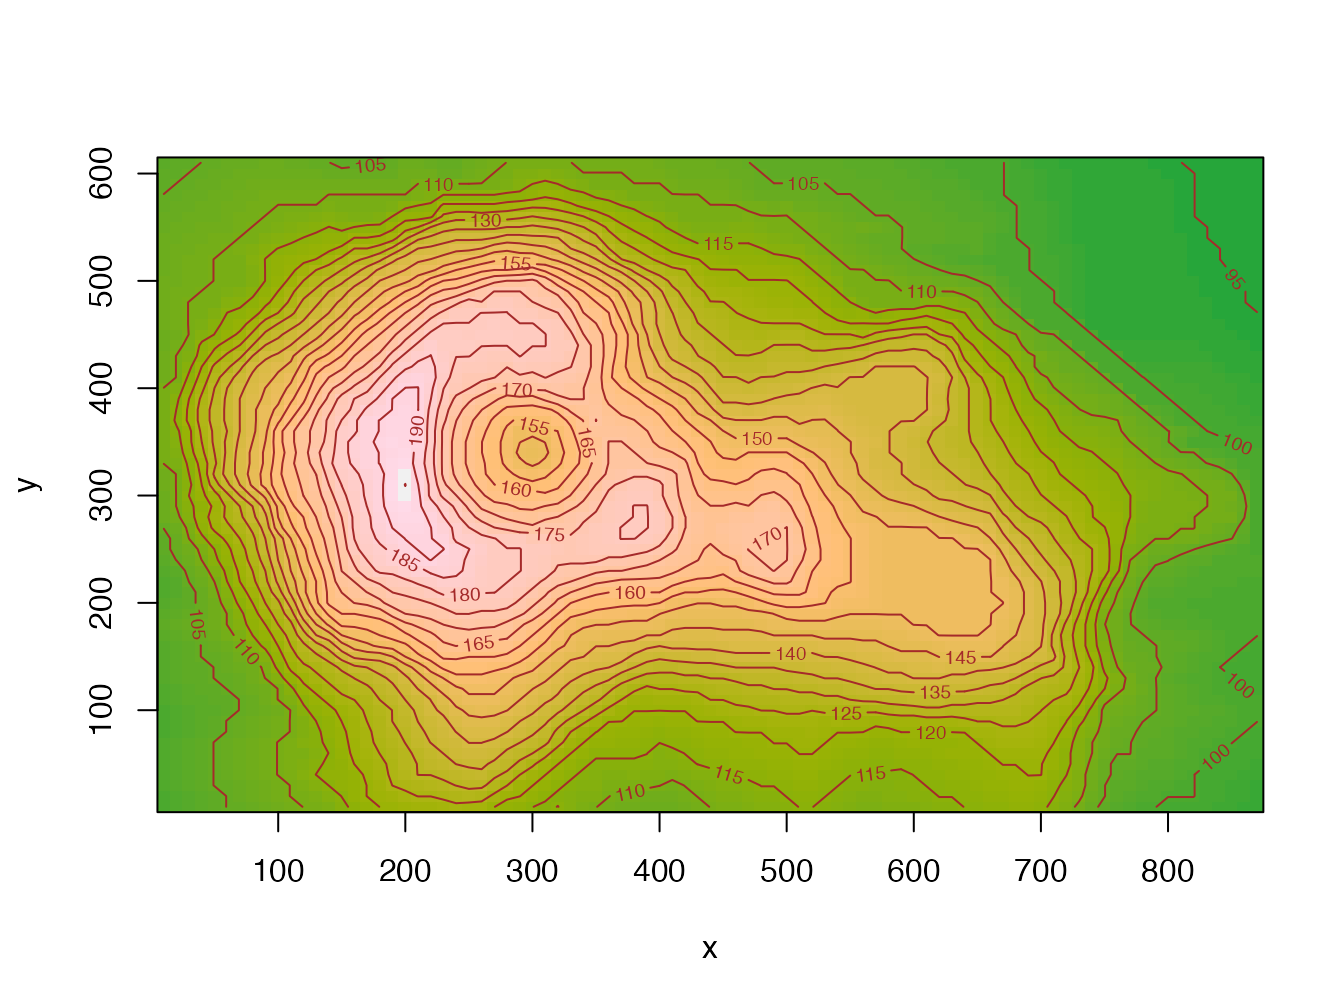
\includegraphics[width=0.8\linewidth]{travailleR_files/figure-latex/volcano-1} 

}

\caption{Courbes de niveau du volcan Maunga Whau, code fourni en exemple de l'aide de la fonction \texttt{image()}.}\label{fig:volcano}
\end{figure}

\normalsize

Elle est composée d'un ensemble de rectangles colorés: il s'agit bien d'une image vectorielle.

Si nécessaire, des images peuvent être produites aux formats BMP (bitmap, sans compression), JPEG (compressées avec perte de qualité), PNG (compressées sans perte de qualité, avec transparence possible) ou Tiff (compressées ou non).

\subsection{Fonctions}\label{fonctions}

Les graphiques produits par \texttt{ggplot()} peuvent être sauvegardés dans un fichier par la fonction \texttt{ggsave()}.
L'extension du nom du fichier définit son format.
Voir l'aide de la fonction pour plus de détails.

Les autres graphiques nécessitent une méthode différente.
La fonction \texttt{postscript()} produit un fichier EPS.
Le code R doit appeler la fonction pour créer le fichier, produire la figure, puis fermer le fichier, par exemple:

\scriptsize

\begin{Shaded}
\begin{Highlighting}[]
\CommentTok{\# Ouverture du fichier}
\FunctionTok{postscript}\NormalTok{(}\StringTok{"Fig1.eps"}\NormalTok{, }\AttributeTok{width =} \DecValTok{6}\NormalTok{, }\AttributeTok{height =} \DecValTok{4}\NormalTok{, }\AttributeTok{horizontal =} \ConstantTok{FALSE}\NormalTok{)}
\CommentTok{\# Création de la figure}
\FunctionTok{plot}\NormalTok{(cars)}
\CommentTok{\# Fermeture du fichier}
\FunctionTok{dev.off}\NormalTok{()}
\end{Highlighting}
\end{Shaded}

\begin{verbatim}
## pdf 
##   2
\end{verbatim}

\normalsize

La largeur et la hauteur (en pouces) d'un fichier vectoriel n'ont pas d'importance, mais leur rapport fixe l'aspect de la figure.
La taille des textes est fixe: augmenter la taille de la figure revient donc à diminuer la taille relative des textes: procéder par essais successifs, en veillant à ce que les légendes restent lisibles à la taille finale de la figure.

L'argument \texttt{horizontal} fixe l'orientation de la figure de façon assez imprévisible: procéder par essais.

Les fonctions \texttt{eps()}, \texttt{pdf()}, \texttt{bmp()}, \texttt{jpeg()}, \texttt{png()} et \texttt{tiff()} fonctionnent de la même manière.
Se référer à l'aide des fonctions pour le choix des options (résolution, niveau de compression, etc.).
La fonction \texttt{emf()} est fournie par le package \textbf{devEMF}.

Les polices de caractères ne sont pas incluses dans les fichiers EPS ou PDF.
Si nécessaire, la fonction \texttt{embedFonts()} permet d'y remédier, à condition que GhostScript soit installé.

\subsection{Package ragg}\label{package-ragg}

Le package \textbf{ragg}\footnote{\url{https://ragg.r-lib.org/}} améliore la qualité des fichiers PNG, JPEG et TIFF.
Les fonctions optimisées sont \texttt{agg\_png()}, \texttt{agg\_jpeg()}et \texttt{agg\_tiff()}. Leur usage est le même que celui des fonctions de \textbf{grDevices}.

Les documents R Markdown produisent des images au format PNG pour leur version HTML.
\textbf{ragg} améliore leur qualité: le package doit être installé et \texttt{dev\ =\ "ragg\_png"} doit être ajoutée aux options de \textbf{knitr}.
Pour ce document, les options déclarées dans \texttt{index.Rmd} sont les suivantes:

\scriptsize

\begin{Shaded}
\begin{Highlighting}[]
\CommentTok{\# knitr options}
\NormalTok{knitr}\SpecialCharTok{::}\NormalTok{opts\_chunk}\SpecialCharTok{$}\FunctionTok{set}\NormalTok{(}
  \AttributeTok{cache =}   \ConstantTok{FALSE}\NormalTok{,    }\CommentTok{\# Cache chunk results}
  \AttributeTok{include =} \ConstantTok{TRUE}\NormalTok{,     }\CommentTok{\# Show/Hide chunks}
  \AttributeTok{echo =}    \ConstantTok{TRUE}\NormalTok{,     }\CommentTok{\# Show/Hide code}
  \AttributeTok{warning =} \ConstantTok{FALSE}\NormalTok{,    }\CommentTok{\# Show/Hide warnings}
  \AttributeTok{message =} \ConstantTok{FALSE}\NormalTok{,    }\CommentTok{\# Show/Hide messages}
  \CommentTok{\# Figure alignment and size}
  \AttributeTok{fig.align =} \StringTok{\textquotesingle{}center\textquotesingle{}}\NormalTok{, }\AttributeTok{out.width =} \StringTok{\textquotesingle{}80\%\textquotesingle{}}\NormalTok{, }\AttributeTok{fig.asp =}\NormalTok{ .}\DecValTok{75}\NormalTok{,}
  \CommentTok{\# Graphic devices (ragg\_png is better than standard png)}
  \AttributeTok{dev =} \FunctionTok{c}\NormalTok{(}\StringTok{"ragg\_png"}\NormalTok{, }\StringTok{"pdf"}\NormalTok{),}
  \CommentTok{\# Code chunk format}
  \AttributeTok{tidy =} \ConstantTok{FALSE}\NormalTok{, }\AttributeTok{tidy.opts =} \FunctionTok{list}\NormalTok{(}\AttributeTok{blank =} \ConstantTok{FALSE}\NormalTok{, }\AttributeTok{width.cutoff =} \DecValTok{60}\NormalTok{),}
  \AttributeTok{size =} \StringTok{"scriptsize"}\NormalTok{, }\AttributeTok{knitr.graphics.auto\_pdf =} \ConstantTok{TRUE}
\NormalTok{  )}
\FunctionTok{options}\NormalTok{(}\AttributeTok{width =} \DecValTok{60}\NormalTok{)}
\end{Highlighting}
\end{Shaded}

\normalsize

Enfin, \textbf{ragg} peut être utilisé comme moteur de rendu graphique par défaut dans RStudio à partir de la version 1.4 (Menu \enquote{Tools \textgreater{} Global Options \textgreater{} General \textgreater{} Graphics \textgreater{} Backend}).

\section{Flux de travail}\label{sec:targetsmd}

Un flux de travail (voir section \ref{sec:targets}) peut être intégré dans un document R Markdown à partir de la version 0.5 du package \textbf{targets}.

\scriptsize

\begin{Shaded}
\begin{Highlighting}[]
\FunctionTok{library}\NormalTok{(}\StringTok{"targets"}\NormalTok{)}
\end{Highlighting}
\end{Shaded}

\normalsize

\subsection{Déclaration du flux}\label{duxe9claration-du-flux}

Le flux est géré par des bouts de code de type \texttt{targets}.
Leur entête minimal est \texttt{\{targets\}} au lieu de \texttt{\{r\}}, et ils doivent être nommés.
Ces bouts de code permettent de créer le fichier \texttt{\_targets.R} quand ils sont exécutés en mode non interactif, notamment pendant que le document est tricoté.
S'ils sont lancés en mode interactif, par exemple dans R Studio, leur code est exécuté.
L'option \texttt{tar\_interactive\ =\ FALSE} dans leur entête permet de les tester sans tricoter tout le document.

Un ancien flux éventuel doit être supprimé avant d'écrire le nouveau:

\scriptsize

\begin{Shaded}
\begin{Highlighting}[]
\FunctionTok{tar\_unscript}\NormalTok{()}
\end{Highlighting}
\end{Shaded}

\normalsize

Le premier bout de code, avec l'option \texttt{tar\_globals=TRUE}, écrit les options globales du flux.
Pour créer le flux présenté en section \ref{sec:targets}, le code est simplement:

\begin{verbatim}
```{targets targets_global, tar_globals=TRUE}
# Packages
tar_option_set(packages = c("spatstat", "dbmss"))
```
\end{verbatim}

Les fonctions utilisées par les cibles sont déclarées dans ce type de bout de code: elles sont ajoutées à un fichier dans le dossier de travail \texttt{\_targets\_r} (différent du dossier \texttt{\_targets} qui contient les fichiers de calcul des cibles).

\subsection{Déclaration des cibles}\label{duxe9claration-des-cibles}

Les cibles elles-mêmes sont déclarées dans des bouts de code dont le nom est celui de la variable de destination.

\begin{verbatim}
```{targets X, tar_simple=TRUE}
runifpoint(NbPoints)
```
\end{verbatim}

Chaque cible nécessite un bout de code construit de cette manière.
La valeur de la cible est la dernière valeur retournée, à la manière d'une fonction qui n'utiliserait pas \texttt{return()}.

Pendant le tricot, ce code simplifié (\texttt{tar\_simple=TRUE}) est transformé automatiquement en écriture de cible:

\scriptsize

\begin{Shaded}
\begin{Highlighting}[]
\FunctionTok{tar\_target}\NormalTok{(X, \{}
  \FunctionTok{runifpoint}\NormalTok{(NbPoints)}
\NormalTok{\})}
\end{Highlighting}
\end{Shaded}

\normalsize

La lecture du document est alourdie par cette syntaxe particulière: \textbf{targets} n'est pas utile pour des documents dont le code, rapide à exécuter, doit être affiché dans le texte.
En revanche, si le code est long à exécuter et n'est pas affiché, son intérêt est considérable pour limiter le temps de calcul.

Les autres bouts de code nécessaires pour compléter le flux sont les suivants:

\begin{itemize}
\tightlist
\item
  \texttt{NbPoints}:
\end{itemize}

\scriptsize

\begin{Shaded}
\begin{Highlighting}[]
\FunctionTok{tar\_target}\NormalTok{(NbPoints, \{}
    \DecValTok{1000}
\NormalTok{\})}
\end{Highlighting}
\end{Shaded}

\normalsize

\begin{itemize}
\tightlist
\item
  \texttt{d}:
\end{itemize}

\scriptsize

\begin{Shaded}
\begin{Highlighting}[]
\FunctionTok{tar\_target}\NormalTok{(d, \{}
    \FunctionTok{sum}\NormalTok{(}\FunctionTok{pairdist}\NormalTok{(X)) }\SpecialCharTok{/}\NormalTok{ NbPoints }\SpecialCharTok{/}\NormalTok{ (NbPoints }\SpecialCharTok{{-}} \DecValTok{1}\NormalTok{)}
\NormalTok{\})}
\end{Highlighting}
\end{Shaded}

\normalsize

\begin{itemize}
\tightlist
\item
  \texttt{map}:
\end{itemize}

\scriptsize

\begin{Shaded}
\begin{Highlighting}[]
\FunctionTok{tar\_target}\NormalTok{(map, \{}
    \FunctionTok{autoplot}\NormalTok{(}\FunctionTok{as.wmppp}\NormalTok{(X))}
\NormalTok{\})}
\end{Highlighting}
\end{Shaded}

\normalsize

\subsection{Exécution du flux}\label{exuxe9cution-du-flux}

Pour lancer le calcul des cibles, un bout de code standard (\texttt{\{r\}}) doit appeler \texttt{tar\_make()}:

\scriptsize

\begin{Shaded}
\begin{Highlighting}[]
\FunctionTok{tar\_visnetwork}\NormalTok{()}
\end{Highlighting}
\end{Shaded}

\begin{Shaded}
\begin{Highlighting}[]
\FunctionTok{tar\_make}\NormalTok{()}
\end{Highlighting}
\end{Shaded}

\begin{verbatim}
## ▶ dispatched target NbPoints
## ● completed target NbPoints [0.599 seconds, 53 bytes]
## ▶ dispatched target X
## ● completed target X [0.002 seconds, 11.058 kilobytes]
## ▶ dispatched target d
## ● completed target d [0.007 seconds, 55 bytes]
## ▶ dispatched target map
## ● completed target map [0.017 seconds, 187.39 kilobytes]
## ▶ ended pipeline [0.725 seconds]
\end{verbatim}

\normalsize

\texttt{tar\_visnetwork()} permet de vérifier que le flux est correct avant de l'exécuter.
Au moment de la production finale du document, l'option \texttt{include=FALSE} peut être ajoutée à l'entête de ce bout de code pour qu'il ne produise aucun affichage.

\subsection{Utilisation des résultats}\label{utilisation-des-ruxe9sultats}

Les bouts de code qui utilisent les valeurs des cibles doivent les lire avec \texttt{tar\_read()}:

\scriptsize

\begin{Shaded}
\begin{Highlighting}[]
\FunctionTok{tar\_read}\NormalTok{(map)}
\end{Highlighting}
\end{Shaded}

\begin{center}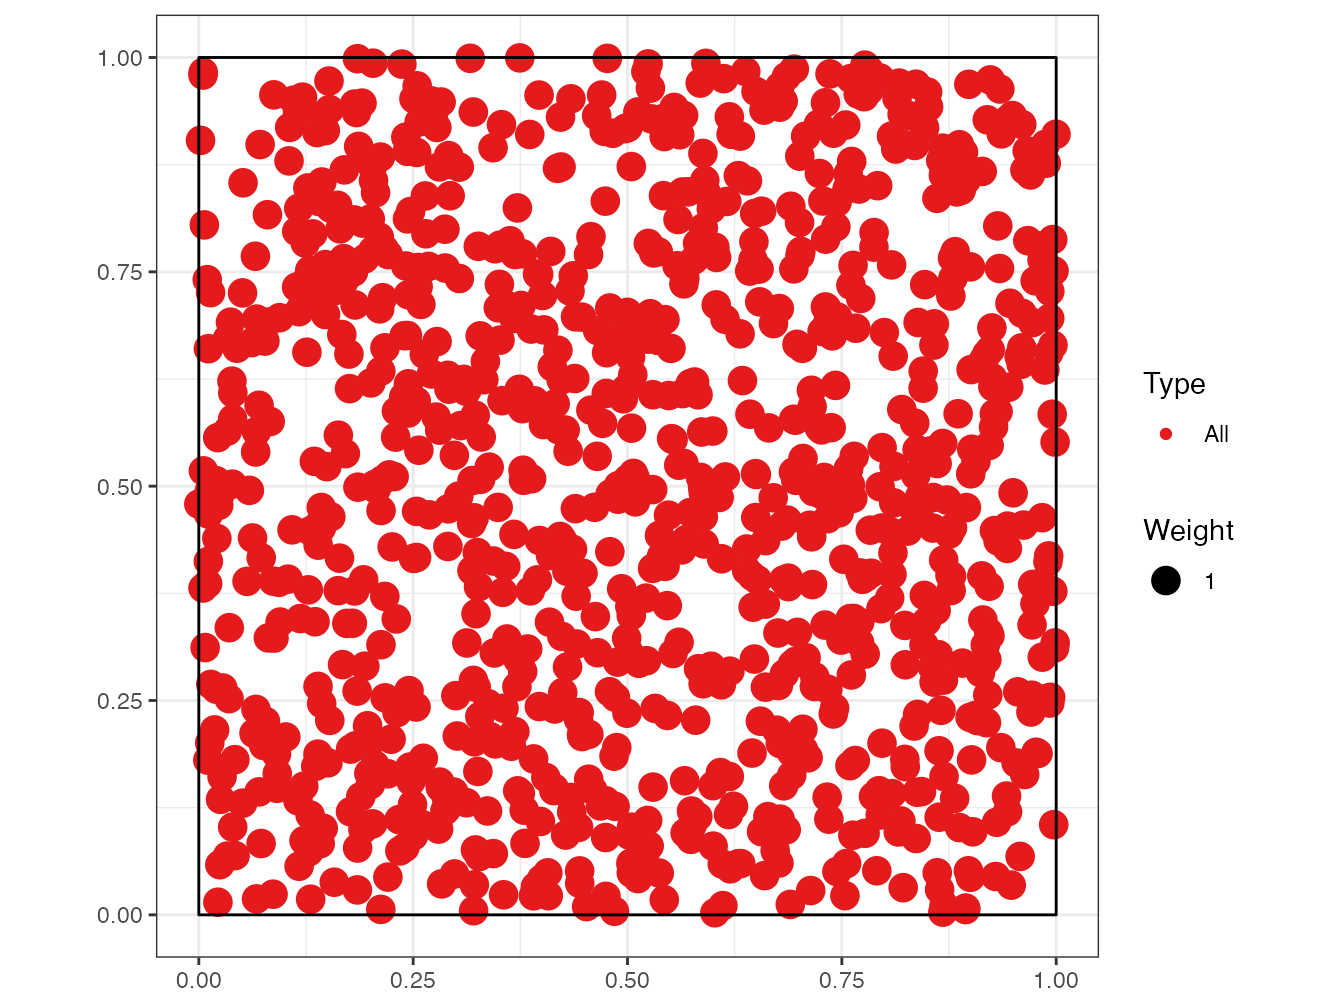
\includegraphics[width=0.8\linewidth]{travailleR_files/figure-latex/tar_read_4-1} \end{center}

\normalsize

\subsection{Contrôle de source}\label{contruxf4le-de-source}

Les fichiers de \textbf{targets} doivent être inclus au contrôle de source.
De cette façon, les calculs effectués localement ne seront pas répétés par GitHub Actions (chapitre \ref{chap-ci}) et la construction du document sera rapide.

\chapter{Package}\label{chap-package}

\toc{1}

Les packages de R permettent d'étendre les fonctionnalités du logiciel par du code fourni par la communauté des développeurs.
Ils sont la clé du succès de R parce qu'ils permettent de diffuser rapidement de nouvelles méthodes issues de la recherche ou d'ajouter de nouveaux outils qui peuvent devenir des standards, comme le \textbf{tidyverse}.

Il est utile de produire un package quand on a écrit des nouvelles fonctions qui forment un ensemble cohérent.
Un package à usage personnel ou limité à une équipe de travail est simple à mettre en place et le temps gagné en utilisant facilement la version à jour de chaque fonction amortit très rapidement le temps consacré à la fabrication du package.
Ce type de package a vocation à être hébergé sur GitHub.

Des packages à usage plus large, qui fournissent par exemple le code correspondant à une méthode publiée, sont placés dans le dépôt CRAN, d'où ils pourront être installés par la commande standard \texttt{install.packages()}.
CRAN effectue des vérifications poussées du code et n'accepte que les packages passant sans aucun avertissement sa batterie de tests.
Ils doivent respecter la politique\footnote{\url{https://cran.r-project.org/web/packages/policies.html}} du dépôt.

La documentation pour la création de packages est abondante.
L'ouvrage de référence est celui de \textcite{Wickham2015}, à consulter en tant que référence.

L'approche utilisée ici consiste à créer un premier package très rapidement pour comprendre que la démarche est assez simple.
Il sera ensuite enrichi des éléments nécessaires à un package diffusé à d'autres utilisateurs que son concepteur: une documentation complète et des tests de bon fonctionnement notamment.

\section{Premier package}\label{premier-package}

Cette introduction reprend les recommandations du blog \emph{Créer un package en quelques minutes}\footnote{\url{https://thinkr.fr/creer-package-r-quelques-minutes/}} de ThinkR.

\subsection{Création}\label{cruxe9ation}

Les packages ont une organisation stricte dans une structure de fichiers et de répertoires figée.
Il est possible de créer cette structure manuellement mais des packages spécialisés peuvent s'en charger:

\begin{itemize}
\tightlist
\item
  \textbf{usethis} automatise la création des dossiers;
\item
  \textbf{roxygen2} permet d'automatiser la documentation obligatoire des packages;
\item
  \textbf{devtools} est la boîte à outils du développeur, permettant notamment de construire et tester les packages;
\end{itemize}

Les trois sont à installer en premier lieu:

\scriptsize

\begin{Shaded}
\begin{Highlighting}[]
\FunctionTok{install.packages}\NormalTok{(}\FunctionTok{c}\NormalTok{(}\StringTok{"usethis"}\NormalTok{, }\StringTok{"roxygen2"}\NormalTok{, }\StringTok{"devtools"}\NormalTok{))}
\end{Highlighting}
\end{Shaded}

\normalsize

Le package à créer sera un projet RStudio.
Dans le menu des projets, sélectionner \enquote{New Project \textgreater{} New Directory \textgreater{} R package using devtools\ldots{}}, choisir le nom du projet et son dossier parent.
Le package s'appellera \textbf{multiple}, dans le dossier \texttt{\%LOCALAPPDATA\%\textbackslash{}ProjetsR} en suivant les recommandations de la section \ref{sec:solution-dossiers}.

Le nom du package doit respecter les contraintes des noms de projets: pas de caractères spéciaux, pas d'espaces\ldots{}
Il doit aussi être évocateur de l'objet du package.
Si le package doit être diffusé, toute sa documentation sera rédigée en Anglais, y compris son nom.

La structure minimale est crée:

\begin{itemize}
\tightlist
\item
  un fichier \texttt{DESCRIPTION} qui indique que le dossier contient un package et précise au minimum son nom;
\item
  un fichier \texttt{NAMESPACE} qui déclare comment le package intervient dans la gestion des noms des objets de R (son contenu sera mis à jour par \textbf{roxygen2});
\item
  un dossier \texttt{R} qui contient le code des fonctions offertes par le package (vide à ce stade).
\end{itemize}

Le package peut être testé tout de suite: dans la fenêtre \emph{Build} de RStudio, cliquer sur \enquote{Install and Restart} construit le package et le charge dans R, après avoir redémarré le programme pour éviter tout conflit.

Dans la fenêtre \emph{Packages}, \textbf{multiple} est maintenant visible.
Il est chargé, mais ne contient rien.

\subsection{Première fonction}\label{premiuxe8re-fonction}

\subsubsection{Fichiers}\label{fichiers}

Les fonctions sont placées dans un ou plusieurs fichier \texttt{.R} dans le dossier \texttt{R}.
L'organisation de ces fichiers est libre.
Pour cet exemple, un fichier du nom de chaque fonction sera créé.
Des fichiers regroupant les fonctions similaires ou un seul fichier contenant tout le code sont des choix possibles.

Le choix fait ici est le suivant:

\begin{itemize}
\tightlist
\item
  un fichier qui contiendra le code commun à tout le package: \texttt{package.R};
\item
  un fichier commun à toutes les fonctions: \texttt{fonctions.R}.
\end{itemize}

\subsubsection{Création}\label{cruxe9ation-1}

La première fonction, \texttt{double()}, est créée et enregistrée dans le fichier \texttt{fonctions.R}:

\scriptsize

\begin{Shaded}
\begin{Highlighting}[]
\NormalTok{double }\OtherTok{\textless{}{-}} \ControlFlowTok{function}\NormalTok{(number) \{}
  \FunctionTok{return}\NormalTok{(}\DecValTok{2} \SpecialCharTok{*}\NormalTok{ number)}
\NormalTok{\}}
\end{Highlighting}
\end{Shaded}

\normalsize

A ce stade, la fonction est interne au package et n'est pas accessible depuis l'environnement de travail.
Pour s'en persuader, construire le package (\emph{Install and Restart}) et vérifier le bon fonctionnement de la fonction:
*

\scriptsize

\begin{Shaded}
\begin{Highlighting}[]
\FunctionTok{double}\NormalTok{(}\DecValTok{2}\NormalTok{)}
\end{Highlighting}
\end{Shaded}

\begin{verbatim}
## [1] 4
\end{verbatim}

\normalsize

Le résultat est un vecteur composé de deux 0 parce que la fonction appelée est un homonyme du package \textbf{base} (voir sa documentation en tapant \texttt{?double}):

\scriptsize

\begin{Shaded}
\begin{Highlighting}[]
\NormalTok{base}\SpecialCharTok{::}\FunctionTok{double}\NormalTok{(}\DecValTok{2}\NormalTok{)}
\end{Highlighting}
\end{Shaded}

\begin{verbatim}
## [1] 0 0
\end{verbatim}

\normalsize

Pour que la fonction de notre package soit visible, elle doit être \emph{exportée} en la déclarant dans le fichier \texttt{NAMESPACE}.
C'est le travail de \textbf{roxygen2} qui gère en même temps la documentation de chaque fonction.
Pour l'activer, placer le curseur dans la fonction et appeler le menu \enquote{Code \textgreater{} Insert Roxygen Skeleton}.
Des commentaires sont ajoutés avant la fonction:

\scriptsize

\begin{Shaded}
\begin{Highlighting}[]
\CommentTok{\#\textquotesingle{} Title}
\CommentTok{\#\textquotesingle{}}
\CommentTok{\#\textquotesingle{} @param number }
\CommentTok{\#\textquotesingle{}}
\CommentTok{\#\textquotesingle{} @return}
\CommentTok{\#\textquotesingle{} @export}
\CommentTok{\#\textquotesingle{}}
\CommentTok{\#\textquotesingle{} @examples}
\NormalTok{double }\OtherTok{\textless{}{-}} \ControlFlowTok{function}\NormalTok{(number) \{}
  \FunctionTok{return}\NormalTok{(}\DecValTok{2} \SpecialCharTok{*}\NormalTok{ number)}
\NormalTok{\}}
\end{Highlighting}
\end{Shaded}

\normalsize

Les commentaires à destination de \textbf{roxygen2} commencent par \texttt{\#\textquotesingle{}}:

\begin{itemize}
\tightlist
\item
  la première ligne contient le titre de la fonction, c'est-à-dire un descriptif très court: son nom en général;
\item
  la ligne suivante (séparée par un saut de ligne) peut contenir sa description (rubrique \emph{Description} dans l'aide);
\item
  la suivante (après un autre saut de ligne) peut contenir plus d'informations (rubrique \emph{Details} dans l'aide);
\item
  les arguments de la fonction sont décrits par les lignes \texttt{@param};
\item
  \texttt{@return} décrit le résultat de la fonction;
\item
  \texttt{@export} déclare que la fonction est exportée: elle sera donc utilisable dans l'environnement de travail;
\item
  des exemples peuvent être ajoutés.
\end{itemize}

La documentation doit être complétée:

\scriptsize

\begin{Shaded}
\begin{Highlighting}[]
\CommentTok{\#\textquotesingle{} double}
\CommentTok{\#\textquotesingle{} }
\CommentTok{\#\textquotesingle{} Double value of numbers.}
\CommentTok{\#\textquotesingle{}}
\CommentTok{\#\textquotesingle{} Calculate the double values of numbers.}
\CommentTok{\#\textquotesingle{} }
\CommentTok{\#\textquotesingle{} @param number a numeric vector.}
\CommentTok{\#\textquotesingle{}}
\CommentTok{\#\textquotesingle{} @return A vector of the same length as \textasciigrave{}number\textasciigrave{} containing the }
\CommentTok{\#\textquotesingle{}   transformed values.}
\CommentTok{\#\textquotesingle{} @export}
\CommentTok{\#\textquotesingle{}}
\CommentTok{\#\textquotesingle{} @examples}
\CommentTok{\#\textquotesingle{} double(2)}
\CommentTok{\#\textquotesingle{} double(1:4)}
\NormalTok{double }\OtherTok{\textless{}{-}} \ControlFlowTok{function}\NormalTok{(number) \{}
  \FunctionTok{return}\NormalTok{(}\DecValTok{2} \SpecialCharTok{*}\NormalTok{ number)}
\NormalTok{\}}
\end{Highlighting}
\end{Shaded}

\normalsize

Ne pas hésiter à s'inspirer de l'aide de fonctions existantes pour respecter les standards de R (ici: \texttt{?log}):

\begin{itemize}
\tightlist
\item
  penser que les fonctions sont normalement vectorielles: \texttt{number} est par défaut un vecteur, pas un scalaire;
\item
  certains éléments commencent par une majuscule et se terminent par un point parce que ce sont des paragraphes dans le fichier d'aide;
\item
  le titre n'a pas de point final;
\item
  la description des paramètres ne commence pas par une majuscule.
\end{itemize}

La prise en compte des changements dans la documentation nécessitent d'appeler la fonction \texttt{roxygenize()}.
Dans la fenêtre \emph{Build}, le menu \enquote{More \textgreater{} Document} permet de le faire.
Ensuite, construire le package (\emph{Install and Restart}) et vérifier le résultat en exécutant la fonction et en affichant son aide:

\scriptsize

\begin{Shaded}
\begin{Highlighting}[]
\NormalTok{?double}
\end{Highlighting}
\end{Shaded}

\normalsize

Il est possible d'automatiser la mise à jour de la documentation à chaque construction du package par le menu \enquote{Build \textgreater{} Configure Build Tools\ldots{}}: cliquer sur \enquote{Configure} et cocher la case \enquote{Automatically reoxygenize when running Install and Restart}.
C'est un choix efficace pour un petit package mais pénalisant quand le temps de mise à jour de la documentation s'allonge avec la complexité du package. La reconstruction du package est le plus souvent utilisée pour tester des modifications du code: sa rapidité est essentielle.

La documentation pour \textbf{roxygen2} supporte le format Markdown\footnote{\url{https://roxygen2.r-lib.org/articles/markdown.html}}.

A ce stade, le package est fonctionnel: il contient une fonction et un début de documentation.
Il est temps de lancer une vérification de son code: dans la fenêtre \emph{Build}, cliquer sur \enquote{Check} ou utiliser la commande \texttt{devtools::check()}.
L'opération \emph{réoxygène} le package (met à jour sa documentation), effectue un grand nombre de tests et renvoie la liste des erreurs, avertissements et notes détectées.
L'objectif est toujours de n'avoir aucune alerte: elles doivent être traitées immédiatement.
Par exemple, le retour suivant est un avertissement sur la non-conformité de la licence déclarée:

\begin{verbatim}
> checking DESCRIPTION meta-information ... WARNING
  Non-standard license specification:
    `use_gpl3_license()`
  Standardizable: FALSE

0 errors v | 1 warning x | 0 notes v
Erreur : R CMD check found WARNINGs
\end{verbatim}

Pour la corriger, mettre à jour, exécuter la commande de mise à jour de la licence, en commençant par votre nom:

\scriptsize

\begin{Shaded}
\begin{Highlighting}[]
\FunctionTok{options}\NormalTok{(}\AttributeTok{usethis.full\_name =} \StringTok{"Eric Marcon"}\NormalTok{)}
\NormalTok{usethis}\SpecialCharTok{::}\FunctionTok{use\_gpl3\_license}\NormalTok{()}
\end{Highlighting}
\end{Shaded}

\normalsize

La liste des licences valides est fournie par R\footnote{\url{https://svn.r-project.org/R/trunk/share/licenses/license.db}}.

Après correction, relancer les tests jusqu'à la disparition des alertes.

\subsection{Contrôle de source}\label{sec:package-cds}

Il est temps de placer le code sous contrôle de source.

Activer le contrôle de source dans les options du projet (figure \ref{fig:git-Project}).
Redémarrer RStudio à la demande.

Créer un dépôt sur GitHub et y pousser le dépôt local, comme expliqué dans le chapitre \ref{chap-git}.

Créer le fichier \texttt{README.md}:

\begin{verbatim}
# multiple

An R package to compute mutiple of numbers.
\end{verbatim}

Le développement du package est ponctué par de nombreux commits à chaque modification et une publication (push) à chaque étape, validée par une incrémentation du numéro de version.

\subsection{package.R}\label{package.r}

Le fichier \texttt{package.R} est destiné à recevoir le code R et surtout les commentaires pour \textbf{roxygen2} qui concernent l'ensemble du package.
Ce fichier peut aussi être nommé \texttt{multiple-package.R}, en préfixant son nom par celui du package, par souci de compatibilité avec \textbf{usethis}.
Il peut d'ailleurs être créé sous ce nom par la commande:

\scriptsize

\begin{Shaded}
\begin{Highlighting}[]
\NormalTok{usethis}\SpecialCharTok{::}\FunctionTok{use\_package\_doc}\NormalTok{()}
\end{Highlighting}
\end{Shaded}

\normalsize

Le premier bloc de commentaire fournira l'aide du package (\texttt{?multiple}).

\begin{verbatim}
#' @keywords internal 
"_PACKAGE"
\end{verbatim}

Le mot-clé ``\_PACKAGE'' indique que la documentation du package doit être produite.
Elle pourrait être écrite dans le bloc, avec une syntaxe identique à celle des fonctions, mais son contenu par défaut est celui du champ \texttt{Description} du fichier \texttt{DESCRIPTION}.
Le mot clé \texttt{internal} masque la documentation du package dans le sommaire de son aide.

La documentation est mise à jour par la commande \texttt{roxygen2::roxygenise()}.
Après reconstruction du package, vérifier que l'aide est est apparue: \texttt{?multiple}.

\section{Organisation du package}\label{organisation-du-package}

\subsection{Fichier DESCRIPTION}\label{sec:package-description}

Le fichier doit être complété:

\begin{verbatim}
Package: multiple
Title: Calculate multiples of numbers
Version: 0.0.0.9000
Authors@R: 
  person(given = "Eric",
           family = "Marcon",
           role = c("aut", "cre"),
           email = "e.marcon@free.fr",
           comment = c(ORCID = "0000-0002-5249-321X"))
Description: Simple computation of multiples of numbers, 
  including fast algorithms for integers.
License: GPL-3
Encoding: UTF-8
LazyData: true
Roxygen: list(markdown = TRUE)
RoxygenNote: 7.1.1
\end{verbatim}

Le nom du package est figé et ne doit pas être modifié.

Son titre doit décrire en une ligne à quoi il sert.
Le titre est affiché dans la fenêtre \emph{Packages} à côté des noms des packages.

La version doit respecter les conventions:

\begin{itemize}
\tightlist
\item
  Le premier nombre est la version majeure, 0 tant que le package n'est pas stable puis 1.
  La version majeure ne change que si le package n'est plus compatible avec ses versions précédentes, ce qui oblige les utilisateurs à modifier leur code.
\item
  Le deuxième est la version mineure, incrémentée quand des fonctionnalités nouvelles sont ajoutées.
\item
  Le troisième est la version de correction: 0 à l'origine, incrémentée à chaque correction de code sans nouvelle fonctionnalité.
\item
  Le quatrième est réservé au développement, et commence à 9000.
  Il est incrémenté à chaque version instable et disparaît quand une nouvelle version stable (\emph{release}) est produite.
\end{itemize}

Exemple: une correction de bug sur la version 1.3.0 produit la version 1.3.1.
Les versions de développement suivantes (instables, non destinées à l'usage en production) sont 1.3.1.9000 puis 1.3.1.9001, etc.
Le numéro de version doit être mis à jour à chaque fois que le package est poussé sur GitHub.
Quand le développement est stabilisé, la nouvelle version, destinée à être utilisée en production, est 1.3.2 si elle n'apporte pas de nouvelle fonctionnalité ou 1.4.0 dans le cas contraire.

La description des auteurs est assez lourde mais simple à comprendre.
Les identifiants Orcid des auteurs académiques peuvent être utilisés.
Si le package a plusieurs auteurs, ils sont placés dans une fonction \texttt{c()}: \texttt{c(person(...),\ person(...))} pour deux auteurs.
Dans ce cas, il faut préciser le rôle de chacun:

\begin{itemize}
\tightlist
\item
  \enquote{cre} pour le créateur du package;
\item
  \enquote{aut} pour un auteur parmi les autres;
\item
  \enquote{ctb} pour un contributeur, qui peut avoir signalé un bug ou fourni un peu de code.
\end{itemize}

La description du package en un paragraphe permet de donner plus d'informations.

La licence précise la façon dont le package peut être utilisé et modifié.
GPL-3 est une bonne valeur par défaut, mais d'autres choix sont possibles\footnote{\url{https://r-pkgs.org/description.html\#description-license}}.

L'option \texttt{LazyData} signifie que les données d'exemples fournies avec le package peuvent être utilisées sans les appeler au préalable par la fonction \texttt{data()}: c'est le standard actuel.

Enfin, les deux dernières lignes sont gérées par \textbf{roxygen2}.

\subsection{Fichier NEWS.md}\label{fichier-news.md}

Le fichier \texttt{NEWS.md} contient l'historique du package.
Les nouvelles versions sont ajoutées en haut du fichier.

Créer une première version du fichier:

\begin{verbatim}
# multiple 0.0.0.9000

## New features

* Initial version of the package
\end{verbatim}

Les titres de premier niveau doivent contenir le nom du package et sa version.
Les titres de niveau 2 sont libres, mais contiennent en général des rubriques comme \enquote{New features} et \enquote{Bug Fixes}.

Pour ne pas multiplier les versions décrites, il est conseillé de modifier la version en cours et de compléter la documentation jusqu'au changement de version de correction (troisième nombre).
Ensuite, l'entrée correspondant à cette version reste figée et une nouvelle entrée est ajoutée.

\section{Vignette}\label{vignette}

Une vignette est indispensable pour documenter correctement le package:

\scriptsize

\begin{Shaded}
\begin{Highlighting}[]
\NormalTok{usethis}\SpecialCharTok{::}\FunctionTok{use\_vignette}\NormalTok{(}\StringTok{"multiple"}\NormalTok{)}
\end{Highlighting}
\end{Shaded}

\normalsize

Le fichier \texttt{multiple.Rmd} est créé dans le dossier \texttt{vignettes}.
Ajouter un sous-titre dans son entête: la description courte du package:

\begin{verbatim}
title: "multiple"
subtitle: "Multiples of numbers"
\end{verbatim}

Le reste de l'entête permet à R de construire la vignette à partir de code R Markdown.

Le corps de la vignette contient par défaut du code R pour déclarer les options de présentation des bouts de code et le chargement du package.
Une introduction à l'utilisation du package doit être écrite dans ce document, en R Markdown.

Pendant le développement du package, la vignette peut être construite manuellement en exécutant:

\scriptsize

\begin{Shaded}
\begin{Highlighting}[]
\NormalTok{devtools}\SpecialCharTok{::}\FunctionTok{build\_vignettes}\NormalTok{(}\StringTok{"multiple"}\NormalTok{) }
\end{Highlighting}
\end{Shaded}

\normalsize

Les fichiers produits sont placés dans \texttt{doc/}: ouvrir le fichier \texttt{.html} pour contrôler le résultat.

RStudio ne crée pas la vignette du package quand la commande \enquote{Install and Restart} de la fenêtre Build est appelée.
Pour une installation complète, deux solutions sont possibles:

\begin{itemize}
\tightlist
\item
  Construire le fichier source du package (\enquote{Build \textgreater{} More \textgreater{} Build Source Package}) puis l'installer (\enquote{Packages \textgreater{} Install \textgreater{} Install from \textgreater{} Package Archive file}).
  Le fichier source se trouve à côté de celui du projet.
\item
  Pousser le code du package sur GitHub puis exécuter:
\end{itemize}

\scriptsize

\begin{Shaded}
\begin{Highlighting}[]
\NormalTok{remotes}\SpecialCharTok{::}\FunctionTok{install\_github}\NormalTok{(}\StringTok{"multiple"}\NormalTok{, }\AttributeTok{build\_vignettes =} \ConstantTok{TRUE}\NormalTok{)}
\end{Highlighting}
\end{Shaded}

\normalsize

La vignette peut ensuite être affichée par la commande:

\scriptsize

\begin{Shaded}
\begin{Highlighting}[]
\FunctionTok{vignette}\NormalTok{(}\StringTok{"multiple"}\NormalTok{)}
\end{Highlighting}
\end{Shaded}

\normalsize

\section{pkgdown}\label{pkgdown}

Le package \textbf{pkgdown} permet de créer un site d'accompagnement du package\footnote{Exemple: \url{https://EricMarcon.github.io/entropart/}}, qui reprend le fichier \texttt{README.md} comme page d'accueil, la vignette dans une rubrique \enquote{Get Started}, l'ensemble des fichiers d'aide avec leurs exemples exécutés (section \enquote{Reference}), le fichier \texttt{NEWS.md} pour un historique du package (section \enquote{Changelog}) et des informations du fichier \texttt{DESCRIPTION}.

Créer le site avec \textbf{usethis}:

\scriptsize

\begin{Shaded}
\begin{Highlighting}[]
\NormalTok{usethis}\SpecialCharTok{::}\FunctionTok{use\_pkgdown}\NormalTok{()}
\end{Highlighting}
\end{Shaded}

\normalsize

Construire ensuite le site.
Cette commande sera exécutée à nouveau à chaque changement de version du package:

\scriptsize

\begin{Shaded}
\begin{Highlighting}[]
\NormalTok{pkgdown}\SpecialCharTok{::}\FunctionTok{build\_site}\NormalTok{()}
\end{Highlighting}
\end{Shaded}

\normalsize

Le site est placé dans le dossier \texttt{docs}.
Ouvrir le fichier \texttt{index.htm} avec un navigateur web pour le visualiser.
Dès que le projet sera poussé sur GitHub, activer les pages du dépôt pour que le site soit visible en ligne (voir section \ref{sec:github-pages}).

\textbf{pkgdown} place le site dans le dossier \texttt{docs}.

Ajouter l'adresse des pages GitHub dans une nouvelle ligne du fichier \texttt{DESCRIPTION}:

\begin{verbatim}
URL: https://GitHubID.github.io/multiple
\end{verbatim}

L'ajouter aussi dans le fichier \texttt{\_pkgdown.yml} qui a été créé vide, ainsi que l'option suivante:

\begin{verbatim}
url: https://GitHubID.github.io/multiple

development:
  mode: auto
\end{verbatim}

\textbf{pkgdown} place le site dans le dossier \texttt{docs/dev} si le site d'une version stable (à trois nombres) du package existe dans \texttt{docs} et que la version en cours est une version de développement (à quatre nombres).
De cette façon, les utilisateurs d'une version de production du package ont accès au site sans qu'il soit perturbé par les versions de développement.

Le site peut être enrichi de plusieurs façons:

\begin{itemize}
\tightlist
\item
  En ajoutant des articles au format R Markdown dans le dossier \texttt{vignettes/articles}.
  La vignette ne peut pas mobiliser d'importantes ressources de calcul pour présenter des exemples parce qu'elle est construite en même temps que le package.
  Les articles sont générés par \textbf{pkgdown}, indépendamment, et peuvent donc être plus ambitieux;
\item
  En améliorant sa présentation (regroupement des fonctions par thèmes, ajout de badges, d'un sticker\footnote{L'application Shiny \textbf{hexmake} permet de créer facilement un sticker: \url{https://connect.thinkr.fr/hexmake/}}\ldots): se référer à la vignette de \textbf{pkgdown}.
\end{itemize}

Pour enrichir la documentation du package, il est possible d'utiliser un fichier \texttt{README.Rmd} au format R Markdown, à tricoter pour créer le \texttt{README.md} standard de GitHub, utilisé comme page d'accueil du site \textbf{pkgdown}, qui peut de cette façon présenter des exemples d'utilisation du code.
La démarche est détaillée dans \emph{R Packages}\footnote{\url{https://r-pkgs.org/release.html?q=readme\#readme-rmd}}.
La complexité ajoutée est à comparer au gain obtenu: une page d'accueil simple (sans code) avec des liens vers la vignette et les articles est plus simple à mettre en œuvre.

\section{Code spécifique aux packages}\label{code-spuxe9cifique-aux-packages}

\subsection{Importation de fonctions}\label{importation-de-fonctions}

Créons une nouvelle fonction dans \texttt{fonctions.R} qui ajoute un bruit aléatoire à la valeur double:

\scriptsize

\begin{Shaded}
\begin{Highlighting}[]
\NormalTok{fuzzydouble }\OtherTok{\textless{}{-}} \ControlFlowTok{function}\NormalTok{(number, }\AttributeTok{sd =} \DecValTok{1}\NormalTok{) \{}
  \FunctionTok{return}\NormalTok{(}\DecValTok{2} \SpecialCharTok{*}\NormalTok{ number }\SpecialCharTok{+} \FunctionTok{rnorm}\NormalTok{(}\FunctionTok{length}\NormalTok{(number), }\DecValTok{0}\NormalTok{, sd))}
\NormalTok{\}}
\end{Highlighting}
\end{Shaded}

\normalsize

Le bruit est tiré dans une loi normale centrée d'écart-type \texttt{sd} et ajouté à la valeur calculée.

\texttt{rnorm()} est une fonction du package \textbf{stats}.
Même si le package est systématiquement chargé par R, le package d'appartenance de la fonction doit obligatoirement être déclaré: les seules exceptions sont les fonctions du package \textbf{base}.

Le package \textbf{stats} doit d'abord être déclaré dans \texttt{DESCRIPTION} qui contient une instruction \texttt{Imports:}.
Tous les packages utilisés par le code de \textbf{multiple} seront listés, séparés par des virgules.

\begin{verbatim}
Imports: stats
\end{verbatim}

Cette \enquote{importation} signifie simplement que le package \textbf{stats} doit être chargé, mais pas nécessairement attaché (voir section \ref{sec:environnements}), pour que \textbf{multiple} fonctionne.

Ensuite, la fonction \texttt{rnorm()} doit être trouvable dans l'environnement du package \textbf{multiple}.
Il y a plusieurs façons de remplir cette obligation.
D'abord, le commentaire suivant pourrait être fourni pour \textbf{roxygen2}:

\scriptsize

\begin{Shaded}
\begin{Highlighting}[]
\CommentTok{\#\textquotesingle{} @import stats}
\end{Highlighting}
\end{Shaded}

\normalsize

Tout l'espace de nom du package \textbf{stats} serait attaché et accessible au package \textbf{multiple}.
Ce n'est pas une bonne pratique parce qu'elle multiplie les risques de conflits de noms (voir section \ref{sec:environnements}).
Notons que la notion d'importation utilisée ici est différente de celle de \texttt{DESCRIPTION}, bien qu'elles aient le même nom.

Il est préférable d'importer uniquement la fonction \texttt{rnorm()} en la déclarant dans la documentation de la fonction:

\scriptsize

\begin{Shaded}
\begin{Highlighting}[]
\CommentTok{\#\textquotesingle{} @importFrom stats rnorm}
\end{Highlighting}
\end{Shaded}

\normalsize

Ce n'est pas une pratique idéale non plus parce que l'origine de la fonction n'apparaîtrait pas clairement dans le code du package.

La bonne pratique est de ne rien importer (au sens de \textbf{roxygen2}) et de qualifier systématiquement les fonctions d'autres packages avec la syntaxe \texttt{package::fonction()}.
C'est la solution retenue ici parce que la directive \texttt{@importFrom} importerait la fonction dans tout le package \textbf{multiple}, pas seulement dans la fonction \texttt{fuzzydouble()}, au risque de créer des effets de bord (modifier le comportement d'une autre fonction du package qui n'assumerait pas l'importation de \texttt{rnorm()}).
Finalement, le code de la fonction est le suivant:

\scriptsize

\begin{Shaded}
\begin{Highlighting}[]
\CommentTok{\#\textquotesingle{} fuzzydouble}
\CommentTok{\#\textquotesingle{} }
\CommentTok{\#\textquotesingle{} Double value of numbers with an error}
\CommentTok{\#\textquotesingle{} }
\CommentTok{\#\textquotesingle{} Calculate the double values of numbers }
\CommentTok{\#\textquotesingle{} and add a random error to the result.}
\CommentTok{\#\textquotesingle{}}
\CommentTok{\#\textquotesingle{} @param number a numeric vector.}
\CommentTok{\#\textquotesingle{} @param sd the standard deviation of the Gaussian error added.}
\CommentTok{\#\textquotesingle{}}
\CommentTok{\#\textquotesingle{} @return A vector of the same length as \textasciigrave{}number\textasciigrave{}}
\CommentTok{\#\textquotesingle{}  containing the transformed values.}
\CommentTok{\#\textquotesingle{} @export}
\CommentTok{\#\textquotesingle{}}
\CommentTok{\#\textquotesingle{} @examples}
\CommentTok{\#\textquotesingle{} fuzzydouble(2)}
\CommentTok{\#\textquotesingle{} fuzzydouble(1:4)}

\NormalTok{fuzzydouble }\OtherTok{\textless{}{-}} \ControlFlowTok{function}\NormalTok{(number, }\AttributeTok{sd =} \DecValTok{1}\NormalTok{) \{}
  \FunctionTok{return}\NormalTok{(}\DecValTok{2} \SpecialCharTok{*}\NormalTok{ number }\SpecialCharTok{+}\NormalTok{ stats}\SpecialCharTok{::}\FunctionTok{rnorm}\NormalTok{(}\FunctionTok{length}\NormalTok{(number), }\DecValTok{0}\NormalTok{, sd))}
\NormalTok{\}}
\end{Highlighting}
\end{Shaded}

\normalsize

\subsection{Méthodes S3}\label{muxe9thodes-s3}

Les méthodes S3 sont présentées en section \ref{sec:S3}.

\subsubsection{Classes}\label{classes}

Les objets appartiennent à des classes:

\scriptsize

\begin{Shaded}
\begin{Highlighting}[]
\CommentTok{\# Classe d\textquotesingle{}un nombre}
\FunctionTok{class}\NormalTok{(}\DecValTok{2}\NormalTok{)}
\end{Highlighting}
\end{Shaded}

\begin{verbatim}
## [1] "numeric"
\end{verbatim}

\begin{Shaded}
\begin{Highlighting}[]
\CommentTok{\# Classe d\textquotesingle{}une fonction}
\FunctionTok{class}\NormalTok{(sum)}
\end{Highlighting}
\end{Shaded}

\begin{verbatim}
## [1] "function"
\end{verbatim}

\normalsize

En plus des classes de base, les développeurs peuvent en créer d'autres.

\subsubsection{Méthodes}\label{muxe9thodes}

L'intérêt de créer de nouvelles classes est de leur adapter des méthodes existantes, le cas le plus courant étant \texttt{plot()}.
Il s'agit d'une méthode générique, c'est-à-dire un modèle de fonction, sans code, à décliner selon la classe d'objet à traiter.

\scriptsize

\begin{Shaded}
\begin{Highlighting}[]
\NormalTok{plot}
\end{Highlighting}
\end{Shaded}

\begin{verbatim}
## function (x, y, ...) 
## UseMethod("plot")
## <bytecode: 0x133742b10>
## <environment: namespace:base>
\end{verbatim}

\normalsize

Il existe dans R de nombreuses déclinaisons de \texttt{plot} qui sont des fonctions dont le nom est de la forme \texttt{plot.class()}.
\textbf{stats} fournit une fonction \texttt{plot.lm()} pour créer une figure à partir d'un modèle linéaire.
De nombreux packages créent des classes adaptées à leurs objets et proposent une méthode \texttt{plot} pour chaque classe.
Les fonctions peuvent être listées:

\scriptsize

\begin{Shaded}
\begin{Highlighting}[]
\CommentTok{\# Quelques fonctions plot()}
\FunctionTok{head}\NormalTok{(}\FunctionTok{methods}\NormalTok{(plot))}
\end{Highlighting}
\end{Shaded}

\begin{verbatim}
## [1] "plot,ANY-method"      "plot,color-method"   
## [3] "plot.AccumCurve"      "plot.acf"            
## [5] "plot.ACF"             "plot.adaptivedensity"
\end{verbatim}

\begin{Shaded}
\begin{Highlighting}[]
\CommentTok{\# Nombre total}
\FunctionTok{length}\NormalTok{(}\FunctionTok{methods}\NormalTok{(plot))}
\end{Highlighting}
\end{Shaded}

\begin{verbatim}
## [1] 156
\end{verbatim}

\normalsize

Inversement, les méthodes disponibles pour une classe peuvent être affichées:

\scriptsize

\begin{Shaded}
\begin{Highlighting}[]
\FunctionTok{methods}\NormalTok{(}\AttributeTok{class =} \StringTok{"lm"}\NormalTok{)}
\end{Highlighting}
\end{Shaded}

\begin{verbatim}
##  [1] add1           alias          anova         
##  [4] as_flextable   case.names     coerce        
##  [7] confint        cooks.distance deviance      
## [10] dfbeta         dfbetas        drop1         
## [13] dummy.coef     effects        extractAIC    
## [16] family         formula        fortify       
## [19] hatvalues      influence      initialize    
## [22] kappa          labels         logLik        
## [25] model.frame    model.matrix   nobs          
## [28] plot           predict        print         
## [31] proj           qqnorm         qr            
## [34] residuals      response       rstandard     
## [37] rstudent       show           simulate      
## [40] slotsFromS3    summary        variable.names
## [43] vcov          
## see '?methods' for accessing help and source code
\end{verbatim}

\normalsize

La méthode \texttt{print} est utilisée pour afficher tout objet (elle est implicite quand on saisit seulement le nom d'un objet):

\scriptsize

\begin{Shaded}
\begin{Highlighting}[]
\NormalTok{my\_lm }\OtherTok{\textless{}{-}} \FunctionTok{lm}\NormalTok{(dist }\SpecialCharTok{\textasciitilde{}}\NormalTok{ speed, }\AttributeTok{data =}\NormalTok{ cars)}
\CommentTok{\# Equivalent de "\textgreater{} my\_lm"}
\FunctionTok{print}\NormalTok{(my\_lm)}
\end{Highlighting}
\end{Shaded}

\begin{verbatim}
## 
## Call:
## lm(formula = dist ~ speed, data = cars)
## 
## Coefficients:
## (Intercept)        speed  
##     -17.579        3.932
\end{verbatim}

\normalsize

La méthode \texttt{summary} affiche un résumé lisible de l'objet:

\scriptsize

\begin{Shaded}
\begin{Highlighting}[]
\FunctionTok{summary}\NormalTok{(my\_lm)}
\end{Highlighting}
\end{Shaded}

\begin{verbatim}
## 
## Call:
## lm(formula = dist ~ speed, data = cars)
## 
## Residuals:
##     Min      1Q  Median      3Q     Max 
## -29.069  -9.525  -2.272   9.215  43.201 
## 
## Coefficients:
##             Estimate Std. Error t value Pr(>|t|)    
## (Intercept) -17.5791     6.7584  -2.601   0.0123 *  
## speed         3.9324     0.4155   9.464 1.49e-12 ***
## ---
## Signif. codes:  
## 0 '***' 0.001 '**' 0.01 '*' 0.05 '.' 0.1 ' ' 1
## 
## Residual standard error: 15.38 on 48 degrees of freedom
## Multiple R-squared:  0.6511, Adjusted R-squared:  0.6438 
## F-statistic: 89.57 on 1 and 48 DF,  p-value: 1.49e-12
\end{verbatim}

\normalsize

Les autres méthodes ont été créées spécifiquement pour les besoins du package \textbf{stats}.

\subsubsection{Attribution d'un objet à une classe}\label{attribution-dun-objet-uxe0-une-classe}

Pour qu'un objet appartient à une classe, il suffit de le déclarer:

\scriptsize

\begin{Shaded}
\begin{Highlighting}[]
\NormalTok{x }\OtherTok{\textless{}{-}} \DecValTok{1}
\FunctionTok{class}\NormalTok{(x) }\OtherTok{\textless{}{-}} \StringTok{"MyClass"}
\FunctionTok{class}\NormalTok{(x)}
\end{Highlighting}
\end{Shaded}

\begin{verbatim}
## [1] "MyClass"
\end{verbatim}

\normalsize

Une façon plus élégante de le faire est d'ajouter la nouvelle classe à l'ensemble des classes auquel l'objet appartient déjà:

\scriptsize

\begin{Shaded}
\begin{Highlighting}[]
\NormalTok{y }\OtherTok{\textless{}{-}} \DecValTok{1}
\FunctionTok{class}\NormalTok{(y) }\OtherTok{\textless{}{-}} \FunctionTok{c}\NormalTok{(}\StringTok{"MyClass"}\NormalTok{, }\FunctionTok{class}\NormalTok{(y))}
\FunctionTok{class}\NormalTok{(y)}
\end{Highlighting}
\end{Shaded}

\begin{verbatim}
## [1] "MyClass" "numeric"
\end{verbatim}

\normalsize

Il n'y a aucune vérification de cohérence entre la structure réelle de l'objet et une structure de la classe qui serait déclarée ailleurs: le développeur doit s'assurer que les méthodes trouveront bien les bonnes données dans les objets qui déclarent lui appartenir.
Dans le cas contraire, des erreurs se produisent:

\scriptsize

\begin{Shaded}
\begin{Highlighting}[]
\FunctionTok{class}\NormalTok{(y) }\OtherTok{\textless{}{-}} \StringTok{"lm"}
\FunctionTok{tryCatch}\NormalTok{(}\FunctionTok{print}\NormalTok{(y), }\AttributeTok{error =} \ControlFlowTok{function}\NormalTok{(e) }\FunctionTok{print}\NormalTok{(e))}
\end{Highlighting}
\end{Shaded}

\begin{verbatim}
## <simpleError in x$call: $ operator is invalid for atomic vectors>
\end{verbatim}

\normalsize

\subsection{En pratique}\label{en-pratique}

\subsubsection{Création d'une méthode générique}\label{cruxe9ation-dune-muxe9thode-guxe9nuxe9rique}

De nouvelles méthodes génériques peuvent être créées et déclinées selon les classes.

A titre d'exemple, créons une méthode générique \texttt{triple} qui calculera le triple des valeurs dans le package \textbf{multiple}, déclinée en deux fonctions distinctes: une pour les entiers et une pour les réels.
Les calculs sur les nombres entiers plus rapides que ceux sur les réels, ce qui justifie l'effort d'écrire deux versions du code.

\scriptsize

\begin{Shaded}
\begin{Highlighting}[]
\CommentTok{\# Méthode générique}
\NormalTok{triple }\OtherTok{\textless{}{-}} \ControlFlowTok{function}\NormalTok{ (x, ...) \{}
  \FunctionTok{UseMethod}\NormalTok{(}\StringTok{"triple"}\NormalTok{)}
\NormalTok{\}}
\end{Highlighting}
\end{Shaded}

\normalsize

La méthode générique ne contient pas de code au-delà de sa déclaration.
Sa signature (c'est-à-dire l'ensemble de ses arguments) est importante parce que les fonctions dérivées de cette méthode devront obligatoirement avoir les mêmes arguments dans le même ordre et pourront seulement ajouter des arguments supplémentaires avant \texttt{...} (qui est obligatoire).
Comme la nature du premier argument dépendra de la classe de chaque objet, l'usage est de l'appeler \texttt{x}.

La méthode est déclinée en deux fonctions:

\scriptsize

\begin{Shaded}
\begin{Highlighting}[]
\NormalTok{triple.integer}\OtherTok{\textless{}{-}} \ControlFlowTok{function}\NormalTok{ (x, ...)\{}
  \FunctionTok{return}\NormalTok{(x }\SpecialCharTok{*} \DecValTok{3}\DataTypeTok{L}\NormalTok{)}
\NormalTok{\}}
\NormalTok{triple.numeric}\OtherTok{\textless{}{-}} \ControlFlowTok{function}\NormalTok{ (x, ...)\{}
  \FunctionTok{return}\NormalTok{(x }\SpecialCharTok{*} \FloatTok{3.0}\NormalTok{)}
\NormalTok{\}}
\end{Highlighting}
\end{Shaded}

\normalsize

Dans sa version entière, \texttt{x} est multiplié par \texttt{3L}, le suffixe \texttt{L} signifiant que 3 doit être compris comme un entier.
Dans sa version réelle, 3 peut être noté \texttt{3.0} pour montrer clairement qu'il s'agit d'un réel.
Sous R, \texttt{3} sans autre précision est compris comme un réel.

Le choix de la fonction dépend de la classe de l'objet passé en argument.

\scriptsize

\begin{Shaded}
\begin{Highlighting}[]
\CommentTok{\# Argument entier}
\FunctionTok{class}\NormalTok{(}\DecValTok{2}\DataTypeTok{L}\NormalTok{)}
\end{Highlighting}
\end{Shaded}

\begin{verbatim}
## [1] "integer"
\end{verbatim}

\begin{Shaded}
\begin{Highlighting}[]
\CommentTok{\# Résultat entier par la fonction triple.integer}
\FunctionTok{class}\NormalTok{(}\FunctionTok{triple}\NormalTok{(}\DecValTok{2}\DataTypeTok{L}\NormalTok{))}
\end{Highlighting}
\end{Shaded}

\begin{verbatim}
## [1] "integer"
\end{verbatim}

\begin{Shaded}
\begin{Highlighting}[]
\CommentTok{\# Argument réel}
\FunctionTok{class}\NormalTok{(}\DecValTok{2}\NormalTok{)}
\end{Highlighting}
\end{Shaded}

\begin{verbatim}
## [1] "numeric"
\end{verbatim}

\begin{Shaded}
\begin{Highlighting}[]
\CommentTok{\# Résultat réel par la fonction triple.numeric}
\FunctionTok{class}\NormalTok{(}\FunctionTok{triple}\NormalTok{(}\DecValTok{2}\NormalTok{))}
\end{Highlighting}
\end{Shaded}

\begin{verbatim}
## [1] "numeric"
\end{verbatim}

\begin{Shaded}
\begin{Highlighting}[]
\CommentTok{\# Performance}
\FunctionTok{library}\NormalTok{(}\StringTok{"microbenchmark"}\NormalTok{)}
\FunctionTok{microbenchmark}\NormalTok{(}\FunctionTok{triple.integer}\NormalTok{(}\DecValTok{2}\DataTypeTok{L}\NormalTok{), }\FunctionTok{triple.numeric}\NormalTok{(}\DecValTok{2}\NormalTok{), }\FunctionTok{triple}\NormalTok{(}\DecValTok{2}\DataTypeTok{L}\NormalTok{))}
\end{Highlighting}
\end{Shaded}

\begin{verbatim}
## Unit: nanoseconds
##                expr min  lq    mean median    uq    max
##  triple.integer(2L)  82 123  138.58    123 143.5    410
##   triple.numeric(2)  82 123 8399.26    123 123.0 826437
##          triple(2L) 492 492 6942.94    533 533.0 641486
##  neval
##    100
##    100
##    100
\end{verbatim}

\normalsize

La mesure des performances par le package \textbf{microbenchmark} ne montre pas de différence entre les fonctions \texttt{triple.integer()} et \texttt{triple.numeric} comme attendu parce que le temps consacré au calcul lui-même est négligeable en comparaison du temps d'appel de la fonction.
La méthode générique consomme beaucoup plus de temps que les calculs très simples ici.
R teste en effet l'existence de fonctions correspondant à la classe de l'objet passé en argument aux méthodes génériques.
Comme un objet peut appartenir à plusieurs classes, il recherche une fonction adaptée à la première classe, puis aux classes suivantes successivement.
Cette recherche prend beaucoup de temps et justifie de réserver l'usage de méthodes génériques à la lisibilité du code plutôt qu'à une recherche de performance: l'intérêt des méthodes génériques est de fournir à l'utilisateur du code une seule fonction pour un objectif donné (\texttt{plot} pour réaliser une figure) quelles que soient les données à traiter.

\subsubsection{Création d'une classe}\label{cruxe9ation-dune-classe}

Dans un package, on créera des classes si les résultats des fonctions le justifient: structure de liste et identification de la classe à un objet (\enquote{lm} est la classe des modèles linéaires).
Pour toute classe créée, les méthodes \texttt{print}, \texttt{summary} et \texttt{plot} (si une représentation graphique est possible) doivent être écrites.

Ecrivons une fonction \texttt{multiple()} dont le résultat sera un objet d'une nouvelle classe, \enquote{multiple}, qui sera une liste mémorisant les valeurs à multiplier, le multiplicateur et le résultat.

\scriptsize

\begin{Shaded}
\begin{Highlighting}[]
\NormalTok{multiple }\OtherTok{\textless{}{-}} \ControlFlowTok{function}\NormalTok{(number, }\AttributeTok{times =} \DecValTok{1}\NormalTok{) \{}
  \CommentTok{\# Calculate the multiples}
\NormalTok{  y }\OtherTok{\textless{}{-}}\NormalTok{ number }\SpecialCharTok{*}\NormalTok{ times}
  \CommentTok{\# Save in a list}
\NormalTok{  result }\OtherTok{\textless{}{-}} \FunctionTok{list}\NormalTok{(}\AttributeTok{x =}\NormalTok{ number, }\AttributeTok{y =}\NormalTok{ y, }\AttributeTok{times =}\NormalTok{ times)}
  \CommentTok{\# Set the class}
  \FunctionTok{class}\NormalTok{(result) }\OtherTok{\textless{}{-}} \FunctionTok{c}\NormalTok{(}\StringTok{"multiple"}\NormalTok{, }\FunctionTok{class}\NormalTok{(result))}
  \FunctionTok{return}\NormalTok{(result)}
\NormalTok{\}}
\CommentTok{\# Classe du résultat}
\NormalTok{my\_multiple }\OtherTok{\textless{}{-}} \FunctionTok{multiple}\NormalTok{(}\DecValTok{1}\SpecialCharTok{:}\DecValTok{3}\NormalTok{, }\DecValTok{2}\NormalTok{)}
\FunctionTok{class}\NormalTok{(my\_multiple)}
\end{Highlighting}
\end{Shaded}

\begin{verbatim}
## [1] "multiple" "list"
\end{verbatim}

\normalsize

L'appel à la fonction \texttt{multiple()} renvoie un objet de classe \enquote{multiple}, qui est aussi de classe \enquote{list}.
En absence de fonction \texttt{print.multiple()}, R cherche la fonction \texttt{print.list()} qui n'existe pas et se rabat sur la fonction \texttt{print.default()}:

\scriptsize

\begin{Shaded}
\begin{Highlighting}[]
\NormalTok{my\_multiple}
\end{Highlighting}
\end{Shaded}

\begin{verbatim}
## $x
## [1] 1 2 3
## 
## $y
## [1] 2 4 6
## 
## $times
## [1] 2
## 
## attr(,"class")
## [1] "multiple" "list"
\end{verbatim}

\normalsize

La fonction \texttt{print.multiple} doit donc être écrite pour un affichage lisible, limité au résultat:

\scriptsize

\begin{Shaded}
\begin{Highlighting}[]
\NormalTok{print.multiple }\OtherTok{\textless{}{-}} \ControlFlowTok{function}\NormalTok{(x, ...) \{}
  \FunctionTok{print.default}\NormalTok{(x}\SpecialCharTok{$}\NormalTok{y)}
\NormalTok{\}}

\CommentTok{\# Nouvel affichage}
\NormalTok{my\_multiple}
\end{Highlighting}
\end{Shaded}

\begin{verbatim}
## [1] 2 4 6
\end{verbatim}

\normalsize

Les détails peuvent être présentés dans la fonction \texttt{summary}:

\scriptsize

\begin{Shaded}
\begin{Highlighting}[]
\NormalTok{summary.multiple }\OtherTok{\textless{}{-}} \ControlFlowTok{function}\NormalTok{(object, ...) \{}
  \FunctionTok{print.default}\NormalTok{(object}\SpecialCharTok{$}\NormalTok{x)}
  \FunctionTok{cat}\NormalTok{(}\StringTok{"multiplied by"}\NormalTok{, object}\SpecialCharTok{$}\NormalTok{times, }\StringTok{"is:}\SpecialCharTok{\textbackslash{}n}\StringTok{"}\NormalTok{)}
  \FunctionTok{print.default}\NormalTok{(object}\SpecialCharTok{$}\NormalTok{y)}
\NormalTok{\}}

\CommentTok{\# Nouvel affichage}
\FunctionTok{summary}\NormalTok{(my\_multiple)}
\end{Highlighting}
\end{Shaded}

\begin{verbatim}
## [1] 1 2 3
## multiplied by 2 is:
## [1] 2 4 6
\end{verbatim}

\normalsize

Enfin, une fonction \texttt{plot} et une fonction \texttt{autoplot} complètent l'ensemble:

\scriptsize

\begin{Shaded}
\begin{Highlighting}[]
\NormalTok{plot.multiple }\OtherTok{\textless{}{-}} \ControlFlowTok{function}\NormalTok{(x, y, ...) \{}
  \FunctionTok{plot.default}\NormalTok{(}
    \AttributeTok{x =}\NormalTok{ x}\SpecialCharTok{$}\NormalTok{x, }
    \AttributeTok{y =}\NormalTok{ x}\SpecialCharTok{$}\NormalTok{y, }
    \AttributeTok{type =} \StringTok{"p"}\NormalTok{, }
    \AttributeTok{main =} \FunctionTok{paste}\NormalTok{(}\StringTok{"Multiplication by"}\NormalTok{, x}\SpecialCharTok{$}\NormalTok{times), }
\NormalTok{    ...}
\NormalTok{  )}
\NormalTok{\}}

\NormalTok{autoplot.multiple }\OtherTok{\textless{}{-}} \ControlFlowTok{function}\NormalTok{(object, ...) \{}
  \FunctionTok{data.frame}\NormalTok{(}\AttributeTok{x =}\NormalTok{ object}\SpecialCharTok{$}\NormalTok{x, }\AttributeTok{y =}\NormalTok{ object}\SpecialCharTok{$}\NormalTok{y) }\SpecialCharTok{\%\textgreater{}\%} 
\NormalTok{    ggplot2}\SpecialCharTok{::}\FunctionTok{ggplot}\NormalTok{() }\SpecialCharTok{+}
\NormalTok{    ggplot2}\SpecialCharTok{::}\FunctionTok{geom\_point}\NormalTok{(ggplot2}\SpecialCharTok{::}\FunctionTok{aes}\NormalTok{(}\AttributeTok{x =}\NormalTok{ .data}\SpecialCharTok{$}\NormalTok{x, }\AttributeTok{y =}\NormalTok{ .data}\SpecialCharTok{$}\NormalTok{y)) }\SpecialCharTok{+}
\NormalTok{    ggplot2}\SpecialCharTok{::}\FunctionTok{labs}\NormalTok{(}\AttributeTok{title =} \FunctionTok{paste}\NormalTok{(}\StringTok{"Multiplication by"}\NormalTok{, object}\SpecialCharTok{$}\NormalTok{times))}
\NormalTok{\}}

\FunctionTok{plot}\NormalTok{(my\_multiple)}
\end{Highlighting}
\end{Shaded}

\begin{center}
\includegraphics[width=0.8\linewidth]{travailleR_files/figure-latex/plot.multiple-1} \end{center}

\begin{Shaded}
\begin{Highlighting}[]
\FunctionTok{autoplot}\NormalTok{(my\_multiple)}
\end{Highlighting}
\end{Shaded}

\begin{center}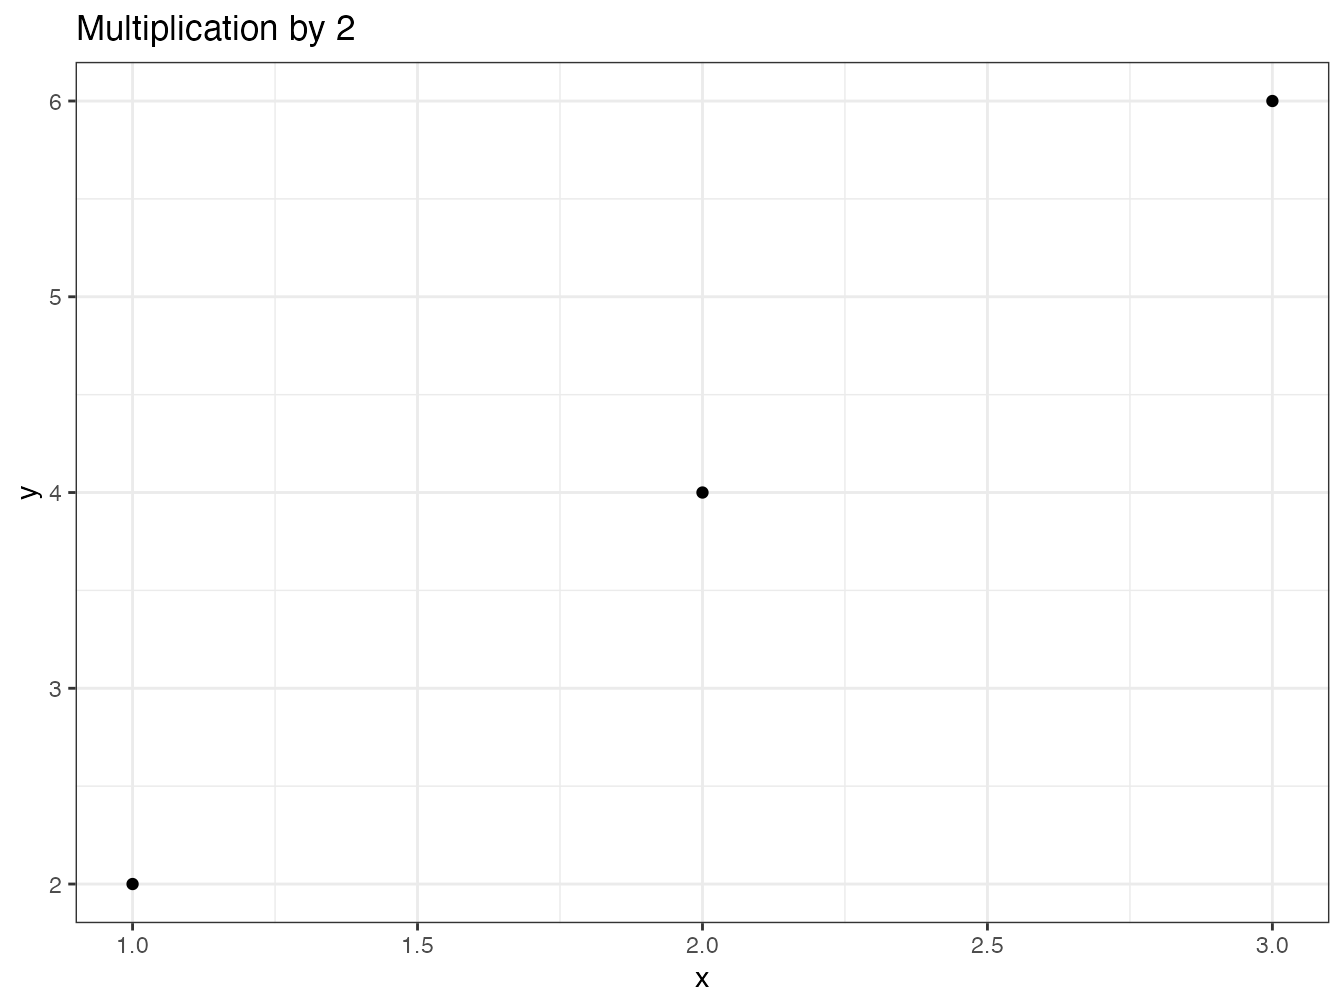
\includegraphics[width=0.8\linewidth]{travailleR_files/figure-latex/plot.multiple-2} \end{center}

\normalsize

Pour des raisons techniques liées à l'évaluation non conventionnelle dans le tidyverse, les noms de variables utilisées par \texttt{aes()} doivent être préfixées par \texttt{.data\$} dans les packages et \texttt{rlang::.data} doit être importé.
Dans le cas contraire, la vérification du package renvoie une note indiquant que les variables \texttt{x} et \texttt{y}, utilisées par les arguments de \texttt{aes()} n'ont pas été déclarées et n'existent peut-être pas dans l'environnement local (voir section \ref{sec:environnements}).

\subsubsection{Documentation}\label{documentation}

Les méthodes génériques et les fonctions qui les déclinent doivent être documentées comme n'importe quelle autre fonction.

La gestion de l'espace des noms est un peu plus complexe:

\begin{itemize}
\tightlist
\item
  Les méthodes génériques doivent être exportées:
\end{itemize}

\begin{verbatim}
#' @export
\end{verbatim}

\begin{itemize}
\tightlist
\item
  Les fonctions dérivées de méthodes génériques ne doivent pas être exportées mais être déclarées comme méthodes, avec le nom de la méthode générique et la classe traitée.
  \textbf{roxygen2} demande qu'une directive d'exportation soit ajoutée mais ne l'applique pas (comme il se doit) dans le fichier \texttt{NAMESPACE} qui est utilisé par R:
\end{itemize}

\begin{verbatim}
#' @method plot multiple
#' @export
\end{verbatim}

\begin{itemize}
\tightlist
\item
  Depuis la version 3 de \textbf{roxygen2}, la déclaration \texttt{@method} est inutile tant que le nom de la fonction est décomposable sans ambiguïté, comme \texttt{plot.multiple}: \texttt{@export} suffit.
  Si le nom de la fonction dérivée comporte plusieurs points, \textbf{roxygen2} peut ne pas détecter automatiquement le générique et l'objet et \texttt{@method} doit être maintenu.
\item
  Les fonctions dérivées de méthodes génériques venant d'un autre package nécessitent d'importer la méthode générique, sauf si elle est fournie par \textbf{base} (\texttt{print} est fourni par \textbf{base} et n'est donc pas concerné):
\end{itemize}

\begin{verbatim}
#' @importFrom graphics plot
#' @importFrom ggplot2 autoplot
\end{verbatim}

\begin{itemize}
\tightlist
\item
  Les génériques importés de cette manière doivent être réexportés par une directive à placer par exemple juste après le code de la fonction dérivée:
\end{itemize}

\begin{verbatim}
#' @export
graphics::plot

#' @export
ggplot2::autoplot
\end{verbatim}

\begin{itemize}
\tightlist
\item
  \textbf{roxygen2} crée automatiquement un fichier d'aide \texttt{reexports.Rd} dans lequel se trouve un lien vers la documentation originale des génériques réexportés.
\end{itemize}

Dans \texttt{DESCRIPTION}, le package d'origine de chaque générique doit être listé dans la directive \texttt{Imports:}:

\begin{verbatim}
Imports: ggplot2, graphics
\end{verbatim}

Enfin, l'importation de fonctions du tidyverse nécessite aussi quelques précautions:

\begin{itemize}
\tightlist
\item
  le package \textbf{tidyverse} est réservé à l'usage interactif de R: il n'est pas question de l'importer dans \texttt{DESCRIPTION} parce que ses dépendances peuvent changer et aboutir à des résultats imprévisibles.
  Le package \textbf{magrittr} fournit les tuyaux, principalement \texttt{\%\textgreater{}\%}.
  Le package \textbf{rlang} fournit l'objet \texttt{.data} présenté ci-dessous.
  Il doivent être importés dans \texttt{DESCRIPTION}.
\end{itemize}

\begin{verbatim}
Imports: magrittr, rlang, stats
\end{verbatim}

\begin{itemize}
\tightlist
\item
  Comme il n'est pas possible de préfixer les \texttt{\%\textgreater{}\%} par le nom du package, il faut importer la fonction en utilisant les délimiteurs prévus pour les fonctions dont le nom contient des caractères spéciaux:
\end{itemize}

\scriptsize

\begin{Shaded}
\begin{Highlighting}[]
\CommentTok{\#\textquotesingle{} @importFrom magrittr \textasciigrave{}\%\textgreater{}\%\textasciigrave{}}
\end{Highlighting}
\end{Shaded}

\normalsize

\begin{itemize}
\tightlist
\item
  Les fonctions du tidyverse qui utilisent des noms de colonnes de tibbles ou dataframes génèrent des avertissements au moment de la vérification du package parce que ces noms sont confondus avec des noms de variables non définies.
  Pour éviter cette confusions, l'objet \texttt{.data} du package \textbf{rlang} est utilisé (par exemple dans \texttt{aes()} vu plus haut).
  Il doit être importé:
\end{itemize}

\scriptsize

\begin{Shaded}
\begin{Highlighting}[]
\CommentTok{\#\textquotesingle{} @importFrom rlang .data}
\end{Highlighting}
\end{Shaded}

\normalsize

Finalement, le code complet est le suivant:

\scriptsize

\begin{Shaded}
\begin{Highlighting}[]
\CommentTok{\#\textquotesingle{} Multiplication of a numeric vector}
\CommentTok{\#\textquotesingle{}}
\CommentTok{\#\textquotesingle{} @param number a numeric vector}
\CommentTok{\#\textquotesingle{} @param times a number to multiply}
\CommentTok{\#\textquotesingle{}}
\CommentTok{\#\textquotesingle{} @return an object of class \textasciigrave{}multiple\textasciigrave{}}
\CommentTok{\#\textquotesingle{} @export}
\CommentTok{\#\textquotesingle{}}
\CommentTok{\#\textquotesingle{} @examples}
\CommentTok{\#\textquotesingle{} multiple(1:2,3)}
\NormalTok{multiple }\OtherTok{\textless{}{-}} \ControlFlowTok{function}\NormalTok{(number, }\AttributeTok{times =} \DecValTok{1}\NormalTok{) \{}
  \CommentTok{\# Calculate the multiples}
\NormalTok{  y }\OtherTok{\textless{}{-}}\NormalTok{ number }\SpecialCharTok{*}\NormalTok{ times}
  \CommentTok{\# Save in a list}
\NormalTok{  result }\OtherTok{\textless{}{-}} \FunctionTok{list}\NormalTok{(}\AttributeTok{x =}\NormalTok{ number, }\AttributeTok{y =}\NormalTok{ y, }\AttributeTok{times =}\NormalTok{ times)}
  \CommentTok{\# Set the class}
  \FunctionTok{class}\NormalTok{(result) }\OtherTok{\textless{}{-}} \FunctionTok{c}\NormalTok{(}\StringTok{"multiple"}\NormalTok{, }\FunctionTok{class}\NormalTok{(result))}
  \FunctionTok{return}\NormalTok{(result)}
\NormalTok{\}}

\CommentTok{\#\textquotesingle{} Print objects of class multiple}
\CommentTok{\#\textquotesingle{}}
\CommentTok{\#\textquotesingle{} @param x an object of class \textasciigrave{}multiple\textasciigrave{}.}
\CommentTok{\#\textquotesingle{} @param ... further arguments passed to the generic method.}
\CommentTok{\#\textquotesingle{}}
\CommentTok{\#\textquotesingle{} @export}
\CommentTok{\#\textquotesingle{}}
\CommentTok{\#\textquotesingle{} @examples}
\CommentTok{\#\textquotesingle{} print(multiple(2,3))}
\NormalTok{print.multiple }\OtherTok{\textless{}{-}} \ControlFlowTok{function}\NormalTok{(x, ...) \{}
  \FunctionTok{print.default}\NormalTok{(x}\SpecialCharTok{$}\NormalTok{y)}
\NormalTok{\}}

\CommentTok{\#\textquotesingle{} Summarize objects of class multiple}
\CommentTok{\#\textquotesingle{}}
\CommentTok{\#\textquotesingle{} @param object an object of class \textasciigrave{}multiple\textasciigrave{}.}
\CommentTok{\#\textquotesingle{} @param ... further arguments passed to the generic method.}
\CommentTok{\#\textquotesingle{}}
\CommentTok{\#\textquotesingle{} @export}
\CommentTok{\#\textquotesingle{}}
\CommentTok{\#\textquotesingle{} @examples}
\CommentTok{\#\textquotesingle{} summary(multiple(2,3))}
\NormalTok{summary.multiple }\OtherTok{\textless{}{-}} \ControlFlowTok{function}\NormalTok{(object, ...) \{}
  \FunctionTok{print.default}\NormalTok{(object}\SpecialCharTok{$}\NormalTok{x)}
  \FunctionTok{cat}\NormalTok{(}\StringTok{"multiplied by"}\NormalTok{, object}\SpecialCharTok{$}\NormalTok{times, }\StringTok{"is:}\SpecialCharTok{\textbackslash{}n}\StringTok{"}\NormalTok{)}
  \FunctionTok{print.default}\NormalTok{(object}\SpecialCharTok{$}\NormalTok{y)}
\NormalTok{\}}

\CommentTok{\#\textquotesingle{} Plot objects of class multiple}
\CommentTok{\#\textquotesingle{}}
\CommentTok{\#\textquotesingle{} @param x a vector of numbers}
\CommentTok{\#\textquotesingle{} @param y a vector of multiplied numbers}
\CommentTok{\#\textquotesingle{} @param ... further arguments passed to the generic method.}
\CommentTok{\#\textquotesingle{}}
\CommentTok{\#\textquotesingle{} @importFrom graphics plot}
\CommentTok{\#\textquotesingle{} @export}
\CommentTok{\#\textquotesingle{}}
\CommentTok{\#\textquotesingle{} @examples}
\CommentTok{\#\textquotesingle{} plot(multiple(2,3))}
\NormalTok{plot.multiple }\OtherTok{\textless{}{-}} \ControlFlowTok{function}\NormalTok{(x, y, ...) \{}
  \FunctionTok{plot.default}\NormalTok{(}
    \AttributeTok{x =}\NormalTok{ x}\SpecialCharTok{$}\NormalTok{x, }
    \AttributeTok{y =}\NormalTok{ x}\SpecialCharTok{$}\NormalTok{y, }
    \AttributeTok{type =} \StringTok{"p"}\NormalTok{, }
    \AttributeTok{main =} \FunctionTok{paste}\NormalTok{(}\StringTok{"Multiplication by"}\NormalTok{, x}\SpecialCharTok{$}\NormalTok{times), }
\NormalTok{    ...}
\NormalTok{  )}
\NormalTok{\}}
\CommentTok{\#\textquotesingle{} @export}
\NormalTok{graphics}\SpecialCharTok{::}\NormalTok{plot}
\end{Highlighting}
\end{Shaded}

\begin{verbatim}
## function (x, y, ...) 
## UseMethod("plot")
## <bytecode: 0x133742b10>
## <environment: namespace:base>
\end{verbatim}

\begin{Shaded}
\begin{Highlighting}[]
\CommentTok{\#\textquotesingle{} autoplot}
\CommentTok{\#\textquotesingle{}}
\CommentTok{\#\textquotesingle{} ggplot of the \textasciigrave{}multiple\textasciigrave{} objects.}
\CommentTok{\#\textquotesingle{}}
\CommentTok{\#\textquotesingle{} @param object an object of class \textasciigrave{}multiple\textasciigrave{}.}
\CommentTok{\#\textquotesingle{} @param ... ignored.}
\CommentTok{\#\textquotesingle{}}
\CommentTok{\#\textquotesingle{} @return a \textasciigrave{}ggplot\textasciigrave{} object}
\CommentTok{\#\textquotesingle{} @importFrom ggplot2 autoplot}
\CommentTok{\#\textquotesingle{} @importFrom magrittr \textasciigrave{}\%\textgreater{}\%\textasciigrave{}}
\CommentTok{\#\textquotesingle{} @importFrom rlang .data}
\CommentTok{\#\textquotesingle{} @export}
\CommentTok{\#\textquotesingle{}}
\CommentTok{\#\textquotesingle{} @examples}
\CommentTok{\#\textquotesingle{} autoplot(multiple(2,3))}
\NormalTok{autoplot.multiple }\OtherTok{\textless{}{-}} \ControlFlowTok{function}\NormalTok{(object, ...) \{}
  \FunctionTok{data.frame}\NormalTok{(}\AttributeTok{x =}\NormalTok{ object}\SpecialCharTok{$}\NormalTok{x, }\AttributeTok{y =}\NormalTok{ object}\SpecialCharTok{$}\NormalTok{y) }\SpecialCharTok{\%\textgreater{}\%}
\NormalTok{    ggplot2}\SpecialCharTok{::}\FunctionTok{ggplot}\NormalTok{() }\SpecialCharTok{+}
\NormalTok{    ggplot2}\SpecialCharTok{::}\FunctionTok{geom\_point}\NormalTok{(ggplot2}\SpecialCharTok{::}\FunctionTok{aes}\NormalTok{(}\AttributeTok{x =}\NormalTok{ .data}\SpecialCharTok{$}\NormalTok{x, }\AttributeTok{y =}\NormalTok{ .data}\SpecialCharTok{$}\NormalTok{y)) }\SpecialCharTok{+}
\NormalTok{    ggplot2}\SpecialCharTok{::}\FunctionTok{labs}\NormalTok{(}\AttributeTok{title =} \FunctionTok{paste}\NormalTok{(}\StringTok{"Multiplication by"}\NormalTok{, object}\SpecialCharTok{$}\NormalTok{times))}
\NormalTok{\}}
\CommentTok{\#\textquotesingle{} @export}
\NormalTok{ggplot2}\SpecialCharTok{::}\NormalTok{autoplot}
\end{Highlighting}
\end{Shaded}

\begin{verbatim}
## function (object, ...) 
## {
##     UseMethod("autoplot")
## }
## <bytecode: 0x131348940>
## <environment: namespace:ggplot2>
\end{verbatim}

\normalsize

\subsection{Code C++}\label{code-c}

L'utilisation de code C++ a été vue en section \ref{sec:cpp}.
Pour intégrer ces fonctions dans un packages, il faut respecter les règles suivantes:

\begin{itemize}
\tightlist
\item
  les fichiers \texttt{.cpp} contenant le code sont placés dans le dossier \texttt{/src} du projet;
\item
  le code est commenté pour \textbf{roxygen2} de la même façon que les fonctions R, mais avec le marqueur de commentaire du langage C:
\end{itemize}

\scriptsize

\begin{Shaded}
\begin{Highlighting}[]
\PreprocessorTok{\#include }\ImportTok{\textless{}Rcpp.h\textgreater{}}
\KeywordTok{using} \KeywordTok{namespace}\NormalTok{ Rcpp}\OperatorTok{;}

\CommentTok{//\textquotesingle{} timesTwo}
\CommentTok{//\textquotesingle{}}
\CommentTok{//\textquotesingle{} Calculates the double of a value.}
\CommentTok{//\textquotesingle{}}
\CommentTok{//\textquotesingle{} @param x A numeric vector.}
\CommentTok{//\textquotesingle{} @export}
\CommentTok{// [[Rcpp::export]]}
\NormalTok{NumericVector timesTwo}\OperatorTok{(}\NormalTok{NumericVector x}\OperatorTok{)} \OperatorTok{\{}
  \ControlFlowTok{return}\NormalTok{ x }\OperatorTok{*} \DecValTok{2}\OperatorTok{;}
\OperatorTok{\}}
\end{Highlighting}
\end{Shaded}

\normalsize

\begin{itemize}
\tightlist
\item
  dans \texttt{DESCRIPTION}, importer les packages.
  \textbf{Rcpp}, et \textbf{RcppParallel} si du code parallélisé est utilisé (supprimer ses références sinon), doivent être déclarés dans \texttt{LinkingTo}:
\end{itemize}

\begin{verbatim}
Imports: Rcpp, RcppParallel
LinkingTo: Rcpp, RcppParallel
\end{verbatim}

\begin{itemize}
\tightlist
\item
  les commentaires pour \textbf{roxygen2} doivent être ajoutés à \texttt{package.R} (\enquote{multiple} est le nom du package):
\end{itemize}

\scriptsize

\begin{Shaded}
\begin{Highlighting}[]
\CommentTok{\#\textquotesingle{} @importFrom Rcpp sourceCpp}
\CommentTok{\#\textquotesingle{} @importFrom RcppParallel RcppParallelLibs}
\CommentTok{\#\textquotesingle{} @useDynLib multiple, .registration = TRUE}
\end{Highlighting}
\end{Shaded}

\normalsize

\begin{itemize}
\tightlist
\item
  les fichiers de travail de C++ sont exclus du contrôle de source dans \texttt{.gitignore}:
\end{itemize}

\begin{verbatim}
# C binaries
src/*.o
src/*.so
src/*.dll
\end{verbatim}

Ces modifications sont en partie effectuées automatiquement, pour \textbf{Rcpp} seulement, par \textbf{usethis}, mais l'insertion manuelle du code est plus rapide et fiable: ne pas utiliser cette commande.

\scriptsize

\begin{Shaded}
\begin{Highlighting}[]
\CommentTok{\# usethis::use\_rcpp()}
\end{Highlighting}
\end{Shaded}

\normalsize

La construction du package entraînera la compilation du code: les Rtools sont donc indispensables.

\subsection{Package bien rangé}\label{package-bien-ranguxe9}

Tout package moderne doit être compatible avec le tidyverse, ce qui nécessite peu d'efforts:

\begin{itemize}
\tightlist
\item
  pour permettre l'utilisation de pipelines, l'argument principal des fonctions doit être le premier;
\item
  les fonctions qui transforment des données doivent accepter un dataframe ou un tibble comme premier argument et retourner un objet du même format;
\item
  les méthodes \texttt{plot()} doivent être doublées de méthodes \texttt{autoplot()} avec les mêmes arguments qui produisent le même graphique avec \textbf{ggplot2}.
\end{itemize}

\section{Bibliographie}\label{bibliographie-1}

La documentation d'un package fait appel à des références bibliographiques.
Elles peuvent être gérées automatiquement avec \textbf{Rdpack} et \textbf{roxygen2}.
Les références utilisées dans les fichiers R Markdown (vignette, site produit par \textbf{pkgdown}) ne sont pas concernées.

\subsection{Préparation}\label{pruxe9paration}

Les références bibliographiques doivent être placées dans un fichier BibTeX \texttt{REFERENCES.bib} placé dans le dossier \texttt{inst}.
Ce dossier contient des fichiers qui seront placés à la racine du dossier du package quand il sera installé.

Ajouter la ligne suivante à \texttt{DESCRIPTION}:

\begin{verbatim}
RdMacros: Rdpack
\end{verbatim}

Ajouter aussi le package \texttt{Rdpack} à la liste des packages importés:

\begin{verbatim}
Imports: magrittr, stats, Rcpp, Rdpack
\end{verbatim}

Enfin, importer la fonction \texttt{reprompt()} de \textbf{Rdpack} en ajoutant les lignes suivantes à la documentation pour \textbf{roxygen2} dans \texttt{package.R}:

\scriptsize

\begin{Shaded}
\begin{Highlighting}[]
\CommentTok{\#\textquotesingle{} @importFrom Rdpack reprompt}
\end{Highlighting}
\end{Shaded}

\normalsize

\subsection{Citations}\label{citations}

Les références sont citées par la commande \texttt{\textbackslash{}insertCite\{key\}\{package\}} dans la documentation destinée à \textbf{roxygen2}.
\texttt{package} est le nom du package dans lequel le fichier \texttt{REFERENCES.bib} doit être cherché: ce sera normalement le package en cours, mais les références d'autres packages sont accessibles, à la seule condition qu'ils utilisent \textbf{Rdpack}.

\texttt{key} est l'identifiant de la référence dans le fichier.
Exemple\footnote{Package \textbf{divent} sur GitHub: \url{https://github.com/EricMarcon/divent/blob/master/R/package.R}}: documentation du package \textbf{divent} hébergé sur GitHub, fichier \texttt{.R} du package:

\scriptsize

\begin{Shaded}
\begin{Highlighting}[]
\CommentTok{\#\textquotesingle{} divent}
\CommentTok{\#\textquotesingle{}}
\CommentTok{\#\textquotesingle{} Measures of Diversity and Entropy}
\CommentTok{\#\textquotesingle{} }
\CommentTok{\#\textquotesingle{} This package is a reboot of the **entropart** package \textbackslash{}insertCite\{Marcon2014c\}\{divent\}.}
\CommentTok{\#\textquotesingle{}}
\CommentTok{\#\textquotesingle{} @importFrom Rdpack reprompt}
\CommentTok{\#\textquotesingle{} }
\CommentTok{\#\textquotesingle{} @references}
\CommentTok{\#\textquotesingle{} \textbackslash{}insertAllCited\{\}}
\StringTok{"\_PACKAGE"}
\end{Highlighting}
\end{Shaded}

\begin{verbatim}
## [1] "_PACKAGE"
\end{verbatim}

\normalsize

La référence citée se trouve dans \texttt{inst/REFERENCES.bib}:

\begin{verbatim}
@Article{Marcon2014c,
  author  = {Marcon, Eric and Herault, Bruno},
  title   = {entropart, an R Package to Partition 
             Diversity},
  journal = {Journal of Statistical Software},
  year    = {2015},
  volume  = {67},
  number  = {8},
  pages   = {1--26},
}
\end{verbatim}

Les citations sont entre parenthèses.
Pour placer le nom de l'auteur hors de la parenthèse, ajouter la déclaration \texttt{;textual}:

\begin{verbatim}
\insertCite{Marcon2014c;textual}{divent}
\end{verbatim}

Pour citer plusieurs références (forcément du même package), les séparer par des virgules.

A la fin de la documentation d'un objet utilisant des citations, ajouter systématiquement une liste des références:

\scriptsize

\begin{Shaded}
\begin{Highlighting}[]
\CommentTok{\#\textquotesingle{} @references}
\CommentTok{\#\textquotesingle{} \textbackslash{}insertAllCited\{\}}
\end{Highlighting}
\end{Shaded}

\normalsize

\section{Données}\label{donnuxe9es}

Des données peuvent être intégrées à un package, notamment pour la clarté des exemples.

La méthode la plus simple consiste à utiliser \textbf{usethis}.
Créer des variables contenant les données à sauvegarder puis les sauvegarder:

\scriptsize

\begin{Shaded}
\begin{Highlighting}[]
\NormalTok{seq1\_10 }\OtherTok{\textless{}{-}} \DecValTok{1}\SpecialCharTok{:}\DecValTok{10}
\NormalTok{seq1\_100 }\OtherTok{\textless{}{-}} \DecValTok{1}\SpecialCharTok{:}\DecValTok{100}
\NormalTok{usethis}\SpecialCharTok{::}\FunctionTok{use\_data}\NormalTok{(seq1\_10, seq1\_100)}
\end{Highlighting}
\end{Shaded}

\normalsize

Un fichier \texttt{.rda} est créé dans le dossier \texttt{data} pour chaque variable créée.
Avec l'option \texttt{LazyData} activée dans \texttt{DESCRIPTION}, les variables seront disponibles dès le chargement du package, mais ne seront effectivement chargées en mémoire qu'après leur première utilisation.

Chaque variable doit être documentée dans le fichier \texttt{package.R}:

\scriptsize

\begin{Shaded}
\begin{Highlighting}[]
\CommentTok{\#\textquotesingle{} seq1\_10}
\CommentTok{\#\textquotesingle{}}
\CommentTok{\#\textquotesingle{} A sequence of numbers from 1 to 10}
\CommentTok{\#\textquotesingle{}}
\CommentTok{\#\textquotesingle{} @format A numeric vector.}
\CommentTok{\#\textquotesingle{} @source Values computed by the R software, }
\CommentTok{\#\textquotesingle{}   \textbackslash{}url\{https://www.r{-}project.org/\}}
\StringTok{"seq1\_10"}
\end{Highlighting}
\end{Shaded}

\normalsize

Le nom de la variable est donné entre guillemets après le bloc de commentaires (à la place du code R d'une fonction).
\texttt{@format} décrit le format des données et \texttt{@source} permet d'indiquer leur source.

\section{Tests unitaires}\label{tests-unitaires}

Dans l'idéal, tout le code inclus dans un package devrait être testé de multiples façons:

\begin{itemize}
\tightlist
\item
  contre les erreurs de syntaxe: les procédures de vérification de R s'en chargent assez bien;
\item
  pour vérifier la conformité des résultats de calculs aux valeurs attendues;
\item
  contre la survenue d'erreurs si les utilisateurs n'utilisent pas le code comme le développeur l'a prévu (arguments incorrects passés aux fonctions, données inadéquates\ldots).
\end{itemize}

Les tests unitaires sont utilisés dans les deux derniers objectifs.
Ils s'appuient sur \textbf{testthat} à intégrer au package:

\scriptsize

\begin{Shaded}
\begin{Highlighting}[]
\NormalTok{usethis}\SpecialCharTok{::}\FunctionTok{use\_testthat}\NormalTok{()}
\end{Highlighting}
\end{Shaded}

\normalsize

\scriptsize

\normalsize

Les tests doivent être ajoutés sous la forme de fichiers \texttt{.R} dont le nom commence obligatoirement par \texttt{test} dans le dossier \texttt{tests/testthat}.

Chaque test (donc le contenu de chaque fichier) commence par son contexte, c'est-à-dire ce un ensemble de tests. Exemple, dans un fichier \texttt{test\_double.R}:

\scriptsize

\begin{Shaded}
\begin{Highlighting}[]
\FunctionTok{context}\NormalTok{(}\StringTok{"function double"}\NormalTok{)}
\end{Highlighting}
\end{Shaded}

\normalsize

Les tests sont contenus dans des fichiers qui les regroupent par thème, par exemple \texttt{test\_double.R}.
Le nom de chaque test est passé comme argument de la fonction \texttt{test\_that()}:

\scriptsize

\begin{Shaded}
\begin{Highlighting}[]
\FunctionTok{test\_that}\NormalTok{(}\StringTok{"Double values are correct"}\NormalTok{, \{}
  \FunctionTok{skip\_on\_cran}\NormalTok{()}

\NormalTok{  x }\OtherTok{\textless{}{-}} \DecValTok{1}\SpecialCharTok{:}\DecValTok{2}

  \CommentTok{\# 2 x 2 should be 4}
  \FunctionTok{expect\_equal}\NormalTok{(}\FunctionTok{double}\NormalTok{(x), }\FunctionTok{c}\NormalTok{(}\DecValTok{2}\NormalTok{, }\DecValTok{4}\NormalTok{))}
  \CommentTok{\# The result should be a number (type = "double")}
  \FunctionTok{expect\_type}\NormalTok{(}\FunctionTok{double}\NormalTok{(x), }\StringTok{"double"}\NormalTok{)}
  \CommentTok{\# Error management}
  \FunctionTok{expect\_error}\NormalTok{(}\FunctionTok{double}\NormalTok{(}\StringTok{"a"}\NormalTok{))}
\NormalTok{\})}
\end{Highlighting}
\end{Shaded}

\begin{verbatim}
## Test passed
\end{verbatim}

\normalsize

Toutes les fonctions commençant par \texttt{expect} permettent de comparer leur premier argument à un résultat: dans l'exemple ci-dessus, le résultat de \texttt{double(1:2)} doit être \texttt{2\ 4} et le type de ce vecteur doit être réel à double précision.
Le dernier test vérifie qu'une chaîne de caractère passée comme argument génère une erreur, ce qui n'est pas optimal: si le package traitait l'erreur, le message retourné pourrait être testé.

La commande \texttt{skip\_on\_cran()}, à utiliser systématiquement, évite de lancer les tests sur CRAN quand le package y sera déposé: CRAN dispose de ressources limitées et restreint strictement le temps de vérification des packages sur sa plateforme.
Les tests devront donc être réalisés sur GitHub, grâce à l'intégration continue, voir section \ref{sec:package-ci5}.

Les tests peuvent être lancés par le menu \enquote{More \textgreater{} Test package} de la fenêtre \emph{Build} ou par la commande \texttt{devtools::test()}.

Il est conseillé d'écrire les tests dès qu'une fonction du package est stabilisée.

\section{Fichier .gitignore}\label{fichier-.gitignore}

Le fichier \texttt{.gitignore} obtenu à ce stade est incomplet.
Il peut être remplacé par celui-ci:

\begin{verbatim}
# History files
.Rhistory
.Rapp.history
# Session Data files
.RData
# Example code in package build process
*-Ex.R
# Output files from R CMD build
/*.tar.gz
# Output files from R CMD check
/*.Rcheck/
# RStudio files
.Rproj.user/
.Rprofile
# knitr and R markdown default cache directories
*_cache/
/cache/
# Temporary files created by R markdown
*.utf8.md
*.knit.md
# C binaries
src/*.o
src/*.so
src/*.dll
/src-i386/
/src-x64/
# uncomment if pkgdown is run by CI
# docs/
\end{verbatim}

La dernière ligne concerne le dossier \texttt{docs/}, qui reçoit le site web produit par \textbf{pkgdown}.
Elle est commentée tant que la production du site est réalisée localement, mais décommentée si elle est confiée à GitHub Actions (voir section suivante).

\section{Intégration continue}\label{sec:package-ci5}

La vérification (\emph{Check}) du package doit être effectuée à chaque étape du développement, ce qui consomme un temps considérable.
Elle peut être automatisée très simplement avec le service GitHub Actions, déclenché à chaque modification du dépôt sur GitHub.
L'analyse de la couverture du code par les tests (quelles parties du codes sont testées ou non) sera ajoutée.

GitHub est également capable de reconstruire la documentation du package avec \textbf{pkgdown}, autre opération consommatrice de ressources, après la réussite des tests.

La section \ref{sec:package-ci6} détaille le moyen de le faire.

\section{CRAN}\label{sec:package-cran}

Les packages dont l'audience dépasse l'entourage de l'auteur peuvent être déposés sur CRAN.
Les règles à respecter sur CRAN sont nombreuses\footnote{\url{https://cran.r-project.org/web/packages/policies.html}}. Elles sont vérifiées par la commande de vérification \texttt{R\ CMD\ check} avec l'option \texttt{-\/-\ as.cran}.
La vérification ne doit renvoyer aucune erreur, aucun avertissement, ni aucune note avant de soumettre le package.

\subsection{Test du package}\label{test-du-package}

La vérification du package par GitHub dans le cadre de l'intégration continue n'est pas suffisante.
Le package doit être testé sur la version de développement de R.
Le site \emph{R-hub builder}\footnote{\url{https://builder.r-hub.io/}} permet de le faire simplement.

Le package, dont la version ne doit pas être de développement (limitée à trois nombres, voir section \ref{sec:package-description}), doit être construit au format source: dans la fenêtre \emph{Build} de RStudio, cliquer sur \enquote{More \textgreater{} Build Source Package}.
Sur le site \emph{R-hub builder}, cliquer sur \enquote{Advanced}, sélectionner le fichier source du package et la plateforme de test: \emph{Debian Linux, R-devel, GCC}.

Le package \textbf{rhub} permet d'utiliser la même plateforme de vérification que le site \emph{R-hub builder} depuis RStudio.
La première étape consiste à valider son adresse de messagerie avec la commande \texttt{validate\_email()}.
Ensuite, il suffit d'appeler la fonction \texttt{check\_for\_cran()} pour lancer une vérification complète.

\subsection{Soumission}\label{soumission}

Quand le package est au point, la soumission à CRAN se fait par le site web dédié\footnote{\url{https://xmpalantir.wu.ac.at/cransubmit/}}.

En cas de rejet, traiter les demandes et soumettre à nouveau en incrémentant le numéro de version.

\subsection{Maintenance}\label{maintenance}

Des demandes de corrections sont envoyées par CRAN de temps à autre, notamment lors des changements de version de R.
L'adresse de messagerie du responsable du package (\emph{maintainer}) doit rester valide et les demandes doivent être traitées rapidement.
Dans le cas contraire, le package est archivé.

Les nouvelles versions du package sont soumises de la même façon que la première.

\chapter{Intégration continue}\label{chap-ci}

\toc{1}

L'intégration continue consiste à confier à un service externe la tâche de vérifier un package, produire des documents Markdown pour les pages web d'un dépôt GitHub ou tricoter entièrement un site web à partir du code.

Toutes ces tâches peuvent être accomplies localement sur le poste de travail mais prennent du temps et risquent de ne pas être répétées à chaque mise à jour.
Dans le cadre de l'intégration continue, elles le sont systématiquement, de façon transparente pour l'utilisateur.
En cas d'échec, un message d'alerte est envoyé.

La mise en place de l'intégration continue se justifie pour des projets lourds, avec des mises à jour régulières.
plutôt que pour des projets contenant un simple document Markdown rarement modifié.

\section{Outils}\label{outils}

\subsection{GitHub Actions}\label{github-actions}

L'outil utilisé le plus fréquemment pour des projets R déposés sur GitHub était \emph{Travis CI}\footnote{\url{https://travis-ci.org/}} mais le service est devenu payant en 2021.

Les Actions GitHub remplacent avantageusement Travis.
Ce service est intégré à GitHub.

\subsection{Codecov}\label{codecov}

Pour évaluer le taux de couverture du code des packages R, c'est-à-dire la proportion du code testé d'une façon ou d'une autre (exemples, tests unitaires, vignette), le service \emph{Codecov}\footnote{\url{https://codecov.io/}} s'intègre parfaitement à GitHub.

Il faut ouvrir un compte, de préférence en s'authentifiant par GitHub.

\subsection{GitHub Pages}\label{github-pages}

Les pages web de GitHub peuvent être hébergées dans le répertoire \texttt{docs} de la branche master du projet: c'est la solution retenue quand elle sont produites sur le poste de travail.

Si elles sont produites par intégration continue, elle le seront obligatoirement dans une branche dédiée appelée \texttt{gh-pages}.

\section{Principes}\label{principes}

Un projet de document est traité en exemple.
L'objectif est de faire tricoter par GitHub un projet Markdown.
Cette pratique est appropriée pour les projets d'ouvrages, qui nécessitent beaucoup de ressources pour leur construction.
Dans ce type de projet, le code est tricoté par \textbf{knitr} pour produire plusieurs documents, typiquement aux formats HTML et PDF, accessibles sur les pages GitHub.
Quand les documents sont produits localement, ils sont placés dans le dossier \texttt{docs} et poussés sur GitHub.

Pour que GitHub s'en charge, quelques réglages sont nécessaires.

\subsection{Obtention d'un jeton d'accès personnel}\label{obtention-dun-jeton-daccuxe8s-personnel}

Pour écrire sur GitHub, le service d'intégration continue devra s'authentifier au moyen d'un jeton d'accès personnel (\emph{Personal Access Token}: PAT) dont la création est décrite en section \ref{sec:pat}.

Générer un nouveau jeton, le décrire en tant que \enquote{GitHub Actions} et lui donner les autorisations:

\begin{itemize}
\tightlist
\item
  \enquote{repo}, c'est-à-dire modifier \emph{tous} les dépôts (il n'est pas possible de limiter l'accès à un dépôt particulier).
\item
  \enquote{workflow}, c'est-à-dire exécuter lles scripts d'intégration continue.
\end{itemize}

\subsection{Secrets du projet}\label{sec:secrets-ci}

Sur GitHub, afficher les paramètres du projet et sélectionner \enquote{Secrets}.
Le bouton \enquote{New Repository Secret} permet de stocker des variables utilisées dans les scripts des Actions GitHub (visibles publiquement) sans en diffuser la valeur.
Le jeton d'accès personnel est indispensable pour que les Actions GitHub puissent écrire leur production dans le projet.
Créer un secret nommé \enquote{GH\_PAT} et saisir la valeur du jeton sauvegardée précédemment.
Après avoir cliqué sur \enquote{Add Secret}, le jeton ne pourra plus être lu.

Pour permettre l'envoi de messages de succès ou d'échec sans diffuser son adresse de messagerie, créer un secret nommé \enquote{EMAIL} qui la contient.

\subsection{Activation du dépôt sur CodeCov}\label{activation-du-duxe9puxf4t-sur-codecov}

L'analyse de la couverture du code des packages est utile pour détecter les portions de code non testées.
En revanche, l'analyse de la couverture des projets de document n'a pas d'intérêt.

Pour activer un dépôt, il faut d'authentifier sur le site de CodeCov avec son compte GitHub.
La liste des dépôts est affichée et peut être actualisée.
Si les dépôts à traiter sont hébergés par une organisation, par exemple les dépôts d'une salle de classe GitHub, il faut actualiser la liste des organisations en suivant les instructions (un lien permet de modifier rapidement les options de GitHub pour autoriser la lecture d'une organisation par Codecov) et à nouveau mettre à jour la liste des dépôts.
Enfin, quand le dépôt recherché est visible, il faut l'activer.
Il est inutile d'utiliser le système de jetons de Codecov.

\subsection{Scripter les actions de GitHub}\label{scripter-les-actions-de-github}

Un flux de travail (\emph{workflow}) de GitHub est une succession de tâches (\emph{jobs}) comprenant des étapes (\emph{steps}).
Un flux de travail est déclenché par un évènement, généralement chaque \emph{push} du projet, mais aussi à intervalles réguliers (\emph{cron}).

Typiquement, les flux créés ici contiennent deux tâches: la première installe R et les composants nécessaires et exécute des scripts R (ce qui constitue ses étapes successives); la seconde publie des fichiers obtenus dans les pages GitHub.

Les flux de travail sont configurés dans un fichier au format YAML placé dans le dossier \texttt{.github/workflows/} du projet.
Les différentes parties du script sont présentées ci-dessous.
Le script complet est celui de ce document, accessible sur GitHub\footnote{\url{https://github.com/EricMarcon/travailleR/blob/master/.github/workflows/bookdown.yml}}.

\subsubsection{Déclenchement}\label{sec:declenchement}

L'action est déclenchée à chaque fois que des mises à jour sont poussées sur GitHub:

\begin{verbatim}
on:
  push:
     branches:
       - master
\end{verbatim}

La branche prise en compte est \emph{master} (à remplacer par \emph{main} le cas échéant).

Pour déclencher l'action périodiquement, il faut utiliser la syntaxe de \emph{cron} (le système de planification des tâches sous Unix):

\begin{verbatim}
on:
  schedule:
    - cron: '0 22 * * 0'  # every sunday at 22:00
\end{verbatim}

Les valeurs successives sont celles des minutes, des heures, du jour (quantième du mois), du mois et du jour de la semaine (0 pour dimanche à 6 pour samedi).
Les \texttt{*} permettent d'ignorer une valeur.

Les entrées \texttt{push} et \texttt{schedule} peuvent être utilisées ensemble:

\begin{verbatim}
on:
  push:
     branches:
       - master
  schedule:
    - cron: '0 22 * * 0'
\end{verbatim}

Actuellement, la planification n'est prise en compte que dans la branche \emph{master}.

\subsubsection{Nom du flux de travail}\label{nom-du-flux-de-travail}

Le nom du flux est libre.
Il sera affiché par le badge qui sera ajouté dans le fichier \texttt{README.md} du projet (voir section \ref{sec:ci-badges}).

\begin{verbatim}
name: bookdown
\end{verbatim}

\subsubsection{Première tâche}\label{premiuxe8re-tuxe2che}

Les tâches sont décrites dans la rubrique \texttt{jobs}.
\texttt{renderbook} est le nom de la première tâche: il est libre.
Ici, l'action principale consistera à produire un ouvrage bookdown avec la fonction \texttt{render\_book()}, d'où son nom.

\begin{verbatim}
jobs:
  renderbook:
    runs-on: macOS-latest
\end{verbatim}

La déclaration \texttt{runs-on} décrit le système d'exploitation sur lequel la tâche doit s'exécuter.
Les choix possibles sont Windows, Ubuntu ou MacOS\footnote{\url{https://docs.github.com/en/free-pro-team@latest/actions/reference/workflow-syntax-for-github-actions\#jobsjob_idruns-on}}.
L'intégration continue de R sur GitHub utilise habituellement MacOS qui a l'avantage d'utiliser des packages R compilés donc beaucoup plus simples (certains packages nécessitent des librairies extérieures à R pour leur compilation) et rapides à installer, tout en permettant l'usage de scripts.

\subsubsection{Premières étapes}\label{premiuxe8res-uxe9tapes}

Les étapes sont décrites dans la rubrique \texttt{steps}.

\begin{verbatim}
    steps:
      - name: Checkout repo
        uses: actions/checkout@v4
      - name: Setup R
        uses: r-lib/actions/setup-r@v2
      - name: Install pandoc
        run: |
          brew install pandoc
\end{verbatim}

Chaque étape est décrite par son nom (libre) et ce qu'elle réalise.

La force de GitHub Actions est de permettre l'utilisation d'\emph{actions} écrites par d'autres et stockées dans un projet public GitHub.
Une action est un script accompagné de métadonnées qui décrivent son usage.
Son développement est accompagné par des numéros de version successifs.
On appelle une action par l'instruction \texttt{uses:}, le projet GitHub qui la contient et sa version.

Dans leur projet GitHub respectif, les actions existent dans leur version de développement (\texttt{@master}) et dans des versions d'étape (\emph{release}) accessibles par leur numéro (\texttt{@v1}).
Ces versions d'étape sont préférables parce qu'elles sont stables.

Les actions généralistes sont mises à disposition par GitHub dans l'organisation GitHub Actions\footnote{\url{https://github.com/actions/}}.
L'action \enquote{actions/checkout} permet de se placer dans la branche principale du projet traité par le flux de travail: c'est en général la première étape de tous les flux.

L'action suivante est l'installation de R, mise à disposition par l'organisation \emph{R infrastructure}\footnote{\url{https://github.com/r-lib/}}.

L'installation de pandoc (logiciel extérieur à R mais nécessaire à R Markdown) peut être réalisée par une commande exécutée par MacOS.
Elle est appelée par \texttt{run:} et peut contenir plusieurs lignes (d'où le \texttt{\textbar{}}).
Ce script dépend du système d'exploitation: \texttt{brew} est le gestionnaire de paquets de MacOS.
Pour éviter les spécificités d'un système, il est préférable d'utiliser une action:

\begin{verbatim}
      - name: Install pandoc
        uses: r-lib/actions/setup-pandoc@v2
\end{verbatim}

Il est souvent possible de choisir entre une action ou l'écriture du code correspondant.
Le choix fait ici est de privilégier les actions pour tout ce qui a trait au système, comme les installations de logiciels, mais d'utiliser des scripts pour les commandes R, comme la vérification des packages.
L'objectif est de contrôler précisément le code R et de limiter les dépendances à des packages supplémentaires.
La stratégie inverse est développée dans \textcite{Wickham2023} qui s'appuie entièrement sur des actions pour exécuter les tâches de R.

\subsubsection{Packages}\label{sec:packages-ci}

Cette étape utilise \texttt{Rscript} comme environnement de commande, ce qui lui permet d'exécuter directement des commandes R.

\begin{verbatim}
      - name: Install packages
        env:
          GITHUB_PAT: ${{ secrets.GH_PAT }}
        run: |
          options(pkgType = "binary")
          options(install.packages.check.source = "no")
          install.packages(c("remotes", "bookdown", "formatR", "tinytex"))
          tinytex::install_tinytex(bundle = "TinyTeX")
          remotes::install_deps(dependencies = TRUE)
        shell: Rscript {0}
\end{verbatim}

Les packages servant à produire le document sont listés:

\begin{itemize}
\tightlist
\item
  \textbf{remotes} pour sa fonction \texttt{install\_deps()};
\item
  \textbf{bookdown} pour tricoter;
\item
  \textbf{formatR} pour la mise en forme des bouts de code (\texttt{tidy=TRUE});
\item
  \textbf{tinytex} pour disposer d'une distribution LaTeX.
\end{itemize}

Les autres packages, ceux utilisés par le projet, sont lus dans le fichier \texttt{DESCRIPTION} par la fonction \texttt{install\_deps()}.

Sous MacOS, les packages sont installés par défaut en version binaire, mais à partir de leur code source s'il est plus récent.
La création des packages binaires prend quelques jours à CRAN: cette situation n'est donc pas rare.
Les packages ne contenant que du code R ou du code C++ sans référence à des librairies externes s'installent en revanche sans problème.
En revanche, si le package nécessite des librairies externes à R ou une compilation de code Fortran, l'installation échoue.
Il serait donc nécessaire d'installer préalablement les librairies nécessaires (et éventuellement un compilateur Fortran) à l'ensemble des packages dont le projet dépend: cette solution n'est pas réaliste parce qu'elle implique l'inventaire de l'ensemble des dépendances, qui peuvent changer, et un nombre important d'installations chronophages et inutiles la plupart du temps, quand les packages binaires sont à jour.
Une meilleure solution est de forcer l'installation des packages binaires même si le code source est plus récent: c'est l'objet des deux options de R définies avant l'appel à \texttt{install.packages()}.

Enfin, le secret \texttt{GH\_PAT} est passé à R dans une variable d'environnement, \texttt{GITHUB\_PAT}, nécessaire pour installer des packages à partir leur code source sur GitHub.
GitHub limite le rythme des accès anonymes pour l'ensemble des actions GitHub (tous comptes confondus) et peut rejeter la demande: en pratique, utiliser \texttt{install\_github()} dans une action GitHub n'est envisageable qu'avec cette variable d'environnement.

\subsubsection{Tricot}\label{tricot}

La production de l'ouvrage est lancée par une commande R.

\begin{verbatim}
      - name: Render pdf book
        run: |
          bookdown::render_book("index.Rmd", "bookdown::pdf_book")
        shell: Rscript {0}
      - name: Render gitbook
        run: |
          bookdown::render_book("index.Rmd", "bookdown::gitbook")
        shell: Rscript {0}
\end{verbatim}

Les paramètres déclarés dans \texttt{\_output.yml} sont utilisés.

Le fichier PDF doit être produit avant le format GitBook pour que son lien de téléchargement soit ajouté à la barre de menu du site GitBook.
D'autre part, R doit être fermé et rouvert entre les deux rendus faute de quoi les tableaux ne sont pas créés correctement dans le GitBook\footnote{\url{https://stackoverflow.com/questions/46080853/why-does-rendering-a-pdf-from-rmarkdown-require-closing-rstudio-between-renders/46083308\#46083308}}.
Les deux étapes ne doivent pas être regroupées en une seule.

\subsubsection{Sauvegarde}\label{sauvegarde}

Le résultat du tricot, placé dans le dossier \texttt{docs} de la machine virtuelle en charge de l'intégration continue, doit être préservé pour que la tâche suivante puisse l'utiliser.

La dernière étape de la tâche de production utilise l'action \texttt{upload-artifact} pour cela.

\begin{verbatim}
      - name: Upload artifact
        uses: actions/upload-artifact@v4
        with:
          name: _book
          path: docs/
\end{verbatim}

Le contenu de \texttt{docs} est sauvegardé en tant qu'\emph{artefact} nommé ``\_book''.
Les artefacts sont visibles publiquement sur la page des Actions du projet GitHub.

Après sa dernière étape, la machine virtuelle utilisée pour cette étape est détruite.

\subsubsection{Publication}\label{publication}

La publication de l'artefact dans la branche \texttt{gh-pages} du projet nécessite une autre tâche.

\begin{verbatim}
  deploy:
    runs-on: ubuntu-latest
    needs: renderbook
    permissions:
      contents: write
    steps:
      - name: Download artifact
        uses: actions/download-artifact@v4
        with:
          # Artifact name
          name: _book
          # Destination path
          path: docs
      - name: Deploy to GitHub Pages
        uses: Cecilapp/GitHub-Pages-deploy@v3
        env:
          GITHUB_TOKEN: ${{ secrets.GITHUB_TOKEN }}
        with:
          email: ${{ secrets.EMAIL }}
          build_dir: docs
          jekyll: no
\end{verbatim}

La tâche est nommée \enquote{deploy} (le nom est libre).
Elle s'exécute sur une machine virtuelle sous Ubuntu.
Elle ne peut se lancer que si la tâche \enquote{renderbook} a réussi.
Ses étapes sont les suivantes:

\begin{itemize}
\tightlist
\item
  \emph{Download artifact}: Restauration du dossier \texttt{docs};
\item
  \emph{Deploy to GitHub Pages}: copie du dossier \texttt{docs} dans la branche \texttt{gh-pages} par un \emph{commit}.
\end{itemize}

Cette dernière étape utiliser l'action \texttt{GitHub-Pages-deploy} mise à disposition par l'organisation \emph{Cecilapp} .
Elle utilise une variable d'environnement, \texttt{GITHUB\_TOKEN}, pour s'authentifier et des paramètres:

\begin{itemize}
\tightlist
\item
  \emph{email}: l'adresse de messagerie destinataire du rapport d'exécution.
  Pour ne pas exposer l'adresse publiquement, elle a été stockée dans un secret du projet;
\item
  \emph{buid\_dir}: le répertoire à publier;
\item
  \emph{jekyll:no} pour créer un fichier vide nommé \texttt{.nojekyll} qui indique aux pages GitHub de ne pas essayer de traiter leur contenu comme un site web Jekyll.
\end{itemize}

\texttt{GITHUB\_TOKEN} est un jeton d'authentification fourni par Github Actions pour l'exécution de ce script.
Ses droits sont attribués dans le script par l'entrée \texttt{permission}: ici, le droit d'écrire du contenu dans le projet.

\subsection{Données confidentielles dans un dépôt public}\label{sec:confidentielCI}

Si le projet contient des données confidentielles (section \ref{sec:confidentiel}), GitHub Actions doit utiliser la clé privée du projet pour les extraire de leur coffre-fort.

La clé privée doit être stockée dans un secret du projet, nommé \enquote{RSA}.
L'étape suivante, à insérer avant l'étape de tricot, écrit la clé dans un fichier pour que le code du projet y ait accès.

\begin{verbatim}
      - name: Private key
        run: |
          cat("${{ secrets.rsa }}", file="NomDuProjet.rsa"
        shell: Rscript {0}
\end{verbatim}

\section{Modèles de scripts}\label{moduxe8les-de-scripts}

Des modèles de scripts pour tous les types de projets sont présentés ici.

La branche \texttt{gh-pages} est créée automatiquement par les scripts.
Vérifier après la première exécution que les pages GitHub sont bien activées sur cette branche (section \ref{sec:github-pages}).
Supprimer ensuite le dossier \texttt{docs} s'il existait, pousser la modification sur GitHub et enfin ajouter la ligne suivante au fichier \texttt{.gitignore} pour pouvoir tricoter localement les projets sans perturber GitHub:

\begin{verbatim}
docs/
\end{verbatim}

\subsection{memoiR}\label{sec:memoiR-ci}

La fonction \texttt{build\_ghworkflow()} du package \textbf{memoiR} crée automatiquement les scripts nécessaires à la production des modèles du package.
Le script est toujours nommé \texttt{memoir.yml}.

Ces scripts n'ont pas besoin d'un fichier \texttt{DESCRIPTION} pour l'installation des dépendances mais chaque document doit contenir son le bout de code de paramétrage (\texttt{Options}) la liste de tous les packages nécessaires à son tricot (stockés dans la variable \texttt{Packages}).

Tous nécessitent même préparation: les secrets \texttt{GH\_PAT} et \texttt{EMAIL} doivent être enregistrés dans le projet GitHub (section \ref{sec:secrets-ci}).

\subsubsection{Projet d'ouvrage}\label{sec:bookdown-ci}

Le flux de travail s'appelle \texttt{rmarkdown}; sa tâche de production \texttt{render}.

\begin{verbatim}
on:
  push:
   branches:
     - master

name: rmarkdown

jobs:
  render:
    runs-on: macOS-latest
    steps:
      - name: Checkout repo
        uses: actions/checkout@v4
      - name: Setup R
        uses: r-lib/actions/setup-r@v2
      - name: Install pandoc
        uses: r-lib/actions/setup-pandoc@v2
      - name: Install dependencies
        run: |
          options(pkgType = "binary")
          options(install.packages.check.source = "no")
          install.packages(
            c("distill", "downlit", "memoiR", "rmdformats", "tinytex")
          )
          tinytex::install_tinytex(bundle = "TinyTeX")
        shell: Rscript {0}
      - name: Render pdf book
        env:
          GITHUB_PAT: ${{ secrets.GH_PAT }}
        run: |
          bookdown::render_book("index.Rmd", "bookdown::pdf_book")
        shell: Rscript {0}
      - name: Render gitbook
        env:
          GITHUB_PAT: ${{ secrets.GH_PAT }}
        run: |
          bookdown::render_book("index.Rmd", "bookdown::gitbook")
        shell: Rscript {0}
      - name: Upload artifact
        uses: actions/upload-artifact@v4
        with:
          name: ghpages
          path: docs
  deploy:
    runs-on: ubuntu-latest
    needs: render
    permissions:
      contents: write
    steps:
      - name: Download artifact
        uses: actions/download-artifact@v4
        with:
          name: ghpages
          path: docs
      - name: Deploy to GitHub Pages
        uses: Cecilapp/GitHub-Pages-deploy@v3
        env:
          GITHUB_TOKEN: ${{ secrets.GITHUB_TOKEN }}
        with:
          email: ${{ secrets.EMAIL }}
          build_dir: docs
          jekyll: no
\end{verbatim}

\subsubsection{Articles et présentations}\label{articles-et-pruxe9sentations}

Le flux de travail s'appelle \texttt{rmarkdown}; sa tâche de production \texttt{render}.

\begin{verbatim}
on:
  push:
   branches:
     - master

name: rmarkdown

jobs:
  render:
    runs-on: macOS-latest
    steps:
      - name: Checkout repo
        uses: actions/checkout@v4
      - name: Setup R
        uses: r-lib/actions/setup-r@v2
      - name: Install pandoc
        uses: r-lib/actions/setup-pandoc@v2
      - name: Install dependencies
        run: |
          options(pkgType = "binary")
          options(install.packages.check.source = "no")
          install.packages(c("memoiR", "rmdformats", "tinytex"))
          tinytex::install_tinytex(bundle = "TinyTeX")
        shell: Rscript {0}
      - name: Render Rmarkdown files
        env:
          GITHUB_TOKEN: ${{ secrets.GH_PAT }}
        run: |
          RMD_PATH=($(ls | grep "[.]Rmd$"))
          Rscript -e 'for (file in commandArgs(TRUE)) |>
              rmarkdown::render(file, "all")' ${RMD_PATH[*]}
          Rscript -e 'memoiR::build_githubpages()'
      - name: Upload artifact
        uses: actions/upload-artifact@v4
        with:
          name: ghpages
          path: docs
  deploy:
    runs-on: ubuntu-latest
    needs: render
    permissions:
      contents: write
    steps:
      - name: Download artifact
        uses: actions/download-artifact@v4
        with:
          name: ghpages
          path: docs
      - name: Deploy to GitHub Pages
        uses: Cecilapp/GitHub-Pages-deploy@v3
        env:
          GITHUB_TOKEN: ${{ secrets.GITHUB_TOKEN }}
        with:
          email: ${{ secrets.EMAIL }}
          build_dir: docs
          jekyll: yes
\end{verbatim}

L'étape chargée du tricot utilise un script pour lister tous les fichiers \texttt{.Rmd}, les traiter (tous les formats de sortie listés dans leur entête yaml sont produits).
La fonction \texttt{build\_githubpages()} (voir section \ref{sec:memo}) place les résultat dans \texttt{docs}.

La tâche de déploiement indique aux pages GitHub d'utiliser Jekyll, c'est-à-dire d'utiliser le fichier \texttt{README.md} comme page d'accueil.

\subsubsection{Internationalisation}\label{internationalisation}

Si l'étape de tricot nécessite de modifier la langue utilisée par R, par exemple pour afficher correctement la date de production des documents, elle peut être modifiée comme ceci:

\begin{verbatim}
      - name: Render Rmarkdown files
        run: |
          Sys.setlocale("LC_TIME", "fr_FR")
          lapply(list.files(pattern="*.Rmd"), 
                 function(file) rmarkdown::render(file, "all"))
          memoiR::build_githubpages()
        shell: Rscript {0}
\end{verbatim}

La sélection des fichiers est ici réalisée par un script R, qui inclut une commande de localisation, ici en Français.

Cette étape peut être complétée par la sélection d'un thème GitHub Pages pour que la page d'accueil contienne un lien vers le code:

\begin{verbatim}
        run: |
          echo 'theme: jekyll-theme-slate' > docs/_config.yml
\end{verbatim}

Le thème est ici \enquote{Slate}, un des choix proposés par les pages GitHub.

\subsubsection{Débogage}\label{duxe9bogage}

Il peut arriver que la compilation du fichier \texttt{.tex} pour produire le fichier PDF échoue, bien que le tricot en HTML ne génère pas d'erreur.
Le compilateur LaTeX est en effet plus exigeant que pandoc (qui produit le fichier HTML).

La première vérification consiste à tricoter en PDF localement, sur son poste de travail, le document qui pose problème, avec \textbf{tinytex}.
Les packages LaTeX doivent être mis à jour pour être les mêmes que ceux utilisés par les actions GitHub: pour cela, exécuter:

\scriptsize

\begin{Shaded}
\begin{Highlighting}[]
\NormalTok{tinytex}\SpecialCharTok{::}\FunctionTok{tlmgr\_update}\NormalTok{()}
\end{Highlighting}
\end{Shaded}

\normalsize

Si la compilation fonctionne localement mais pas sur Github, il faut inspecter le fichier \texttt{.log} qui enregistre tous les évènements générés par le compilateur, mais ce fichier n'est pas conservé après l'échec de GitHub Actions.
Il faut donc modifier le script pour copier le fichier dans \texttt{docs} puis créer sauvegarder le résultat malgré l'erreur.

L'étape \enquote{Upload artifact} est modifiée pour s'exécuter malgré l'échec de l'étape précédente en ajoutant la ligne \texttt{if:}:

\begin{verbatim}
      - name: Upload artifact
        if: always()
        uses: actions/upload-artifact@v4
        with:
          name: _book
          path: docs/
\end{verbatim}

Une étape est ajoutée avant \enquote{Upload artifact} pour copier le résultat du tricot et le fichier \texttt{.log}:

\begin{verbatim}
      - name: Move files to docs
        if: always()
        run: |
          Rscript -e 'memoiR::build_githubpages()'
          cp *.log docs
\end{verbatim}

Après l'échec de l'action, l'artéfact sauvegardé peut être téléchargé à partir de GitHub: il se trouve sur la page de résumé de l'action.
Il s'agit d'un fichier compressé qui contient tout le dossier \texttt{docs}.

\subsection{Site web blogdown}\label{sec:blogdown-ci}

Le fichier appelé \texttt{blogdown.yml} est très similaire.
Le nom du flux de travail est \texttt{blogdown} et celui de la tâche de production est \texttt{buildsite}.

\begin{verbatim}
on:
  push:
     branches:
       - master
  schedule:
    - cron: '0 22 * * 0'

name: blogdown

jobs:
  buildsite:
    runs-on: macOS-latest
    steps:
      - name: Checkout repo
        uses: actions/checkout@v4
      - name: Setup R
        uses: r-lib/actions/setup-r@v2
      - name: Install pandoc
        uses: r-lib/actions/setup-pandoc@v2
      - name: Install packages
        env:
          GITHUB_TOKEN: ${{ secrets.GH_PAT }}
        run: |
          options(pkgType = "binary")
          options(install.packages.check.source = "no")
          install.packages(c("remotes", "blogdown", "formatR"))
          remotes::install_deps(dependencies = TRUE)
        shell: Rscript {0}
      - name: Build website
        env:
          GITHUB_TOKEN: ${{ secrets.GH_PAT }}
        run: |
          blogdown::install_hugo(force = TRUE)
          blogdown::build_site(local = TRUE, build_rmd = TRUE)
        shell: Rscript {0}
      - name: Upload artifact
        uses: actions/upload-artifact@v4
        with:
          name: _website
          path: public/
  deploy:
    runs-on: ubuntu-latest
    needs: buildsite
    permissions:
      contents: write
    steps:
      - name: Download artifact
        uses: actions/download-artifact@v4
        with:
          # Artifact name
          name: _website
          # Destination path
          path: public
      - name: Deploy to GitHub Pages
        uses: Cecilapp/GitHub-Pages-deploy@v3
        env:
          GITHUB_TOKEN: ${{ secrets.GITHUB_TOKEN }}
        with:
          build_dir: public
          email: ${{ secrets.EMAIL }}
          jekyll: no
\end{verbatim}

La tâche \texttt{Build\ website} utilise le package \textbf{blogdown} pour installer Hugo (le générateur de sites web) et ensuite construire le site.

Si le site web utilise des données en ligne qui justifient de le mettre à jour périodiquement, GitHub Actions peut être lancé tous les jours, toutes les semaines ou tous les mois en plus des reconstruction déclenchées par une modification du dépôt (voir section \ref{sec:declenchement}).
Ici, le site est reconstruit tous les dimanches à 22h.

Exemple: la page qui affiche la bibliométrie du site web\footnote{\url{https://EricMarcon.github.io/fr/publication/}} de l'auteur interroge Google Scholar pour afficher les citations des publications.
Le site est mis à jour toutes les semaines pour que les statistiques soient à jour.

\subsection{Packages R}\label{sec:package-ci6}

Un script optimal pour la vérification d'un package est le suivant:

\begin{verbatim}
on:
  push:
    branches:
      - master

name: R-CMD-check

jobs:
  R-CMD-check:
    runs-on: macOS-latest
    steps:
      - name: Pull the repository
        uses: actions/checkout@v4
      - name: Install R
        uses: r-lib/actions/setup-r@v2
      - name: Install pandoc
        uses: r-lib/actions/setup-pandoc@v2
      - name: Install R packages
        run: |
          options(pkgType = "binary")
          options(install.packages.check.source = "no")
          install.packages(c("remotes", "roxygen2", "rcmdcheck", "covr", "pkgdown"))
          remotes::install_deps(dependencies = TRUE)
        shell: Rscript {0}
      - name: Update the documentation
        run: roxygen2::roxygenize()
        shell: Rscript {0}
      - name: Commit and push the repository
        uses: EndBug/add-and-commit@v9
      - name: Check the package
        run: rcmdcheck::rcmdcheck(args = "--no-manual", error_on = "warning")
        shell: Rscript {0}
      - name: Test coverage
        run: covr::codecov(type="all")
        shell: Rscript {0}
      - name: Install the package
        run: R CMD INSTALL .
      - name: Pkgdown
        run: |
          git config --local user.email "actions@github.com"
          git config --local user.name "GitHub Actions"
          Rscript -e 'pkgdown::deploy_to_branch(new_process = FALSE)'
\end{verbatim}

Le fichier est nommé \texttt{check.yml}.
Il ne contient qu'une seule tâche, nommée \texttt{R-CMD-check} comme le flux.

\textbf{remotes} installe les packages nécessaires à partir du fichier \texttt{DESCRIPTION}.

L'étape \texttt{Roxygenize} met à jour la documentation du package.
Les fichiers mis à jour sont poussés dans la branche principale du projet par l'action \texttt{add-and-commit}.
Ces deux étapes permettent de garantir que le package est dans un état cohérent, même si l'auteur a omis d'exécuter la fonction \texttt{roxygenize()} avant de pousser son code sur GitHub.
Pour éviter de déclencher en boucle la vérification du code poussé de cette façon, le jeton d'accès utilisé est obligatoirement celui du script en cours, créé par GitHub à chaque exécution.
Ce jeton n'a par défaut pas le droit de modifier le dépôt.
Il faut donc le lui donner: sur GitHub, afficher les paramètres du projet et sélectionner \enquote{Actions}, \enquote{General}.
Dans la section \enquote{Workflow permissions}, sélectionner \enquote{Read and write permissions}.

L'étape \texttt{Check} vérifie le package.
Les avertissements sont traités comme des erreurs.

L'étape \texttt{Test\ coverage} utilise le package \textbf{covr} pour mesurer le taux de couverture et téléverse les résultats sur le site Codecov.

Enfin, les deux dernières étapes installent le package puis utilisent \textbf{pkgdown} pour créer le site de documentation du package et le pousser dans la branche \texttt{gh-pages} du projet.

Ce script ne contient qu'une tâche: le déploiement du site de documentation est directement exécuté par \textbf{pkgdown}.
Son succès est affiché par un badge à afficher dans le fichier \texttt{README.md} (voir section \ref{sec:ci-badges})

Des scripts plus complexes sont proposés par R-lib\footnote{\url{https://github.com/r-lib/actions/tree/master/examples\#standard-ci-workflow}}, notamment pour exécuter les tests sur plusieurs systèmes d'exploitation et plusieurs versions de R.
Ces tests poussés sont à effectuer avant de soumettre à CRAN (section \ref{sec:package-cran}) mais consomment trop de ressource pour un usage systématique.

\subsection{Pull requests}\label{sec:ci-pr}

Les requêtes de tirage peuvent être testées par des scripts très proches pour vérifier qu'elles ne génèrent pas d'erreurs avant de les fusionner.

Une méthode efficace consiste à créer un nouveau script dans le dossier \texttt{.github/workflows/}, en partant d'une copie du script existant.
Le nouveau script sera nommé \texttt{pr.yml}.
Le déclenchement doit être modifié: \texttt{pull\_request} remplace \texttt{push}:

\begin{verbatim}
on:
  pull_request:
     branches:
       - master
\end{verbatim}

\subsubsection{memoiR}\label{sec:memoiR-pr-ci}

Les scripts de vérification des documents créés par \textbf{memoiR} doivent être coupés après l'étape \texttt{Render\ gitbook}: l'artefact ne doit pas être sauvegardé et la tâche de déploiement doit être supprimée.
Le script est donc le suivant:

\begin{verbatim}
on:
  pull_request:
    branches:
      - master

name: rmarkdown

jobs:
  render:
    runs-on: macOS-latest
    steps:
      - name: Checkout repo
        uses: actions/checkout@v4
      - name: Setup R
        uses: r-lib/actions/setup-r@v2
      - name: Install pandoc
        uses: r-lib/actions/setup-pandoc@v2
      - name: Install dependencies
        run: |
          options(pkgType = "binary")
          options(install.packages.check.source = "no")
          install.packages(
            c("distill", "downlit", "memoiR", "rmdformats", "tinytex")
          )
          tinytex::install_tinytex(bundle = "TinyTeX")
        shell: Rscript {0}
      - name: Render pdf book
        env:
          GITHUB_PAT: ${{ secrets.GH_PAT }}
        run: |
          bookdown::render_book("index.Rmd", "bookdown::pdf_book")
        shell: Rscript {0}
      - name: Render gitbook
        env:
          GITHUB_PAT: ${{ secrets.GH_PAT }}
        run: |
          bookdown::render_book("index.Rmd", "bookdown::bs4_book")
        shell: Rscript {0}
      # Don't upload the artifact and don't deploy
\end{verbatim}

\subsubsection{Packages R}\label{sec:package-pr-ci6}

Les scripts de vérification des packages ne doivent pas pousser les mises à jour de leur documentation par \textbf{Roxygenize2}, ni déployer leur mise à jour du site \textbf{pkgdown} dans les pages GitHub.
Le taux de couverture n'a pas à être mesuré.
Le script est le suivant:

\begin{verbatim}
on:
  pull_request:
    branches:
      - master

name: R-CMD-check

jobs:
  R-CMD-check:
    runs-on: macOS-latest
    steps:
      - name: Pull the repository
        uses: actions/checkout@v4
      - name: Install R
        uses: r-lib/actions/setup-r@v2
      - name: Install pandoc
        uses: r-lib/actions/setup-pandoc@v2
      - name: Install R packages
        run: |
          options(pkgType = "binary")
          options(install.packages.check.source = "no")
          install.packages(c("remotes", "roxygen2", "rcmdcheck", "covr", "pkgdown"))
          remotes::install_deps(dependencies = TRUE)
        shell: Rscript {0}
      - name: Update the documentation
        run: roxygen2::roxygenize()
        shell: Rscript {0}
        # Don't push
      - name: Check the package
        run: rcmdcheck::rcmdcheck(args = "--no-manual", error_on = "warning")
        shell: Rscript {0}
      # Don't test coverage
      - name: Install the package
        run: R CMD INSTALL .
      - name: Pkgdown
        # Build the package site locally
        run: Rscript -e 'pkgdown::build_site()'
\end{verbatim}

Quand des requêtes de tirage sont soumises, le test correspondant est lancé et ses résultats intégrés à la discussion.

\section{Ajouter des badges}\label{sec:ci-badges}

Le succès des Actions GitHub est visible en ajoutant un badge dans le fichier \texttt{README.md}, juste après le titre du fichier.
Sur la page du projet, choisir \enquote{Actions} puis sélectionner l'action (dans \enquote{Workflows}).
Cliquer sur le bouton \enquote{\ldots{}} puis sur \enquote{Create Status Badge}.
Coller le code Markdown:

\begin{verbatim}
# Nom du projet
![bookdown](https://github.com/<GitHubID>/<Depot>/workflows/<NomDuFlux>/badge.svg)
\end{verbatim}

Le nom du flux a été déclaré dans l'entrée \texttt{name:} du fichier de configuration des actions GitHub.

Le taux de couverture mesuré par Codecov peut aussi être affiché par un badge:

\begin{verbatim}
[![codecov](https://codecov.io/github/<GitHubID>/
  <Depot>/branch/master/graphs/badge.svg)]
  (https://codecov.io/github/<GitHubID>/<Depot>)
\end{verbatim}

\chapter{Shiny}\label{chap-shiny}

\toc{1}

Shiny permet de publier sous la forme d'un site web une application interactive utilisant du code R.
Le site peut fonctionner localement, sur le poste de travail d'un utilisateur qui le lance à partir de RStudio, ou en ligne, sur un serveur dédié exécutant Shiny Server\footnote{\url{https://rstudio.com/products/shiny/download-server/}}.

De façon basique, un formulaire permet de saisir les arguments d'un fonction et une fenêtre de visualisation d'afficher les résultats du calcul.

L'utilisation d'une application Shiny rend très simple l'exécution du code, y compris pour des utilisateurs étrangers à R, mais limite évidemment les possibilités.

\section{Première application}\label{premiuxe8re-application}

Dans RStudio, créer une application avec le menu \enquote{File \textgreater{} New File \textgreater{} Shiny Web App\ldots{}}, saisir le nom de l'application \enquote{MonAppShiny} et sélectionner le dossier où la placer.

Le nom de l'application a servi à créer un dossier qu'il faut maintenant transformer en projet (menu des projets en haut à droite de RStudio, \enquote{New Project \textgreater{} Existing Directory}, sélectionner le dossier de l'application).

Le fichier de l'application nommé \texttt{app.R} contient deux fonctions: \texttt{ui()} qui définit l'interface graphique et \texttt{server()} qui contient le code R à exécuter.
L'application peut être lancée en cliquant sur \enquote{Run App} dans la fenêtre du code.



\scriptsize

\begin{figure}

{\centering 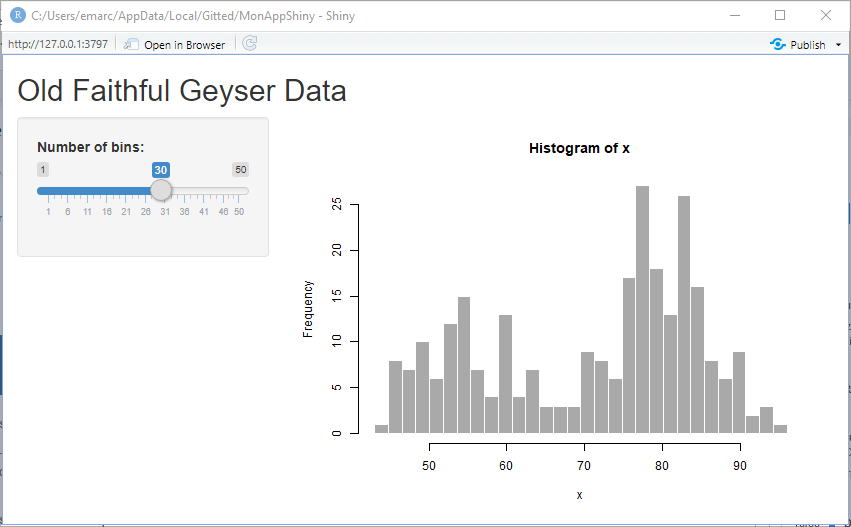
\includegraphics[width=0.8\linewidth]{images/shiny-geiser} 

}

\caption{Application Shiny \emph{Old Faithful Geyser Data}.}\label{fig:shiny-geiser}
\end{figure}

\normalsize

La correspondance entre la fenêtre affichée (figure \ref{fig:shiny-geiser}) et le code de la fonction \texttt{ui()} est simple à voir:

\begin{itemize}
\tightlist
\item
  le titre de l'application est affiché par la fonction \texttt{titlePanel()};
\item
  le curseur qui fixe le nombre de barres de l'histogramme est créé par \texttt{sliderInput()};
\item
  la fonction \texttt{sidebarLayout()} fixe la disposition des éléments de la page, \texttt{sidebarPanel} pour les contrôles de saisie et \texttt{mainPanel()} pour l'affichage du résultat.
\end{itemize}

Le résultat est affiché par la fonction \texttt{plotOutput()} dont l'argument est le nom d'un élément de \texttt{output}, la variable remplie par la fonction \texttt{server()}.

Toute modification d'un élément de l'interface, précisément d'un élément affiché par une fonction dont le nom se termine par \texttt{Input()} (il en existe pour tous les types d'entrées, par exemple \texttt{textInput()}) de \textbf{Shiny} provoque l'exécution de \texttt{server()} et la mise à jour des éléments de \texttt{output}.

\section{Application plus élaborée}\label{application-plus-uxe9laboruxe9e}

\subsection{Méthode de travail}\label{muxe9thode-de-travail}

Une application est créée en choisissant:

\begin{itemize}
\tightlist
\item
  une disposition de la fenêtre (\emph{layout});
\item
  les contrôles de saisie des paramètres (\emph{intput});
\item
  les contrôles d'affichage des résultats (\emph{output}).
\end{itemize}

Le code pour traiter les entrées et produire les sorties est ensuite écrit dans \texttt{server()}.

Le tutoriel de RStudio\footnote{\url{https://shiny.rstudio.com/tutorial/}} est très détaillé et doit être utilisé pour aller plus loin.

\subsection{Exemple}\label{exemple}

Cette application simple utilise le package \textbf{scholar} pour interroger Google Scholar et obtenir les données bibliométriques d'un auteur à partir de son identifiant.

Le fichier \texttt{app.R} contient tout le code et est construit progressivement ici.
L'application complète, avec des sorties graphiques en plus de sa version simplifiée présentée ici est disponible sur GitHub\footnote{\url{https://github.com/EricMarcon/bibliometrics}}.

Le début du code consiste à préparer l'exécution de l'application en chargeant les packages nécessaires:

\scriptsize

\begin{Shaded}
\begin{Highlighting}[]
\CommentTok{\# Prepare the application \#\#\#\#}

\CommentTok{\# Load packages}
\FunctionTok{library}\NormalTok{(}\StringTok{"shiny"}\NormalTok{)}
\FunctionTok{library}\NormalTok{(}\StringTok{"tidyverse"}\NormalTok{)}
\end{Highlighting}
\end{Shaded}

\normalsize

Le code de l'application complète intègre une fonction pour installer les packages manquants, à n'exécuter que quand l'application est exécutée sur un poste de travail (sur un serveur, la gestion des packages n'est pas du ressort de l'application).

L'interface utilisateur est la suivante:

\scriptsize

\begin{Shaded}
\begin{Highlighting}[]
\CommentTok{\# UI \#\#\#\#}
\NormalTok{ui }\OtherTok{\textless{}{-}} \FunctionTok{fluidPage}\NormalTok{(}
  \CommentTok{\# Application title}
  \FunctionTok{titlePanel}\NormalTok{(}\StringTok{"Bibliometrics"}\NormalTok{),}
  
  \FunctionTok{sidebarLayout}\NormalTok{(}
    \FunctionTok{sidebarPanel}\NormalTok{(}
      \FunctionTok{helpText}\NormalTok{(}\StringTok{"Enter the Google Scholar ID of an author."}\NormalTok{),}
      \FunctionTok{textInput}\NormalTok{(}\StringTok{"AuthorID"}\NormalTok{, }\StringTok{"Google Scholar ID"}\NormalTok{, }\StringTok{"4iLBmbUAAAAJ"}\NormalTok{),}
      \CommentTok{\# End of input}
      \FunctionTok{br}\NormalTok{(),}
      \CommentTok{\# Display author\textquotesingle{}s name and h}
      \FunctionTok{uiOutput}\NormalTok{(}\StringTok{"name"}\NormalTok{),}
      \FunctionTok{uiOutput}\NormalTok{(}\StringTok{"h"}\NormalTok{)}
\NormalTok{    ),}
    \CommentTok{\# Show plots in the main panel}
    \FunctionTok{mainPanel}\NormalTok{(}
      \FunctionTok{plotOutput}\NormalTok{(}\StringTok{"network"}\NormalTok{),}
      \FunctionTok{plotOutput}\NormalTok{(}\StringTok{"citations"}\NormalTok{)}
\NormalTok{    )}
\NormalTok{  )}
\NormalTok{)}
\end{Highlighting}
\end{Shaded}

\normalsize

La fenêtre de l'application est fluide, c'est-à-dire qu'elle se réorganise seule quand sa taille varie, et est composée d'un panneau latéral (pour la saisie et l'affichage de texte) et d'un panneau principal, pour l'affichage de graphiques.

Les éléments du panneau latéral sont:

\begin{itemize}
\tightlist
\item
  un texte d'aide: \texttt{helpText()};
\item
  un champ de texte à saisir, \texttt{textInput()}, dont les arguments sont le nom, le texte affiché, et la valeur par défaut (l'identifiant d'un auteur);
\item
  un saut de ligne: \texttt{br()};
\item
  des contrôles de sortie au format HTML: \texttt{uiOutput()}, dont l'argument unique est le nom.
\end{itemize}

Le panneau principal contient deux contrôles de sortie graphiques, \texttt{plotOutput()} dont l'argument est aussi le nom.

Le code à exécuter pour traiter les entrées et produire les sorties est dans la fonction \texttt{server()}.

\scriptsize

\begin{Shaded}
\begin{Highlighting}[]
\CommentTok{\# Server logic \#\#\#\#}
\NormalTok{server }\OtherTok{\textless{}{-}} \ControlFlowTok{function}\NormalTok{(input, output) \{}
  \CommentTok{\# Run the get\_profile function only once \#\#\#\#}
  \CommentTok{\# Store the author profile}
\NormalTok{  AuthorProfile }\OtherTok{\textless{}{-}} \FunctionTok{reactiveVal}\NormalTok{()}
  \CommentTok{\# Update it when input$AuthorID is changed}
  \FunctionTok{observeEvent}\NormalTok{(}
\NormalTok{    input}\SpecialCharTok{$}\NormalTok{AuthorID, }
    \FunctionTok{AuthorProfile}\NormalTok{(}\FunctionTok{get\_profile}\NormalTok{(input}\SpecialCharTok{$}\NormalTok{AuthorID))}
\NormalTok{  )}
  
  \CommentTok{\# Output \#\#\#\#}
\NormalTok{  output}\SpecialCharTok{$}\NormalTok{name }\OtherTok{\textless{}{-}} \FunctionTok{renderUI}\NormalTok{(\{}
    \FunctionTok{h2}\NormalTok{(}\FunctionTok{AuthorProfile}\NormalTok{()}\SpecialCharTok{$}\NormalTok{name)}
\NormalTok{  \})}
  
\NormalTok{  output}\SpecialCharTok{$}\NormalTok{h }\OtherTok{\textless{}{-}} \FunctionTok{renderUI}\NormalTok{(\{}
    \FunctionTok{a}\NormalTok{(}\AttributeTok{href =} \FunctionTok{paste0}\NormalTok{(}
      \StringTok{"https://scholar.google.com/citations?user="}\NormalTok{, }
\NormalTok{      input}\SpecialCharTok{$}\NormalTok{AuthorID),}
      \FunctionTok{paste}\NormalTok{(}\StringTok{"h index:"}\NormalTok{, }\FunctionTok{AuthorProfile}\NormalTok{()}\SpecialCharTok{$}\NormalTok{h\_index),}
      \AttributeTok{target =} \StringTok{"\_blank"}
\NormalTok{    )}
\NormalTok{  \})}
  
\NormalTok{  output}\SpecialCharTok{$}\NormalTok{citations }\OtherTok{\textless{}{-}} \FunctionTok{renderPlot}\NormalTok{(\{}
    \FunctionTok{get\_citation\_history}\NormalTok{(input}\SpecialCharTok{$}\NormalTok{AuthorID)  }\SpecialCharTok{\%\textgreater{}\%}
      \FunctionTok{ggplot}\NormalTok{(}\FunctionTok{aes}\NormalTok{(year, cites)) }\SpecialCharTok{+}
      \FunctionTok{geom\_segment}\NormalTok{(}\FunctionTok{aes}\NormalTok{(}\AttributeTok{xend =}\NormalTok{ year, }\AttributeTok{yend =} \DecValTok{0}\NormalTok{), }\AttributeTok{size =} \DecValTok{1}\NormalTok{, }\AttributeTok{color =} \StringTok{\textquotesingle{}darkgrey\textquotesingle{}}\NormalTok{) }\SpecialCharTok{+}
      \FunctionTok{geom\_point}\NormalTok{(}\AttributeTok{size =} \DecValTok{3}\NormalTok{, }\AttributeTok{color =} \StringTok{"firebrick"}\NormalTok{) }\SpecialCharTok{+}
      \FunctionTok{labs}\NormalTok{(}
        \AttributeTok{title =} \StringTok{"Citations per year"}\NormalTok{,}
        \AttributeTok{caption =} \StringTok{"Source: Google Scholar"}
\NormalTok{      )}
\NormalTok{  \})}
  
\NormalTok{  output}\SpecialCharTok{$}\NormalTok{network }\OtherTok{\textless{}{-}} \FunctionTok{renderPlot}\NormalTok{(\{}
    \FunctionTok{ggplot}\NormalTok{() }\SpecialCharTok{+} \FunctionTok{geom\_blank}\NormalTok{()}
\NormalTok{  \})}
\NormalTok{\}}
\end{Highlighting}
\end{Shaded}

\normalsize

Les informations nécessaires aux champs de sortie \texttt{\$name} et \texttt{\$h} (nom de l'auteur et indice h) sont obtenus par la fonction \texttt{get\_profile()} du package \textbf{scholar}.
Cette fonction interroge la page web Google Scholar de l'auteur et extrait les valeurs du résultat: c'est une traitement lourd, qu'il vaut mieux n'exécuter qu'une seule fois plutôt que deux, dans les fonctions \texttt{renderUI()} chargées de calculer les valeurs de \texttt{output\$h} et \texttt{output\$name}.

Le code le plus simple pour le faire serait le suivant:

\scriptsize

\begin{Shaded}
\begin{Highlighting}[]
  \CommentTok{\# Run the get\_profile function only once \#\#\#\#}
  \CommentTok{\# Store the author profile}
\NormalTok{  AuthorProfile }\OtherTok{\textless{}{-}} \FunctionTok{get\_profile}\NormalTok{(input}\SpecialCharTok{$}\NormalTok{AuthorID)}
\end{Highlighting}
\end{Shaded}

\normalsize

La difficulté de la programmation d'une application Shiny est que tout calcul se référant à un élément de l'interface d'entrée doit être \emph{réactif}.
Si ce dernier code était exécuté, le message d'erreur suivant apparaît:
\enquote{Operation not allowed without an active reactive context. (You tried to do something that can only be done from inside a reactive expression or observer.)}.

En pratique, l'exécution du code est lancée par la modification d'un contrôle d'entrée (ici: \texttt{intput\$AuthorID}).
Le code faisant référence à un de ces contrôles doit être en permanence en attente d'une modification: il doit donc placé dans des fonctions particulières comme \texttt{renderPlot()} dans l'application \emph{Old Faithful Geyser Data} ou \texttt{renderUI()} ici.
Le code suivant s'exécuterait sans erreur:

\scriptsize

\begin{Shaded}
\begin{Highlighting}[]
  \CommentTok{\# Output \#\#\#\#}
\NormalTok{  output}\SpecialCharTok{$}\NormalTok{name }\OtherTok{\textless{}{-}} \FunctionTok{renderUI}\NormalTok{(\{}
\NormalTok{    AuthorProfile }\OtherTok{\textless{}{-}} \FunctionTok{get\_profile}\NormalTok{(input}\SpecialCharTok{$}\NormalTok{AuthorID)}
    \FunctionTok{h2}\NormalTok{(AuthorProfile}\SpecialCharTok{$}\NormalTok{name)}
\NormalTok{  \})}
\end{Highlighting}
\end{Shaded}

\normalsize

L'appel à la valeur du contrôle \texttt{input\$AuthorID} a bien lieu dans une fonction réactive (mais \texttt{get\_profile()} devrait être utilisé une deuxième fois dans le calcul de \texttt{output\$h}, ce que nous voulons éviter).
La fonction \texttt{h2(AuthorProfile\$name)} produit du code HTML, un paragraphe de titre de niveau 2 dont la valeur est passée en argument.

Toutes les fonctions dont le nom commence par \texttt{render} dans le package \textbf{shiny} sont réactives, et chacune est destinée à produire un type de sortie différent, par exemple du texte (\texttt{renderText()}) ou du code HTML (\texttt{renderUI()}).

Si du code est nécessaire pour calculer des variables communes à plusieurs contrôles de sortie (\texttt{output\$name} et \texttt{output\$h}), il doit lui-même être réactif.
Deux fonctions sont très utiles:

\begin{itemize}
\tightlist
\item
  \texttt{observeEvent()} surveille les changements d'un contrôle d'entrée et exécute du code quand ils se produisent;
\item
  \texttt{reactiveVal()} permet de définir une variable réactive, qui sera modifiée par le code de \texttt{observeEvent()} et entraînera à son tour l'exécution d'autres fonctions réactives qui utilisent sa valeur.
\end{itemize}

Le code optimal crée donc une variable réactive pour y stocker le résultat de l'interrogation de Google Scholar:

\scriptsize

\begin{Shaded}
\begin{Highlighting}[]
  \CommentTok{\# Store the author profile}
\NormalTok{  AuthorProfile }\OtherTok{\textless{}{-}} \FunctionTok{reactiveVal}\NormalTok{()}
\end{Highlighting}
\end{Shaded}

\normalsize

La variable réactive est vide à ce stade.
Son utilisation est ensuite celle d'une fonction: \texttt{AuthorProfile(x)} lui attribue la valeur \texttt{x} et \texttt{AuthorProfile()}, sans argument, renvoie sa valeur.
La fonction \texttt{observeEvent()} est déclenchée quand \texttt{input\$AuthorID} est modifié et exécute le code passé en deuxième argument, ici la mise à jour de \texttt{AuthorProfile}.

\scriptsize

\begin{Shaded}
\begin{Highlighting}[]
  \CommentTok{\# Update it when input$AuthorID is changed}
  \FunctionTok{observeEvent}\NormalTok{(input}\SpecialCharTok{$}\NormalTok{AuthorID, }\FunctionTok{AuthorProfile}\NormalTok{(}\FunctionTok{get\_profile}\NormalTok{(input}\SpecialCharTok{$}\NormalTok{AuthorID)))}
\end{Highlighting}
\end{Shaded}

\normalsize

Enfin, les fonctions \texttt{renderUI()} qui fournissent les valeurs des contrôles de sortie utilisent la valeur de \texttt{AuthorProfile}:

\scriptsize

\begin{Shaded}
\begin{Highlighting}[]
  \CommentTok{\# Output \#\#\#\#}
\NormalTok{  output}\SpecialCharTok{$}\NormalTok{name }\OtherTok{\textless{}{-}} \FunctionTok{renderUI}\NormalTok{(\{}
     \FunctionTok{h2}\NormalTok{(}\FunctionTok{AuthorProfile}\NormalTok{()}\SpecialCharTok{$}\NormalTok{name)}
\NormalTok{  \})}
\end{Highlighting}
\end{Shaded}

\normalsize

Remarquer les parenthèses de \texttt{AuthorProfile()}, variable réactive, par opposition à la syntaxe \texttt{AuthorProfile\$name} pour une variable classique.

La valeur de \texttt{output\$h} est un lien internet, \texttt{\textless{}a\ href=...} en HTML, écrit par la fonction \texttt{a()} du package \textbf{htmltools} utilisé par \texttt{renderUI()}.

\scriptsize

\begin{Shaded}
\begin{Highlighting}[]
\NormalTok{  output}\SpecialCharTok{$}\NormalTok{h }\OtherTok{\textless{}{-}} \FunctionTok{renderUI}\NormalTok{(\{}
    \FunctionTok{a}\NormalTok{(}\AttributeTok{href =} \FunctionTok{paste0}\NormalTok{(}
        \StringTok{"https://scholar.google.com/citations?user="}\NormalTok{, input}\SpecialCharTok{$}\NormalTok{AuthorID}
\NormalTok{      ),}
      \FunctionTok{paste}\NormalTok{(}\StringTok{"h index:"}\NormalTok{, }\FunctionTok{AuthorProfile}\NormalTok{()}\SpecialCharTok{$}\NormalTok{h\_index),}
      \AttributeTok{target =} \StringTok{"\_blank"}
\NormalTok{    )}
\NormalTok{  \})}
\end{Highlighting}
\end{Shaded}

\normalsize

Le lien est vers la page Google Scholar de l'auteur.
La valeur affichée est son indice h.
L'argument \texttt{target\ =\ "\_blank"} indique que le lien doit être ouvert dans une nouvelle fenêtre du navigateur.

Le graphique \texttt{output\$citations} est créé par la fonction réactive \texttt{renderPlot()}.
Les données fournies par la fonction \texttt{get\_citation\_history()} de \textbf{scholar} (qui interroge l'API de Google Scholar) sont traitées par \texttt{ggplot()}.

Enfin, le graphique \texttt{output\$network} est un graphique vide dans cette version simplifiée de l'application.

L'application complète reprend ce code en y ajoutant le traitement des erreurs dans le cas où le code de l'auteur n'existe par sur Google Scholar et le graphique du réseau des co-auteurs.

\section{Hébergement}\label{sec:hebergement-shiny}

Une application Shiny n'est pas forcément hébergée par un serveur web: elle peut être exécutée sur les postes de travail des utilisateurs s'ils disposent de R.

Pour un usage plus large, un serveur dédié est nécessaire.
Shinyapps.io\footnote{\url{https://www.shinyapps.io/}} est un service de RStudio qui permet d'héberger gratuitement 5 applications Shiny avec un temps de fonctionnement maximal de 5 heures par mois.

Il faut tout d'abord ouvrir un compte sur le site, de préférence avec ses identifiants GitHub.
Pour permettre la gestion des applications en ligne directement depuis RStudio, il faut installer ensuite le package \textbf{rsconnect} et le paramétrer:

\scriptsize

\begin{Shaded}
\begin{Highlighting}[]
\NormalTok{rsconnect}\SpecialCharTok{::}\FunctionTok{setAccountInfo}\NormalTok{(}
  \AttributeTok{name =} \StringTok{\textquotesingle{}prenom.nom\textquotesingle{}}\NormalTok{,}
    \AttributeTok{token =} \StringTok{\textquotesingle{}xxx\textquotesingle{}}\NormalTok{,}
    \AttributeTok{secret =} \StringTok{\textquotesingle{}\textless{}SECRET\textgreater{}\textquotesingle{}}
\NormalTok{)}
\end{Highlighting}
\end{Shaded}

\normalsize

Le code exact, avec le nom d'utilisateur et le jeton à utiliser, sont affichés sur la page d'accueil de Shinyapps.io: cliquer sur \enquote{Show Secret}, copier le code et le coller dans la console de RStudio pour l'exécuter.
Un bouton \enquote{Publish} est disponible juste à droite du bouton \enquote{Run App}.
Cliquer dessus et valider la publication (figure \ref{fig:shiny-publish}).



\scriptsize

\begin{figure}

{\centering 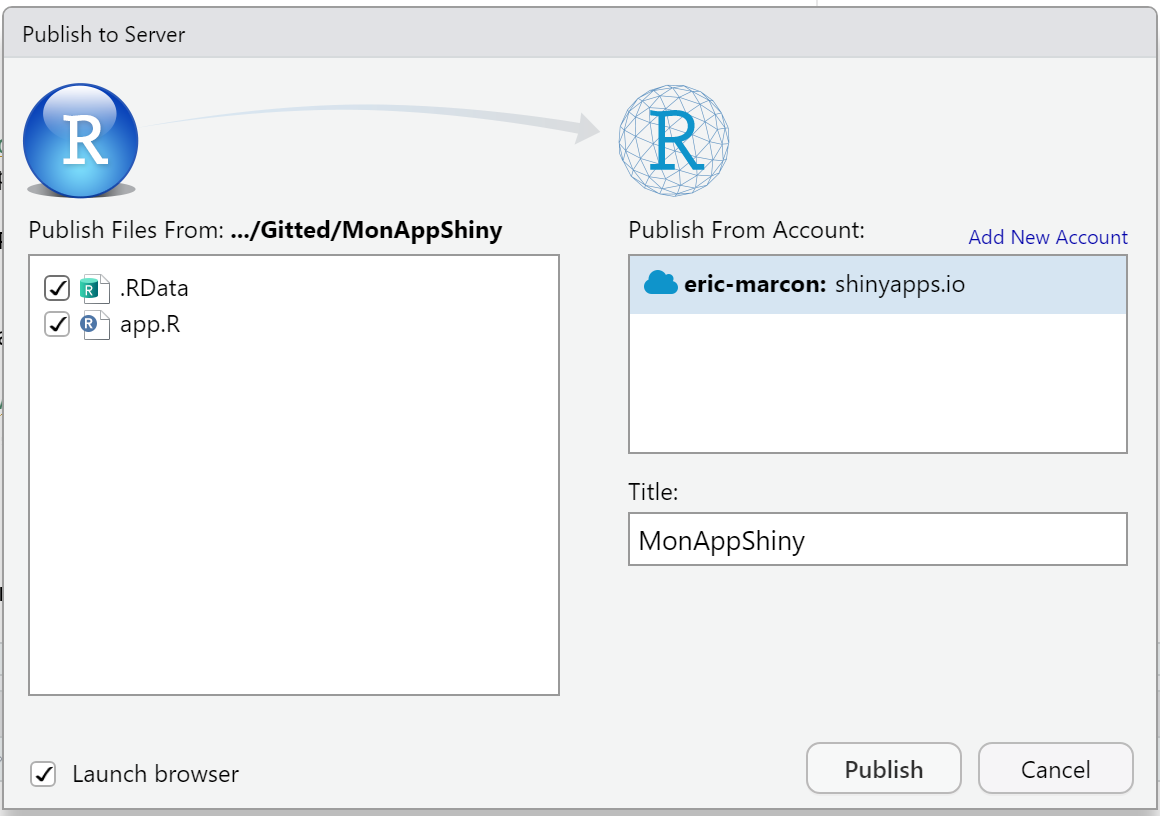
\includegraphics[width=0.8\linewidth]{images/shiny-publish} 

}

\caption{Publication de l'application Shiny sur Shinyapps.io.}\label{fig:shiny-publish}
\end{figure}

\normalsize

L'application est maintenant accessible à l'adresse \url{https://prenom-nom.shinyapps.io/MonAppShiny/}

L'application \enquote{Bibliometrics} ne fonctionne pas sur Shinyapps.io parce que la façon dont le package \textbf{Scholar} interroge Google Scholar n'est pas supportée.
La plupart des applications Shiny fonctionnent sans difficulté, tant qu'elles ne nécessitent pas de fonctionnalités réseau complexes.

\chapter{Enseigner avec R}\label{chap-enseigner}

\toc{1}

R, RStudio et GitHub fournissent des outils pour enseigner.

Le package \textbf{learnr} permet de réaliser des tutoriels interactifs.

On verra aussi comment utiliser les salles de classe GitHub (\emph{GitHub Classrooms}) qui permettent de diffuser à une classe (une liste d'étudiants disposant d'un compte GitHub) un modèle de dépôt (un début de projet R) que chaque étudiant devra développer et publier.
Les outils de la salle de classe permettent d'évaluer le travail fourni assez simplement.

\section{learnr}\label{learnr}

\textbf{learnr} permet de rendre interactifs les bouts de code de n'importe quel document produit par R Markdown en HTML, en les transformant en applications Shiny.
La documentation sur le site de RStudio\footnote{\url{https://rstudio.github.io/learnr/}} est très claire et ne sera pas reprise ici: nous verrons seulement comment commencer et comment diffuser les tutoriels.

\subsection{Premier tutoriel}\label{premier-tutoriel}

Utiliser comme pour tous les documents le menu \enquote{File \textgreater{} New File \textgreater{} RMarkdown\ldots{}} et créer un nouveau document à partir d'un modèle \enquote{Interactive Tutorial}.
L'assistant crée un dossier du nom choisi, à transformer en projet R et passer sous contrôle de source, comme pour tous les documents vus précédemment (voir section \ref{sec:memo}).

Pour exécuter le tutoriel, cliquer sur le bouton \enquote{Run Document} qui se trouve à place habituelle du bouton \enquote{Tricoter}.

Les tutoriels peuvent inclure des exercices, qui sont des bouts de code avec l'option \texttt{exercise=TRUE}.
Ces exercices sont affichés sous la forme d'une fenêtre de code modifiable et exécutable par l'utilisateur.
Des indices peuvent être donnés\footnote{\url{https://rstudio.github.io/learnr/exercises.html\#Hints_and_Solutions}}, un bouton ajouté pour afficher la solution, une limite de temps peut être fixée\footnote{\url{https://rstudio.github.io/learnr/exercises.html\#Time_Limits}}, et le code comme son résultat peuvent être comparés à une valeur attendue\footnote{\url{https://rstudio.github.io/learnr/exercises.html\#Exercise_Checking}}.

Des quizz\footnote{\url{https://rstudio.github.io/learnr/questions.html}} peuvent être ajoutés, sous la forme de questionnaires à choix multiples ou uniques.

La progression de l'utilisateur dans le tutoriel (code saisi, réponses aux questions\ldots) est sauvegardée par \textbf{learnr} sur le poste de travail.
Un tutoriel peut être arrêté puis repris sans perte de données.
En revanche, il n'y a pas de moyen simple de récupérer ces données pour une évaluation par le formateur par exemple.

\subsection{Diffusion}\label{diffusion}

Les tutoriels peuvent être diffusés en copiant les fichiers ou en indiquant aux utilisateurs de cloner les projets GitHub qui les contiennent.

Ils peuvent aussi être hébergés sur Shinyapps.io (voir section \ref{sec:hebergement-shiny}).

Enfin, ils peuvent être inclus dans un package\footnote{\url{https://rstudio.github.io/learnr/publishing.html\#R_Package}}.

\section{GitHub Classrooms}\label{github-classrooms}

GitHub Classrooms permet de diffuser à un public étudiant des dépôts GitHub à modifier et de contrôler le résultat.
Les applications sont aussi bien l'apprentissage de R que la production de documents, pour un travail personnel ou un examen par exemple.

\subsection{Inscription}\label{inscription}

Pour commencer à utiliser l'outil, il faut ouvrir un compte.
Sur le site de GitHub Classrooms\footnote{\url{https://classroom.github.com/}}, cliquer sur \enquote{Sign in} et utiliser son compte GitHub pour s'authentifier.

\subsection{Organisations}\label{organisations}

L'étape suivant consiste à créer une organisation GitHub.
Une organisation GitHub contient essentiellement des membres (titulaires d'un compte GitHub) et des dépôts accessibles à l'adresse \url{https://github.com/Organisation/Depot}.

La façon la plus simple de travailler consiste à créer une organisation par cours mais d'autres approches sont possibles dans des structures utilisant intensivement l'outil.
L'organisation crée pour l'exemple est ici \enquote{Cours-R}\footnote{\url{https://github.com/Cours-R}}.

Une adresse de messagerie est nécessaire (utiliser la même que celle de son compte GitHub) et l'organisation doit être déclarée comme appartenant à son compte personnel.

Si l'organisation n'est pas visible sur la page de GitHub Classrooms, cliquer sur \enquote{Grant us access}.

\subsection{Nouvelle salle de classe}\label{nouvelle-salle-de-classe}

Une salle de classe (\emph{classroom}) est peuplée d'étudiants qui recevront des tâches (\emph{assignments}) à exécuter.

Cliquer sur \emph{New Classroom}.
Sélectionner l'organisation en charge de l'administration de la salle de classe.

Saisir le nom de la salle de classe: une bonne pratique est de la préfixer par le nom du cours et d'ajouter le nom de la session, par exemple \enquote{Cours-R-2020-EdGuyane}.

Ne pas ajouter de collaborateurs (ce sera possible plus tard), et saisir éventuellement la liste des étudiants (un nom par ligne, possible plus tard aussi).
La classe est créée.

Toutes les salles de classe sont visibles depuis la page d'accueil de GitHub Classrooms\footnote{\url{https://classroom.github.com/classrooms}}.
Cliquer sur un nom pour en ouvrir une.
Le bouton \enquote{Settings} permet de changer son nom ou de la supprimer.
Le bouton \enquote{TAs and Admins} permet d'ajouter des collaborateurs, c'est-à-dire d'autres utilisateurs GitHub qui pourront administrer la salle de classe.

Le bouton \enquote{Students} permet d'ajouter des étudiants.
La liste de nom est libre, sans format obligatoire.
Cliquer sur \enquote{Create Roster} pour l'activer.
Les noms doivent ensuite être liés à des comptes GitHub: ce travail peut être fait par l'administrateur ou par les étudiants eux-mêmes quand ils recevront la première tâche à effectuer.
Chaque étudiant doit avoir un compte sur GitHub.

\subsection{Préparer un modèle de dépôt}\label{pruxe9parer-un-moduxe8le-de-duxe9puxf4t}

Une tâche est un dépôt GitHub à modifier.
Par exemple\footnote{\url{https://github.com/EricMarcon/Cours-R-Memo/settings}}, créer un dépôt contenant un projet R avec un fichier Markdown décrivant le travail à faire et éventuellement une partie du code nécessaire pour y parvenir, les autres fichiers du modèle R Markdown utilisé et un fichier de données.

Ouvrir les propriétés du dépôt sur GitHub et cocher la case \emph{Template Repository} pour en faire un modèle.

\subsubsection{Assigner une tâche}\label{assigner-une-tuxe2che}

Ouvrir une salle de classe et cliquer sur \enquote{New Assignment}.

Saisir un titre explicite pour les étudiants, une date limite optionnelle et choisir \enquote{Individual Assignment}.

Par défaut, le nom de la tâche sert de préfixe pour le nom des dépôts des étudiants mais il peut être remplacé par un préfixe choisi.
Quand les étudiants rendront leur travail, tous les dépôts de toutes les tâches seront stockés dans l'organisation.

Le dépôt crée sur le compte de chaque étudiant peut être privé ou public, selon que l'on souhaite que les étudiants puissent voir le travail des autres ou non.
Donner le droit d'administration et rendre le site public si les étudiants doivent pouvoir activer les pages GitHub pour présenter le résultat de leur travail.
Cliquer sur \enquote{Continue}.

Sélectionner le dépôt modèle (\emph{starter code}) puis cliquer sur \enquote{Continue} puis \enquote{Create Assignment}.

La nouvelle tâche est créée.
Elle est associée à un lien d'invitation qu'il faut copier et envoyer aux étudiants.
Quand ils cliqueront sur le lien, ils atteindront une page GitHub qui leur permettra d'associer leur compte à un nom de la liste (aucun contrôle n'est possible: le premier connecté peut s'associer à n'importe quel nom).
Ils pourront ensuite créer un nouveau projet RStudio à partir du dépôt GitHub créé automatiquement par GitHub Classrooms, modifier ce projet selon les consignes de travail et le pousser sur GitHub.
Le dépôt se trouve sur le compte de l'organisation à laquelle la classe est reliée, et est suffixé par l'identifiant GitHub de l'étudiant.

\subsubsection{Contrôler le travail des étudiants}\label{contruxf4ler-le-travail-des-uxe9tudiants}

Il est possible d'afficher chaque dépôt crée par les étudiants à partir de la page de la tâche sur GitHub Classrooms.
Si le travail à produire est un document rédigé, demander aux étudiants de le placer dans les pages GitHub du dépôt pour le lire directement en ligne.

L'assistant GitHub Classrooms\footnote{\url{https://classroom.github.com/assistant}} permet de télécharger en une fois tous les dépôts des étudiants pour les corriger sur son poste de travail.

\chapter{Conclusion}\label{chap-conclusion}

L'environnement de travail de R et RStudio permet de produire tous types de documents avec un langage unique.

L'objectif de reproductibilité des résultats est atteint en intégrant les traitements statistiques et la rédaction.
Le travail collaboratif est permis par l'utilisation systématique du contrôle de source et de GitHub.
La présentation des résultats est assurée par les pages GitHub et des modèles de documents couvrant la majorité des besoins.

Pour les pauses, R fournit même quelques jeux dans le package \textbf{fun}, dont le célèbre démineur:

\scriptsize

\begin{Shaded}
\begin{Highlighting}[]
\CommentTok{\# Installation du package}
\FunctionTok{install.packages}\NormalTok{(}\StringTok{"fun"}\NormalTok{)}
\CommentTok{\# Ouverture d\textquotesingle{}une fenêtre X et exécution}
\ControlFlowTok{if}\NormalTok{ (}\FunctionTok{interactive}\NormalTok{()) \{}
  \ControlFlowTok{if}\NormalTok{ (.Platform}\SpecialCharTok{$}\NormalTok{OS.type }\SpecialCharTok{==} \StringTok{"windows"}\NormalTok{) \{}
    \FunctionTok{x11}\NormalTok{() }
\NormalTok{  \} }\ControlFlowTok{else}\NormalTok{ \{ }
    \FunctionTok{x11}\NormalTok{(}\AttributeTok{type =} \StringTok{"Xlib"}\NormalTok{)}
\NormalTok{  \}}
\NormalTok{  fun}\SpecialCharTok{::}\FunctionTok{mine\_sweeper}\NormalTok{()}
\NormalTok{\}}
\end{Highlighting}
\end{Shaded}

\normalsize

Ce document n'a pas pour objectif d'être exhaustif sur les possibilités de R mais plutôt de présenter une méthode de travail et des moyens simples de l'appliquer rapidement.
On se reportera aux ouvrages plus détaillés cités dans le texte pour approfondir tel ou tel point.

Il est mis à jour régulièrement en fonction de l'évolution des outils disponibles.


% Bibliography
%%%%%%%%%%%%%%%%%%%%%%%%%%%%%%%%%%%%%%%%%%%%%%%%%%%%%%%%%%

\backmatter
\SmallMargins

\printbibliography
\onecolumn


% Tables (of tables, of figures)
%%%%%%%%%%%%%%%%%%%%%%%%%%%%%%%%%%%%%%%%%%%%%%%%%%%%%%%%%%


\cleardoublepage
\LargeMargins
\listoffigures


% After-body (LaTeX code inclusion)
%%%%%%%%%%%%%%%%%%%%%%%%%%%%%%%%%%%%%%%%%%%%%%%%%%%%%%%%%%




% Back cover
%%%%%%%%%%%%%%%%%%%%%%%%%%%%%%%%%%%%%%%%%%%%%%%%%%%%%%%%%%%

% Even page, small margins, no running head, no page number.
\evenpage
\SmallMargins
\thispagestyle{empty}

\begin{normalsize}

\begin{description}

\selectlanguage{french}
\item[Résumé]
Cet ouvrage propose une organisation du travail autour de R et RStudio pour, au-delà des statistiques, rédiger des documents efficacement avec R Markdown, aux formats variés (mémos, articles scientifiques, mémoires d'étudiants, livres, diaporamas), créer son site web et des applications R en ligne (Shiny), produire des packages et utiliser R pour l'enseignement.
\item[]
.
~\\

\end{description}

\end{normalsize}


\end{document}
